\documentclass[a4paper,titlepage,11pt,twosides,floatssmall]{mwrep}
\usepackage[left=2.5cm,right=2.5cm,top=2.5cm,bottom=2.5cm]{geometry}
\usepackage[OT1]{fontenc}
\usepackage{polski}
\usepackage{amsmath}
\usepackage{amsfonts}
\usepackage{amssymb}
\usepackage{graphicx}
\usepackage{url}
\usepackage{tikz}
\usetikzlibrary{arrows,calc,decorations.markings,math,arrows.meta}
\usepackage{rotating}
\usepackage[percent]{overpic}
\usepackage[cp1250]{inputenc}
\usepackage{xcolor}
\usepackage{pgfplots}
\usetikzlibrary{pgfplots.groupplots}
\usepackage{listings}
\usepackage{matlab-prettifier}
\usepackage{enumitem,amssymb}
\definecolor{szary}{rgb}{0.95,0.95,0.95}
\usepackage{siunitx}
\sisetup{detect-weight,exponent-product=\cdot,output-decimal-marker={,},per-mode=symbol,binary-units=true,range-phrase={-},range-units=single}
\SendSettingsToPgf
%konfiguracje pakietu listings
\lstset{
	backgroundcolor=\color{szary},
	frame=single,
	breaklines=true,
}
\lstdefinestyle{customlatex}{
	basicstyle=\footnotesize\ttfamily,
	%basicstyle=\small\ttfamily,
}
\lstdefinestyle{customc}{
	breaklines=true,
	frame=tb,
	language=C,
	xleftmargin=0pt,
	showstringspaces=false,
	basicstyle=\small\ttfamily,
	keywordstyle=\bfseries\color{green!40!black},
	commentstyle=\itshape\color{purple!40!black},
	identifierstyle=\color{blue},
	stringstyle=\color{orange},
}
\lstdefinestyle{custommatlab}{
	captionpos=t,
	breaklines=true,
	frame=tb,
	xleftmargin=0pt,
	language=matlab,
	showstringspaces=false,
	%basicstyle=\footnotesize\ttfamily,
	basicstyle=\scriptsize\ttfamily,
	keywordstyle=\bfseries\color{green!40!black},
	commentstyle=\itshape\color{purple!40!black},
	identifierstyle=\color{blue},
	stringstyle=\color{orange},
}

%wymiar tekstu (bez żywej paginy)
\textwidth 160mm \textheight 247mm

%ustawienia pakietu pgfplots
\pgfplotsset{
tick label style={font=\scriptsize},
label style={font=\small},
legend style={font=\small},
title style={font=\small}
}

\def\figurename{Rys.}
\def\tablename{Tab.}

%konfiguracja liczby pływających elementów
\setcounter{topnumber}{0}%2
\setcounter{bottomnumber}{3}%1
\setcounter{totalnumber}{5}%3
\renewcommand{\textfraction}{0.01}%0.2
\renewcommand{\topfraction}{0.95}%0.7
\renewcommand{\bottomfraction}{0.95}%0.3
\renewcommand{\floatpagefraction}{0.35}%0.5

\begin{document}
\frenchspacing
\pagestyle{uheadings}

%strona tytułowa
\title{\bf Sprawozdanie z projektu i ćwiczenia laboratoryjnego nr 1, zadanie nr 3\vskip 0.1cm}
\author{Wojciech Rokicki, Radosław Tuzimek, Jakub Gruszecki}
\date{2020}

\makeatletter
\renewcommand{\maketitle}{\begin{titlepage}
\begin{center}{\LARGE {\bf
Wydział Elektroniki i Technik Informacyjnych}}\\
\vspace{0.4cm}
{\LARGE {\bf Politechnika Warszawska}}\\
\vspace{0.3cm}
\end{center}
\vspace{5cm}
\begin{center}
{\bf \LARGE Projektowanie układów sterowania\\ (projekt grupowy) \vskip 0.1cm}
\end{center}
\vspace{1cm}
\begin{center}
{\bf \LARGE \@title}
\end{center}
\vspace{2cm}
\begin{center}
{\bf \Large \@author \par}
\end{center}
\vspace*{\stretch{6}}
\begin{center}
\bf{\large{Warszawa, \@date\vskip 0.1cm}}
\end{center}
\end{titlepage}
}
\makeatother

\maketitle

\tableofcontents
\chapter{Sprawdzenie poprawno�ci punktu pracy}

\section{Poprawno�� warto�ci sygna��w w punkcie pracy}
W celu sprawdzenia poprawno�ci warto�ci sygna��w $U_{\mathrm{pp}}$ oraz $Y_{\mathrm{pp}}$ obiekt zosta� pobudzony sygna�em o warto�ci: $U_{\mathrm{pp}}=\num{0}$. Warto�ci sygna��w w punkcie pracy b�d� poprawne, je�li sygna� wyj�ciowy przyjmie warto�� sta�� $Y_{\mathrm{pp}}=\num{0}$.

\begin{figure}[h!]
\centering
% This file was created by matlab2tikz.
%
\definecolor{mycolor1}{rgb}{0.00000,0.44700,0.74100}%
%
\begin{tikzpicture}

\begin{axis}[%
width=4.521in,
height=1.493in,
at={(0.758in,2.554in)},
scale only axis,
xmin=0,
xmax=400,
ymin=-1,
ymax=1,
axis background/.style={fill=white},
title style={font=\bfseries},
title={U},
legend style={legend cell align=left, align=left, draw=white!15!black}
]
\addplot [color=mycolor1]
  table[row sep=crcr]{%
1	0\\
2	0\\
3	0\\
4	0\\
5	0\\
6	0\\
7	0\\
8	0\\
9	0\\
10	0\\
11	0\\
12	0\\
13	0\\
14	0\\
15	0\\
16	0\\
17	0\\
18	0\\
19	0\\
20	0\\
21	0\\
22	0\\
23	0\\
24	0\\
25	0\\
26	0\\
27	0\\
28	0\\
29	0\\
30	0\\
31	0\\
32	0\\
33	0\\
34	0\\
35	0\\
36	0\\
37	0\\
38	0\\
39	0\\
40	0\\
41	0\\
42	0\\
43	0\\
44	0\\
45	0\\
46	0\\
47	0\\
48	0\\
49	0\\
50	0\\
51	0\\
52	0\\
53	0\\
54	0\\
55	0\\
56	0\\
57	0\\
58	0\\
59	0\\
60	0\\
61	0\\
62	0\\
63	0\\
64	0\\
65	0\\
66	0\\
67	0\\
68	0\\
69	0\\
70	0\\
71	0\\
72	0\\
73	0\\
74	0\\
75	0\\
76	0\\
77	0\\
78	0\\
79	0\\
80	0\\
81	0\\
82	0\\
83	0\\
84	0\\
85	0\\
86	0\\
87	0\\
88	0\\
89	0\\
90	0\\
91	0\\
92	0\\
93	0\\
94	0\\
95	0\\
96	0\\
97	0\\
98	0\\
99	0\\
100	0\\
101	0\\
102	0\\
103	0\\
104	0\\
105	0\\
106	0\\
107	0\\
108	0\\
109	0\\
110	0\\
111	0\\
112	0\\
113	0\\
114	0\\
115	0\\
116	0\\
117	0\\
118	0\\
119	0\\
120	0\\
121	0\\
122	0\\
123	0\\
124	0\\
125	0\\
126	0\\
127	0\\
128	0\\
129	0\\
130	0\\
131	0\\
132	0\\
133	0\\
134	0\\
135	0\\
136	0\\
137	0\\
138	0\\
139	0\\
140	0\\
141	0\\
142	0\\
143	0\\
144	0\\
145	0\\
146	0\\
147	0\\
148	0\\
149	0\\
150	0\\
151	0\\
152	0\\
153	0\\
154	0\\
155	0\\
156	0\\
157	0\\
158	0\\
159	0\\
160	0\\
161	0\\
162	0\\
163	0\\
164	0\\
165	0\\
166	0\\
167	0\\
168	0\\
169	0\\
170	0\\
171	0\\
172	0\\
173	0\\
174	0\\
175	0\\
176	0\\
177	0\\
178	0\\
179	0\\
180	0\\
181	0\\
182	0\\
183	0\\
184	0\\
185	0\\
186	0\\
187	0\\
188	0\\
189	0\\
190	0\\
191	0\\
192	0\\
193	0\\
194	0\\
195	0\\
196	0\\
197	0\\
198	0\\
199	0\\
200	0\\
201	0\\
202	0\\
203	0\\
204	0\\
205	0\\
206	0\\
207	0\\
208	0\\
209	0\\
210	0\\
211	0\\
212	0\\
213	0\\
214	0\\
215	0\\
216	0\\
217	0\\
218	0\\
219	0\\
220	0\\
221	0\\
222	0\\
223	0\\
224	0\\
225	0\\
226	0\\
227	0\\
228	0\\
229	0\\
230	0\\
231	0\\
232	0\\
233	0\\
234	0\\
235	0\\
236	0\\
237	0\\
238	0\\
239	0\\
240	0\\
241	0\\
242	0\\
243	0\\
244	0\\
245	0\\
246	0\\
247	0\\
248	0\\
249	0\\
250	0\\
251	0\\
252	0\\
253	0\\
254	0\\
255	0\\
256	0\\
257	0\\
258	0\\
259	0\\
260	0\\
261	0\\
262	0\\
263	0\\
264	0\\
265	0\\
266	0\\
267	0\\
268	0\\
269	0\\
270	0\\
271	0\\
272	0\\
273	0\\
274	0\\
275	0\\
276	0\\
277	0\\
278	0\\
279	0\\
280	0\\
281	0\\
282	0\\
283	0\\
284	0\\
285	0\\
286	0\\
287	0\\
288	0\\
289	0\\
290	0\\
291	0\\
292	0\\
293	0\\
294	0\\
295	0\\
296	0\\
297	0\\
298	0\\
299	0\\
300	0\\
301	0\\
302	0\\
303	0\\
304	0\\
305	0\\
306	0\\
307	0\\
308	0\\
309	0\\
310	0\\
311	0\\
312	0\\
313	0\\
314	0\\
315	0\\
316	0\\
317	0\\
318	0\\
319	0\\
320	0\\
321	0\\
322	0\\
323	0\\
324	0\\
325	0\\
326	0\\
327	0\\
328	0\\
329	0\\
330	0\\
331	0\\
332	0\\
333	0\\
334	0\\
335	0\\
336	0\\
337	0\\
338	0\\
339	0\\
340	0\\
341	0\\
342	0\\
343	0\\
344	0\\
345	0\\
346	0\\
347	0\\
348	0\\
349	0\\
350	0\\
351	0\\
352	0\\
353	0\\
354	0\\
355	0\\
356	0\\
357	0\\
358	0\\
359	0\\
360	0\\
361	0\\
362	0\\
363	0\\
364	0\\
365	0\\
366	0\\
367	0\\
368	0\\
369	0\\
370	0\\
371	0\\
372	0\\
373	0\\
374	0\\
375	0\\
376	0\\
377	0\\
378	0\\
379	0\\
380	0\\
381	0\\
382	0\\
383	0\\
384	0\\
385	0\\
386	0\\
387	0\\
388	0\\
389	0\\
390	0\\
391	0\\
392	0\\
393	0\\
394	0\\
395	0\\
396	0\\
397	0\\
398	0\\
399	0\\
400	0\\
};

\end{axis}

\begin{axis}[%
width=4.521in,
height=1.493in,
at={(0.758in,0.481in)},
scale only axis,
xmin=0,
xmax=400,
ymin=-1,
ymax=1,
axis background/.style={fill=white},
title style={font=\bfseries},
title={Y},
legend style={legend cell align=left, align=left, draw=white!15!black}
]
\addplot [color=mycolor1]
  table[row sep=crcr]{%
1	0\\
2	0\\
3	0\\
4	0\\
5	0\\
6	0\\
7	0\\
8	0\\
9	0\\
10	0\\
11	0\\
12	0\\
13	0\\
14	0\\
15	0\\
16	0\\
17	0\\
18	0\\
19	0\\
20	0\\
21	0\\
22	0\\
23	0\\
24	0\\
25	0\\
26	0\\
27	0\\
28	0\\
29	0\\
30	0\\
31	0\\
32	0\\
33	0\\
34	0\\
35	0\\
36	0\\
37	0\\
38	0\\
39	0\\
40	0\\
41	0\\
42	0\\
43	0\\
44	0\\
45	0\\
46	0\\
47	0\\
48	0\\
49	0\\
50	0\\
51	0\\
52	0\\
53	0\\
54	0\\
55	0\\
56	0\\
57	0\\
58	0\\
59	0\\
60	0\\
61	0\\
62	0\\
63	0\\
64	0\\
65	0\\
66	0\\
67	0\\
68	0\\
69	0\\
70	0\\
71	0\\
72	0\\
73	0\\
74	0\\
75	0\\
76	0\\
77	0\\
78	0\\
79	0\\
80	0\\
81	0\\
82	0\\
83	0\\
84	0\\
85	0\\
86	0\\
87	0\\
88	0\\
89	0\\
90	0\\
91	0\\
92	0\\
93	0\\
94	0\\
95	0\\
96	0\\
97	0\\
98	0\\
99	0\\
100	0\\
101	0\\
102	0\\
103	0\\
104	0\\
105	0\\
106	0\\
107	0\\
108	0\\
109	0\\
110	0\\
111	0\\
112	0\\
113	0\\
114	0\\
115	0\\
116	0\\
117	0\\
118	0\\
119	0\\
120	0\\
121	0\\
122	0\\
123	0\\
124	0\\
125	0\\
126	0\\
127	0\\
128	0\\
129	0\\
130	0\\
131	0\\
132	0\\
133	0\\
134	0\\
135	0\\
136	0\\
137	0\\
138	0\\
139	0\\
140	0\\
141	0\\
142	0\\
143	0\\
144	0\\
145	0\\
146	0\\
147	0\\
148	0\\
149	0\\
150	0\\
151	0\\
152	0\\
153	0\\
154	0\\
155	0\\
156	0\\
157	0\\
158	0\\
159	0\\
160	0\\
161	0\\
162	0\\
163	0\\
164	0\\
165	0\\
166	0\\
167	0\\
168	0\\
169	0\\
170	0\\
171	0\\
172	0\\
173	0\\
174	0\\
175	0\\
176	0\\
177	0\\
178	0\\
179	0\\
180	0\\
181	0\\
182	0\\
183	0\\
184	0\\
185	0\\
186	0\\
187	0\\
188	0\\
189	0\\
190	0\\
191	0\\
192	0\\
193	0\\
194	0\\
195	0\\
196	0\\
197	0\\
198	0\\
199	0\\
200	0\\
201	0\\
202	0\\
203	0\\
204	0\\
205	0\\
206	0\\
207	0\\
208	0\\
209	0\\
210	0\\
211	0\\
212	0\\
213	0\\
214	0\\
215	0\\
216	0\\
217	0\\
218	0\\
219	0\\
220	0\\
221	0\\
222	0\\
223	0\\
224	0\\
225	0\\
226	0\\
227	0\\
228	0\\
229	0\\
230	0\\
231	0\\
232	0\\
233	0\\
234	0\\
235	0\\
236	0\\
237	0\\
238	0\\
239	0\\
240	0\\
241	0\\
242	0\\
243	0\\
244	0\\
245	0\\
246	0\\
247	0\\
248	0\\
249	0\\
250	0\\
251	0\\
252	0\\
253	0\\
254	0\\
255	0\\
256	0\\
257	0\\
258	0\\
259	0\\
260	0\\
261	0\\
262	0\\
263	0\\
264	0\\
265	0\\
266	0\\
267	0\\
268	0\\
269	0\\
270	0\\
271	0\\
272	0\\
273	0\\
274	0\\
275	0\\
276	0\\
277	0\\
278	0\\
279	0\\
280	0\\
281	0\\
282	0\\
283	0\\
284	0\\
285	0\\
286	0\\
287	0\\
288	0\\
289	0\\
290	0\\
291	0\\
292	0\\
293	0\\
294	0\\
295	0\\
296	0\\
297	0\\
298	0\\
299	0\\
300	0\\
301	0\\
302	0\\
303	0\\
304	0\\
305	0\\
306	0\\
307	0\\
308	0\\
309	0\\
310	0\\
311	0\\
312	0\\
313	0\\
314	0\\
315	0\\
316	0\\
317	0\\
318	0\\
319	0\\
320	0\\
321	0\\
322	0\\
323	0\\
324	0\\
325	0\\
326	0\\
327	0\\
328	0\\
329	0\\
330	0\\
331	0\\
332	0\\
333	0\\
334	0\\
335	0\\
336	0\\
337	0\\
338	0\\
339	0\\
340	0\\
341	0\\
342	0\\
343	0\\
344	0\\
345	0\\
346	0\\
347	0\\
348	0\\
349	0\\
350	0\\
351	0\\
352	0\\
353	0\\
354	0\\
355	0\\
356	0\\
357	0\\
358	0\\
359	0\\
360	0\\
361	0\\
362	0\\
363	0\\
364	0\\
365	0\\
366	0\\
367	0\\
368	0\\
369	0\\
370	0\\
371	0\\
372	0\\
373	0\\
374	0\\
375	0\\
376	0\\
377	0\\
378	0\\
379	0\\
380	0\\
381	0\\
382	0\\
383	0\\
384	0\\
385	0\\
386	0\\
387	0\\
388	0\\
389	0\\
390	0\\
391	0\\
392	0\\
393	0\\
394	0\\
395	0\\
396	0\\
397	0\\
398	0\\
399	0\\
400	0\\
};

\end{axis}

\begin{axis}[%
width=5.833in,
height=4.375in,
at={(0in,0in)},
scale only axis,
xmin=0,
xmax=1,
ymin=0,
ymax=1,
axis line style={draw=none},
ticks=none,
axis x line*=bottom,
axis y line*=left,
legend style={legend cell align=left, align=left, draw=white!15!black}
]
\end{axis}
\end{tikzpicture}%
\caption{Przebiegi sygna��w u(k), y(k) w punkcie pracy}
\label{punkt_pracy}
\end{figure}

\section{Wnioski}
Na podstawie rysunku \ref{punkt_pracy} wida�, �e dla sta�ej warto�ci sygna�u steruj�cego $U_{\mathrm{pp}}=\num{0}$ wyj�cie obiektu przyjmuje sta�� warto��, r�wn� $Y_{\mathrm{pp}}=~\num{0}$. Jest to dow�d na to, �e podane warto�ci sygna��w wej�ciowego sterowania oraz wyj�ciowego w punkcie pracy s� poprawne.

\section{Implementacja}
Do przeprowadzenia eksperymentu wykorzystany zosta� skrypt \verb+zad1.m+.
\chapter{Odpowiedzi skokowe i charakterystyka statyczna}

\section{Wyznaczenie dpowiedzi skokowych}
W celu wyznaczenia odpowiedzi skokowych obiekt pobudzony zosta� czterema skokami sygna�u steruj�cego w chwili k=21. Sygna� steruj�cy zmienia� si� o $dU$=0,1 od $U_{min}$=0,9 do $U_{max}$=1,3.

\begin{figure}[h!]
\centering
% This file was created by matlab2tikz.
%
%The latest updates can be retrieved from
%  http://www.mathworks.com/matlabcentral/fileexchange/22022-matlab2tikz-matlab2tikz
%where you can also make suggestions and rate matlab2tikz.
%
\definecolor{mycolor1}{rgb}{0.00000,0.44700,0.74100}%
\definecolor{mycolor2}{rgb}{0.85000,0.32500,0.09800}%
\definecolor{mycolor3}{rgb}{0.92900,0.69400,0.12500}%
\definecolor{mycolor4}{rgb}{0.49400,0.18400,0.55600}%
%
\begin{tikzpicture}

\begin{axis}[%
width=4.521in,
height=1.488in,
at={(0.758in,2.554in)},
scale only axis,
xmin=0,
xmax=600,
ymin=1.36443365695792,
ymax=2.63556634304209,
axis background/.style={fill=white},
title style={font=\bfseries},
title={Sygnal wyjsciowy},
legend style={legend cell align=left, align=left, draw=white!15!black}
]
\addplot [color=mycolor1]
  table[row sep=crcr]{%
1	2\\
2	2\\
3	2\\
4	2\\
5	2\\
6	2\\
7	2\\
8	2\\
9	2\\
10	2\\
11	2\\
12	2\\
13	2\\
14	2\\
15	2\\
16	2\\
17	2\\
18	2\\
19	2\\
20	2\\
21	2\\
22	2\\
23	2\\
24	2\\
25	2\\
26	2\\
27	2\\
28	2\\
29	2\\
30	2\\
31	1.9979816\\
32	1.99235773848\\
33	1.98371668135674\\
34	1.97257503023226\\
35	1.95938553170158\\
36	1.94454408239941\\
37	1.92839600996488\\
38	1.91124170226892\\
39	1.89334165017042\\
40	1.87492096267203\\
41	1.85617340756908\\
42	1.83726502546675\\
43	1.81833736032739\\
44	1.79951034545341\\
45	1.78088487996797\\
46	1.76254512738566\\
47	1.74456056473254\\
48	1.72698780784788\\
49	1.70987223594765\\
50	1.69324943622739\\
51	1.6771464872043\\
52	1.66158309762431\\
53	1.64657261606932\\
54	1.63212292487534\\
55	1.61823723059774\\
56	1.60491476202054\\
57	1.59215138559002\\
58	1.57994014714617\\
59	1.56827174791886\\
60	1.55713496193878\\
61	1.54651700127759\\
62	1.53640383486921\\
63	1.52678046606834\\
64	1.51763117356549\\
65	1.50893971979504\\
66	1.50068953053909\\
67	1.49286384903899\\
68	1.48544586757572\\
69	1.47841883916507\\
70	1.47176617172999\\
71	1.46547150685825\\
72	1.45951878502523\\
73	1.45389229895657\\
74	1.44857673662161\\
75	1.44355721518399\\
76	1.43881930708764\\
77	1.43434905932444\\
78	1.43013300681122\\
79	1.42615818069774\\
80	1.42241211233249\\
81	1.41888283352845\\
82	1.41555887369521\\
83	1.41242925433613\\
84	1.40948348134926\\
85	1.40671153551659\\
86	1.40410386151866\\
87	1.40165135576871\\
88	1.39934535332284\\
89	1.39717761408892\\
90	1.39514030852713\\
91	1.39322600300849\\
92	1.39142764497447\\
93	1.3897385480199\\
94	1.38815237700302\\
95	1.38666313327078\\
96	1.3852651400727\\
97	1.38395302822474\\
98	1.38272172207325\\
99	1.38156642579973\\
100	1.38048261009867\\
101	1.37946599925363\\
102	1.37851255863013\\
103	1.37761848259882\\
104	1.37678018289737\\
105	1.37599427743579\\
106	1.37525757954611\\
107	1.37456708767486\\
108	1.37391997551386\\
109	1.37331358256314\\
110	1.37274540511797\\
111	1.37221308767055\\
112	1.37171441471586\\
113	1.37124730295023\\
114	1.37080979385063\\
115	1.370400046622\\
116	1.37001633149978\\
117	1.36965702339446\\
118	1.36932059586489\\
119	1.36900561540721\\
120	1.36871073604618\\
121	1.36843469421589\\
122	1.36817630391714\\
123	1.36793445213884\\
124	1.36770809453132\\
125	1.36749625131951\\
126	1.36729800344442\\
127	1.36711248892183\\
128	1.36693889940721\\
129	1.36677647695653\\
130	1.3666245109729\\
131	1.36648233532925\\
132	1.36634932565809\\
133	1.36622489679907\\
134	1.36610850039628\\
135	1.36599962263679\\
136	1.36589778212304\\
137	1.36580252787144\\
138	1.36571343743031\\
139	1.36563011511037\\
140	1.36555219032161\\
141	1.36547931601024\\
142	1.3654111671902\\
143	1.36534743956378\\
144	1.36528784822606\\
145	1.36523212644847\\
146	1.36518002453673\\
147	1.36513130875884\\
148	1.36508576033904\\
149	1.36504317451375\\
150	1.36500335964587\\
151	1.36496613639389\\
152	1.36493133693264\\
153	1.36489880422244\\
154	1.36486839132382\\
155	1.36483996075501\\
156	1.36481338388965\\
157	1.36478854039223\\
158	1.36476531768891\\
159	1.36474361047169\\
160	1.36472332023373\\
161	1.36470435483407\\
162	1.36468662808968\\
163	1.3646700593935\\
164	1.36465457335651\\
165	1.36464009947257\\
166	1.36462657180455\\
167	1.36461392869038\\
168	1.36460211246778\\
169	1.36459106921663\\
170	1.36458074851764\\
171	1.36457110322652\\
172	1.36456208926255\\
173	1.36455366541068\\
174	1.36454579313632\\
175	1.36453843641193\\
176	1.36453156155485\\
177	1.36452513707541\\
178	1.36451913353494\\
179	1.36451352341275\\
180	1.36450828098183\\
181	1.36450338219243\\
182	1.36449880456324\\
183	1.36449452707947\\
184	1.36449053009767\\
185	1.3644867952565\\
186	1.36448330539347\\
187	1.36448004446688\\
188	1.36447699748293\\
189	1.36447415042752\\
190	1.36447149020241\\
191	1.3644690045656\\
192	1.36446668207555\\
193	1.36446451203894\\
194	1.36446248446195\\
195	1.3644605900046\\
196	1.36445881993812\\
197	1.36445716610503\\
198	1.36445562088186\\
199	1.3644541771443\\
200	1.36445282823459\\
201	1.364451567931\\
202	1.3644503904194\\
203	1.3644492902666\\
204	1.3644482623954\\
205	1.36444730206139\\
206	1.36444640483111\\
207	1.36444556656177\\
208	1.36444478338219\\
209	1.36444405167504\\
210	1.36444336806021\\
211	1.36444272937932\\
212	1.36444213268116\\
213	1.36444157520813\\
214	1.36444105438357\\
215	1.36444056779991\\
216	1.36444011320757\\
217	1.36443968850462\\
218	1.36443929172711\\
219	1.36443892104001\\
220	1.36443857472877\\
221	1.3644382511914\\
222	1.36443794893113\\
223	1.36443766654946\\
224	1.36443740273975\\
225	1.36443715628117\\
226	1.3644369260331\\
227	1.36443671092982\\
228	1.36443650997566\\
229	1.36443632224033\\
230	1.36443614685468\\
231	1.36443598300667\\
232	1.36443582993763\\
233	1.36443568693873\\
234	1.36443555334775\\
235	1.36443542854596\\
236	1.36443531195533\\
237	1.36443520303581\\
238	1.36443510128285\\
239	1.36443500622508\\
240	1.3644349174221\\
241	1.36443483446249\\
242	1.36443475696186\\
243	1.36443468456111\\
244	1.36443461692473\\
245	1.36443455373929\\
246	1.36443449471197\\
247	1.36443443956921\\
248	1.36443438805542\\
249	1.36443433993185\\
250	1.36443429497543\\
251	1.36443425297777\\
252	1.36443421374419\\
253	1.36443417709281\\
254	1.36443414285372\\
255	1.36443411086817\\
256	1.36443408098788\\
257	1.36443405307431\\
258	1.36443402699803\\
259	1.36443400263813\\
260	1.36443397988166\\
261	1.3644339586231\\
262	1.36443393876386\\
263	1.36443392021185\\
264	1.36443390288103\\
265	1.36443388669104\\
266	1.36443387156678\\
267	1.36443385743812\\
268	1.36443384423952\\
269	1.36443383190977\\
270	1.36443382039168\\
271	1.36443380963183\\
272	1.3644337995803\\
273	1.36443379019048\\
274	1.36443378141881\\
275	1.3644337732246\\
276	1.36443376556983\\
277	1.364433758419\\
278	1.36443375173894\\
279	1.36443374549865\\
280	1.36443373966919\\
281	1.36443373422352\\
282	1.36443372913636\\
283	1.36443372438412\\
284	1.36443371994475\\
285	1.36443371579765\\
286	1.36443371192359\\
287	1.36443370830459\\
288	1.36443370492385\\
289	1.36443370176569\\
290	1.36443369881546\\
291	1.36443369605947\\
292	1.36443369348494\\
293	1.3644336910799\\
294	1.36443368883322\\
295	1.36443368673446\\
296	1.36443368477388\\
297	1.36443368294238\\
298	1.36443368123148\\
299	1.36443367963322\\
300	1.36443367814019\\
301	1.36443367674546\\
302	1.36443367544257\\
303	1.36443367422546\\
304	1.36443367308849\\
305	1.36443367202638\\
306	1.3644336710342\\
307	1.36443367010735\\
308	1.36443366924153\\
309	1.36443366843271\\
310	1.36443366767715\\
311	1.36443366697134\\
312	1.364433666312\\
313	1.36443366569608\\
314	1.36443366512071\\
315	1.36443366458322\\
316	1.36443366408113\\
317	1.36443366361209\\
318	1.36443366317394\\
319	1.36443366276464\\
320	1.36443366238229\\
321	1.36443366202511\\
322	1.36443366169146\\
323	1.36443366137977\\
324	1.3644336610886\\
325	1.36443366081661\\
326	1.36443366056253\\
327	1.36443366032518\\
328	1.36443366010345\\
329	1.36443365989633\\
330	1.36443365970284\\
331	1.3644336595221\\
332	1.36443365935325\\
333	1.36443365919553\\
334	1.36443365904818\\
335	1.36443365891055\\
336	1.36443365878197\\
337	1.36443365866186\\
338	1.36443365854966\\
339	1.36443365844485\\
340	1.36443365834694\\
341	1.36443365825547\\
342	1.36443365817003\\
343	1.36443365809022\\
344	1.36443365801566\\
345	1.36443365794601\\
346	1.36443365788094\\
347	1.36443365782016\\
348	1.36443365776339\\
349	1.36443365771035\\
350	1.3644336576608\\
351	1.36443365761452\\
352	1.36443365757128\\
353	1.36443365753089\\
354	1.36443365749316\\
355	1.36443365745792\\
356	1.36443365742499\\
357	1.36443365739424\\
358	1.36443365736551\\
359	1.36443365733867\\
360	1.3644336573136\\
361	1.36443365729018\\
362	1.3644336572683\\
363	1.36443365724786\\
364	1.36443365722877\\
365	1.36443365721093\\
366	1.36443365719427\\
367	1.36443365717871\\
368	1.36443365716417\\
369	1.36443365715059\\
370	1.3644336571379\\
371	1.36443365712605\\
372	1.36443365711498\\
373	1.36443365710464\\
374	1.36443365709498\\
375	1.36443365708595\\
376	1.36443365707752\\
377	1.36443365706964\\
378	1.36443365706229\\
379	1.36443365705541\\
380	1.36443365704899\\
381	1.364433657043\\
382	1.36443365703739\\
383	1.36443365703216\\
384	1.36443365702727\\
385	1.36443365702271\\
386	1.36443365701844\\
387	1.36443365701445\\
388	1.36443365701073\\
389	1.36443365700725\\
390	1.36443365700401\\
391	1.36443365700097\\
392	1.36443365699814\\
393	1.36443365699549\\
394	1.36443365699302\\
395	1.3644336569907\\
396	1.36443365698855\\
397	1.36443365698653\\
398	1.36443365698465\\
399	1.36443365698289\\
400	1.36443365698124\\
401	1.36443365697971\\
402	1.36443365697827\\
403	1.36443365697693\\
404	1.36443365697568\\
405	1.36443365697451\\
406	1.36443365697342\\
407	1.3644336569724\\
408	1.36443365697145\\
409	1.36443365697056\\
410	1.36443365696972\\
411	1.36443365696895\\
412	1.36443365696822\\
413	1.36443365696754\\
414	1.36443365696691\\
415	1.36443365696632\\
416	1.36443365696576\\
417	1.36443365696525\\
418	1.36443365696477\\
419	1.36443365696432\\
420	1.3644336569639\\
421	1.3644336569635\\
422	1.36443365696314\\
423	1.36443365696279\\
424	1.36443365696247\\
425	1.36443365696217\\
426	1.36443365696189\\
427	1.36443365696163\\
428	1.36443365696139\\
429	1.36443365696116\\
430	1.36443365696094\\
431	1.36443365696075\\
432	1.36443365696056\\
433	1.36443365696039\\
434	1.36443365696022\\
435	1.36443365696007\\
436	1.36443365695993\\
437	1.3644336569598\\
438	1.36443365695968\\
439	1.36443365695956\\
440	1.36443365695945\\
441	1.36443365695935\\
442	1.36443365695926\\
443	1.36443365695917\\
444	1.36443365695909\\
445	1.36443365695901\\
446	1.36443365695894\\
447	1.36443365695887\\
448	1.36443365695881\\
449	1.36443365695875\\
450	1.3644336569587\\
451	1.36443365695865\\
452	1.3644336569586\\
453	1.36443365695855\\
454	1.36443365695851\\
455	1.36443365695847\\
456	1.36443365695843\\
457	1.3644336569584\\
458	1.36443365695837\\
459	1.36443365695834\\
460	1.36443365695831\\
461	1.36443365695829\\
462	1.36443365695826\\
463	1.36443365695824\\
464	1.36443365695822\\
465	1.3644336569582\\
466	1.36443365695818\\
467	1.36443365695816\\
468	1.36443365695815\\
469	1.36443365695813\\
470	1.36443365695812\\
471	1.36443365695811\\
472	1.36443365695809\\
473	1.36443365695808\\
474	1.36443365695807\\
475	1.36443365695806\\
476	1.36443365695805\\
477	1.36443365695805\\
478	1.36443365695804\\
479	1.36443365695803\\
480	1.36443365695802\\
481	1.36443365695802\\
482	1.36443365695801\\
483	1.364433656958\\
484	1.364433656958\\
485	1.36443365695799\\
486	1.36443365695799\\
487	1.36443365695798\\
488	1.36443365695798\\
489	1.36443365695798\\
490	1.36443365695797\\
491	1.36443365695797\\
492	1.36443365695797\\
493	1.36443365695797\\
494	1.36443365695796\\
495	1.36443365695796\\
496	1.36443365695796\\
497	1.36443365695796\\
498	1.36443365695795\\
499	1.36443365695795\\
500	1.36443365695795\\
501	1.36443365695795\\
502	1.36443365695794\\
503	1.36443365695794\\
504	1.36443365695794\\
505	1.36443365695794\\
506	1.36443365695794\\
507	1.36443365695794\\
508	1.36443365695794\\
509	1.36443365695793\\
510	1.36443365695793\\
511	1.36443365695793\\
512	1.36443365695793\\
513	1.36443365695793\\
514	1.36443365695793\\
515	1.36443365695793\\
516	1.36443365695793\\
517	1.36443365695793\\
518	1.36443365695793\\
519	1.36443365695792\\
520	1.36443365695792\\
521	1.36443365695792\\
522	1.36443365695792\\
523	1.36443365695792\\
524	1.36443365695792\\
525	1.36443365695792\\
526	1.36443365695792\\
527	1.36443365695792\\
528	1.36443365695792\\
529	1.36443365695792\\
530	1.36443365695792\\
531	1.36443365695792\\
532	1.36443365695792\\
533	1.36443365695792\\
534	1.36443365695792\\
535	1.36443365695792\\
536	1.36443365695792\\
537	1.36443365695792\\
538	1.36443365695792\\
539	1.36443365695792\\
540	1.36443365695792\\
541	1.36443365695792\\
542	1.36443365695792\\
543	1.36443365695792\\
544	1.36443365695792\\
545	1.36443365695792\\
546	1.36443365695792\\
547	1.36443365695792\\
548	1.36443365695792\\
549	1.36443365695792\\
550	1.36443365695792\\
551	1.36443365695792\\
552	1.36443365695792\\
553	1.36443365695792\\
554	1.36443365695792\\
555	1.36443365695792\\
556	1.36443365695792\\
557	1.36443365695792\\
558	1.36443365695792\\
559	1.36443365695792\\
560	1.36443365695792\\
561	1.36443365695792\\
562	1.36443365695792\\
563	1.36443365695792\\
564	1.36443365695792\\
565	1.36443365695792\\
566	1.36443365695792\\
567	1.36443365695792\\
568	1.36443365695792\\
569	1.36443365695792\\
570	1.36443365695792\\
571	1.36443365695792\\
572	1.36443365695792\\
573	1.36443365695792\\
574	1.36443365695792\\
575	1.36443365695792\\
576	1.36443365695792\\
577	1.36443365695792\\
578	1.36443365695792\\
579	1.36443365695792\\
580	1.36443365695792\\
581	1.36443365695792\\
582	1.36443365695792\\
583	1.36443365695792\\
584	1.36443365695792\\
585	1.36443365695792\\
586	1.36443365695792\\
587	1.36443365695792\\
588	1.36443365695792\\
589	1.36443365695792\\
590	1.36443365695792\\
591	1.36443365695792\\
592	1.36443365695792\\
593	1.36443365695792\\
594	1.36443365695792\\
595	1.36443365695792\\
596	1.36443365695792\\
597	1.36443365695792\\
598	1.36443365695792\\
599	1.36443365695792\\
600	1.36443365695792\\
};
\addlegendentry{U = 0.9}

\addplot [color=mycolor2]
  table[row sep=crcr]{%
1	2\\
2	2\\
3	2\\
4	2\\
5	2\\
6	2\\
7	2\\
8	2\\
9	2\\
10	2\\
11	2\\
12	2\\
13	2\\
14	2\\
15	2\\
16	2\\
17	2\\
18	2\\
19	2\\
20	2\\
21	2\\
22	2\\
23	2\\
24	2\\
25	2\\
26	2\\
27	2\\
28	2\\
29	2\\
30	2\\
31	1.9989908\\
32	1.99617886924\\
33	1.99185834067837\\
34	1.98628751511613\\
35	1.97969276585079\\
36	1.97227204119971\\
37	1.96419800498244\\
38	1.95562085113446\\
39	1.94667082508521\\
40	1.93746048133602\\
41	1.92808670378454\\
42	1.91863251273338\\
43	1.9091686801637\\
44	1.8997551727267\\
45	1.89044243998399\\
46	1.88127256369283\\
47	1.87228028236627\\
48	1.86349390392394\\
49	1.85493611797383\\
50	1.8466247181137\\
51	1.83857324360215\\
52	1.83079154881216\\
53	1.82328630803466\\
54	1.81606146243767\\
55	1.80911861529887\\
56	1.80245738101027\\
57	1.79607569279501\\
58	1.78997007357309\\
59	1.78413587395943\\
60	1.77856748096939\\
61	1.7732585006388\\
62	1.7682019174346\\
63	1.76339023303417\\
64	1.75881558678275\\
65	1.75446985989752\\
66	1.75034476526955\\
67	1.7464319245195\\
68	1.74272293378786\\
69	1.73920941958254\\
70	1.735883085865\\
71	1.73273575342913\\
72	1.72975939251262\\
73	1.72694614947828\\
74	1.72428836831081\\
75	1.721778607592\\
76	1.71940965354382\\
77	1.71717452966222\\
78	1.71506650340561\\
79	1.71307909034887\\
80	1.71120605616624\\
81	1.70944141676423\\
82	1.7077794368476\\
83	1.70621462716806\\
84	1.70474174067463\\
85	1.70335576775829\\
86	1.70205193075933\\
87	1.70082567788435\\
88	1.69967267666142\\
89	1.69858880704446\\
90	1.69757015426356\\
91	1.69661300150424\\
92	1.69571382248723\\
93	1.69486927400994\\
94	1.69407618850151\\
95	1.69333156663539\\
96	1.69263257003635\\
97	1.69197651411237\\
98	1.69136086103662\\
99	1.69078321289986\\
100	1.69024130504933\\
101	1.68973299962681\\
102	1.68925627931506\\
103	1.68880924129941\\
104	1.68839009144868\\
105	1.68799713871789\\
106	1.68762878977305\\
107	1.68728354383743\\
108	1.68695998775693\\
109	1.68665679128157\\
110	1.68637270255898\\
111	1.68610654383527\\
112	1.68585720735793\\
113	1.68562365147511\\
114	1.68540489692531\\
115	1.68520002331099\\
116	1.68500816574989\\
117	1.68482851169723\\
118	1.68466029793244\\
119	1.6845028077036\\
120	1.68435536802309\\
121	1.68421734710794\\
122	1.68408815195857\\
123	1.68396722606942\\
124	1.68385404726566\\
125	1.68374812565975\\
126	1.68364900172221\\
127	1.68355624446091\\
128	1.6834694497036\\
129	1.68338823847826\\
130	1.68331225548645\\
131	1.68324116766463\\
132	1.68317466282904\\
133	1.68311244839954\\
134	1.68305425019814\\
135	1.68299981131839\\
136	1.68294889106152\\
137	1.68290126393572\\
138	1.68285671871515\\
139	1.68281505755518\\
140	1.6827760951608\\
141	1.68273965800512\\
142	1.6827055835951\\
143	1.68267371978189\\
144	1.68264392411303\\
145	1.68261606322423\\
146	1.68259001226836\\
147	1.68256565437942\\
148	1.68254288016952\\
149	1.68252158725688\\
150	1.68250167982293\\
151	1.68248306819694\\
152	1.68246566846632\\
153	1.68244940211122\\
154	1.68243419566191\\
155	1.6824199803775\\
156	1.68240669194483\\
157	1.68239427019611\\
158	1.68238265884445\\
159	1.68237180523584\\
160	1.68236166011687\\
161	1.68235217741703\\
162	1.68234331404484\\
163	1.68233502969675\\
164	1.68232728667825\\
165	1.68232004973628\\
166	1.68231328590228\\
167	1.68230696434519\\
168	1.68230105623389\\
169	1.68229553460832\\
170	1.68229037425882\\
171	1.68228555161326\\
172	1.68228104463127\\
173	1.68227683270534\\
174	1.68227289656816\\
175	1.68226921820597\\
176	1.68226578077742\\
177	1.68226256853771\\
178	1.68225956676747\\
179	1.68225676170637\\
180	1.68225414049091\\
181	1.68225169109622\\
182	1.68224940228162\\
183	1.68224726353974\\
184	1.68224526504883\\
185	1.68224339762825\\
186	1.68224165269674\\
187	1.68224002223344\\
188	1.68223849874147\\
189	1.68223707521376\\
190	1.6822357451012\\
191	1.6822345022828\\
192	1.68223334103777\\
193	1.68223225601947\\
194	1.68223124223097\\
195	1.6822302950023\\
196	1.68222940996906\\
197	1.68222858305251\\
198	1.68222781044093\\
199	1.68222708857215\\
200	1.68222641411729\\
201	1.6822257839655\\
202	1.6822251952097\\
203	1.6822246451333\\
204	1.6822241311977\\
205	1.68222365103069\\
206	1.68222320241556\\
207	1.68222278328089\\
208	1.6822223916911\\
209	1.68222202583752\\
210	1.68222168403011\\
211	1.68222136468966\\
212	1.68222106634058\\
213	1.68222078760407\\
214	1.68222052719179\\
215	1.68222028389996\\
216	1.68222005660379\\
217	1.68221984425231\\
218	1.68221964586356\\
219	1.68221946052\\
220	1.68221928736438\\
221	1.6822191255957\\
222	1.68221897446556\\
223	1.68221883327473\\
224	1.68221870136987\\
225	1.68221857814058\\
226	1.68221846301655\\
227	1.68221835546491\\
228	1.68221825498783\\
229	1.68221816112016\\
230	1.68221807342734\\
231	1.68221799150334\\
232	1.68221791496881\\
233	1.68221784346937\\
234	1.68221777667387\\
235	1.68221771427298\\
236	1.68221765597766\\
237	1.6822176015179\\
238	1.68221755064142\\
239	1.68221750311253\\
240	1.68221745871105\\
241	1.68221741723124\\
242	1.68221737848093\\
243	1.68221734228055\\
244	1.68221730846236\\
245	1.68221727686964\\
246	1.68221724735598\\
247	1.6822172197846\\
248	1.68221719402771\\
249	1.68221716996592\\
250	1.68221714748771\\
251	1.68221712648888\\
252	1.68221710687209\\
253	1.6822170885464\\
254	1.68221707142685\\
255	1.68221705543408\\
256	1.68221704049394\\
257	1.68221702653715\\
258	1.68221701349901\\
259	1.68221700131907\\
260	1.68221698994083\\
261	1.68221697931155\\
262	1.68221696938193\\
263	1.68221696010592\\
264	1.68221695144051\\
265	1.68221694334552\\
266	1.68221693578339\\
267	1.68221692871906\\
268	1.68221692211976\\
269	1.68221691595488\\
270	1.68221691019584\\
271	1.68221690481591\\
272	1.68221689979015\\
273	1.68221689509524\\
274	1.6822168907094\\
275	1.6822168866123\\
276	1.68221688278491\\
277	1.6822168792095\\
278	1.68221687586947\\
279	1.68221687274933\\
280	1.6822168698346\\
281	1.68221686711176\\
282	1.68221686456818\\
283	1.68221686219206\\
284	1.68221685997238\\
285	1.68221685789883\\
286	1.6822168559618\\
287	1.68221685415229\\
288	1.68221685246192\\
289	1.68221685088285\\
290	1.68221684940773\\
291	1.68221684802974\\
292	1.68221684674247\\
293	1.68221684553995\\
294	1.68221684441661\\
295	1.68221684336723\\
296	1.68221684238694\\
297	1.68221684147119\\
298	1.68221684061574\\
299	1.68221683981661\\
300	1.68221683907009\\
301	1.68221683837273\\
302	1.68221683772128\\
303	1.68221683711273\\
304	1.68221683654424\\
305	1.68221683601319\\
306	1.6822168355171\\
307	1.68221683505368\\
308	1.68221683462076\\
309	1.68221683421636\\
310	1.68221683383858\\
311	1.68221683348567\\
312	1.682216833156\\
313	1.68221683284804\\
314	1.68221683256035\\
315	1.68221683229161\\
316	1.68221683204056\\
317	1.68221683180605\\
318	1.68221683158697\\
319	1.68221683138232\\
320	1.68221683119115\\
321	1.68221683101256\\
322	1.68221683084573\\
323	1.68221683068989\\
324	1.68221683054431\\
325	1.68221683040831\\
326	1.68221683028127\\
327	1.68221683016259\\
328	1.68221683005173\\
329	1.68221682994817\\
330	1.68221682985143\\
331	1.68221682976105\\
332	1.68221682967663\\
333	1.68221682959777\\
334	1.6822168295241\\
335	1.68221682945528\\
336	1.68221682939099\\
337	1.68221682933094\\
338	1.68221682927484\\
339	1.68221682922243\\
340	1.68221682917347\\
341	1.68221682912774\\
342	1.68221682908502\\
343	1.68221682904511\\
344	1.68221682900783\\
345	1.68221682897301\\
346	1.68221682894048\\
347	1.68221682891009\\
348	1.6822168288817\\
349	1.68221682885518\\
350	1.68221682883041\\
351	1.68221682880726\\
352	1.68221682878565\\
353	1.68221682876545\\
354	1.68221682874659\\
355	1.68221682872896\\
356	1.6822168287125\\
357	1.68221682869712\\
358	1.68221682868276\\
359	1.68221682866934\\
360	1.6822168286568\\
361	1.68221682864509\\
362	1.68221682863415\\
363	1.68221682862393\\
364	1.68221682861439\\
365	1.68221682860547\\
366	1.68221682859714\\
367	1.68221682858936\\
368	1.68221682858209\\
369	1.6822168285753\\
370	1.68221682856895\\
371	1.68221682856303\\
372	1.68221682855749\\
373	1.68221682855232\\
374	1.68221682854749\\
375	1.68221682854298\\
376	1.68221682853876\\
377	1.68221682853482\\
378	1.68221682853114\\
379	1.68221682852771\\
380	1.6822168285245\\
381	1.6822168285215\\
382	1.6822168285187\\
383	1.68221682851608\\
384	1.68221682851364\\
385	1.68221682851135\\
386	1.68221682850922\\
387	1.68221682850723\\
388	1.68221682850537\\
389	1.68221682850363\\
390	1.682216828502\\
391	1.68221682850049\\
392	1.68221682849907\\
393	1.68221682849774\\
394	1.68221682849651\\
395	1.68221682849535\\
396	1.68221682849427\\
397	1.68221682849326\\
398	1.68221682849232\\
399	1.68221682849144\\
400	1.68221682849062\\
401	1.68221682848985\\
402	1.68221682848913\\
403	1.68221682848846\\
404	1.68221682848784\\
405	1.68221682848725\\
406	1.68221682848671\\
407	1.6822168284862\\
408	1.68221682848572\\
409	1.68221682848528\\
410	1.68221682848486\\
411	1.68221682848447\\
412	1.68221682848411\\
413	1.68221682848377\\
414	1.68221682848345\\
415	1.68221682848316\\
416	1.68221682848288\\
417	1.68221682848262\\
418	1.68221682848238\\
419	1.68221682848216\\
420	1.68221682848195\\
421	1.68221682848175\\
422	1.68221682848157\\
423	1.68221682848139\\
424	1.68221682848123\\
425	1.68221682848108\\
426	1.68221682848094\\
427	1.68221682848081\\
428	1.68221682848069\\
429	1.68221682848058\\
430	1.68221682848047\\
431	1.68221682848037\\
432	1.68221682848028\\
433	1.68221682848019\\
434	1.68221682848011\\
435	1.68221682848003\\
436	1.68221682847996\\
437	1.6822168284799\\
438	1.68221682847984\\
439	1.68221682847978\\
440	1.68221682847972\\
441	1.68221682847967\\
442	1.68221682847963\\
443	1.68221682847958\\
444	1.68221682847954\\
445	1.6822168284795\\
446	1.68221682847947\\
447	1.68221682847943\\
448	1.6822168284794\\
449	1.68221682847937\\
450	1.68221682847935\\
451	1.68221682847932\\
452	1.6822168284793\\
453	1.68221682847927\\
454	1.68221682847925\\
455	1.68221682847923\\
456	1.68221682847922\\
457	1.6822168284792\\
458	1.68221682847918\\
459	1.68221682847917\\
460	1.68221682847915\\
461	1.68221682847914\\
462	1.68221682847913\\
463	1.68221682847912\\
464	1.68221682847911\\
465	1.6822168284791\\
466	1.68221682847909\\
467	1.68221682847908\\
468	1.68221682847907\\
469	1.68221682847907\\
470	1.68221682847906\\
471	1.68221682847905\\
472	1.68221682847905\\
473	1.68221682847904\\
474	1.68221682847904\\
475	1.68221682847903\\
476	1.68221682847903\\
477	1.68221682847902\\
478	1.68221682847902\\
479	1.68221682847901\\
480	1.68221682847901\\
481	1.68221682847901\\
482	1.682216828479\\
483	1.682216828479\\
484	1.682216828479\\
485	1.682216828479\\
486	1.68221682847899\\
487	1.68221682847899\\
488	1.68221682847899\\
489	1.68221682847899\\
490	1.68221682847899\\
491	1.68221682847898\\
492	1.68221682847898\\
493	1.68221682847898\\
494	1.68221682847898\\
495	1.68221682847898\\
496	1.68221682847898\\
497	1.68221682847897\\
498	1.68221682847897\\
499	1.68221682847897\\
500	1.68221682847897\\
501	1.68221682847897\\
502	1.68221682847897\\
503	1.68221682847897\\
504	1.68221682847897\\
505	1.68221682847897\\
506	1.68221682847897\\
507	1.68221682847896\\
508	1.68221682847896\\
509	1.68221682847896\\
510	1.68221682847896\\
511	1.68221682847896\\
512	1.68221682847896\\
513	1.68221682847896\\
514	1.68221682847896\\
515	1.68221682847896\\
516	1.68221682847896\\
517	1.68221682847896\\
518	1.68221682847896\\
519	1.68221682847896\\
520	1.68221682847896\\
521	1.68221682847896\\
522	1.68221682847896\\
523	1.68221682847896\\
524	1.68221682847896\\
525	1.68221682847896\\
526	1.68221682847896\\
527	1.68221682847895\\
528	1.68221682847895\\
529	1.68221682847895\\
530	1.68221682847895\\
531	1.68221682847895\\
532	1.68221682847895\\
533	1.68221682847895\\
534	1.68221682847895\\
535	1.68221682847895\\
536	1.68221682847895\\
537	1.68221682847895\\
538	1.68221682847895\\
539	1.68221682847895\\
540	1.68221682847895\\
541	1.68221682847895\\
542	1.68221682847895\\
543	1.68221682847895\\
544	1.68221682847895\\
545	1.68221682847895\\
546	1.68221682847895\\
547	1.68221682847895\\
548	1.68221682847895\\
549	1.68221682847895\\
550	1.68221682847895\\
551	1.68221682847895\\
552	1.68221682847895\\
553	1.68221682847895\\
554	1.68221682847895\\
555	1.68221682847895\\
556	1.68221682847895\\
557	1.68221682847895\\
558	1.68221682847895\\
559	1.68221682847895\\
560	1.68221682847895\\
561	1.68221682847895\\
562	1.68221682847895\\
563	1.68221682847895\\
564	1.68221682847895\\
565	1.68221682847895\\
566	1.68221682847895\\
567	1.68221682847895\\
568	1.68221682847895\\
569	1.68221682847895\\
570	1.68221682847895\\
571	1.68221682847895\\
572	1.68221682847895\\
573	1.68221682847895\\
574	1.68221682847895\\
575	1.68221682847895\\
576	1.68221682847895\\
577	1.68221682847895\\
578	1.68221682847895\\
579	1.68221682847895\\
580	1.68221682847895\\
581	1.68221682847895\\
582	1.68221682847895\\
583	1.68221682847895\\
584	1.68221682847895\\
585	1.68221682847895\\
586	1.68221682847895\\
587	1.68221682847895\\
588	1.68221682847895\\
589	1.68221682847895\\
590	1.68221682847895\\
591	1.68221682847895\\
592	1.68221682847895\\
593	1.68221682847895\\
594	1.68221682847895\\
595	1.68221682847895\\
596	1.68221682847895\\
597	1.68221682847895\\
598	1.68221682847895\\
599	1.68221682847895\\
600	1.68221682847895\\
};
\addlegendentry{U = 1.0}

\addplot [color=mycolor3]
  table[row sep=crcr]{%
1	2\\
2	2\\
3	2\\
4	2\\
5	2\\
6	2\\
7	2\\
8	2\\
9	2\\
10	2\\
11	2\\
12	2\\
13	2\\
14	2\\
15	2\\
16	2\\
17	2\\
18	2\\
19	2\\
20	2\\
21	2\\
22	2\\
23	2\\
24	2\\
25	2\\
26	2\\
27	2\\
28	2\\
29	2\\
30	2\\
31	2.0010092\\
32	2.00382113076\\
33	2.00814165932163\\
34	2.01371248488387\\
35	2.02030723414921\\
36	2.02772795880029\\
37	2.03580199501756\\
38	2.04437914886554\\
39	2.05332917491479\\
40	2.06253951866399\\
41	2.07191329621546\\
42	2.08136748726662\\
43	2.0908313198363\\
44	2.1002448272733\\
45	2.10955756001602\\
46	2.11872743630717\\
47	2.12771971763373\\
48	2.13650609607606\\
49	2.14506388202618\\
50	2.15337528188631\\
51	2.16142675639785\\
52	2.16920845118785\\
53	2.17671369196534\\
54	2.18393853756233\\
55	2.19088138470113\\
56	2.19754261898973\\
57	2.20392430720499\\
58	2.21002992642691\\
59	2.21586412604057\\
60	2.22143251903061\\
61	2.2267414993612\\
62	2.23179808256539\\
63	2.23660976696582\\
64	2.24118441321725\\
65	2.24553014010248\\
66	2.24965523473045\\
67	2.2535680754805\\
68	2.25727706621214\\
69	2.26079058041746\\
70	2.264116914135\\
71	2.26726424657087\\
72	2.27024060748738\\
73	2.27305385052171\\
74	2.27571163168919\\
75	2.278221392408\\
76	2.28059034645617\\
77	2.28282547033777\\
78	2.28493349659438\\
79	2.28692090965112\\
80	2.28879394383375\\
81	2.29055858323577\\
82	2.29222056315239\\
83	2.29378537283193\\
84	2.29525825932537\\
85	2.2966442322417\\
86	2.29794806924067\\
87	2.29917432211564\\
88	2.30032732333858\\
89	2.30141119295553\\
90	2.30242984573643\\
91	2.30338699849575\\
92	2.30428617751276\\
93	2.30513072599005\\
94	2.30592381149848\\
95	2.3066684333646\\
96	2.30736742996365\\
97	2.30802348588763\\
98	2.30863913896337\\
99	2.30921678710013\\
100	2.30975869495066\\
101	2.31026700037318\\
102	2.31074372068493\\
103	2.31119075870059\\
104	2.31160990855131\\
105	2.3120028612821\\
106	2.31237121022694\\
107	2.31271645616257\\
108	2.31304001224307\\
109	2.31334320871843\\
110	2.31362729744101\\
111	2.31389345616472\\
112	2.31414279264207\\
113	2.31437634852488\\
114	2.31459510307468\\
115	2.314799976689\\
116	2.3149918342501\\
117	2.31517148830276\\
118	2.31533970206755\\
119	2.31549719229639\\
120	2.3156446319769\\
121	2.31578265289205\\
122	2.31591184804143\\
123	2.31603277393058\\
124	2.31614595273433\\
125	2.31625187434024\\
126	2.31635099827779\\
127	2.31644375553908\\
128	2.31653055029639\\
129	2.31661176152173\\
130	2.31668774451355\\
131	2.31675883233537\\
132	2.31682533717095\\
133	2.31688755160046\\
134	2.31694574980186\\
135	2.3170001886816\\
136	2.31705110893848\\
137	2.31709873606428\\
138	2.31714328128484\\
139	2.31718494244481\\
140	2.31722390483919\\
141	2.31726034199488\\
142	2.3172944164049\\
143	2.31732628021811\\
144	2.31735607588697\\
145	2.31738393677576\\
146	2.31740998773163\\
147	2.31743434562058\\
148	2.31745711983048\\
149	2.31747841274312\\
150	2.31749832017706\\
151	2.31751693180305\\
152	2.31753433153367\\
153	2.31755059788877\\
154	2.31756580433809\\
155	2.31758001962249\\
156	2.31759330805517\\
157	2.31760572980388\\
158	2.31761734115554\\
159	2.31762819476415\\
160	2.31763833988313\\
161	2.31764782258296\\
162	2.31765668595515\\
163	2.31766497030324\\
164	2.31767271332174\\
165	2.31767995026371\\
166	2.31768671409772\\
167	2.31769303565481\\
168	2.3176989437661\\
169	2.31770446539168\\
170	2.31770962574118\\
171	2.31771444838674\\
172	2.31771895536872\\
173	2.31772316729465\\
174	2.31772710343184\\
175	2.31773078179403\\
176	2.31773421922257\\
177	2.31773743146229\\
178	2.31774043323253\\
179	2.31774323829362\\
180	2.31774585950908\\
181	2.31774830890378\\
182	2.31775059771838\\
183	2.31775273646026\\
184	2.31775473495116\\
185	2.31775660237174\\
186	2.31775834730326\\
187	2.31775997776656\\
188	2.31776150125853\\
189	2.31776292478624\\
190	2.31776425489879\\
191	2.31776549771719\\
192	2.31776665896222\\
193	2.31776774398053\\
194	2.31776875776902\\
195	2.3177697049977\\
196	2.31777059003094\\
197	2.31777141694748\\
198	2.31777218955907\\
199	2.31777291142784\\
200	2.3177735858827\\
201	2.3177742160345\\
202	2.31777480479029\\
203	2.3177753548667\\
204	2.3177758688023\\
205	2.3177763489693\\
206	2.31777679758444\\
207	2.31777721671911\\
208	2.3177776083089\\
209	2.31777797416248\\
210	2.31777831596989\\
211	2.31777863531034\\
212	2.31777893365942\\
213	2.31777921239593\\
214	2.31777947280821\\
215	2.31777971610004\\
216	2.31777994339621\\
217	2.31778015574769\\
218	2.31778035413644\\
219	2.31778053947999\\
220	2.31778071263561\\
221	2.3177808744043\\
222	2.31778102553443\\
223	2.31778116672527\\
224	2.31778129863013\\
225	2.31778142185941\\
226	2.31778153698345\\
227	2.31778164453509\\
228	2.31778174501217\\
229	2.31778183887984\\
230	2.31778192657266\\
231	2.31778200849666\\
232	2.31778208503118\\
233	2.31778215653063\\
234	2.31778222332612\\
235	2.31778228572702\\
236	2.31778234402233\\
237	2.3177823984821\\
238	2.31778244935858\\
239	2.31778249688746\\
240	2.31778254128895\\
241	2.31778258276875\\
242	2.31778262151907\\
243	2.31778265771945\\
244	2.31778269153764\\
245	2.31778272313036\\
246	2.31778275264401\\
247	2.3177827802154\\
248	2.31778280597229\\
249	2.31778283003407\\
250	2.31778285251228\\
251	2.31778287351111\\
252	2.3177828931279\\
253	2.31778291145359\\
254	2.31778292857314\\
255	2.31778294456591\\
256	2.31778295950606\\
257	2.31778297346284\\
258	2.31778298650098\\
259	2.31778299868093\\
260	2.31778301005916\\
261	2.31778302068845\\
262	2.31778303061807\\
263	2.31778303989407\\
264	2.31778304855948\\
265	2.31778305665448\\
266	2.31778306421661\\
267	2.31778307128094\\
268	2.31778307788024\\
269	2.31778308404511\\
270	2.31778308980416\\
271	2.31778309518408\\
272	2.31778310020985\\
273	2.31778310490476\\
274	2.3177831092906\\
275	2.3177831133877\\
276	2.31778311721509\\
277	2.3177831207905\\
278	2.31778312413053\\
279	2.31778312725068\\
280	2.31778313016541\\
281	2.31778313288825\\
282	2.31778313543182\\
283	2.31778313780794\\
284	2.31778314002763\\
285	2.31778314210118\\
286	2.31778314403821\\
287	2.31778314584771\\
288	2.31778314753808\\
289	2.31778314911716\\
290	2.31778315059228\\
291	2.31778315197027\\
292	2.31778315325754\\
293	2.31778315446006\\
294	2.3177831555834\\
295	2.31778315663278\\
296	2.31778315761307\\
297	2.31778315852882\\
298	2.31778315938427\\
299	2.3177831601834\\
300	2.31778316092991\\
301	2.31778316162727\\
302	2.31778316227872\\
303	2.31778316288727\\
304	2.31778316345576\\
305	2.31778316398681\\
306	2.3177831644829\\
307	2.31778316494633\\
308	2.31778316537924\\
309	2.31778316578364\\
310	2.31778316616142\\
311	2.31778316651433\\
312	2.317783166844\\
313	2.31778316715196\\
314	2.31778316743965\\
315	2.31778316770839\\
316	2.31778316795943\\
317	2.31778316819395\\
318	2.31778316841303\\
319	2.31778316861768\\
320	2.31778316880885\\
321	2.31778316898744\\
322	2.31778316915427\\
323	2.31778316931011\\
324	2.3177831694557\\
325	2.31778316959169\\
326	2.31778316971873\\
327	2.31778316983741\\
328	2.31778316994827\\
329	2.31778317005183\\
330	2.31778317014857\\
331	2.31778317023895\\
332	2.31778317032337\\
333	2.31778317040223\\
334	2.3177831704759\\
335	2.31778317054472\\
336	2.31778317060901\\
337	2.31778317066907\\
338	2.31778317072517\\
339	2.31778317077757\\
340	2.31778317082653\\
341	2.31778317087226\\
342	2.31778317091498\\
343	2.31778317095489\\
344	2.31778317099217\\
345	2.317783171027\\
346	2.31778317105953\\
347	2.31778317108992\\
348	2.31778317111831\\
349	2.31778317114482\\
350	2.3177831711696\\
351	2.31778317119274\\
352	2.31778317121436\\
353	2.31778317123455\\
354	2.31778317125342\\
355	2.31778317127104\\
356	2.3177831712875\\
357	2.31778317130288\\
358	2.31778317131725\\
359	2.31778317133067\\
360	2.3177831713432\\
361	2.31778317135491\\
362	2.31778317136585\\
363	2.31778317137607\\
364	2.31778317138562\\
365	2.31778317139454\\
366	2.31778317140287\\
367	2.31778317141065\\
368	2.31778317141792\\
369	2.31778317142471\\
370	2.31778317143105\\
371	2.31778317143698\\
372	2.31778317144252\\
373	2.31778317144769\\
374	2.31778317145252\\
375	2.31778317145703\\
376	2.31778317146124\\
377	2.31778317146518\\
378	2.31778317146886\\
379	2.3177831714723\\
380	2.31778317147551\\
381	2.31778317147851\\
382	2.31778317148131\\
383	2.31778317148392\\
384	2.31778317148637\\
385	2.31778317148865\\
386	2.31778317149078\\
387	2.31778317149278\\
388	2.31778317149464\\
389	2.31778317149638\\
390	2.317783171498\\
391	2.31778317149952\\
392	2.31778317150094\\
393	2.31778317150226\\
394	2.3177831715035\\
395	2.31778317150465\\
396	2.31778317150573\\
397	2.31778317150674\\
398	2.31778317150768\\
399	2.31778317150856\\
400	2.31778317150938\\
401	2.31778317151015\\
402	2.31778317151087\\
403	2.31778317151154\\
404	2.31778317151216\\
405	2.31778317151275\\
406	2.31778317151329\\
407	2.3177831715138\\
408	2.31778317151428\\
409	2.31778317151473\\
410	2.31778317151514\\
411	2.31778317151553\\
412	2.31778317151589\\
413	2.31778317151623\\
414	2.31778317151655\\
415	2.31778317151684\\
416	2.31778317151712\\
417	2.31778317151738\\
418	2.31778317151762\\
419	2.31778317151784\\
420	2.31778317151805\\
421	2.31778317151825\\
422	2.31778317151843\\
423	2.31778317151861\\
424	2.31778317151877\\
425	2.31778317151892\\
426	2.31778317151906\\
427	2.31778317151919\\
428	2.31778317151931\\
429	2.31778317151943\\
430	2.31778317151953\\
431	2.31778317151963\\
432	2.31778317151972\\
433	2.31778317151981\\
434	2.31778317151989\\
435	2.31778317151997\\
436	2.31778317152004\\
437	2.3177831715201\\
438	2.31778317152017\\
439	2.31778317152022\\
440	2.31778317152028\\
441	2.31778317152033\\
442	2.31778317152038\\
443	2.31778317152042\\
444	2.31778317152046\\
445	2.3177831715205\\
446	2.31778317152054\\
447	2.31778317152057\\
448	2.3177831715206\\
449	2.31778317152063\\
450	2.31778317152066\\
451	2.31778317152068\\
452	2.31778317152071\\
453	2.31778317152073\\
454	2.31778317152075\\
455	2.31778317152077\\
456	2.31778317152079\\
457	2.3177831715208\\
458	2.31778317152082\\
459	2.31778317152083\\
460	2.31778317152085\\
461	2.31778317152086\\
462	2.31778317152087\\
463	2.31778317152088\\
464	2.31778317152089\\
465	2.3177831715209\\
466	2.31778317152091\\
467	2.31778317152092\\
468	2.31778317152093\\
469	2.31778317152094\\
470	2.31778317152094\\
471	2.31778317152095\\
472	2.31778317152096\\
473	2.31778317152096\\
474	2.31778317152097\\
475	2.31778317152097\\
476	2.31778317152098\\
477	2.31778317152098\\
478	2.31778317152099\\
479	2.31778317152099\\
480	2.31778317152099\\
481	2.317783171521\\
482	2.317783171521\\
483	2.317783171521\\
484	2.31778317152101\\
485	2.31778317152101\\
486	2.31778317152101\\
487	2.31778317152101\\
488	2.31778317152102\\
489	2.31778317152102\\
490	2.31778317152102\\
491	2.31778317152102\\
492	2.31778317152102\\
493	2.31778317152102\\
494	2.31778317152103\\
495	2.31778317152103\\
496	2.31778317152103\\
497	2.31778317152103\\
498	2.31778317152103\\
499	2.31778317152103\\
500	2.31778317152104\\
501	2.31778317152104\\
502	2.31778317152104\\
503	2.31778317152104\\
504	2.31778317152104\\
505	2.31778317152104\\
506	2.31778317152104\\
507	2.31778317152104\\
508	2.31778317152104\\
509	2.31778317152104\\
510	2.31778317152105\\
511	2.31778317152105\\
512	2.31778317152105\\
513	2.31778317152105\\
514	2.31778317152105\\
515	2.31778317152105\\
516	2.31778317152105\\
517	2.31778317152105\\
518	2.31778317152105\\
519	2.31778317152105\\
520	2.31778317152105\\
521	2.31778317152106\\
522	2.31778317152106\\
523	2.31778317152106\\
524	2.31778317152106\\
525	2.31778317152106\\
526	2.31778317152106\\
527	2.31778317152106\\
528	2.31778317152106\\
529	2.31778317152106\\
530	2.31778317152106\\
531	2.31778317152106\\
532	2.31778317152106\\
533	2.31778317152106\\
534	2.31778317152106\\
535	2.31778317152106\\
536	2.31778317152106\\
537	2.31778317152106\\
538	2.31778317152106\\
539	2.31778317152106\\
540	2.31778317152106\\
541	2.31778317152106\\
542	2.31778317152106\\
543	2.31778317152106\\
544	2.31778317152106\\
545	2.31778317152106\\
546	2.31778317152106\\
547	2.31778317152106\\
548	2.31778317152106\\
549	2.31778317152106\\
550	2.31778317152106\\
551	2.31778317152106\\
552	2.31778317152106\\
553	2.31778317152106\\
554	2.31778317152106\\
555	2.31778317152106\\
556	2.31778317152106\\
557	2.31778317152106\\
558	2.31778317152106\\
559	2.31778317152106\\
560	2.31778317152106\\
561	2.31778317152106\\
562	2.31778317152106\\
563	2.31778317152106\\
564	2.31778317152106\\
565	2.31778317152106\\
566	2.31778317152106\\
567	2.31778317152106\\
568	2.31778317152106\\
569	2.31778317152106\\
570	2.31778317152106\\
571	2.31778317152106\\
572	2.31778317152106\\
573	2.31778317152106\\
574	2.31778317152106\\
575	2.31778317152106\\
576	2.31778317152106\\
577	2.31778317152106\\
578	2.31778317152106\\
579	2.31778317152106\\
580	2.31778317152106\\
581	2.31778317152106\\
582	2.31778317152106\\
583	2.31778317152106\\
584	2.31778317152106\\
585	2.31778317152106\\
586	2.31778317152106\\
587	2.31778317152106\\
588	2.31778317152106\\
589	2.31778317152106\\
590	2.31778317152106\\
591	2.31778317152106\\
592	2.31778317152106\\
593	2.31778317152106\\
594	2.31778317152106\\
595	2.31778317152106\\
596	2.31778317152106\\
597	2.31778317152106\\
598	2.31778317152106\\
599	2.31778317152106\\
600	2.31778317152106\\
};
\addlegendentry{U = 1.2}

\addplot [color=mycolor4]
  table[row sep=crcr]{%
1	2\\
2	2\\
3	2\\
4	2\\
5	2\\
6	2\\
7	2\\
8	2\\
9	2\\
10	2\\
11	2\\
12	2\\
13	2\\
14	2\\
15	2\\
16	2\\
17	2\\
18	2\\
19	2\\
20	2\\
21	2\\
22	2\\
23	2\\
24	2\\
25	2\\
26	2\\
27	2\\
28	2\\
29	2\\
30	2\\
31	2.0020184\\
32	2.00764226152\\
33	2.01628331864326\\
34	2.02742496976773\\
35	2.04061446829842\\
36	2.05545591760059\\
37	2.07160399003511\\
38	2.08875829773108\\
39	2.10665834982958\\
40	2.12507903732797\\
41	2.14382659243092\\
42	2.16273497453324\\
43	2.1816626396726\\
44	2.20048965454659\\
45	2.21911512003203\\
46	2.23745487261434\\
47	2.25543943526746\\
48	2.27301219215212\\
49	2.29012776405235\\
50	2.30675056377261\\
51	2.3228535127957\\
52	2.33841690237569\\
53	2.35342738393068\\
54	2.36787707512465\\
55	2.38176276940226\\
56	2.39508523797946\\
57	2.40784861440998\\
58	2.42005985285383\\
59	2.43172825208114\\
60	2.44286503806121\\
61	2.45348299872241\\
62	2.46359616513079\\
63	2.47321953393165\\
64	2.48236882643451\\
65	2.49106028020496\\
66	2.4993104694609\\
67	2.50713615096101\\
68	2.51455413242428\\
69	2.52158116083492\\
70	2.52823382827001\\
71	2.53452849314175\\
72	2.54048121497476\\
73	2.54610770104343\\
74	2.55142326337839\\
75	2.55644278481601\\
76	2.56118069291236\\
77	2.56565094067556\\
78	2.56986699318878\\
79	2.57384181930226\\
80	2.57758788766751\\
81	2.58111716647155\\
82	2.58444112630479\\
83	2.58757074566388\\
84	2.59051651865075\\
85	2.59328846448342\\
86	2.59589613848134\\
87	2.5983486442313\\
88	2.60065464667717\\
89	2.60282238591108\\
90	2.60485969147288\\
91	2.60677399699152\\
92	2.60857235502554\\
93	2.61026145198011\\
94	2.61184762299698\\
95	2.61333686672922\\
96	2.6147348599273\\
97	2.61604697177526\\
98	2.61727827792675\\
99	2.61843357420028\\
100	2.61951738990134\\
101	2.62053400074638\\
102	2.62148744136987\\
103	2.62238151740119\\
104	2.62321981710263\\
105	2.62400572256422\\
106	2.62474242045389\\
107	2.62543291232514\\
108	2.62608002448615\\
109	2.62668641743687\\
110	2.62725459488204\\
111	2.62778691232945\\
112	2.62828558528414\\
113	2.62875269704978\\
114	2.62919020614938\\
115	2.62959995337801\\
116	2.62998366850023\\
117	2.63034297660555\\
118	2.63067940413512\\
119	2.63099438459279\\
120	2.63128926395382\\
121	2.63156530578411\\
122	2.63182369608287\\
123	2.63206554786117\\
124	2.63229190546868\\
125	2.6325037486805\\
126	2.63270199655558\\
127	2.63288751107818\\
128	2.6330611005928\\
129	2.63322352304347\\
130	2.63337548902711\\
131	2.63351766467075\\
132	2.63365067434191\\
133	2.63377510320093\\
134	2.63389149960373\\
135	2.63400037736321\\
136	2.63410221787696\\
137	2.63419747212856\\
138	2.6342865625697\\
139	2.63436988488963\\
140	2.63444780967839\\
141	2.63452068398977\\
142	2.63458883280981\\
143	2.63465256043623\\
144	2.63471215177394\\
145	2.63476787355153\\
146	2.63481997546328\\
147	2.63486869124117\\
148	2.63491423966096\\
149	2.63495682548625\\
150	2.63499664035413\\
151	2.63503386360611\\
152	2.63506866306736\\
153	2.63510119577756\\
154	2.63513160867619\\
155	2.635160039245\\
156	2.63518661611035\\
157	2.63521145960777\\
158	2.63523468231109\\
159	2.63525638952832\\
160	2.63527667976627\\
161	2.63529564516594\\
162	2.63531337191032\\
163	2.6353299406065\\
164	2.63534542664349\\
165	2.63535990052743\\
166	2.63537342819545\\
167	2.63538607130962\\
168	2.63539788753222\\
169	2.63540893078337\\
170	2.63541925148236\\
171	2.63542889677349\\
172	2.63543791073746\\
173	2.63544633458932\\
174	2.63545420686368\\
175	2.63546156358807\\
176	2.63546843844515\\
177	2.63547486292459\\
178	2.63548086646506\\
179	2.63548647658725\\
180	2.63549171901817\\
181	2.63549661780757\\
182	2.63550119543676\\
183	2.63550547292053\\
184	2.63550946990233\\
185	2.63551320474349\\
186	2.63551669460653\\
187	2.63551995553312\\
188	2.63552300251707\\
189	2.63552584957248\\
190	2.63552850979759\\
191	2.6355309954344\\
192	2.63553331792445\\
193	2.63553548796106\\
194	2.63553751553805\\
195	2.6355394099954\\
196	2.63554118006188\\
197	2.63554283389497\\
198	2.63554437911814\\
199	2.6355458228557\\
200	2.63554717176541\\
201	2.635548432069\\
202	2.6355496095806\\
203	2.6355507097334\\
204	2.6355517376046\\
205	2.63555269793861\\
206	2.63555359516889\\
207	2.63555443343822\\
208	2.63555521661781\\
209	2.63555594832496\\
210	2.63555663193979\\
211	2.63555727062067\\
212	2.63555786731884\\
213	2.63555842479187\\
214	2.63555894561643\\
215	2.63555943220009\\
216	2.63555988679243\\
217	2.63556031149538\\
218	2.63556070827289\\
219	2.63556107895999\\
220	2.63556142527124\\
221	2.6355617488086\\
222	2.63556205106887\\
223	2.63556233345054\\
224	2.63556259726025\\
225	2.63556284371883\\
226	2.6355630739669\\
227	2.63556328907018\\
228	2.63556349002434\\
229	2.63556367775967\\
230	2.63556385314532\\
231	2.63556401699333\\
232	2.63556417006237\\
233	2.63556431306127\\
234	2.63556444665226\\
235	2.63556457145405\\
236	2.63556468804468\\
237	2.6355647969642\\
238	2.63556489871716\\
239	2.63556499377493\\
240	2.63556508257791\\
241	2.63556516553752\\
242	2.63556524303814\\
243	2.6355653154389\\
244	2.63556538307528\\
245	2.63556544626072\\
246	2.63556550528804\\
247	2.6355655604308\\
248	2.63556561194459\\
249	2.63556566006816\\
250	2.63556570502458\\
251	2.63556574702224\\
252	2.63556578625582\\
253	2.6355658229072\\
254	2.63556585714629\\
255	2.63556588913183\\
256	2.63556591901212\\
257	2.63556594692569\\
258	2.63556597300197\\
259	2.63556599736187\\
260	2.63556602011834\\
261	2.6355660413769\\
262	2.63556606123614\\
263	2.63556607978815\\
264	2.63556609711897\\
265	2.63556611330896\\
266	2.63556612843322\\
267	2.63556614256188\\
268	2.63556615576048\\
269	2.63556616809023\\
270	2.63556617960832\\
271	2.63556619036817\\
272	2.6355662004197\\
273	2.63556620980952\\
274	2.63556621858119\\
275	2.6355662267754\\
276	2.63556623443017\\
277	2.635566241581\\
278	2.63556624826106\\
279	2.63556625450135\\
280	2.6355662603308\\
281	2.63556626577648\\
282	2.63556627086364\\
283	2.63556627561588\\
284	2.63556628005525\\
285	2.63556628420234\\
286	2.63556628807641\\
287	2.63556629169541\\
288	2.63556629507615\\
289	2.63556629823431\\
290	2.63556630118454\\
291	2.63556630394053\\
292	2.63556630651506\\
293	2.6355663089201\\
294	2.63556631116678\\
295	2.63556631326554\\
296	2.63556631522612\\
297	2.63556631705762\\
298	2.63556631876852\\
299	2.63556632036678\\
300	2.63556632185981\\
301	2.63556632325454\\
302	2.63556632455743\\
303	2.63556632577454\\
304	2.63556632691151\\
305	2.63556632797362\\
306	2.6355663289658\\
307	2.63556632989265\\
308	2.63556633075847\\
309	2.63556633156729\\
310	2.63556633232285\\
311	2.63556633302866\\
312	2.635566333688\\
313	2.63556633430392\\
314	2.63556633487929\\
315	2.63556633541678\\
316	2.63556633591887\\
317	2.6355663363879\\
318	2.63556633682606\\
319	2.63556633723536\\
320	2.63556633761771\\
321	2.63556633797488\\
322	2.63556633830854\\
323	2.63556633862023\\
324	2.63556633891139\\
325	2.63556633918338\\
326	2.63556633943746\\
327	2.63556633967481\\
328	2.63556633989654\\
329	2.63556634010366\\
330	2.63556634029715\\
331	2.63556634047789\\
332	2.63556634064674\\
333	2.63556634080446\\
334	2.6355663409518\\
335	2.63556634108944\\
336	2.63556634121802\\
337	2.63556634133813\\
338	2.63556634145033\\
339	2.63556634155514\\
340	2.63556634165305\\
341	2.63556634174452\\
342	2.63556634182996\\
343	2.63556634190977\\
344	2.63556634198433\\
345	2.63556634205398\\
346	2.63556634211905\\
347	2.63556634217983\\
348	2.6355663422366\\
349	2.63556634228964\\
350	2.63556634233919\\
351	2.63556634238547\\
352	2.63556634242871\\
353	2.6355663424691\\
354	2.63556634250683\\
355	2.63556634254207\\
356	2.635566342575\\
357	2.63556634260576\\
358	2.63556634263449\\
359	2.63556634266133\\
360	2.6355663426864\\
361	2.63556634270982\\
362	2.6355663427317\\
363	2.63556634275214\\
364	2.63556634277123\\
365	2.63556634278906\\
366	2.63556634280572\\
367	2.63556634282129\\
368	2.63556634283583\\
369	2.63556634284941\\
370	2.6355663428621\\
371	2.63556634287395\\
372	2.63556634288502\\
373	2.63556634289536\\
374	2.63556634290502\\
375	2.63556634291405\\
376	2.63556634292248\\
377	2.63556634293035\\
378	2.63556634293771\\
379	2.63556634294458\\
380	2.635566342951\\
381	2.635566342957\\
382	2.6355663429626\\
383	2.63556634296784\\
384	2.63556634297273\\
385	2.63556634297729\\
386	2.63556634298156\\
387	2.63556634298554\\
388	2.63556634298927\\
389	2.63556634299275\\
390	2.63556634299599\\
391	2.63556634299903\\
392	2.63556634300186\\
393	2.63556634300451\\
394	2.63556634300699\\
395	2.6355663430093\\
396	2.63556634301146\\
397	2.63556634301347\\
398	2.63556634301536\\
399	2.63556634301712\\
400	2.63556634301876\\
401	2.6355663430203\\
402	2.63556634302173\\
403	2.63556634302307\\
404	2.63556634302432\\
405	2.63556634302549\\
406	2.63556634302658\\
407	2.6355663430276\\
408	2.63556634302856\\
409	2.63556634302945\\
410	2.63556634303028\\
411	2.63556634303106\\
412	2.63556634303178\\
413	2.63556634303246\\
414	2.63556634303309\\
415	2.63556634303369\\
416	2.63556634303424\\
417	2.63556634303475\\
418	2.63556634303524\\
419	2.63556634303569\\
420	2.63556634303611\\
421	2.6355663430365\\
422	2.63556634303687\\
423	2.63556634303721\\
424	2.63556634303753\\
425	2.63556634303783\\
426	2.63556634303811\\
427	2.63556634303837\\
428	2.63556634303862\\
429	2.63556634303884\\
430	2.63556634303906\\
431	2.63556634303926\\
432	2.63556634303944\\
433	2.63556634303962\\
434	2.63556634303978\\
435	2.63556634303993\\
436	2.63556634304007\\
437	2.6355663430402\\
438	2.63556634304033\\
439	2.63556634304044\\
440	2.63556634304055\\
441	2.63556634304065\\
442	2.63556634304075\\
443	2.63556634304083\\
444	2.63556634304092\\
445	2.63556634304099\\
446	2.63556634304106\\
447	2.63556634304113\\
448	2.63556634304119\\
449	2.63556634304125\\
450	2.63556634304131\\
451	2.63556634304136\\
452	2.63556634304141\\
453	2.63556634304145\\
454	2.63556634304149\\
455	2.63556634304153\\
456	2.63556634304157\\
457	2.6355663430416\\
458	2.63556634304163\\
459	2.63556634304166\\
460	2.63556634304169\\
461	2.63556634304172\\
462	2.63556634304174\\
463	2.63556634304176\\
464	2.63556634304178\\
465	2.6355663430418\\
466	2.63556634304182\\
467	2.63556634304184\\
468	2.63556634304185\\
469	2.63556634304186\\
470	2.63556634304188\\
471	2.63556634304189\\
472	2.6355663430419\\
473	2.63556634304191\\
474	2.63556634304192\\
475	2.63556634304193\\
476	2.63556634304194\\
477	2.63556634304195\\
478	2.63556634304196\\
479	2.63556634304197\\
480	2.63556634304198\\
481	2.63556634304198\\
482	2.63556634304199\\
483	2.635566343042\\
484	2.635566343042\\
485	2.63556634304201\\
486	2.63556634304201\\
487	2.63556634304202\\
488	2.63556634304202\\
489	2.63556634304203\\
490	2.63556634304203\\
491	2.63556634304203\\
492	2.63556634304204\\
493	2.63556634304204\\
494	2.63556634304204\\
495	2.63556634304205\\
496	2.63556634304205\\
497	2.63556634304205\\
498	2.63556634304205\\
499	2.63556634304206\\
500	2.63556634304206\\
501	2.63556634304206\\
502	2.63556634304206\\
503	2.63556634304206\\
504	2.63556634304206\\
505	2.63556634304207\\
506	2.63556634304207\\
507	2.63556634304207\\
508	2.63556634304207\\
509	2.63556634304207\\
510	2.63556634304208\\
511	2.63556634304208\\
512	2.63556634304208\\
513	2.63556634304208\\
514	2.63556634304208\\
515	2.63556634304208\\
516	2.63556634304208\\
517	2.63556634304208\\
518	2.63556634304208\\
519	2.63556634304208\\
520	2.63556634304208\\
521	2.63556634304209\\
522	2.63556634304209\\
523	2.63556634304209\\
524	2.63556634304209\\
525	2.63556634304209\\
526	2.63556634304209\\
527	2.63556634304209\\
528	2.63556634304209\\
529	2.63556634304209\\
530	2.63556634304209\\
531	2.63556634304209\\
532	2.63556634304209\\
533	2.63556634304209\\
534	2.63556634304209\\
535	2.63556634304209\\
536	2.63556634304209\\
537	2.63556634304209\\
538	2.63556634304209\\
539	2.63556634304209\\
540	2.63556634304209\\
541	2.63556634304209\\
542	2.63556634304209\\
543	2.63556634304209\\
544	2.63556634304209\\
545	2.63556634304209\\
546	2.63556634304209\\
547	2.63556634304209\\
548	2.63556634304209\\
549	2.63556634304209\\
550	2.63556634304209\\
551	2.63556634304209\\
552	2.63556634304209\\
553	2.63556634304209\\
554	2.63556634304209\\
555	2.63556634304209\\
556	2.63556634304209\\
557	2.63556634304209\\
558	2.63556634304209\\
559	2.63556634304209\\
560	2.63556634304209\\
561	2.63556634304209\\
562	2.63556634304209\\
563	2.63556634304209\\
564	2.63556634304209\\
565	2.63556634304209\\
566	2.63556634304209\\
567	2.63556634304209\\
568	2.63556634304209\\
569	2.63556634304209\\
570	2.63556634304209\\
571	2.63556634304209\\
572	2.63556634304209\\
573	2.63556634304209\\
574	2.63556634304209\\
575	2.63556634304209\\
576	2.63556634304209\\
577	2.63556634304209\\
578	2.63556634304209\\
579	2.63556634304209\\
580	2.63556634304209\\
581	2.63556634304209\\
582	2.63556634304209\\
583	2.63556634304209\\
584	2.63556634304209\\
585	2.63556634304209\\
586	2.63556634304209\\
587	2.63556634304209\\
588	2.63556634304209\\
589	2.63556634304209\\
590	2.63556634304209\\
591	2.63556634304209\\
592	2.63556634304209\\
593	2.63556634304209\\
594	2.63556634304209\\
595	2.63556634304209\\
596	2.63556634304209\\
597	2.63556634304209\\
598	2.63556634304209\\
599	2.63556634304209\\
600	2.63556634304209\\
};
\addlegendentry{U = 1.3}

\end{axis}

\begin{axis}[%
width=4.521in,
height=1.488in,
at={(0.758in,0.481in)},
scale only axis,
xmin=0,
xmax=600,
ymin=0.9,
ymax=1.3,
axis background/.style={fill=white},
title style={font=\bfseries},
title={Sygnal wejsciowy},
legend style={legend cell align=left, align=left, draw=white!15!black}
]
\addplot[const plot, color=mycolor1] table[row sep=crcr] {%
1	1.1\\
2	1.1\\
3	1.1\\
4	1.1\\
5	1.1\\
6	1.1\\
7	1.1\\
8	1.1\\
9	1.1\\
10	1.1\\
11	1.1\\
12	1.1\\
13	1.1\\
14	1.1\\
15	1.1\\
16	1.1\\
17	1.1\\
18	1.1\\
19	1.1\\
20	1.1\\
21	0.9\\
22	0.9\\
23	0.9\\
24	0.9\\
25	0.9\\
26	0.9\\
27	0.9\\
28	0.9\\
29	0.9\\
30	0.9\\
31	0.9\\
32	0.9\\
33	0.9\\
34	0.9\\
35	0.9\\
36	0.9\\
37	0.9\\
38	0.9\\
39	0.9\\
40	0.9\\
41	0.9\\
42	0.9\\
43	0.9\\
44	0.9\\
45	0.9\\
46	0.9\\
47	0.9\\
48	0.9\\
49	0.9\\
50	0.9\\
51	0.9\\
52	0.9\\
53	0.9\\
54	0.9\\
55	0.9\\
56	0.9\\
57	0.9\\
58	0.9\\
59	0.9\\
60	0.9\\
61	0.9\\
62	0.9\\
63	0.9\\
64	0.9\\
65	0.9\\
66	0.9\\
67	0.9\\
68	0.9\\
69	0.9\\
70	0.9\\
71	0.9\\
72	0.9\\
73	0.9\\
74	0.9\\
75	0.9\\
76	0.9\\
77	0.9\\
78	0.9\\
79	0.9\\
80	0.9\\
81	0.9\\
82	0.9\\
83	0.9\\
84	0.9\\
85	0.9\\
86	0.9\\
87	0.9\\
88	0.9\\
89	0.9\\
90	0.9\\
91	0.9\\
92	0.9\\
93	0.9\\
94	0.9\\
95	0.9\\
96	0.9\\
97	0.9\\
98	0.9\\
99	0.9\\
100	0.9\\
101	0.9\\
102	0.9\\
103	0.9\\
104	0.9\\
105	0.9\\
106	0.9\\
107	0.9\\
108	0.9\\
109	0.9\\
110	0.9\\
111	0.9\\
112	0.9\\
113	0.9\\
114	0.9\\
115	0.9\\
116	0.9\\
117	0.9\\
118	0.9\\
119	0.9\\
120	0.9\\
121	0.9\\
122	0.9\\
123	0.9\\
124	0.9\\
125	0.9\\
126	0.9\\
127	0.9\\
128	0.9\\
129	0.9\\
130	0.9\\
131	0.9\\
132	0.9\\
133	0.9\\
134	0.9\\
135	0.9\\
136	0.9\\
137	0.9\\
138	0.9\\
139	0.9\\
140	0.9\\
141	0.9\\
142	0.9\\
143	0.9\\
144	0.9\\
145	0.9\\
146	0.9\\
147	0.9\\
148	0.9\\
149	0.9\\
150	0.9\\
151	0.9\\
152	0.9\\
153	0.9\\
154	0.9\\
155	0.9\\
156	0.9\\
157	0.9\\
158	0.9\\
159	0.9\\
160	0.9\\
161	0.9\\
162	0.9\\
163	0.9\\
164	0.9\\
165	0.9\\
166	0.9\\
167	0.9\\
168	0.9\\
169	0.9\\
170	0.9\\
171	0.9\\
172	0.9\\
173	0.9\\
174	0.9\\
175	0.9\\
176	0.9\\
177	0.9\\
178	0.9\\
179	0.9\\
180	0.9\\
181	0.9\\
182	0.9\\
183	0.9\\
184	0.9\\
185	0.9\\
186	0.9\\
187	0.9\\
188	0.9\\
189	0.9\\
190	0.9\\
191	0.9\\
192	0.9\\
193	0.9\\
194	0.9\\
195	0.9\\
196	0.9\\
197	0.9\\
198	0.9\\
199	0.9\\
200	0.9\\
201	0.9\\
202	0.9\\
203	0.9\\
204	0.9\\
205	0.9\\
206	0.9\\
207	0.9\\
208	0.9\\
209	0.9\\
210	0.9\\
211	0.9\\
212	0.9\\
213	0.9\\
214	0.9\\
215	0.9\\
216	0.9\\
217	0.9\\
218	0.9\\
219	0.9\\
220	0.9\\
221	0.9\\
222	0.9\\
223	0.9\\
224	0.9\\
225	0.9\\
226	0.9\\
227	0.9\\
228	0.9\\
229	0.9\\
230	0.9\\
231	0.9\\
232	0.9\\
233	0.9\\
234	0.9\\
235	0.9\\
236	0.9\\
237	0.9\\
238	0.9\\
239	0.9\\
240	0.9\\
241	0.9\\
242	0.9\\
243	0.9\\
244	0.9\\
245	0.9\\
246	0.9\\
247	0.9\\
248	0.9\\
249	0.9\\
250	0.9\\
251	0.9\\
252	0.9\\
253	0.9\\
254	0.9\\
255	0.9\\
256	0.9\\
257	0.9\\
258	0.9\\
259	0.9\\
260	0.9\\
261	0.9\\
262	0.9\\
263	0.9\\
264	0.9\\
265	0.9\\
266	0.9\\
267	0.9\\
268	0.9\\
269	0.9\\
270	0.9\\
271	0.9\\
272	0.9\\
273	0.9\\
274	0.9\\
275	0.9\\
276	0.9\\
277	0.9\\
278	0.9\\
279	0.9\\
280	0.9\\
281	0.9\\
282	0.9\\
283	0.9\\
284	0.9\\
285	0.9\\
286	0.9\\
287	0.9\\
288	0.9\\
289	0.9\\
290	0.9\\
291	0.9\\
292	0.9\\
293	0.9\\
294	0.9\\
295	0.9\\
296	0.9\\
297	0.9\\
298	0.9\\
299	0.9\\
300	0.9\\
301	0.9\\
302	0.9\\
303	0.9\\
304	0.9\\
305	0.9\\
306	0.9\\
307	0.9\\
308	0.9\\
309	0.9\\
310	0.9\\
311	0.9\\
312	0.9\\
313	0.9\\
314	0.9\\
315	0.9\\
316	0.9\\
317	0.9\\
318	0.9\\
319	0.9\\
320	0.9\\
321	0.9\\
322	0.9\\
323	0.9\\
324	0.9\\
325	0.9\\
326	0.9\\
327	0.9\\
328	0.9\\
329	0.9\\
330	0.9\\
331	0.9\\
332	0.9\\
333	0.9\\
334	0.9\\
335	0.9\\
336	0.9\\
337	0.9\\
338	0.9\\
339	0.9\\
340	0.9\\
341	0.9\\
342	0.9\\
343	0.9\\
344	0.9\\
345	0.9\\
346	0.9\\
347	0.9\\
348	0.9\\
349	0.9\\
350	0.9\\
351	0.9\\
352	0.9\\
353	0.9\\
354	0.9\\
355	0.9\\
356	0.9\\
357	0.9\\
358	0.9\\
359	0.9\\
360	0.9\\
361	0.9\\
362	0.9\\
363	0.9\\
364	0.9\\
365	0.9\\
366	0.9\\
367	0.9\\
368	0.9\\
369	0.9\\
370	0.9\\
371	0.9\\
372	0.9\\
373	0.9\\
374	0.9\\
375	0.9\\
376	0.9\\
377	0.9\\
378	0.9\\
379	0.9\\
380	0.9\\
381	0.9\\
382	0.9\\
383	0.9\\
384	0.9\\
385	0.9\\
386	0.9\\
387	0.9\\
388	0.9\\
389	0.9\\
390	0.9\\
391	0.9\\
392	0.9\\
393	0.9\\
394	0.9\\
395	0.9\\
396	0.9\\
397	0.9\\
398	0.9\\
399	0.9\\
400	0.9\\
401	0.9\\
402	0.9\\
403	0.9\\
404	0.9\\
405	0.9\\
406	0.9\\
407	0.9\\
408	0.9\\
409	0.9\\
410	0.9\\
411	0.9\\
412	0.9\\
413	0.9\\
414	0.9\\
415	0.9\\
416	0.9\\
417	0.9\\
418	0.9\\
419	0.9\\
420	0.9\\
421	0.9\\
422	0.9\\
423	0.9\\
424	0.9\\
425	0.9\\
426	0.9\\
427	0.9\\
428	0.9\\
429	0.9\\
430	0.9\\
431	0.9\\
432	0.9\\
433	0.9\\
434	0.9\\
435	0.9\\
436	0.9\\
437	0.9\\
438	0.9\\
439	0.9\\
440	0.9\\
441	0.9\\
442	0.9\\
443	0.9\\
444	0.9\\
445	0.9\\
446	0.9\\
447	0.9\\
448	0.9\\
449	0.9\\
450	0.9\\
451	0.9\\
452	0.9\\
453	0.9\\
454	0.9\\
455	0.9\\
456	0.9\\
457	0.9\\
458	0.9\\
459	0.9\\
460	0.9\\
461	0.9\\
462	0.9\\
463	0.9\\
464	0.9\\
465	0.9\\
466	0.9\\
467	0.9\\
468	0.9\\
469	0.9\\
470	0.9\\
471	0.9\\
472	0.9\\
473	0.9\\
474	0.9\\
475	0.9\\
476	0.9\\
477	0.9\\
478	0.9\\
479	0.9\\
480	0.9\\
481	0.9\\
482	0.9\\
483	0.9\\
484	0.9\\
485	0.9\\
486	0.9\\
487	0.9\\
488	0.9\\
489	0.9\\
490	0.9\\
491	0.9\\
492	0.9\\
493	0.9\\
494	0.9\\
495	0.9\\
496	0.9\\
497	0.9\\
498	0.9\\
499	0.9\\
500	0.9\\
501	0.9\\
502	0.9\\
503	0.9\\
504	0.9\\
505	0.9\\
506	0.9\\
507	0.9\\
508	0.9\\
509	0.9\\
510	0.9\\
511	0.9\\
512	0.9\\
513	0.9\\
514	0.9\\
515	0.9\\
516	0.9\\
517	0.9\\
518	0.9\\
519	0.9\\
520	0.9\\
521	0.9\\
522	0.9\\
523	0.9\\
524	0.9\\
525	0.9\\
526	0.9\\
527	0.9\\
528	0.9\\
529	0.9\\
530	0.9\\
531	0.9\\
532	0.9\\
533	0.9\\
534	0.9\\
535	0.9\\
536	0.9\\
537	0.9\\
538	0.9\\
539	0.9\\
540	0.9\\
541	0.9\\
542	0.9\\
543	0.9\\
544	0.9\\
545	0.9\\
546	0.9\\
547	0.9\\
548	0.9\\
549	0.9\\
550	0.9\\
551	0.9\\
552	0.9\\
553	0.9\\
554	0.9\\
555	0.9\\
556	0.9\\
557	0.9\\
558	0.9\\
559	0.9\\
560	0.9\\
561	0.9\\
562	0.9\\
563	0.9\\
564	0.9\\
565	0.9\\
566	0.9\\
567	0.9\\
568	0.9\\
569	0.9\\
570	0.9\\
571	0.9\\
572	0.9\\
573	0.9\\
574	0.9\\
575	0.9\\
576	0.9\\
577	0.9\\
578	0.9\\
579	0.9\\
580	0.9\\
581	0.9\\
582	0.9\\
583	0.9\\
584	0.9\\
585	0.9\\
586	0.9\\
587	0.9\\
588	0.9\\
589	0.9\\
590	0.9\\
591	0.9\\
592	0.9\\
593	0.9\\
594	0.9\\
595	0.9\\
596	0.9\\
597	0.9\\
598	0.9\\
599	0.9\\
600	0.9\\
};
\addlegendentry{U = 0.9}

\addplot[const plot, color=mycolor2] table[row sep=crcr] {%
1	1.1\\
2	1.1\\
3	1.1\\
4	1.1\\
5	1.1\\
6	1.1\\
7	1.1\\
8	1.1\\
9	1.1\\
10	1.1\\
11	1.1\\
12	1.1\\
13	1.1\\
14	1.1\\
15	1.1\\
16	1.1\\
17	1.1\\
18	1.1\\
19	1.1\\
20	1.1\\
21	1\\
22	1\\
23	1\\
24	1\\
25	1\\
26	1\\
27	1\\
28	1\\
29	1\\
30	1\\
31	1\\
32	1\\
33	1\\
34	1\\
35	1\\
36	1\\
37	1\\
38	1\\
39	1\\
40	1\\
41	1\\
42	1\\
43	1\\
44	1\\
45	1\\
46	1\\
47	1\\
48	1\\
49	1\\
50	1\\
51	1\\
52	1\\
53	1\\
54	1\\
55	1\\
56	1\\
57	1\\
58	1\\
59	1\\
60	1\\
61	1\\
62	1\\
63	1\\
64	1\\
65	1\\
66	1\\
67	1\\
68	1\\
69	1\\
70	1\\
71	1\\
72	1\\
73	1\\
74	1\\
75	1\\
76	1\\
77	1\\
78	1\\
79	1\\
80	1\\
81	1\\
82	1\\
83	1\\
84	1\\
85	1\\
86	1\\
87	1\\
88	1\\
89	1\\
90	1\\
91	1\\
92	1\\
93	1\\
94	1\\
95	1\\
96	1\\
97	1\\
98	1\\
99	1\\
100	1\\
101	1\\
102	1\\
103	1\\
104	1\\
105	1\\
106	1\\
107	1\\
108	1\\
109	1\\
110	1\\
111	1\\
112	1\\
113	1\\
114	1\\
115	1\\
116	1\\
117	1\\
118	1\\
119	1\\
120	1\\
121	1\\
122	1\\
123	1\\
124	1\\
125	1\\
126	1\\
127	1\\
128	1\\
129	1\\
130	1\\
131	1\\
132	1\\
133	1\\
134	1\\
135	1\\
136	1\\
137	1\\
138	1\\
139	1\\
140	1\\
141	1\\
142	1\\
143	1\\
144	1\\
145	1\\
146	1\\
147	1\\
148	1\\
149	1\\
150	1\\
151	1\\
152	1\\
153	1\\
154	1\\
155	1\\
156	1\\
157	1\\
158	1\\
159	1\\
160	1\\
161	1\\
162	1\\
163	1\\
164	1\\
165	1\\
166	1\\
167	1\\
168	1\\
169	1\\
170	1\\
171	1\\
172	1\\
173	1\\
174	1\\
175	1\\
176	1\\
177	1\\
178	1\\
179	1\\
180	1\\
181	1\\
182	1\\
183	1\\
184	1\\
185	1\\
186	1\\
187	1\\
188	1\\
189	1\\
190	1\\
191	1\\
192	1\\
193	1\\
194	1\\
195	1\\
196	1\\
197	1\\
198	1\\
199	1\\
200	1\\
201	1\\
202	1\\
203	1\\
204	1\\
205	1\\
206	1\\
207	1\\
208	1\\
209	1\\
210	1\\
211	1\\
212	1\\
213	1\\
214	1\\
215	1\\
216	1\\
217	1\\
218	1\\
219	1\\
220	1\\
221	1\\
222	1\\
223	1\\
224	1\\
225	1\\
226	1\\
227	1\\
228	1\\
229	1\\
230	1\\
231	1\\
232	1\\
233	1\\
234	1\\
235	1\\
236	1\\
237	1\\
238	1\\
239	1\\
240	1\\
241	1\\
242	1\\
243	1\\
244	1\\
245	1\\
246	1\\
247	1\\
248	1\\
249	1\\
250	1\\
251	1\\
252	1\\
253	1\\
254	1\\
255	1\\
256	1\\
257	1\\
258	1\\
259	1\\
260	1\\
261	1\\
262	1\\
263	1\\
264	1\\
265	1\\
266	1\\
267	1\\
268	1\\
269	1\\
270	1\\
271	1\\
272	1\\
273	1\\
274	1\\
275	1\\
276	1\\
277	1\\
278	1\\
279	1\\
280	1\\
281	1\\
282	1\\
283	1\\
284	1\\
285	1\\
286	1\\
287	1\\
288	1\\
289	1\\
290	1\\
291	1\\
292	1\\
293	1\\
294	1\\
295	1\\
296	1\\
297	1\\
298	1\\
299	1\\
300	1\\
301	1\\
302	1\\
303	1\\
304	1\\
305	1\\
306	1\\
307	1\\
308	1\\
309	1\\
310	1\\
311	1\\
312	1\\
313	1\\
314	1\\
315	1\\
316	1\\
317	1\\
318	1\\
319	1\\
320	1\\
321	1\\
322	1\\
323	1\\
324	1\\
325	1\\
326	1\\
327	1\\
328	1\\
329	1\\
330	1\\
331	1\\
332	1\\
333	1\\
334	1\\
335	1\\
336	1\\
337	1\\
338	1\\
339	1\\
340	1\\
341	1\\
342	1\\
343	1\\
344	1\\
345	1\\
346	1\\
347	1\\
348	1\\
349	1\\
350	1\\
351	1\\
352	1\\
353	1\\
354	1\\
355	1\\
356	1\\
357	1\\
358	1\\
359	1\\
360	1\\
361	1\\
362	1\\
363	1\\
364	1\\
365	1\\
366	1\\
367	1\\
368	1\\
369	1\\
370	1\\
371	1\\
372	1\\
373	1\\
374	1\\
375	1\\
376	1\\
377	1\\
378	1\\
379	1\\
380	1\\
381	1\\
382	1\\
383	1\\
384	1\\
385	1\\
386	1\\
387	1\\
388	1\\
389	1\\
390	1\\
391	1\\
392	1\\
393	1\\
394	1\\
395	1\\
396	1\\
397	1\\
398	1\\
399	1\\
400	1\\
401	1\\
402	1\\
403	1\\
404	1\\
405	1\\
406	1\\
407	1\\
408	1\\
409	1\\
410	1\\
411	1\\
412	1\\
413	1\\
414	1\\
415	1\\
416	1\\
417	1\\
418	1\\
419	1\\
420	1\\
421	1\\
422	1\\
423	1\\
424	1\\
425	1\\
426	1\\
427	1\\
428	1\\
429	1\\
430	1\\
431	1\\
432	1\\
433	1\\
434	1\\
435	1\\
436	1\\
437	1\\
438	1\\
439	1\\
440	1\\
441	1\\
442	1\\
443	1\\
444	1\\
445	1\\
446	1\\
447	1\\
448	1\\
449	1\\
450	1\\
451	1\\
452	1\\
453	1\\
454	1\\
455	1\\
456	1\\
457	1\\
458	1\\
459	1\\
460	1\\
461	1\\
462	1\\
463	1\\
464	1\\
465	1\\
466	1\\
467	1\\
468	1\\
469	1\\
470	1\\
471	1\\
472	1\\
473	1\\
474	1\\
475	1\\
476	1\\
477	1\\
478	1\\
479	1\\
480	1\\
481	1\\
482	1\\
483	1\\
484	1\\
485	1\\
486	1\\
487	1\\
488	1\\
489	1\\
490	1\\
491	1\\
492	1\\
493	1\\
494	1\\
495	1\\
496	1\\
497	1\\
498	1\\
499	1\\
500	1\\
501	1\\
502	1\\
503	1\\
504	1\\
505	1\\
506	1\\
507	1\\
508	1\\
509	1\\
510	1\\
511	1\\
512	1\\
513	1\\
514	1\\
515	1\\
516	1\\
517	1\\
518	1\\
519	1\\
520	1\\
521	1\\
522	1\\
523	1\\
524	1\\
525	1\\
526	1\\
527	1\\
528	1\\
529	1\\
530	1\\
531	1\\
532	1\\
533	1\\
534	1\\
535	1\\
536	1\\
537	1\\
538	1\\
539	1\\
540	1\\
541	1\\
542	1\\
543	1\\
544	1\\
545	1\\
546	1\\
547	1\\
548	1\\
549	1\\
550	1\\
551	1\\
552	1\\
553	1\\
554	1\\
555	1\\
556	1\\
557	1\\
558	1\\
559	1\\
560	1\\
561	1\\
562	1\\
563	1\\
564	1\\
565	1\\
566	1\\
567	1\\
568	1\\
569	1\\
570	1\\
571	1\\
572	1\\
573	1\\
574	1\\
575	1\\
576	1\\
577	1\\
578	1\\
579	1\\
580	1\\
581	1\\
582	1\\
583	1\\
584	1\\
585	1\\
586	1\\
587	1\\
588	1\\
589	1\\
590	1\\
591	1\\
592	1\\
593	1\\
594	1\\
595	1\\
596	1\\
597	1\\
598	1\\
599	1\\
600	1\\
};
\addlegendentry{U = 1.0}

\addplot[const plot, color=mycolor3] table[row sep=crcr] {%
1	1.1\\
2	1.1\\
3	1.1\\
4	1.1\\
5	1.1\\
6	1.1\\
7	1.1\\
8	1.1\\
9	1.1\\
10	1.1\\
11	1.1\\
12	1.1\\
13	1.1\\
14	1.1\\
15	1.1\\
16	1.1\\
17	1.1\\
18	1.1\\
19	1.1\\
20	1.1\\
21	1.2\\
22	1.2\\
23	1.2\\
24	1.2\\
25	1.2\\
26	1.2\\
27	1.2\\
28	1.2\\
29	1.2\\
30	1.2\\
31	1.2\\
32	1.2\\
33	1.2\\
34	1.2\\
35	1.2\\
36	1.2\\
37	1.2\\
38	1.2\\
39	1.2\\
40	1.2\\
41	1.2\\
42	1.2\\
43	1.2\\
44	1.2\\
45	1.2\\
46	1.2\\
47	1.2\\
48	1.2\\
49	1.2\\
50	1.2\\
51	1.2\\
52	1.2\\
53	1.2\\
54	1.2\\
55	1.2\\
56	1.2\\
57	1.2\\
58	1.2\\
59	1.2\\
60	1.2\\
61	1.2\\
62	1.2\\
63	1.2\\
64	1.2\\
65	1.2\\
66	1.2\\
67	1.2\\
68	1.2\\
69	1.2\\
70	1.2\\
71	1.2\\
72	1.2\\
73	1.2\\
74	1.2\\
75	1.2\\
76	1.2\\
77	1.2\\
78	1.2\\
79	1.2\\
80	1.2\\
81	1.2\\
82	1.2\\
83	1.2\\
84	1.2\\
85	1.2\\
86	1.2\\
87	1.2\\
88	1.2\\
89	1.2\\
90	1.2\\
91	1.2\\
92	1.2\\
93	1.2\\
94	1.2\\
95	1.2\\
96	1.2\\
97	1.2\\
98	1.2\\
99	1.2\\
100	1.2\\
101	1.2\\
102	1.2\\
103	1.2\\
104	1.2\\
105	1.2\\
106	1.2\\
107	1.2\\
108	1.2\\
109	1.2\\
110	1.2\\
111	1.2\\
112	1.2\\
113	1.2\\
114	1.2\\
115	1.2\\
116	1.2\\
117	1.2\\
118	1.2\\
119	1.2\\
120	1.2\\
121	1.2\\
122	1.2\\
123	1.2\\
124	1.2\\
125	1.2\\
126	1.2\\
127	1.2\\
128	1.2\\
129	1.2\\
130	1.2\\
131	1.2\\
132	1.2\\
133	1.2\\
134	1.2\\
135	1.2\\
136	1.2\\
137	1.2\\
138	1.2\\
139	1.2\\
140	1.2\\
141	1.2\\
142	1.2\\
143	1.2\\
144	1.2\\
145	1.2\\
146	1.2\\
147	1.2\\
148	1.2\\
149	1.2\\
150	1.2\\
151	1.2\\
152	1.2\\
153	1.2\\
154	1.2\\
155	1.2\\
156	1.2\\
157	1.2\\
158	1.2\\
159	1.2\\
160	1.2\\
161	1.2\\
162	1.2\\
163	1.2\\
164	1.2\\
165	1.2\\
166	1.2\\
167	1.2\\
168	1.2\\
169	1.2\\
170	1.2\\
171	1.2\\
172	1.2\\
173	1.2\\
174	1.2\\
175	1.2\\
176	1.2\\
177	1.2\\
178	1.2\\
179	1.2\\
180	1.2\\
181	1.2\\
182	1.2\\
183	1.2\\
184	1.2\\
185	1.2\\
186	1.2\\
187	1.2\\
188	1.2\\
189	1.2\\
190	1.2\\
191	1.2\\
192	1.2\\
193	1.2\\
194	1.2\\
195	1.2\\
196	1.2\\
197	1.2\\
198	1.2\\
199	1.2\\
200	1.2\\
201	1.2\\
202	1.2\\
203	1.2\\
204	1.2\\
205	1.2\\
206	1.2\\
207	1.2\\
208	1.2\\
209	1.2\\
210	1.2\\
211	1.2\\
212	1.2\\
213	1.2\\
214	1.2\\
215	1.2\\
216	1.2\\
217	1.2\\
218	1.2\\
219	1.2\\
220	1.2\\
221	1.2\\
222	1.2\\
223	1.2\\
224	1.2\\
225	1.2\\
226	1.2\\
227	1.2\\
228	1.2\\
229	1.2\\
230	1.2\\
231	1.2\\
232	1.2\\
233	1.2\\
234	1.2\\
235	1.2\\
236	1.2\\
237	1.2\\
238	1.2\\
239	1.2\\
240	1.2\\
241	1.2\\
242	1.2\\
243	1.2\\
244	1.2\\
245	1.2\\
246	1.2\\
247	1.2\\
248	1.2\\
249	1.2\\
250	1.2\\
251	1.2\\
252	1.2\\
253	1.2\\
254	1.2\\
255	1.2\\
256	1.2\\
257	1.2\\
258	1.2\\
259	1.2\\
260	1.2\\
261	1.2\\
262	1.2\\
263	1.2\\
264	1.2\\
265	1.2\\
266	1.2\\
267	1.2\\
268	1.2\\
269	1.2\\
270	1.2\\
271	1.2\\
272	1.2\\
273	1.2\\
274	1.2\\
275	1.2\\
276	1.2\\
277	1.2\\
278	1.2\\
279	1.2\\
280	1.2\\
281	1.2\\
282	1.2\\
283	1.2\\
284	1.2\\
285	1.2\\
286	1.2\\
287	1.2\\
288	1.2\\
289	1.2\\
290	1.2\\
291	1.2\\
292	1.2\\
293	1.2\\
294	1.2\\
295	1.2\\
296	1.2\\
297	1.2\\
298	1.2\\
299	1.2\\
300	1.2\\
301	1.2\\
302	1.2\\
303	1.2\\
304	1.2\\
305	1.2\\
306	1.2\\
307	1.2\\
308	1.2\\
309	1.2\\
310	1.2\\
311	1.2\\
312	1.2\\
313	1.2\\
314	1.2\\
315	1.2\\
316	1.2\\
317	1.2\\
318	1.2\\
319	1.2\\
320	1.2\\
321	1.2\\
322	1.2\\
323	1.2\\
324	1.2\\
325	1.2\\
326	1.2\\
327	1.2\\
328	1.2\\
329	1.2\\
330	1.2\\
331	1.2\\
332	1.2\\
333	1.2\\
334	1.2\\
335	1.2\\
336	1.2\\
337	1.2\\
338	1.2\\
339	1.2\\
340	1.2\\
341	1.2\\
342	1.2\\
343	1.2\\
344	1.2\\
345	1.2\\
346	1.2\\
347	1.2\\
348	1.2\\
349	1.2\\
350	1.2\\
351	1.2\\
352	1.2\\
353	1.2\\
354	1.2\\
355	1.2\\
356	1.2\\
357	1.2\\
358	1.2\\
359	1.2\\
360	1.2\\
361	1.2\\
362	1.2\\
363	1.2\\
364	1.2\\
365	1.2\\
366	1.2\\
367	1.2\\
368	1.2\\
369	1.2\\
370	1.2\\
371	1.2\\
372	1.2\\
373	1.2\\
374	1.2\\
375	1.2\\
376	1.2\\
377	1.2\\
378	1.2\\
379	1.2\\
380	1.2\\
381	1.2\\
382	1.2\\
383	1.2\\
384	1.2\\
385	1.2\\
386	1.2\\
387	1.2\\
388	1.2\\
389	1.2\\
390	1.2\\
391	1.2\\
392	1.2\\
393	1.2\\
394	1.2\\
395	1.2\\
396	1.2\\
397	1.2\\
398	1.2\\
399	1.2\\
400	1.2\\
401	1.2\\
402	1.2\\
403	1.2\\
404	1.2\\
405	1.2\\
406	1.2\\
407	1.2\\
408	1.2\\
409	1.2\\
410	1.2\\
411	1.2\\
412	1.2\\
413	1.2\\
414	1.2\\
415	1.2\\
416	1.2\\
417	1.2\\
418	1.2\\
419	1.2\\
420	1.2\\
421	1.2\\
422	1.2\\
423	1.2\\
424	1.2\\
425	1.2\\
426	1.2\\
427	1.2\\
428	1.2\\
429	1.2\\
430	1.2\\
431	1.2\\
432	1.2\\
433	1.2\\
434	1.2\\
435	1.2\\
436	1.2\\
437	1.2\\
438	1.2\\
439	1.2\\
440	1.2\\
441	1.2\\
442	1.2\\
443	1.2\\
444	1.2\\
445	1.2\\
446	1.2\\
447	1.2\\
448	1.2\\
449	1.2\\
450	1.2\\
451	1.2\\
452	1.2\\
453	1.2\\
454	1.2\\
455	1.2\\
456	1.2\\
457	1.2\\
458	1.2\\
459	1.2\\
460	1.2\\
461	1.2\\
462	1.2\\
463	1.2\\
464	1.2\\
465	1.2\\
466	1.2\\
467	1.2\\
468	1.2\\
469	1.2\\
470	1.2\\
471	1.2\\
472	1.2\\
473	1.2\\
474	1.2\\
475	1.2\\
476	1.2\\
477	1.2\\
478	1.2\\
479	1.2\\
480	1.2\\
481	1.2\\
482	1.2\\
483	1.2\\
484	1.2\\
485	1.2\\
486	1.2\\
487	1.2\\
488	1.2\\
489	1.2\\
490	1.2\\
491	1.2\\
492	1.2\\
493	1.2\\
494	1.2\\
495	1.2\\
496	1.2\\
497	1.2\\
498	1.2\\
499	1.2\\
500	1.2\\
501	1.2\\
502	1.2\\
503	1.2\\
504	1.2\\
505	1.2\\
506	1.2\\
507	1.2\\
508	1.2\\
509	1.2\\
510	1.2\\
511	1.2\\
512	1.2\\
513	1.2\\
514	1.2\\
515	1.2\\
516	1.2\\
517	1.2\\
518	1.2\\
519	1.2\\
520	1.2\\
521	1.2\\
522	1.2\\
523	1.2\\
524	1.2\\
525	1.2\\
526	1.2\\
527	1.2\\
528	1.2\\
529	1.2\\
530	1.2\\
531	1.2\\
532	1.2\\
533	1.2\\
534	1.2\\
535	1.2\\
536	1.2\\
537	1.2\\
538	1.2\\
539	1.2\\
540	1.2\\
541	1.2\\
542	1.2\\
543	1.2\\
544	1.2\\
545	1.2\\
546	1.2\\
547	1.2\\
548	1.2\\
549	1.2\\
550	1.2\\
551	1.2\\
552	1.2\\
553	1.2\\
554	1.2\\
555	1.2\\
556	1.2\\
557	1.2\\
558	1.2\\
559	1.2\\
560	1.2\\
561	1.2\\
562	1.2\\
563	1.2\\
564	1.2\\
565	1.2\\
566	1.2\\
567	1.2\\
568	1.2\\
569	1.2\\
570	1.2\\
571	1.2\\
572	1.2\\
573	1.2\\
574	1.2\\
575	1.2\\
576	1.2\\
577	1.2\\
578	1.2\\
579	1.2\\
580	1.2\\
581	1.2\\
582	1.2\\
583	1.2\\
584	1.2\\
585	1.2\\
586	1.2\\
587	1.2\\
588	1.2\\
589	1.2\\
590	1.2\\
591	1.2\\
592	1.2\\
593	1.2\\
594	1.2\\
595	1.2\\
596	1.2\\
597	1.2\\
598	1.2\\
599	1.2\\
600	1.2\\
};
\addlegendentry{U = 1.2}

\addplot[const plot, color=mycolor4] table[row sep=crcr] {%
1	1.1\\
2	1.1\\
3	1.1\\
4	1.1\\
5	1.1\\
6	1.1\\
7	1.1\\
8	1.1\\
9	1.1\\
10	1.1\\
11	1.1\\
12	1.1\\
13	1.1\\
14	1.1\\
15	1.1\\
16	1.1\\
17	1.1\\
18	1.1\\
19	1.1\\
20	1.1\\
21	1.3\\
22	1.3\\
23	1.3\\
24	1.3\\
25	1.3\\
26	1.3\\
27	1.3\\
28	1.3\\
29	1.3\\
30	1.3\\
31	1.3\\
32	1.3\\
33	1.3\\
34	1.3\\
35	1.3\\
36	1.3\\
37	1.3\\
38	1.3\\
39	1.3\\
40	1.3\\
41	1.3\\
42	1.3\\
43	1.3\\
44	1.3\\
45	1.3\\
46	1.3\\
47	1.3\\
48	1.3\\
49	1.3\\
50	1.3\\
51	1.3\\
52	1.3\\
53	1.3\\
54	1.3\\
55	1.3\\
56	1.3\\
57	1.3\\
58	1.3\\
59	1.3\\
60	1.3\\
61	1.3\\
62	1.3\\
63	1.3\\
64	1.3\\
65	1.3\\
66	1.3\\
67	1.3\\
68	1.3\\
69	1.3\\
70	1.3\\
71	1.3\\
72	1.3\\
73	1.3\\
74	1.3\\
75	1.3\\
76	1.3\\
77	1.3\\
78	1.3\\
79	1.3\\
80	1.3\\
81	1.3\\
82	1.3\\
83	1.3\\
84	1.3\\
85	1.3\\
86	1.3\\
87	1.3\\
88	1.3\\
89	1.3\\
90	1.3\\
91	1.3\\
92	1.3\\
93	1.3\\
94	1.3\\
95	1.3\\
96	1.3\\
97	1.3\\
98	1.3\\
99	1.3\\
100	1.3\\
101	1.3\\
102	1.3\\
103	1.3\\
104	1.3\\
105	1.3\\
106	1.3\\
107	1.3\\
108	1.3\\
109	1.3\\
110	1.3\\
111	1.3\\
112	1.3\\
113	1.3\\
114	1.3\\
115	1.3\\
116	1.3\\
117	1.3\\
118	1.3\\
119	1.3\\
120	1.3\\
121	1.3\\
122	1.3\\
123	1.3\\
124	1.3\\
125	1.3\\
126	1.3\\
127	1.3\\
128	1.3\\
129	1.3\\
130	1.3\\
131	1.3\\
132	1.3\\
133	1.3\\
134	1.3\\
135	1.3\\
136	1.3\\
137	1.3\\
138	1.3\\
139	1.3\\
140	1.3\\
141	1.3\\
142	1.3\\
143	1.3\\
144	1.3\\
145	1.3\\
146	1.3\\
147	1.3\\
148	1.3\\
149	1.3\\
150	1.3\\
151	1.3\\
152	1.3\\
153	1.3\\
154	1.3\\
155	1.3\\
156	1.3\\
157	1.3\\
158	1.3\\
159	1.3\\
160	1.3\\
161	1.3\\
162	1.3\\
163	1.3\\
164	1.3\\
165	1.3\\
166	1.3\\
167	1.3\\
168	1.3\\
169	1.3\\
170	1.3\\
171	1.3\\
172	1.3\\
173	1.3\\
174	1.3\\
175	1.3\\
176	1.3\\
177	1.3\\
178	1.3\\
179	1.3\\
180	1.3\\
181	1.3\\
182	1.3\\
183	1.3\\
184	1.3\\
185	1.3\\
186	1.3\\
187	1.3\\
188	1.3\\
189	1.3\\
190	1.3\\
191	1.3\\
192	1.3\\
193	1.3\\
194	1.3\\
195	1.3\\
196	1.3\\
197	1.3\\
198	1.3\\
199	1.3\\
200	1.3\\
201	1.3\\
202	1.3\\
203	1.3\\
204	1.3\\
205	1.3\\
206	1.3\\
207	1.3\\
208	1.3\\
209	1.3\\
210	1.3\\
211	1.3\\
212	1.3\\
213	1.3\\
214	1.3\\
215	1.3\\
216	1.3\\
217	1.3\\
218	1.3\\
219	1.3\\
220	1.3\\
221	1.3\\
222	1.3\\
223	1.3\\
224	1.3\\
225	1.3\\
226	1.3\\
227	1.3\\
228	1.3\\
229	1.3\\
230	1.3\\
231	1.3\\
232	1.3\\
233	1.3\\
234	1.3\\
235	1.3\\
236	1.3\\
237	1.3\\
238	1.3\\
239	1.3\\
240	1.3\\
241	1.3\\
242	1.3\\
243	1.3\\
244	1.3\\
245	1.3\\
246	1.3\\
247	1.3\\
248	1.3\\
249	1.3\\
250	1.3\\
251	1.3\\
252	1.3\\
253	1.3\\
254	1.3\\
255	1.3\\
256	1.3\\
257	1.3\\
258	1.3\\
259	1.3\\
260	1.3\\
261	1.3\\
262	1.3\\
263	1.3\\
264	1.3\\
265	1.3\\
266	1.3\\
267	1.3\\
268	1.3\\
269	1.3\\
270	1.3\\
271	1.3\\
272	1.3\\
273	1.3\\
274	1.3\\
275	1.3\\
276	1.3\\
277	1.3\\
278	1.3\\
279	1.3\\
280	1.3\\
281	1.3\\
282	1.3\\
283	1.3\\
284	1.3\\
285	1.3\\
286	1.3\\
287	1.3\\
288	1.3\\
289	1.3\\
290	1.3\\
291	1.3\\
292	1.3\\
293	1.3\\
294	1.3\\
295	1.3\\
296	1.3\\
297	1.3\\
298	1.3\\
299	1.3\\
300	1.3\\
301	1.3\\
302	1.3\\
303	1.3\\
304	1.3\\
305	1.3\\
306	1.3\\
307	1.3\\
308	1.3\\
309	1.3\\
310	1.3\\
311	1.3\\
312	1.3\\
313	1.3\\
314	1.3\\
315	1.3\\
316	1.3\\
317	1.3\\
318	1.3\\
319	1.3\\
320	1.3\\
321	1.3\\
322	1.3\\
323	1.3\\
324	1.3\\
325	1.3\\
326	1.3\\
327	1.3\\
328	1.3\\
329	1.3\\
330	1.3\\
331	1.3\\
332	1.3\\
333	1.3\\
334	1.3\\
335	1.3\\
336	1.3\\
337	1.3\\
338	1.3\\
339	1.3\\
340	1.3\\
341	1.3\\
342	1.3\\
343	1.3\\
344	1.3\\
345	1.3\\
346	1.3\\
347	1.3\\
348	1.3\\
349	1.3\\
350	1.3\\
351	1.3\\
352	1.3\\
353	1.3\\
354	1.3\\
355	1.3\\
356	1.3\\
357	1.3\\
358	1.3\\
359	1.3\\
360	1.3\\
361	1.3\\
362	1.3\\
363	1.3\\
364	1.3\\
365	1.3\\
366	1.3\\
367	1.3\\
368	1.3\\
369	1.3\\
370	1.3\\
371	1.3\\
372	1.3\\
373	1.3\\
374	1.3\\
375	1.3\\
376	1.3\\
377	1.3\\
378	1.3\\
379	1.3\\
380	1.3\\
381	1.3\\
382	1.3\\
383	1.3\\
384	1.3\\
385	1.3\\
386	1.3\\
387	1.3\\
388	1.3\\
389	1.3\\
390	1.3\\
391	1.3\\
392	1.3\\
393	1.3\\
394	1.3\\
395	1.3\\
396	1.3\\
397	1.3\\
398	1.3\\
399	1.3\\
400	1.3\\
401	1.3\\
402	1.3\\
403	1.3\\
404	1.3\\
405	1.3\\
406	1.3\\
407	1.3\\
408	1.3\\
409	1.3\\
410	1.3\\
411	1.3\\
412	1.3\\
413	1.3\\
414	1.3\\
415	1.3\\
416	1.3\\
417	1.3\\
418	1.3\\
419	1.3\\
420	1.3\\
421	1.3\\
422	1.3\\
423	1.3\\
424	1.3\\
425	1.3\\
426	1.3\\
427	1.3\\
428	1.3\\
429	1.3\\
430	1.3\\
431	1.3\\
432	1.3\\
433	1.3\\
434	1.3\\
435	1.3\\
436	1.3\\
437	1.3\\
438	1.3\\
439	1.3\\
440	1.3\\
441	1.3\\
442	1.3\\
443	1.3\\
444	1.3\\
445	1.3\\
446	1.3\\
447	1.3\\
448	1.3\\
449	1.3\\
450	1.3\\
451	1.3\\
452	1.3\\
453	1.3\\
454	1.3\\
455	1.3\\
456	1.3\\
457	1.3\\
458	1.3\\
459	1.3\\
460	1.3\\
461	1.3\\
462	1.3\\
463	1.3\\
464	1.3\\
465	1.3\\
466	1.3\\
467	1.3\\
468	1.3\\
469	1.3\\
470	1.3\\
471	1.3\\
472	1.3\\
473	1.3\\
474	1.3\\
475	1.3\\
476	1.3\\
477	1.3\\
478	1.3\\
479	1.3\\
480	1.3\\
481	1.3\\
482	1.3\\
483	1.3\\
484	1.3\\
485	1.3\\
486	1.3\\
487	1.3\\
488	1.3\\
489	1.3\\
490	1.3\\
491	1.3\\
492	1.3\\
493	1.3\\
494	1.3\\
495	1.3\\
496	1.3\\
497	1.3\\
498	1.3\\
499	1.3\\
500	1.3\\
501	1.3\\
502	1.3\\
503	1.3\\
504	1.3\\
505	1.3\\
506	1.3\\
507	1.3\\
508	1.3\\
509	1.3\\
510	1.3\\
511	1.3\\
512	1.3\\
513	1.3\\
514	1.3\\
515	1.3\\
516	1.3\\
517	1.3\\
518	1.3\\
519	1.3\\
520	1.3\\
521	1.3\\
522	1.3\\
523	1.3\\
524	1.3\\
525	1.3\\
526	1.3\\
527	1.3\\
528	1.3\\
529	1.3\\
530	1.3\\
531	1.3\\
532	1.3\\
533	1.3\\
534	1.3\\
535	1.3\\
536	1.3\\
537	1.3\\
538	1.3\\
539	1.3\\
540	1.3\\
541	1.3\\
542	1.3\\
543	1.3\\
544	1.3\\
545	1.3\\
546	1.3\\
547	1.3\\
548	1.3\\
549	1.3\\
550	1.3\\
551	1.3\\
552	1.3\\
553	1.3\\
554	1.3\\
555	1.3\\
556	1.3\\
557	1.3\\
558	1.3\\
559	1.3\\
560	1.3\\
561	1.3\\
562	1.3\\
563	1.3\\
564	1.3\\
565	1.3\\
566	1.3\\
567	1.3\\
568	1.3\\
569	1.3\\
570	1.3\\
571	1.3\\
572	1.3\\
573	1.3\\
574	1.3\\
575	1.3\\
576	1.3\\
577	1.3\\
578	1.3\\
579	1.3\\
580	1.3\\
581	1.3\\
582	1.3\\
583	1.3\\
584	1.3\\
585	1.3\\
586	1.3\\
587	1.3\\
588	1.3\\
589	1.3\\
590	1.3\\
591	1.3\\
592	1.3\\
593	1.3\\
594	1.3\\
595	1.3\\
596	1.3\\
597	1.3\\
598	1.3\\
599	1.3\\
600	1.3\\
};
\addlegendentry{U = 1.3}

\end{axis}

\begin{axis}[%
width=5.833in,
height=4.375in,
at={(0in,0in)},
scale only axis,
xmin=0,
xmax=1,
ymin=0,
ymax=1,
axis line style={draw=none},
ticks=none,
axis x line*=bottom,
axis y line*=left,
legend style={legend cell align=left, align=left, draw=white!15!black}
]
\end{axis}
\end{tikzpicture}%
\caption{Odpowiedzi skokowe}
\end{figure}

\section{Charakterystyka statyczna}
W celu wyznaczenia charakterystyki statycznej procesu zebrano odpowied� uk�adu dla pobudze� r�nymi warto�ciami sygna�u steruj�cego.

\begin{figure}[h!]
\centering
% This file was created by matlab2tikz.
%
%The latest updates can be retrieved from
%  http://www.mathworks.com/matlabcentral/fileexchange/22022-matlab2tikz-matlab2tikz
%where you can also make suggestions and rate matlab2tikz.
%
\definecolor{mycolor1}{rgb}{0.00000,0.44700,0.74100}%
%
\begin{tikzpicture}

\begin{axis}[%
width=4.521in,
height=3.566in,
at={(0.758in,0.481in)},
scale only axis,
xmin=0.9,
xmax=1.3,
xlabel style={font=\color{white!15!black}},
xlabel={U},
ymin=1.2,
ymax=2.8,
ylabel style={font=\color{white!15!black}},
ylabel={Y},
axis background/.style={fill=white},
title style={font=\bfseries},
title={Charakterystyka statyczna Y(U)},]
\addplot [color=mycolor1]
  table[row sep=crcr]{%
0.9	1.36443365695792\\
0.91	1.39621197411001\\
0.92	1.42799029126214\\
0.93	1.45976860841423\\
0.94	1.49154692556634\\
0.95	1.52332524271843\\
0.96	1.55510355987054\\
0.97	1.58688187702264\\
0.98	1.61866019417475\\
0.99	1.65043851132686\\
1	1.68221682847895\\
1.01	1.71399514563106\\
1.02	1.74577346278316\\
1.03	1.77755177993527\\
1.04	1.80933009708737\\
1.05	1.84110841423947\\
1.06	1.87288673139158\\
1.07	1.90466504854368\\
1.08	1.93644336569578\\
1.09	1.96822168284789\\
1.1	2\\
1.11	2.03177831715213\\
1.12	2.06355663430423\\
1.13	2.09533495145634\\
1.14	2.12711326860844\\
1.15	2.15889158576054\\
1.16	2.19066990291264\\
1.17	2.22244822006475\\
1.18	2.25422653721685\\
1.19	2.28600485436894\\
1.2	2.31778317152106\\
1.21	2.34956148867315\\
1.22	2.38133980582526\\
1.23	2.41311812297737\\
1.24	2.44489644012946\\
1.25	2.47667475728158\\
1.26	2.50845307443368\\
1.27	2.54023139158579\\
1.28	2.57200970873788\\
1.29	2.60378802588999\\
1.3	2.63556634304209\\
};


\end{axis}
\end{tikzpicture}%
\caption{Charakterystyka statyczna}
\end{figure}

\section{Wnioski}
Na podstawie charakterystyki statycznej mo�na powiedzie�, �e obiekt jest w przybli�eniu liniowy. Mo�na zatem wyznaczy� wzmocnienie statyczne procesu na podstawie wzoru:

\begin{equation}
K_{stat} = \frac{\Delta y}{\Delta u}
\end{equation}

Dla danego procesu wzmocnienie statyczne wynosi $K$ = 3,178.

\section{Implementacja}
Implementacja fukcji wykorzystanych do wykonania zadania zawarte s� w skrypcie \verb+podpunkt_2_v1.m+.
\chapter{Symulacja cyfrowego algorytmu PID oraz algorytmu DMC}

\section{Regulator PID}
Regulator PID sk�ada si� trzech cz�on�w: proporcjonalnego, ca�kuj�cego oraz r�niczkuj�cego. Dzia�a on w p�tli sprz�enia zwrotnego, maj�c na celu zredukowanie uchybu (r�nicy mi�dzy warto�ci� zadan� a zmierzon� warto�ci� sygna�u wyj�ciowego procesu) poprzez odpowiedni� zmian� sygna�u steruj�cego. Dyskretny regulator PID ma posta�:

\begin{equation}
u(k)=r_2e(k-2)+r_1e(k-1)+r_0e(k)+u(k-1)
\end{equation}
gdzie:

\begin{equation}
r_2=K\frac{T_\mathrm{d}}{T_\mathrm{p}}
\end{equation}
\begin{equation}
r_1=K(\frac{T_\mathrm{p}}{2T_\mathrm{i}}-\frac{2T_\mathrm{d}}{T_\mathrm{p}}-1)
\end{equation}
\begin{equation}
r_0=K(1+\frac{T_\mathrm{p}}{2T_\mathrm{i}}+\frac{T_\mathrm{d}}{T_\mathrm{p}})
\end{equation}
gdzie $K$ - wzmocnienie cz�onu proporcjonalnego, $T_\mathrm{i}$ - czas zdwojenia cz�onu ca�kuj�cego, $T_\mathrm{d}$ - czas wyprzedzenia cz�onu r�niczkuj�cego, $T_\mathrm{p}$ - okres pr�bkowania

\section{Regulator DMC}
Regulator DMC jest to regulator predykcyjny - dzia�a on z wyprzedzeniem, zanim nast�pi� zmiany warto�ci sygna�u wyj�ciowego. Wektor przyrost�w sterowa� dany jest wzorem:

\begin{align}
\triangle U(k)&=\boldsymbol{K}[Y^{\mathrm{zad}}(k)-Y^0(k)]\\
&=\boldsymbol{K}[Y^{\mathrm{zad}}(k)+Y(k)+\boldsymbol{M}^\mathrm{P} \triangle U^\mathrm{P}(k)]
\label{dU1}
\end{align}
gdzie:

\begin{equation}
\boldsymbol{K}=(\boldsymbol{M}^\mathrm{T}\boldsymbol{M}+\lambda I)^{-1}\boldsymbol{M}^\mathrm{T}
\label{K}
\end{equation}

\begin{equation}
\triangle U^\mathrm{P}(k)=\left[
\begin{array}{c}
\triangle u(k-1)\\
\vdots\\
\triangle u(k-(D-1))
\end{array}
\right]_{(D-1)\times 1}
\label{dUPm}
\end{equation}

\begin{equation}
\boldsymbol{M}=\left[
\begin{array}
{cccc}
s_{1} & 0 & \ldots & 0\\
s_{2} & s_{1} & \ldots & 0\\
\vdots & \vdots & \ddots & \vdots\\
s_{N} & s_{N-1} & \ldots &  s_{N-N_{\mathrm{u}}+1}
\end{array}
\right]_{N\times N_u}
\label{Mm}
\end{equation}

\begin{equation}
\boldsymbol{M}^\mathrm{P}=\left[
\begin{array}
{cccc}
s_{2}-s_{1} & s_{3}-s_{2} & \ldots & s_{D}-s_{D-1}\\
s_{3}-s_{1} & s_{4}-s_{2} & \ldots & s_{D+1}-s_{D-1}\\
\vdots & \vdots & \ddots & \vdots\\
s_{N+1}-s_{1} & s_{N+2}-s_{2} & \ldots &  s_{N+D-1}-S_{D-1}
\end{array}
\right]_{N\times (D-1)}
\label{MPm}
\end{equation}
gdzie $N$ - horyzont predykcji, $N_\mathrm{u}$ - horyzont sterowania, $D$ - horyzont dynamiki, $\lambda$ - kara za zmian� sterowania
\bigbreak
W tym przypadku nale�y wyznaczy� tylko pierwszy element macierzy $\Delta U(k)$ czyli $\Delta u(k|k)$. Aktualne sterowanie uzyskuje si� poprzez zsumowanie $\Delta u(k|k)$ z poprzednim sterowaniem.

\begin{equation}
\triangle u(k|k) = k_\mathrm{e}e(k) - \sum_{j=1}^{D-1}\boldsymbol{k}_j^u\triangle u(k-j)
\end{equation}

\begin{equation}
k_e=\sum_{i=1}^{N}k_{1,i}
\end{equation}

\begin{equation}
\boldsymbol{k}_j^u=\boldsymbol{\overline{K}}_1\boldsymbol{M}_j^\mathrm{P}, \quad j=1,\ldots ,D-1
\end{equation}

\section{Implementacja}
Do zrealizowania zadania zosta� u�yty skrypt \verb+zad3.m+. Nale�y ustawi� odpowiednie warto�ci dla zmiennych o nazwach \lstinline|piddmc| (0 - pid, 1 - dmc) oraz \lstinline|ograniczenia| (0 - wy��czone, 1 - w��czone).
\chapter{Regulator DMC MIMO}

\section{Implementacja DMC}

Dla regulatora DMC $2 \times 2$ r�wnania algorytmu przyjm� nast�puj�c� posta�:

\begin{equation}
	y(k) = 
	\begin{bmatrix}
		y_{1}(\textrm{k}) \\
		y_{2}(\textrm{k}) \\
	\end{bmatrix}
\end{equation}

\begin{equation}
	y^{\text{\textrm{zad}}}(k) = 
	\begin{bmatrix}
		y_{1}^{\textrm{zad}}(\textrm{k}) \\
		y_{2}^{\textrm{zad}}(\textrm{k}) \\
	\end{bmatrix}
\end{equation}

\begin{equation}
	u(k) = 
	\begin{bmatrix}
		u_{1}(\textrm{k}) \\
		u_{2}(\textrm{k}) \\
	\end{bmatrix}
\end{equation}

\begin{equation}
	S_l = 
	\begin{bmatrix}
		s_{l}^{\textrm{11}} & s_{l}^{\textrm{12}} \\
		s_{l}^{\textrm{21}} & s_{l}^{\textrm{22}} \\
	\end{bmatrix}
	,l = 1...D
\end{equation}

\begin{equation}
	M = 
	\begin{bmatrix}
		S_1 & 0 & \hdots & 0 \\
		S_2 & S_1 & \hdots & 0 \\
		\vdots & \vdots &\ddots & \vdots \\
		S_N & S_{N-1} & \hdots & S_{N-N_{\text{u}}+1} \\
	\end{bmatrix}
\end{equation}

\begin{equation}
	M^{\text{P}} = 
	\begin{bmatrix}
		S_2-S_1 & S_3-S_2 & \hdots & S_D-S_{D-1} \\
		S_3-S_1 & S_4-S_2 & \hdots & S_{D+1}-S_{D-1} \\
		\vdots & \vdots & \ddots & \vdots \\
		S_{N+1}-S_1 & S_{N+2}-S_2 & \hdots & S_{N+D-1}-S_{D-1} \\
	\end{bmatrix}
\end{equation}

\begin{equation}
	K = (M^{\textrm{T}}M+\lambda I)^{-1}M^{\textrm{T}} 
\end{equation}

\begin{equation}
	Y^\textrm{0}(k) = Y(k)+M^{\textrm{P}} \Delta U^{\textrm{P}}(k)
\end{equation}

\begin{equation}
	\Delta U(k) = K( Y^{\textrm{zad}}(k) - Y^\textrm{0}(k) )
\end{equation}

\section{Strojenie i regulacja DMC}

Zdefiniowali�my nast�puj�c� trajektori� zadan� $y^{\mathrm{zad}}_1(k)$ dla $T1$ oraz $y^{\mathrm{zad}}_2(k)$ dla $T3$

\begin{equation}
y^{\mathrm{zad}}_1(k)=
\begin{cases}
30 \quad \quad \textrm{ dla } \quad 1 \le k \le 199\\
50 \quad \quad \textrm{ dla } \quad 200 \le k \le 399\\
20 \quad \quad \textrm{ dla } \quad 400 \le k \le 600
\end{cases}
\end{equation}

\begin{equation}
y^{\mathrm{zad}}_2(k)=
\begin{cases}
50 \quad \quad \textrm{ dla } \quad 1 \le k \le 149\\
25 \quad \quad \textrm{ dla } \quad 150 \le k \le 299\\
40 \quad \quad \textrm{ dla } \quad 300 \le k \le 399\\
55 \quad \quad \textrm{ dla } \quad 400 \le k \le 600
\end{cases}
\end{equation}

Regulator DMC stroili�my pocz�wszy od najwi�kszych mo�liwych warto�ci horyzont�w predykcji oraz sterowania, wynikaj�cyh z d�ugo�ci zebranej odpowiedzi skokowej $D=100$. Nast�pnie stopniowo zmniejszali�my horyzonty $N$ oraz $N_\mathrm{u}$ tak, by z jednej strony zmniejszy� z�o�ono�� obliczeniow� algorytmu, a z drugiej utrzyma� dobr� jako�� regulacji. Na ko�cu manipulowali�my wp�czynnikiem kar za przyrosty sterowania i zbadali�my jego wp�yw na jako�� regulacji.

Wyniki symulacji dla $\lambda=1$ przedstawiono na rys.~\ref{dmc_lambda1}. Widzimy, �e jako�� regulacji nie jest satysfakcjonuj�ca, wyst�puj� oscylacje, warto�� zadana nie jest osi�gana. Po zwi�kszeniu warto�ci $\lambda$ na $10$ uzyskali�my przebiegi widoczne na rys.~\ref{dmc_lambda10}. Tym razem jako�� regulacji jest dobra, warto�� zadana jest osi�gana, uk�ad dzia�a szybko. Zatem wsp�czynnik $\lambda$ okaza� si� kluczowym parametrem przy strojeniu regulatora.

\begin{figure}
	\centering
	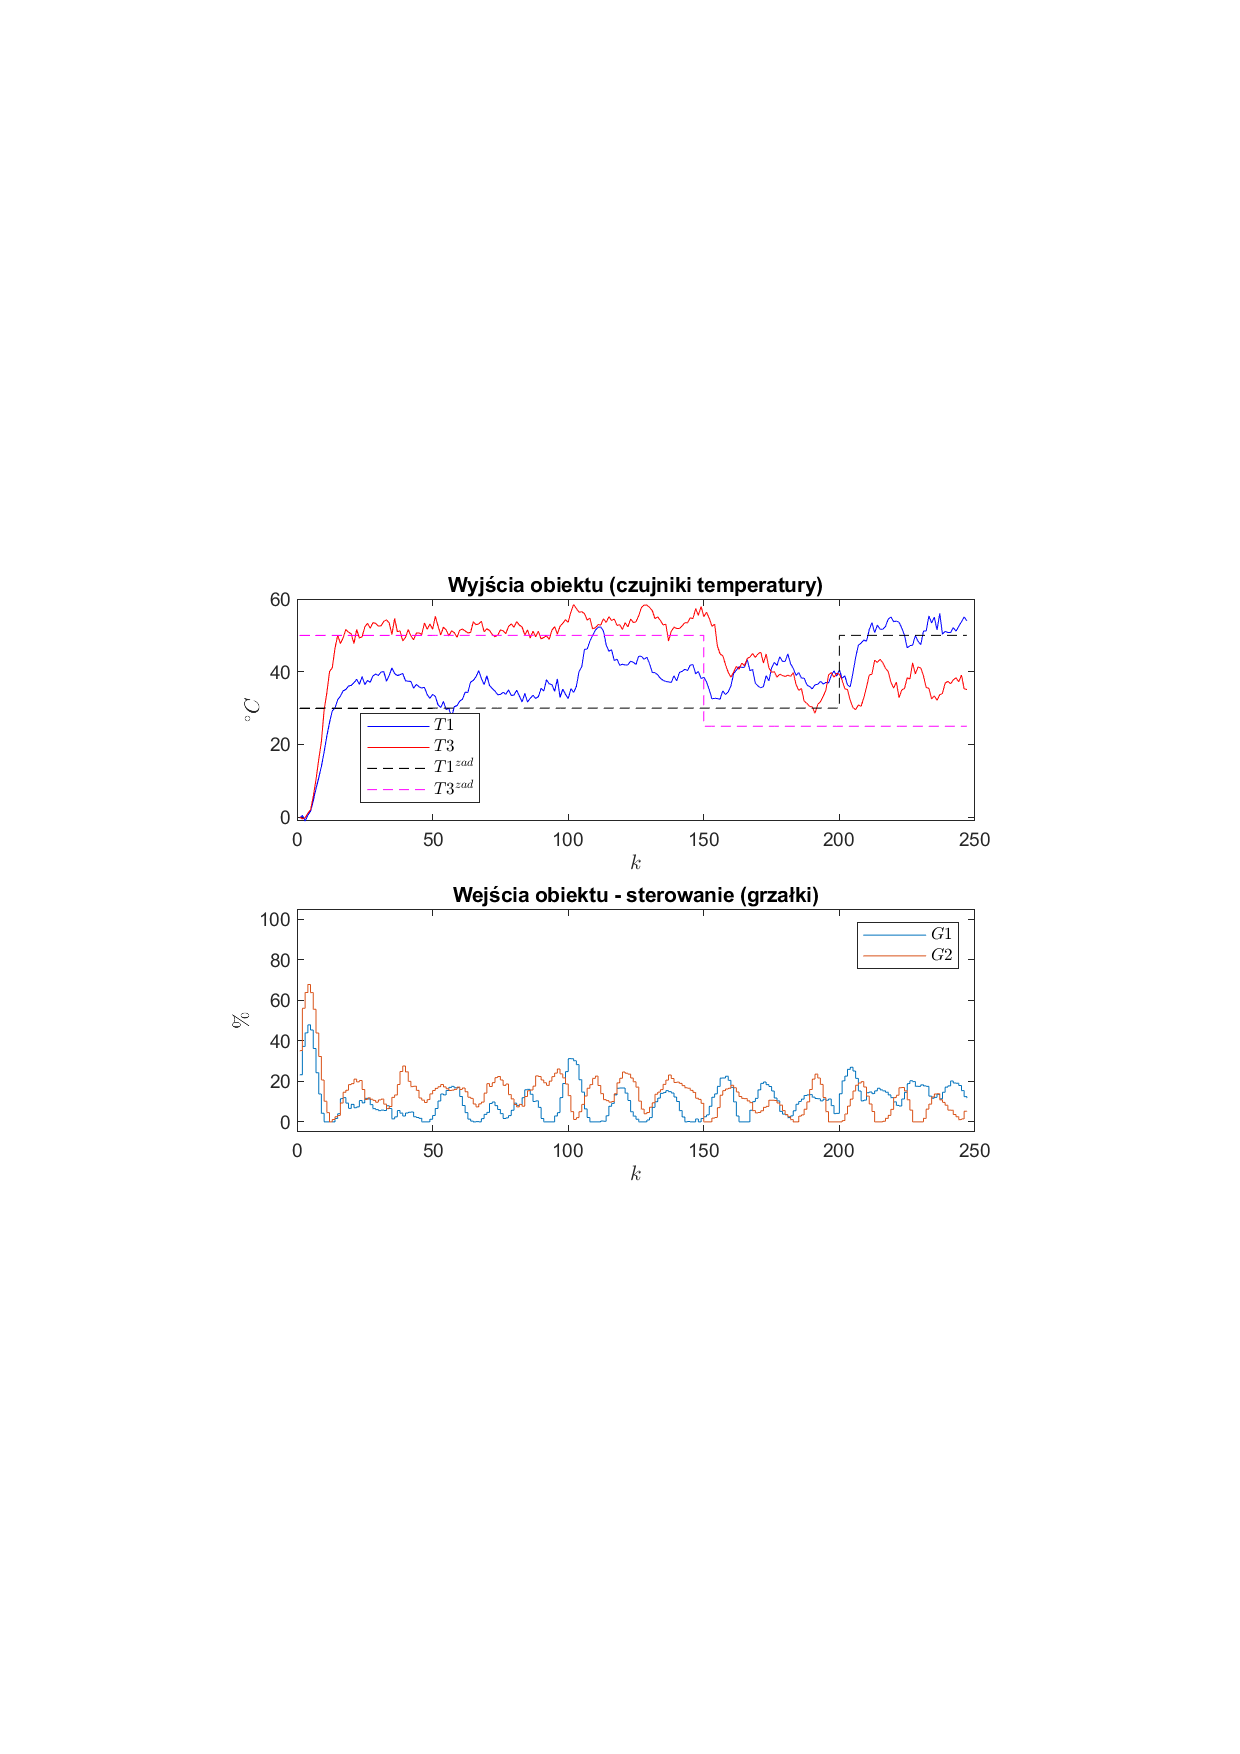
\includegraphics[scale=0.85, trim={2cm 8.5cm 2cm 8.5cm}]{rysunki/dmc_lambda1}
	\caption{Symulacja procesu dla $\lambda=1$}
	\label{dmc_lambda1}
\end{figure}


\begin{figure}
	\centering
	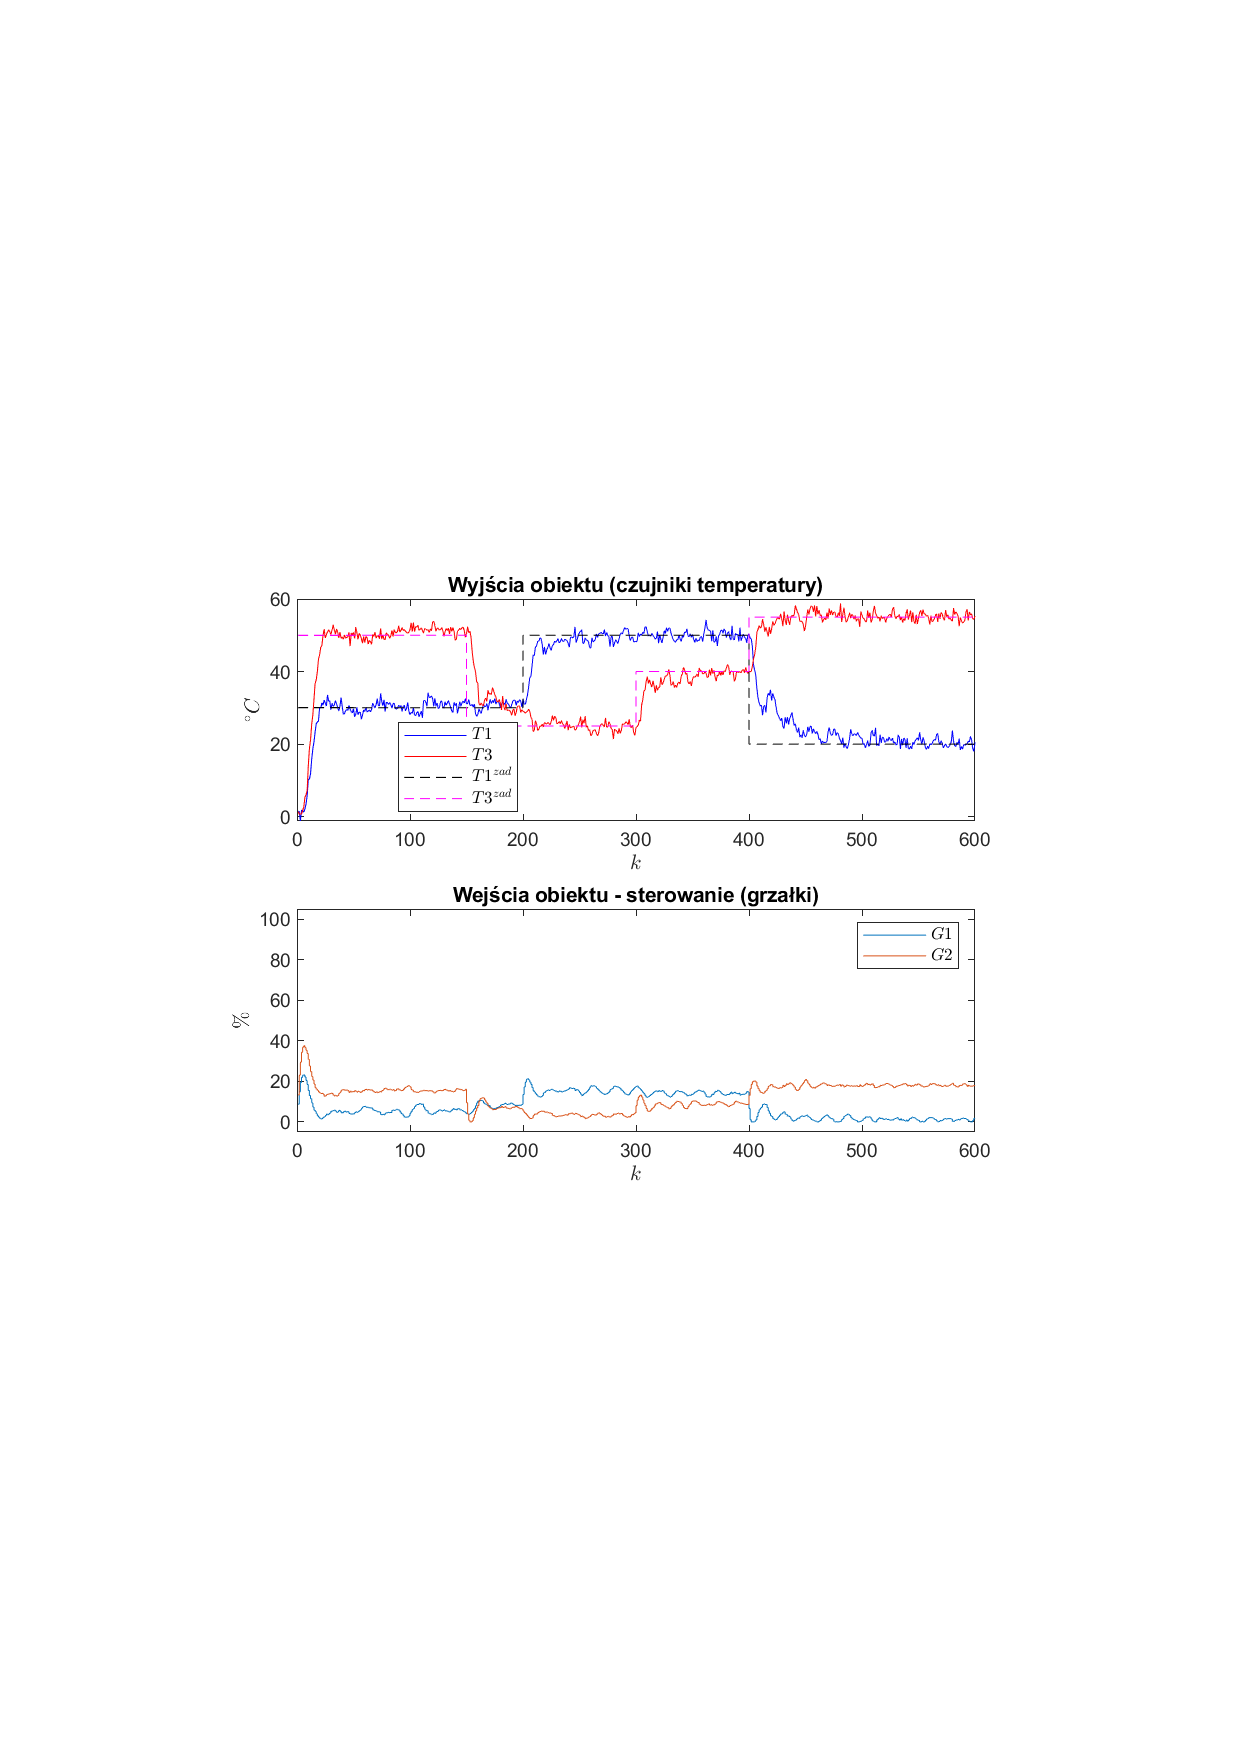
\includegraphics[scale=0.85, trim={2cm 8.5cm 2cm 8.5cm}]{rysunki/dmc_lambda10}
	\caption{Symulacja procesu dla $\lambda=10$}
	\label{dmc_lambda10}
\end{figure}

Ostatecznie przyj�li�my nast�puj�ce nastawy regulatora DMC

\begin{equation}
\label{dmc_final}
N=20, N_\mathrm{u}=3, \lambda=10
\end{equation}

Parametry te zapewni�y poprawn� prac� regulatora. 


\section{Implementacja}
Do kalibracji oraz symulacji algorytmu DMC wykorzystali�my skrypt \verb+DMC_MIMO.m+

\chapter{Dob�r nastaw regulator�w}

\section{Dob�r nastaw cyfrowego regulatora PID}
Nastawy regulatora PID dobrane zosta�y metod� in�yniersk�. Po przeprowadzeniu strojenia metod� in�yniersk� nastawy regulatora zosta�y dodatkowo poprawione tak, aby zminimalizowa� wska�nik jako�ci. Wska�nik jako�ci regulacji, wyznaczany za pomoc� metody najmniejszych kwadrat�w, dany jest wzorem:

\begin{equation}
E=\sum^{k_{\mathrm{konc}}}_{k=1}(y^{\mathrm{zad}}(k)-y(k))^2
\end{equation}

Na pocz�tku, przy w��czonym cz�onie proporcjonalnym P oraz wy��czonymi cz�onami ca�kuj�cym i r�niczkuj�cym uk�ad doprowadzony zosta� na granic� stabilno�ci poprzez takie dobranie wzmocnienia $K$, �e uk�ad wpad� w niegasn�ce oscylacje.

\begin{figure}[h!]
\centering
% This file was created by matlab2tikz.
%
%The latest updates can be retrieved from
%  http://www.mathworks.com/matlabcentral/fileexchange/22022-matlab2tikz-matlab2tikz
%where you can also make suggestions and rate matlab2tikz.
%
\definecolor{mycolor1}{rgb}{0.00000,0.44700,0.74100}%
\definecolor{mycolor2}{rgb}{0.85000,0.32500,0.09800}%
%
\begin{tikzpicture}[scale=0.8]

\begin{axis}[%
width=4.521in,
height=1.488in,
at={(0.758in,2.554in)},
scale only axis,
xmin=0,
xmax=800,
ymin=0.9,
ymax=1.3,
axis background/.style={fill=white},
title style={font=\bfseries},
title={Sygnal wejsciowy},
legend style={at={(0.97,0.03)}, anchor=south east, legend cell align=left, align=left, draw=white!15!black}
]
\addplot[const plot, color=mycolor1] table[row sep=crcr] {%
1	1.1\\
2	1.1\\
3	1.1\\
4	1.1\\
5	1.1\\
6	1.1\\
7	1.1\\
8	1.1\\
9	1.1\\
10	1.1\\
11	1.1\\
12	1.1\\
13	1.1\\
14	1.1\\
15	1.1\\
16	1.1\\
17	1.1\\
18	1.1\\
19	1.1\\
20	1.15\\
21	1.149999883\\
22	1.149999886\\
23	1.149999889\\
24	1.149999892\\
25	1.149999895\\
26	1.149999898\\
27	1.149999901\\
28	1.149999904\\
29	1.149999907\\
30	1.14899070979564\\
31	1.14617878402454\\
32	1.14185826465065\\
33	1.13628745166449\\
34	1.12969271765655\\
35	1.12227201032914\\
36	1.11419799296845\\
37	1.10562085904896\\
38	1.09667085360329\\
39	1.08746053079267\\
40	1.07810714392588\\
41	1.06876648566898\\
42	1.05963522349007\\
43	1.05093257941094\\
44	1.0428860115561\\
45	1.03572022632079\\
46	1.02964894748214\\
47	1.0248689531002\\
48	1.02155596427634\\
49	1.01986203316951\\
50	1.0199137212201\\
51	1.02180984698136\\
52	1.02561819026711\\
53	1.03137165839358\\
54	1.03906465959769\\
55	1.04865016941342\\
56	1.06003777768675\\
57	1.07309285527102\\
58	1.08763687049965\\
59	1.10344880818719\\
60	1.12026759977272\\
61	1.1377954745999\\
62	1.1557021797359\\
63	1.1736300492245\\
64	1.19119990744077\\
65	1.2080177704717\\
66	1.22368227702881\\
67	1.23779274508176\\
68	1.24995771788572\\
69	1.25980383677238\\
70	1.26698485956169\\
71	1.27119063246141\\
72	1.27215581798647\\
73	1.26966817952447\\
74	1.26357622346677\\
75	1.25379600232391\\
76	1.24031688764624\\
77	1.22320613072751\\
78	1.20261204267957\\
79	1.17876564391316\\
80	1.15198065636303\\
81	1.12265173964103\\
82	1.09125090413609\\
83	1.05832206923672\\
84	1.02447377263262\\
85	0.990370076365512\\
86	0.956719756245306\\
87	0.924263902697566\\
88	0.9\\
89	0.9\\
90	0.9\\
91	0.9\\
92	0.9\\
93	0.9\\
94	0.9\\
95	0.902662880600467\\
96	0.912093858563612\\
97	0.928493220339047\\
98	0.95179928628292\\
99	0.981271002569295\\
100	1.0157796833161\\
101	1.05433879015018\\
102	1.09608820643618\\
103	1.14028014453223\\
104	1.18626652237044\\
105	1.23343391421143\\
106	1.28106831642198\\
107	1.3\\
108	1.3\\
109	1.3\\
110	1.3\\
111	1.3\\
112	1.3\\
113	1.3\\
114	1.3\\
115	1.3\\
116	1.29704042115281\\
117	1.28516707860848\\
118	1.26546030922668\\
119	1.23924448858182\\
120	1.20768089997467\\
121	1.17178559569965\\
122	1.13244541370577\\
123	1.09043233392441\\
124	1.04641634043623\\
125	1.0009769393725\\
126	0.954673203893615\\
127	0.908220145476257\\
128	0.9\\
129	0.9\\
130	0.9\\
131	0.9\\
132	0.9\\
133	0.9\\
134	0.9\\
135	0.9\\
136	0.9\\
137	0.907112120706175\\
138	0.922890134801366\\
139	0.946063101541346\\
140	0.97535253888806\\
141	1.00963843760898\\
142	1.04794185415765\\
143	1.08940930414072\\
144	1.13329877636225\\
145	1.17896720508768\\
146	1.22585925408283\\
147	1.27335372928552\\
148	1.3\\
149	1.3\\
150	1.3\\
151	1.3\\
152	1.3\\
153	1.3\\
154	1.3\\
155	1.3\\
156	1.3\\
157	1.29804364015302\\
158	1.2870734744963\\
159	1.26803231439621\\
160	1.24227689337013\\
161	1.21099715323662\\
162	1.17523449623834\\
163	1.13589815297189\\
164	1.09377985433379\\
165	1.04956697717756\\
166	1.00385431675738\\
167	0.957194111195739\\
168	0.910278964275623\\
169	0.9\\
170	0.9\\
171	0.9\\
172	0.9\\
173	0.9\\
174	0.9\\
175	0.9\\
176	0.9\\
177	0.9\\
178	0.906054953413794\\
179	0.920856508360525\\
180	0.943166679383094\\
181	0.971694866903181\\
182	1.00531017688703\\
183	1.04302389173613\\
184	1.08397375363561\\
185	1.12740987920157\\
186	1.17268214203777\\
187	1.21922887582396\\
188	1.26644455181846\\
189	1.3\\
190	1.3\\
191	1.3\\
192	1.3\\
193	1.3\\
194	1.3\\
195	1.3\\
196	1.3\\
197	1.3\\
198	1.29902513574564\\
199	1.28898597760552\\
200	1.2706954104152\\
201	1.2455332263047\\
202	1.21470985818067\\
203	1.17928489940715\\
204	1.14018371240511\\
205	1.09821231704714\\
206	1.05407073092261\\
207	1.00836491669953\\
208	0.961637153250824\\
209	0.914554352245934\\
210	0.9\\
211	0.9\\
212	0.9\\
213	0.9\\
214	0.9\\
215	0.9\\
216	0.9\\
217	0.9\\
218	0.9\\
219	0.905003728730561\\
220	0.918827684612735\\
221	0.940310255002789\\
222	0.968142927118701\\
223	1.00117882748766\\
224	1.03841499470179\\
225	1.07897648433946\\
226	1.12210212295407\\
227	1.16713174600585\\
228	1.21349477079137\\
229	1.26059897475996\\
230	1.3\\
231	1.3\\
232	1.3\\
233	1.3\\
234	1.3\\
235	1.3\\
236	1.3\\
237	1.3\\
238	1.3\\
239	1.3\\
240	1.29093278953925\\
241	1.27344867194074\\
242	1.24894786276474\\
243	1.21865897948221\\
244	1.18365779250791\\
245	1.14488404201938\\
246	1.10315651372461\\
247	1.05918654769652\\
248	1.01359013734526\\
249	0.966898760198548\\
250	0.919752080861852\\
251	0.9\\
252	0.9\\
253	0.9\\
254	0.9\\
255	0.9\\
256	0.9\\
257	0.9\\
258	0.9\\
259	0.9\\
260	0.903925745497713\\
261	0.916744533331096\\
262	0.937389029636467\\
263	0.964530248644428\\
264	0.997003080810028\\
265	1.03378833483634\\
266	1.07399663490724\\
267	1.11685398775735\\
268	1.1616888524212\\
269	1.20792056187935\\
270	1.25496972334917\\
271	1.3\\
272	1.3\\
273	1.3\\
274	1.3\\
275	1.3\\
276	1.3\\
277	1.3\\
278	1.3\\
279	1.3\\
280	1.3\\
281	1.29194625322752\\
282	1.27531082192291\\
283	1.25151397341224\\
284	1.22180219296803\\
285	1.18726715972314\\
286	1.14886276593223\\
287	1.10742037495923\\
288	1.063662494087\\
289	1.01821502100792\\
290	0.971618207280483\\
291	0.924499024826893\\
292	0.9\\
293	0.9\\
294	0.9\\
295	0.9\\
296	0.9\\
297	0.9\\
298	0.9\\
299	0.9\\
300	0.9\\
301	0.902995079732831\\
302	0.914936671801092\\
303	0.934845292843478\\
304	0.961374809258102\\
305	0.993344828833792\\
306	1.0297225508621\\
307	1.06960649059819\\
308	1.11221189080981\\
309	1.15685765156926\\
310	1.20295462598156\\
311	1.24993469178112\\
312	1.29707372283401\\
313	1.3\\
314	1.3\\
315	1.3\\
316	1.3\\
317	1.3\\
318	1.3\\
319	1.3\\
320	1.3\\
321	1.3\\
322	1.29288295431398\\
323	1.27708537869951\\
324	1.25398166295237\\
325	1.22483622665946\\
326	1.19075671353454\\
327	1.15271121442322\\
328	1.11154370865791\\
329	1.06798790186502\\
330	1.02267962088354\\
331	0.976167910706636\\
332	0.92906861461176\\
333	0.9\\
334	0.9\\
335	0.9\\
336	0.9\\
337	0.9\\
338	0.9\\
339	0.9\\
340	0.9\\
341	0.9\\
342	0.902085826317027\\
343	0.913170059652958\\
344	0.932357799997861\\
345	0.958286416667199\\
346	0.989760811534446\\
347	1.0257350850282\\
348	1.06529609482934\\
349	1.10764871819721\\
350	1.15210264746244\\
351	1.19806056491864\\
352	1.24496545809975\\
353	1.29211852413194\\
354	1.3\\
355	1.3\\
356	1.3\\
357	1.3\\
358	1.3\\
359	1.3\\
360	1.3\\
361	1.3\\
362	1.3\\
363	1.29383883099093\\
364	1.27893310914697\\
365	1.25656692684153\\
366	1.22802383698067\\
367	1.19442851468689\\
368	1.15676419775433\\
369	1.11588832369785\\
370	1.07254654364805\\
371	1.02738527567297\\
372	0.980962944174269\\
373	0.93388439467247\\
374	0.9\\
375	0.9\\
376	0.9\\
377	0.9\\
378	0.9\\
379	0.9\\
380	0.9\\
381	0.9\\
382	0.9\\
383	0.901125326794353\\
384	0.91130356731321\\
385	0.929729005216084\\
386	0.955021661482761\\
387	0.985970972192122\\
388	1.02151726107176\\
389	1.06073512402551\\
390	1.10281853466629\\
391	1.14706749869323\\
392	1.19287610181063\\
393	1.23969909751526\\
394	1.28686446556351\\
395	1.3\\
396	1.3\\
397	1.3\\
398	1.3\\
399	1.3\\
400	1.3\\
401	1.3\\
402	1.3\\
403	1.3\\
404	1.29484863270342\\
405	1.28088513439857\\
406	1.25929782812571\\
407	1.23139053046627\\
408	1.19830595357671\\
409	1.16104337602889\\
410	1.12047448719237\\
411	1.07735758768847\\
412	1.03235031053302\\
413	0.986021011455193\\
414	0.93896293752663\\
415	0.9\\
416	0.9\\
417	0.9\\
418	0.9\\
419	0.9\\
420	0.9\\
421	0.9\\
422	0.9\\
423	0.9\\
424	0.90011018564968\\
425	0.909330921894681\\
426	0.926950531054509\\
427	0.951570728883698\\
428	0.98196463224496\\
429	1.01705802760006\\
430	1.05591257181262\\
431	1.09771073228464\\
432	1.14174229247405\\
433	1.1873922658721\\
434	1.23412785291761\\
435	1.28130534907045\\
436	1.3\\
437	1.3\\
438	1.3\\
439	1.3\\
440	1.3\\
441	1.3\\
442	1.3\\
443	1.3\\
444	1.3\\
445	1.29591577176967\\
446	1.28294801566831\\
447	1.26218371612691\\
448	1.23494812191623\\
449	1.20240302214536\\
450	1.16556466080375\\
451	1.12531980046011\\
452	1.0824401200574\\
453	1.03759511357524\\
454	0.991363639992678\\
455	0.944326696304258\\
456	0.9\\
457	0.9\\
458	0.9\\
459	0.9\\
460	0.9\\
461	0.9\\
462	0.9\\
463	0.9\\
464	0.9\\
465	0.9\\
466	0.908208724188684\\
467	0.924976566258498\\
468	0.948885905056884\\
469	0.978692618350115\\
470	1.01330713577541\\
471	1.05177744558254\\
472	1.09327386006826\\
473	1.1370753638586\\
474	1.18255738640792\\
475	1.2291808556348\\
476	1.27631671874072\\
477	1.3\\
478	1.3\\
479	1.3\\
480	1.3\\
481	1.3\\
482	1.3\\
483	1.3\\
484	1.3\\
485	1.3\\
486	1.29686377714773\\
487	1.28478887344902\\
488	1.26476996968545\\
489	1.23815034564196\\
490	1.20610785315176\\
491	1.16967303356165\\
492	1.12974536409233\\
493	1.08710782003384\\
494	1.04243992133465\\
495	0.996329415632435\\
496	0.949346036393659\\
497	0.902217747371148\\
498	0.9\\
499	0.9\\
500	0.9\\
501	0.9\\
502	0.9\\
503	0.9\\
504	0.9\\
505	0.9\\
506	0.9\\
507	0.907266438335896\\
508	0.923203219551172\\
509	0.946423128844637\\
510	0.975664561403643\\
511	1.00982238098107\\
512	1.04793072857467\\
513	1.0891476095931\\
514	1.13274108171809\\
515	1.17807688308307\\
516	1.22460735610848\\
517	1.27171487071446\\
518	1.3\\
519	1.3\\
520	1.3\\
521	1.3\\
522	1.3\\
523	1.3\\
524	1.3\\
525	1.3\\
526	1.3\\
527	1.29776562155363\\
528	1.28654116503884\\
529	1.26723607829006\\
530	1.2412102051842\\
531	1.20965616071784\\
532	1.17361763373232\\
533	1.13400580006001\\
534	1.09161403485483\\
535	1.04713109429393\\
536	1.00115292016984\\
537	0.954238304538237\\
538	0.907090159901287\\
539	0.9\\
540	0.9\\
541	0.9\\
542	0.9\\
543	0.9\\
544	0.9\\
545	0.9\\
546	0.9\\
547	0.9\\
548	0.906317725000228\\
549	0.921369462322235\\
550	0.943856726046771\\
551	0.972499042901443\\
552	1.00617447966937\\
553	1.04390223764006\\
554	1.08482704697602\\
555	1.12820518108779\\
556	1.17339192874478\\
557	1.21983037755283\\
558	1.26691385980819\\
559	1.3\\
560	1.3\\
561	1.3\\
562	1.3\\
563	1.3\\
564	1.3\\
565	1.3\\
566	1.3\\
567	1.3\\
568	1.29871784262817\\
569	1.28839164040049\\
570	1.26984190442003\\
571	1.24444574906249\\
572	1.21341118485001\\
573	1.1777956138961\\
574	1.13852241656345\\
575	1.09639581999251\\
576	1.05211422038041\\
577	1.00628211405889\\
578	0.959446656283955\\
579	0.912284230299773\\
580	0.9\\
581	0.9\\
582	0.9\\
583	0.9\\
584	0.9\\
585	0.9\\
586	0.9\\
587	0.9\\
588	0.9\\
589	0.905316366417645\\
590	0.919433802339311\\
591	0.94114847678854\\
592	0.969159865029389\\
593	1.00232818523906\\
594	1.03965676506062\\
595	1.08027623087298\\
596	1.12343033761791\\
597	1.1684632748976\\
598	1.21480830115377\\
599	1.26187026672081\\
600	1.3\\
601	1.3\\
602	1.3\\
603	1.3\\
604	1.3\\
605	1.3\\
606	1.3\\
607	1.3\\
608	1.3\\
609	1.29972411577134\\
610	1.29034707801527\\
611	1.27259599695653\\
612	1.24786615752876\\
613	1.2173817691037\\
614	1.18221466354313\\
615	1.14330106427334\\
616	1.10145661903131\\
617	1.05738986994155\\
618	1.01171431757941\\
619	0.964964788764517\\
620	0.917789606331079\\
621	0.9\\
622	0.9\\
623	0.9\\
624	0.9\\
625	0.9\\
626	0.9\\
627	0.9\\
628	0.9\\
629	0.9\\
630	0.904258457950178\\
631	0.917388780204065\\
632	0.938287487378449\\
633	0.965632822999881\\
634	0.998266106552849\\
635	1.03517385863636\\
636	1.07547177299156\\
637	1.11839035085358\\
638	1.16326203120751\\
639	1.209509666832\\
640	1.25655025801091\\
641	1.3\\
642	1.3\\
643	1.3\\
644	1.3\\
645	1.3\\
646	1.3\\
647	1.3\\
648	1.3\\
649	1.3\\
650	1.3\\
651	1.29162610294374\\
652	1.27471926772244\\
653	1.25069395539007\\
654	1.22079147096219\\
655	1.18609887523193\\
656	1.1475659463073\\
657	1.10602038562032\\
658	1.06218144394346\\
659	1.0166721257651\\
660	0.970030114851364\\
661	0.922886568570101\\
662	0.9\\
663	0.9\\
664	0.9\\
665	0.9\\
666	0.9\\
667	0.9\\
668	0.9\\
669	0.9\\
670	0.9\\
671	0.903287603356344\\
672	0.915505261855707\\
673	0.935643524314991\\
674	0.962361965122687\\
675	0.994485275392374\\
676	1.0309851775646\\
677	1.07096420791288\\
678	1.11364118032989\\
679	1.15833816311752\\
680	1.20446881698786\\
681	1.25146160037362\\
682	1.29858436904073\\
683	1.3\\
684	1.3\\
685	1.3\\
686	1.3\\
687	1.3\\
688	1.3\\
689	1.3\\
690	1.3\\
691	1.3\\
692	1.29257410947294\\
693	1.27648862418223\\
694	1.25314534351713\\
695	1.22380274568271\\
696	1.18956318308467\\
697	1.15139003822965\\
698	1.11012310468019\\
699	1.06649237050527\\
700	1.02113036429337\\
701	0.974583208105269\\
702	0.927470391774555\\
703	0.9\\
704	0.9\\
705	0.9\\
706	0.9\\
707	0.9\\
708	0.9\\
709	0.9\\
710	0.9\\
711	0.9\\
712	0.902394025283737\\
713	0.913769106755949\\
714	0.93320069419823\\
715	0.959331865556576\\
716	0.990972610127016\\
717	1.0270815584864\\
718	1.06674959874601\\
719	1.10918519068633\\
720	1.15370120787298\\
721	1.19970315449373\\
722	1.24663029767345\\
723	1.29377528533985\\
724	1.3\\
725	1.3\\
726	1.3\\
727	1.3\\
728	1.3\\
729	1.3\\
730	1.3\\
731	1.3\\
732	1.3\\
733	1.2935142967055\\
734	1.27830584637548\\
735	1.25568889881709\\
736	1.22694057926377\\
737	1.1931798405383\\
738	1.15538483057656\\
739	1.11440846383957\\
740	1.07099237614517\\
741	1.02577942485595\\
742	0.979324880489216\\
743	0.932237348939481\\
744	0.9\\
745	0.9\\
746	0.9\\
747	0.9\\
748	0.9\\
749	0.9\\
750	0.9\\
751	0.9\\
752	0.9\\
753	0.901450823880793\\
754	0.911936129600394\\
755	0.930619684127646\\
756	0.95612742787333\\
757	0.987254073510102\\
758	1.02294464460743\\
759	1.06227791965703\\
760	1.10445159116618\\
761	1.14876896823829\\
762	1.19462706786285\\
763	1.24147667188061\\
764	1.28863669655752\\
765	1.3\\
766	1.3\\
767	1.3\\
768	1.3\\
769	1.3\\
770	1.3\\
771	1.3\\
772	1.3\\
773	1.3\\
774	1.29450628135063\\
775	1.28022336740904\\
776	1.2583718730911\\
777	1.23024876911372\\
778	1.19699067375368\\
779	1.15959144589661\\
780	1.11891795941088\\
781	1.07572424060691\\
782	1.03066413271167\\
783	0.984302635224493\\
784	0.93723693674895\\
785	0.9\\
786	0.9\\
787	0.9\\
788	0.9\\
789	0.9\\
790	0.9\\
791	0.9\\
792	0.9\\
793	0.9\\
794	0.900454133085665\\
795	0.909999302304523\\
796	0.927891864582105\\
797	0.952739752016778\\
798	0.983321623203897\\
799	1.01856820105167\\
800	1.05754553600027\\
};
\addlegendentry{Sygnal sterujacy}

\end{axis}

\begin{axis}[%
width=4.521in,
height=1.488in,
at={(0.758in,0.481in)},
scale only axis,
xmin=0,
xmax=800,
ymin=1.8,
ymax=2.4,
axis background/.style={fill=white},
title style={font=\bfseries},
title={Sygnal wyjsciowy i zadany},
legend style={at={(0.97,0.03)}, anchor=south east, legend cell align=left, align=left, draw=white!15!black}
]
\addplot [color=mycolor1]
  table[row sep=crcr]{%
1	2\\
2	2\\
3	2\\
4	2\\
5	2\\
6	2\\
7	2\\
8	2\\
9	2\\
10	2\\
11	2\\
12	2\\
13	2\\
14	2\\
15	2\\
16	2\\
17	2\\
18	2\\
19	2\\
20	2\\
21	2\\
22	2\\
23	2\\
24	2\\
25	2\\
26	2\\
27	2\\
28	2\\
29	2\\
30	2.0005046\\
31	2.00191056419924\\
32	2.00407082522037\\
33	2.0068562330611\\
34	2.01015360142016\\
35	2.01386395644122\\
36	2.01790096647682\\
37	2.02218953478603\\
38	2.02666453884944\\
39	2.03126970158388\\
40	2.03594639633493\\
41	2.04061672677325\\
42	2.04518235916915\\
43	2.04953368251478\\
44	2.05355696775008\\
45	2.05713986167907\\
46	2.06017550241456\\
47	2.06256550092781\\
48	2.06422199666947\\
49	2.06506896356156\\
50	2.06504312088555\\
51	2.06409505936652\\
52	2.06219088909915\\
53	2.05931415642666\\
54	2.0554676572316\\
55	2.05067490374764\\
56	2.04498110105204\\
57	2.03845356371807\\
58	2.03118155757856\\
59	2.02327559022544\\
60	2.014866195938\\
61	2.0061022600429\\
62	1.99714890900465\\
63	1.98818497579914\\
64	1.97940004823624\\
65	1.9709911182696\\
66	1.96315886654033\\
67	1.95610363406029\\
68	1.95002114919845\\
69	1.94509809128544\\
70	1.94150758140776\\
71	1.93940469645809\\
72	1.93892210517569\\
73	1.94016592586368\\
74	1.94321190532366\\
75	1.94810201729798\\
76	1.95484157600957\\
77	1.96339695581017\\
78	1.97369400114308\\
79	1.98561720180277\\
80	1.99900969682241\\
81	2.01367415639731\\
82	2.02937457533497\\
83	2.04583899394382\\
84	2.06276314338242\\
85	2.07981499263399\\
86	2.09664015379829\\
87	2.11286808166783\\
88	2.12811898297092\\
89	2.14201133064103\\
90	2.15416985945991\\
91	2.16423390188582\\
92	2.17186590728774\\
93	2.17675997461784\\
94	2.1786502181967\\
95	2.17731877915088\\
96	2.17260329147131\\
97	2.16440361193791\\
98	2.15275058036376\\
99	2.13801472361022\\
100	2.12076038459358\\
101	2.10148083252598\\
102	2.08060612574679\\
103	2.05851015809523\\
104	2.0355169706205\\
105	2.01193327619948\\
106	1.98811607664078\\
107	1.96450394985206\\
108	1.9416031055296\\
109	1.91996580637943\\
110	1.90016141953692\\
111	1.88274954029655\\
112	1.86825993520704\\
113	1.85717808921677\\
114	1.84993532391517\\
115	1.84690206919217\\
116	1.84838185997494\\
117	1.85431853259898\\
118	1.86417191871031\\
119	1.87727983052821\\
120	1.89306162637115\\
121	1.91100928006531\\
122	1.93067937261354\\
123	1.95168591403102\\
124	1.97369391226137\\
125	1.99641361422562\\
126	2.01956548333869\\
127	2.04279201387654\\
128	2.06562596834066\\
129	2.08753379058205\\
130	2.10795344790218\\
131	2.12632361690635\\
132	2.14210569380979\\
133	2.15479989255787\\
134	2.1639565057778\\
135	2.1691832406048\\
136	2.17015000348809\\
137	2.16659394469771\\
138	2.15870493920346\\
139	2.14711845730841\\
140	2.13247374004771\\
141	2.11533079206739\\
142	2.09617908516603\\
143	2.07544536156184\\
144	2.05350062687091\\
145	2.03066641397567\\
146	2.00722039100574\\
147	1.98347315498791\\
148	1.9598448372025\\
149	1.9368476986073\\
150	1.91504378420472\\
151	1.89501029795595\\
152	1.87731313623074\\
153	1.8624871671707\\
154	1.85102205206533\\
155	1.84335258560084\\
156	1.83985268814815\\
157	1.84083086947432\\
158	1.84631595368343\\
159	1.85583653517099\\
160	1.86871424720123\\
161	1.88435411883288\\
162	1.90223544891725\\
163	1.92190362213276\\
164	1.94296277301145\\
165	1.96506921311003\\
166	1.98792554478765\\
167	2.01125564897577\\
168	2.03471322379541\\
169	2.05783683658359\\
170	2.08009314359987\\
171	2.10091618750703\\
172	2.11973777203276\\
173	2.13601043536632\\
174	2.1492243208907\\
175	2.15891905060928\\
176	2.16469153938452\\
177	2.16620094210187\\
178	2.16317346697891\\
179	2.15577269108284\\
180	2.14461760707144\\
181	2.13035351474577\\
182	2.11354586115281\\
183	2.09468900511751\\
184	2.07421407556913\\
185	2.052496014218\\
186	2.02985988427763\\
187	2.00658651892086\\
188	1.98297868251659\\
189	1.95944080342177\\
190	1.93647407057408\\
191	1.91463363768189\\
192	1.8944931733659\\
193	1.87661769869444\\
194	1.8615432817327\\
195	1.84976236970869\\
196	1.84171372214798\\
197	1.83777606638277\\
198	1.83826349993483\\
199	1.8432830803946\\
200	1.85242836542534\\
201	1.86500945899983\\
202	1.88042114463215\\
203	1.89813362561237\\
204	1.91768422070622\\
205	1.9386699199573\\
206	1.96074071455402\\
207	1.9835936231483\\
208	2.00695750629408\\
209	2.03049890816738\\
210	2.05376465798273\\
211	2.07622473470319\\
212	2.09731272918535\\
213	2.11645718030911\\
214	2.13310533688228\\
215	2.14674067008237\\
216	2.15689526439579\\
217	2.16315804466371\\
218	2.1651798481992\\
219	2.16267798541901\\
220	2.15576600906384\\
221	2.14502472538269\\
222	2.13110839076942\\
223	2.11459044199101\\
224	2.09597235977757\\
225	2.0756916163621\\
226	2.05412879848666\\
227	2.03161398843681\\
228	2.00843247757728\\
229	1.98488037718382\\
230	1.96134741410307\\
231	1.93832486349381\\
232	1.91636262762268\\
233	1.89603277041599\\
234	1.87790150875905\\
235	1.86250820570193\\
236	1.85035012493974\\
237	1.84187189151256\\
238	1.83745876419753\\
239	1.83743194445518\\
240	1.84196555107497\\
241	1.85070761130086\\
242	1.86295801740302\\
243	1.87810246061283\\
244	1.89560305569448\\
245	1.91498993253501\\
246	1.93585369825991\\
247	1.95783868281548\\
248	1.98063688948228\\
249	2.00398257948459\\
250	2.02755592052856\\
251	2.05091326600555\\
252	2.07352924412304\\
253	2.094838318218\\
254	2.11426703417042\\
255	2.13125853407579\\
256	2.14529068466076\\
257	2.15588896893261\\
258	2.16263511641199\\
259	2.16517229764006\\
260	2.16320942647026\\
261	2.15680003414285\\
262	2.14647778751454\\
263	2.13290717946177\\
264	2.11667076478819\\
265	2.0982781391689\\
266	2.07817399053462\\
267	2.05674531553718\\
268	2.03432788467532\\
269	2.01121203147208\\
270	1.98768745232167\\
271	1.96412912302972\\
272	1.94101854061716\\
273	1.91890079257081\\
274	1.8983469796818\\
275	1.87992528410073\\
276	1.8641792002417\\
277	1.85161166403711\\
278	1.84267400482666\\
279	1.83775880749292\\
280	1.83719511387586\\
281	1.84122198864794\\
282	1.84953970571517\\
283	1.86143813147692\\
284	1.8762940232632\\
285	1.89356154147868\\
286	1.91276373997139\\
287	1.93348493703847\\
288	1.95536387902091\\
289	1.97808761705786\\
290	2.00138602535796\\
291	2.02494561796669\\
292	2.0483359256935\\
293	2.07103940879388\\
294	2.09249416125795\\
295	2.11212711191934\\
296	2.12937932905121\\
297	2.14372480080589\\
298	2.15468386067788\\
299	2.16183225124239\\
300	2.1648066673282\\
301	2.16330912903589\\
302	2.15733833459479\\
303	2.14738402560849\\
304	2.13411926885951\\
305	2.11813426048508\\
306	2.0999454008665\\
307	2.08000343239921\\
308	2.05870073371878\\
309	2.0363778548054\\
310	2.0133293691201\\
311	1.98983933780071\\
312	1.96626982389989\\
313	1.94309361336248\\
314	1.920851358722\\
315	1.90011305493361\\
316	1.8814483199275\\
317	1.86540397431857\\
318	1.85248763565403\\
319	1.84315623405412\\
320	1.83780852178632\\
321	1.83678018236493\\
322	1.84033870659777\\
323	1.84823749581551\\
324	1.8597893551884\\
325	1.8743620748953\\
326	1.89140183304995\\
327	1.91042458420444\\
328	1.93100833867131\\
329	1.95278624361944\\
330	1.97544038561437\\
331	1.99869624214714\\
332	2.02224589158346\\
333	2.04567131843501\\
334	2.06846284206133\\
335	2.09006222075226\\
336	2.10989680651122\\
337	2.12740564032029\\
338	2.14205888417769\\
339	2.15337177982606\\
340	2.16091414536824\\
341	2.16431626642942\\
342	2.16327335484094\\
343	2.15773123977031\\
344	2.14813737114353\\
345	2.13517306427468\\
346	2.11943586825911\\
347	2.10144873291001\\
348	2.08166822941032\\
349	2.06049191915015\\
350	2.03826495598077\\
351	2.01528599876919\\
352	1.99183355375553\\
353	1.96825702236403\\
354	1.94502062115063\\
355	1.92266059124638\\
356	1.90174575720905\\
357	1.88284704465941\\
358	1.86651442877018\\
359	1.85326000958384\\
360	1.84354610420258\\
361	1.83777741384797\\
362	1.83629604403543\\
363	1.83937662993839\\
364	1.8468294922704\\
365	1.85801258491497\\
366	1.87228413140197\\
367	1.88908179414022\\
368	1.90791395420711\\
369	1.92835189282353\\
370	1.9500227844059\\
371	1.97260341990493\\
372	1.99581458710713\\
373	2.01935386325448\\
374	2.04281615510977\\
375	2.06570025989956\\
376	2.08745193032921\\
377	2.10749904752694\\
378	2.12527856049221\\
379	2.14025661388193\\
380	2.15194307618631\\
381	2.15990149864119\\
382	2.16375537807865\\
383	2.16319271624741\\
384	2.15810359759003\\
385	2.14889088019583\\
386	2.13624455353637\\
387	2.12076989960482\\
388	2.10299675656528\\
389	2.0833878264896\\
390	2.06234612259143\\
391	2.0402216420381\\
392	2.01731734199151\\
393	1.99390584571258\\
394	1.97032316331212\\
395	1.94702443744229\\
396	1.92454122236508\\
397	1.90344107656585\\
398	1.88429627636679\\
399	1.86766009906946\\
400	1.8540493511795\\
401	1.84393201406258\\
402	1.83771904972244\\
403	1.83575932737663\\
404	1.8383350124326\\
405	1.84531676299468\\
406	1.85611041761517\\
407	1.87006406799745\\
408	1.88660635803282\\
409	1.90523764840932\\
410	1.92552209442005\\
411	1.9470805457357\\
412	1.96958418583272\\
413	1.9927488368336\\
414	2.01627787520244\\
415	2.03977985100491\\
416	2.06276250806252\\
417	2.08467580490741\\
418	2.1049481650242\\
419	2.12301430944568\\
420	2.13833612057891\\
421	2.15041777274595\\
422	2.15881618006031\\
423	2.16314765235326\\
424	2.16309256109013\\
425	2.15848219457475\\
426	2.14967239156433\\
427	2.13736229413221\\
428	2.12216534388013\\
429	2.10461864760557\\
430	2.08519137690088\\
431	2.06429229808552\\
432	2.04227651944773\\
433	2.01945153425623\\
434	1.9960837423032\\
435	1.97249499584952\\
436	1.94913084174779\\
437	1.92651787249763\\
438	1.90522229865199\\
439	1.88581781345605\\
440	1.86886117340445\\
441	1.85487414871525\\
442	1.84433069739405\\
443	1.83764838942321\\
444	1.83518323457935\\
445	1.83722535011204\\
446	1.84370922957203\\
447	1.85409138081857\\
448	1.86770917947228\\
449	1.88398173094754\\
450	1.90240091322306\\
451	1.92252334499192\\
452	1.94396318676358\\
453	1.96638569153225\\
454	1.98950142979517\\
455	2.01301990305253\\
456	2.03656407654176\\
457	2.05965114529264\\
458	2.08173550755522\\
459	2.10224615410598\\
460	2.12061544517514\\
461	2.13630075247112\\
462	2.14880022656737\\
463	2.15766376171256\\
464	2.16250006729898\\
465	2.16298144652599\\
466	2.15887708604415\\
467	2.15049316659172\\
468	2.1385384986841\\
469	2.12363514347179\\
470	2.10632788616502\\
471	2.08709273266348\\
472	2.06634452683964\\
473	2.044443776398\\
474	2.02170276662603\\
475	1.9983910335765\\
476	1.97482310364174\\
477	1.95143154772657\\
478	1.92873522434245\\
479	1.9072967364778\\
480	1.88768936548032\\
481	1.87047187900578\\
482	1.85616984391134\\
483	1.84526227772336\\
484	1.83817264786261\\
485	1.8352633795774\\
486	1.83683149242782\\
487	1.84286894568406\\
488	1.85287839903207\\
489	1.86618821259608\\
490	1.88220946042789\\
491	1.90042687182713\\
492	1.92039070816046\\
493	1.94170948176346\\
494	1.96404343264564\\
495	1.98709868697463\\
496	2.01059037801251\\
497	2.03415452389741\\
498	2.05731706505726\\
499	2.079536745625\\
500	2.10024348554787\\
501	2.11886797394584\\
502	2.1348639854718\\
503	2.14772470098885\\
504	2.15699412285159\\
505	2.16227450978228\\
506	2.16323125237124\\
507	2.15959803481421\\
508	2.15162964579554\\
509	2.14001969264799\\
510	2.1253989778071\\
511	2.10832006942573\\
512	2.08926589703001\\
513	2.06865745793684\\
514	2.04686072332321\\
515	2.02419282413732\\
516	2.00092758918128\\
517	1.97737383349024\\
518	1.95395161966042\\
519	1.93117198644161\\
520	1.90959384800311\\
521	1.8897899924336\\
522	1.87232111380189\\
523	1.85771648527614\\
524	1.84646008666814\\
525	1.83898117805007\\
526	1.83564846524334\\
527	1.83676565589551\\
528	1.84237788555604\\
529	1.85203043038634\\
530	1.86504336847451\\
531	1.88082039229021\\
532	1.89883965738537\\
533	1.91864557582048\\
534	1.93984145999886\\
535	1.96208293181539\\
536	1.98507202036002\\
537	2.00852932959817\\
538	2.03210340329171\\
539	2.05532864116421\\
540	2.07766810574628\\
541	2.09855281063505\\
542	2.11741207578558\\
543	2.13369647400529\\
544	2.14689466941389\\
545	2.15654525500075\\
546	2.16224452883999\\
547	2.16365145886946\\
548	2.16049259797215\\
549	2.1529667309009\\
550	2.14172310054546\\
551	2.12740194356081\\
552	2.11056422658525\\
553	2.09170034899947\\
554	2.07123794574385\\
555	2.04954888013133\\
556	2.02695550779244\\
557	2.00373628493685\\
558	1.98019454541385\\
559	1.95673750738609\\
560	1.93386777237677\\
561	1.91214025675731\\
562	1.8921271837604\\
563	1.874391280874\\
564	1.85946576490376\\
565	1.84783990622317\\
566	1.83994914495551\\
567	1.83616888855583\\
568	1.83680996867503\\
569	1.84197307118751\\
570	1.85124794062233\\
571	1.86394601982847\\
572	1.87946330351235\\
573	1.89727109058937\\
574	1.91690769085448\\
575	1.93797099071742\\
576	1.96011179206276\\
577	1.98302784671062\\
578	2.00644557702407\\
579	2.03002679139228\\
580	2.05331487165019\\
581	2.07577750708115\\
582	2.09684694297079\\
583	2.11595113487229\\
584	2.13253735617339\\
585	2.14608958004549\\
586	2.15614076050961\\
587	2.16228096740599\\
588	2.1641624443592\\
589	2.16150426274414\\
590	2.15444554637354\\
591	2.14358821066356\\
592	2.12958251798988\\
593	2.11299835929429\\
594	2.0943340707812\\
595	2.07402433928322\\
596	2.05244728734804\\
597	2.02993082019013\\
598	2.00675830860153\\
599	1.98322732741474\\
600	1.95973155885973\\
601	1.9367647245982\\
602	1.91487755860027\\
603	1.89464173229106\\
604	1.87662216738875\\
605	1.86135629195378\\
606	1.8493390079747\\
607	1.84101232316631\\
608	1.83675875911323\\
609	1.83689670266511\\
610	1.84158522293683\\
611	1.85046076489868\\
612	1.86282568613148\\
613	1.87806788191632\\
614	1.89565143629403\\
615	1.91510823752738\\
616	1.93603046172746\\
617	1.95806383781488\\
618	1.98090161548765\\
619	2.00427638132475\\
620	2.02786397391856\\
621	2.05121728229364\\
622	2.07380890720713\\
623	2.09507242183708\\
624	2.1144343682682\\
625	2.13133856202081\\
626	2.14526404709511\\
627	2.1557378447991\\
628	2.16234346718006\\
629	2.16472607302406\\
630	2.16259684563303\\
631	2.1560316860967\\
632	2.14558233403231\\
633	2.13190966767253\\
634	2.11559302730609\\
635	2.09713915265994\\
636	2.07699019688604\\
637	2.05553090938579\\
638	2.03309507068257\\
639	2.00997125440026\\
640	1.98645096039904\\
641	1.9629135780655\\
642	1.93984345676259\\
643	1.91778692501102\\
644	1.8973150869259\\
645	1.87899519928702\\
646	1.8633691564283\\
647	1.85093782672009\\
648	1.8421501720781\\
649	1.83739624428291\\
650	1.83700242468626\\
651	1.84118937460276\\
652	1.84964279363303\\
653	1.86165545130913\\
654	1.87660669508969\\
655	1.89395299454942\\
656	1.91321946060977\\
657	1.93399224253396\\
658	1.95591171491829\\
659	1.97866637550399\\
660	2.00198738239596\\
661	2.02555915691757\\
662	2.04894695827953\\
663	2.07163062042098\\
664	2.09304691223333\\
665	2.11262245103116\\
666	2.12979876785735\\
667	2.14405088996011\\
668	2.15490060353148\\
669	2.16192538468411\\
670	2.16476383526059\\
671	2.16312003515916\\
672	2.15701120750216\\
673	2.14694207780469\\
674	2.13358285885755\\
675	2.11752120513543\\
676	2.099271255445\\
677	2.07928174167239\\
678	2.05794325689062\\
679	2.03559476696496\\
680	2.01252944155284\\
681	1.98903305144227\\
682	1.96547166873545\\
683	1.94232075777132\\
684	1.92012227805403\\
685	1.89944646834485\\
686	1.880862383104\\
687	1.86491568337822\\
688	1.85211240415589\\
689	1.84290761079288\\
690	1.83769802201659\\
691	1.83681714979992\\
692	1.84053009645132\\
693	1.84857284050796\\
694	1.86024448234268\\
695	1.87491578282206\\
696	1.892035565714\\
697	1.91112213974026\\
698	1.93175560809842\\
699	1.95357097673618\\
700	1.97625198134445\\
701	1.99952556088054\\
702	2.02308197043281\\
703	2.04649898163173\\
704	2.06926412926675\\
705	2.09081781502196\\
706	2.11058714129992\\
707	2.12801174004917\\
708	2.14256298491235\\
709	2.15375776970089\\
710	2.16116785840961\\
711	2.1644256582589\\
712	2.16322864718886\\
713	2.15754110804893\\
714	2.14782531587003\\
715	2.13475973165435\\
716	2.11893936078584\\
717	2.10088488800341\\
718	2.08105086927467\\
719	2.05983307472906\\
720	2.03757506760026\\
721	2.0145740958081\\
722	1.99111052579655\\
723	1.96753803358851\\
724	1.94432372040472\\
725	1.92200529220351\\
726	1.90115193329581\\
727	1.88233408569697\\
728	1.86610061400131\\
729	1.85296205844948\\
730	1.84337887203009\\
731	1.83775370462736\\
732	1.83642645400978\\
733	1.83966930705277\\
734	1.84727353362815\\
735	1.85858200890186\\
736	1.87295617023653\\
737	1.88983654119105\\
738	1.90873404777206\\
739	1.92922223272753\\
740	1.95093027813038\\
741	1.97353675528413\\
742	1.99676402891759\\
743	2.02030779608648\\
744	2.04375856553205\\
745	2.06661224319957\\
746	2.08831320685152\\
747	2.10828913560623\\
748	2.12597766456827\\
749	2.14084627779161\\
750	2.15240664418048\\
751	2.160224420231\\
752	2.16392538724822\\
753	2.16319997687528\\
754	2.15795732561604\\
755	2.14861554990581\\
756	2.13586167950419\\
757	2.12029835810729\\
758	2.10245307395815\\
759	2.08278643783451\\
760	2.06169960350276\\
761	2.03954091642798\\
762	2.01661186812939\\
763	1.99318706769516\\
764	1.96960705698076\\
765	1.9463300459806\\
766	1.9238891661515\\
767	1.90285239181071\\
768	1.8837915272785\\
769	1.86725871631795\\
770	1.85376915638623\\
771	1.84378889607709\\
772	1.83772676366149\\
773	1.83592932560441\\
774	1.83867618633372\\
775	1.84581764471436\\
776	1.85674339336007\\
777	1.87080494690273\\
778	1.88743399617365\\
779	1.90613361170416\\
780	1.92647035653808\\
781	1.9480672175017\\
782	1.97059727296602\\
783	1.99377802316853\\
784	2.01731087380816\\
785	2.04079974570941\\
786	2.06374934499978\\
787	2.08560819770529\\
788	2.10580453555988\\
789	2.1237738264316\\
790	2.13897938910168\\
791	2.15092731996071\\
792	2.15917677538931\\
793	2.16334649461828\\
794	2.16311942963864\\
795	2.15834684663465\\
796	2.14940056706123\\
797	2.13697662482348\\
798	2.12168569065666\\
799	2.10406240313488\\
800	2.08457373706206\\
};
\addlegendentry{Wyjscie procesu}

\addplot[const plot, color=mycolor2, dashed] table[row sep=crcr] {%
1	2\\
2	2\\
3	2\\
4	2\\
5	2\\
6	2\\
7	2\\
8	2\\
9	2\\
10	2\\
11	2\\
12	2\\
13	2\\
14	2\\
15	2\\
16	2\\
17	2\\
18	2\\
19	2\\
20	2.3\\
21	2.3\\
22	2.3\\
23	2.3\\
24	2.3\\
25	2.3\\
26	2.3\\
27	2.3\\
28	2.3\\
29	2.3\\
30	2.3\\
31	2.3\\
32	2.3\\
33	2.3\\
34	2.3\\
35	2.3\\
36	2.3\\
37	2.3\\
38	2.3\\
39	2.3\\
40	2.3\\
41	2.3\\
42	2.3\\
43	2.3\\
44	2.3\\
45	2.3\\
46	2.3\\
47	2.3\\
48	2.3\\
49	2.3\\
50	2.3\\
51	2.3\\
52	2.3\\
53	2.3\\
54	2.3\\
55	2.3\\
56	2.3\\
57	2.3\\
58	2.3\\
59	2.3\\
60	2.3\\
61	2.3\\
62	2.3\\
63	2.3\\
64	2.3\\
65	2.3\\
66	2.3\\
67	2.3\\
68	2.3\\
69	2.3\\
70	2.3\\
71	2.3\\
72	2.3\\
73	2.3\\
74	2.3\\
75	2.3\\
76	2.3\\
77	2.3\\
78	2.3\\
79	2.3\\
80	2.3\\
81	2.3\\
82	2.3\\
83	2.3\\
84	2.3\\
85	2.3\\
86	2.3\\
87	2.3\\
88	2.3\\
89	2.3\\
90	2.3\\
91	2.3\\
92	2.3\\
93	2.3\\
94	2.3\\
95	2.3\\
96	2.3\\
97	2.3\\
98	2.3\\
99	2.3\\
100	2.3\\
101	2.3\\
102	2.3\\
103	2.3\\
104	2.3\\
105	2.3\\
106	2.3\\
107	2.3\\
108	2.3\\
109	2.3\\
110	2.3\\
111	2.3\\
112	2.3\\
113	2.3\\
114	2.3\\
115	2.3\\
116	2.3\\
117	2.3\\
118	2.3\\
119	2.3\\
120	2.3\\
121	2.3\\
122	2.3\\
123	2.3\\
124	2.3\\
125	2.3\\
126	2.3\\
127	2.3\\
128	2.3\\
129	2.3\\
130	2.3\\
131	2.3\\
132	2.3\\
133	2.3\\
134	2.3\\
135	2.3\\
136	2.3\\
137	2.3\\
138	2.3\\
139	2.3\\
140	2.3\\
141	2.3\\
142	2.3\\
143	2.3\\
144	2.3\\
145	2.3\\
146	2.3\\
147	2.3\\
148	2.3\\
149	2.3\\
150	2.3\\
151	2.3\\
152	2.3\\
153	2.3\\
154	2.3\\
155	2.3\\
156	2.3\\
157	2.3\\
158	2.3\\
159	2.3\\
160	2.3\\
161	2.3\\
162	2.3\\
163	2.3\\
164	2.3\\
165	2.3\\
166	2.3\\
167	2.3\\
168	2.3\\
169	2.3\\
170	2.3\\
171	2.3\\
172	2.3\\
173	2.3\\
174	2.3\\
175	2.3\\
176	2.3\\
177	2.3\\
178	2.3\\
179	2.3\\
180	2.3\\
181	2.3\\
182	2.3\\
183	2.3\\
184	2.3\\
185	2.3\\
186	2.3\\
187	2.3\\
188	2.3\\
189	2.3\\
190	2.3\\
191	2.3\\
192	2.3\\
193	2.3\\
194	2.3\\
195	2.3\\
196	2.3\\
197	2.3\\
198	2.3\\
199	2.3\\
200	2.3\\
201	2.3\\
202	2.3\\
203	2.3\\
204	2.3\\
205	2.3\\
206	2.3\\
207	2.3\\
208	2.3\\
209	2.3\\
210	2.3\\
211	2.3\\
212	2.3\\
213	2.3\\
214	2.3\\
215	2.3\\
216	2.3\\
217	2.3\\
218	2.3\\
219	2.3\\
220	2.3\\
221	2.3\\
222	2.3\\
223	2.3\\
224	2.3\\
225	2.3\\
226	2.3\\
227	2.3\\
228	2.3\\
229	2.3\\
230	2.3\\
231	2.3\\
232	2.3\\
233	2.3\\
234	2.3\\
235	2.3\\
236	2.3\\
237	2.3\\
238	2.3\\
239	2.3\\
240	2.3\\
241	2.3\\
242	2.3\\
243	2.3\\
244	2.3\\
245	2.3\\
246	2.3\\
247	2.3\\
248	2.3\\
249	2.3\\
250	2.3\\
251	2.3\\
252	2.3\\
253	2.3\\
254	2.3\\
255	2.3\\
256	2.3\\
257	2.3\\
258	2.3\\
259	2.3\\
260	2.3\\
261	2.3\\
262	2.3\\
263	2.3\\
264	2.3\\
265	2.3\\
266	2.3\\
267	2.3\\
268	2.3\\
269	2.3\\
270	2.3\\
271	2.3\\
272	2.3\\
273	2.3\\
274	2.3\\
275	2.3\\
276	2.3\\
277	2.3\\
278	2.3\\
279	2.3\\
280	2.3\\
281	2.3\\
282	2.3\\
283	2.3\\
284	2.3\\
285	2.3\\
286	2.3\\
287	2.3\\
288	2.3\\
289	2.3\\
290	2.3\\
291	2.3\\
292	2.3\\
293	2.3\\
294	2.3\\
295	2.3\\
296	2.3\\
297	2.3\\
298	2.3\\
299	2.3\\
300	2.3\\
301	2.3\\
302	2.3\\
303	2.3\\
304	2.3\\
305	2.3\\
306	2.3\\
307	2.3\\
308	2.3\\
309	2.3\\
310	2.3\\
311	2.3\\
312	2.3\\
313	2.3\\
314	2.3\\
315	2.3\\
316	2.3\\
317	2.3\\
318	2.3\\
319	2.3\\
320	2.3\\
321	2.3\\
322	2.3\\
323	2.3\\
324	2.3\\
325	2.3\\
326	2.3\\
327	2.3\\
328	2.3\\
329	2.3\\
330	2.3\\
331	2.3\\
332	2.3\\
333	2.3\\
334	2.3\\
335	2.3\\
336	2.3\\
337	2.3\\
338	2.3\\
339	2.3\\
340	2.3\\
341	2.3\\
342	2.3\\
343	2.3\\
344	2.3\\
345	2.3\\
346	2.3\\
347	2.3\\
348	2.3\\
349	2.3\\
350	2.3\\
351	2.3\\
352	2.3\\
353	2.3\\
354	2.3\\
355	2.3\\
356	2.3\\
357	2.3\\
358	2.3\\
359	2.3\\
360	2.3\\
361	2.3\\
362	2.3\\
363	2.3\\
364	2.3\\
365	2.3\\
366	2.3\\
367	2.3\\
368	2.3\\
369	2.3\\
370	2.3\\
371	2.3\\
372	2.3\\
373	2.3\\
374	2.3\\
375	2.3\\
376	2.3\\
377	2.3\\
378	2.3\\
379	2.3\\
380	2.3\\
381	2.3\\
382	2.3\\
383	2.3\\
384	2.3\\
385	2.3\\
386	2.3\\
387	2.3\\
388	2.3\\
389	2.3\\
390	2.3\\
391	2.3\\
392	2.3\\
393	2.3\\
394	2.3\\
395	2.3\\
396	2.3\\
397	2.3\\
398	2.3\\
399	2.3\\
400	2.3\\
401	2.3\\
402	2.3\\
403	2.3\\
404	2.3\\
405	2.3\\
406	2.3\\
407	2.3\\
408	2.3\\
409	2.3\\
410	2.3\\
411	2.3\\
412	2.3\\
413	2.3\\
414	2.3\\
415	2.3\\
416	2.3\\
417	2.3\\
418	2.3\\
419	2.3\\
420	2.3\\
421	2.3\\
422	2.3\\
423	2.3\\
424	2.3\\
425	2.3\\
426	2.3\\
427	2.3\\
428	2.3\\
429	2.3\\
430	2.3\\
431	2.3\\
432	2.3\\
433	2.3\\
434	2.3\\
435	2.3\\
436	2.3\\
437	2.3\\
438	2.3\\
439	2.3\\
440	2.3\\
441	2.3\\
442	2.3\\
443	2.3\\
444	2.3\\
445	2.3\\
446	2.3\\
447	2.3\\
448	2.3\\
449	2.3\\
450	2.3\\
451	2.3\\
452	2.3\\
453	2.3\\
454	2.3\\
455	2.3\\
456	2.3\\
457	2.3\\
458	2.3\\
459	2.3\\
460	2.3\\
461	2.3\\
462	2.3\\
463	2.3\\
464	2.3\\
465	2.3\\
466	2.3\\
467	2.3\\
468	2.3\\
469	2.3\\
470	2.3\\
471	2.3\\
472	2.3\\
473	2.3\\
474	2.3\\
475	2.3\\
476	2.3\\
477	2.3\\
478	2.3\\
479	2.3\\
480	2.3\\
481	2.3\\
482	2.3\\
483	2.3\\
484	2.3\\
485	2.3\\
486	2.3\\
487	2.3\\
488	2.3\\
489	2.3\\
490	2.3\\
491	2.3\\
492	2.3\\
493	2.3\\
494	2.3\\
495	2.3\\
496	2.3\\
497	2.3\\
498	2.3\\
499	2.3\\
500	2.3\\
501	2.3\\
502	2.3\\
503	2.3\\
504	2.3\\
505	2.3\\
506	2.3\\
507	2.3\\
508	2.3\\
509	2.3\\
510	2.3\\
511	2.3\\
512	2.3\\
513	2.3\\
514	2.3\\
515	2.3\\
516	2.3\\
517	2.3\\
518	2.3\\
519	2.3\\
520	2.3\\
521	2.3\\
522	2.3\\
523	2.3\\
524	2.3\\
525	2.3\\
526	2.3\\
527	2.3\\
528	2.3\\
529	2.3\\
530	2.3\\
531	2.3\\
532	2.3\\
533	2.3\\
534	2.3\\
535	2.3\\
536	2.3\\
537	2.3\\
538	2.3\\
539	2.3\\
540	2.3\\
541	2.3\\
542	2.3\\
543	2.3\\
544	2.3\\
545	2.3\\
546	2.3\\
547	2.3\\
548	2.3\\
549	2.3\\
550	2.3\\
551	2.3\\
552	2.3\\
553	2.3\\
554	2.3\\
555	2.3\\
556	2.3\\
557	2.3\\
558	2.3\\
559	2.3\\
560	2.3\\
561	2.3\\
562	2.3\\
563	2.3\\
564	2.3\\
565	2.3\\
566	2.3\\
567	2.3\\
568	2.3\\
569	2.3\\
570	2.3\\
571	2.3\\
572	2.3\\
573	2.3\\
574	2.3\\
575	2.3\\
576	2.3\\
577	2.3\\
578	2.3\\
579	2.3\\
580	2.3\\
581	2.3\\
582	2.3\\
583	2.3\\
584	2.3\\
585	2.3\\
586	2.3\\
587	2.3\\
588	2.3\\
589	2.3\\
590	2.3\\
591	2.3\\
592	2.3\\
593	2.3\\
594	2.3\\
595	2.3\\
596	2.3\\
597	2.3\\
598	2.3\\
599	2.3\\
600	2.3\\
601	2.3\\
602	2.3\\
603	2.3\\
604	2.3\\
605	2.3\\
606	2.3\\
607	2.3\\
608	2.3\\
609	2.3\\
610	2.3\\
611	2.3\\
612	2.3\\
613	2.3\\
614	2.3\\
615	2.3\\
616	2.3\\
617	2.3\\
618	2.3\\
619	2.3\\
620	2.3\\
621	2.3\\
622	2.3\\
623	2.3\\
624	2.3\\
625	2.3\\
626	2.3\\
627	2.3\\
628	2.3\\
629	2.3\\
630	2.3\\
631	2.3\\
632	2.3\\
633	2.3\\
634	2.3\\
635	2.3\\
636	2.3\\
637	2.3\\
638	2.3\\
639	2.3\\
640	2.3\\
641	2.3\\
642	2.3\\
643	2.3\\
644	2.3\\
645	2.3\\
646	2.3\\
647	2.3\\
648	2.3\\
649	2.3\\
650	2.3\\
651	2.3\\
652	2.3\\
653	2.3\\
654	2.3\\
655	2.3\\
656	2.3\\
657	2.3\\
658	2.3\\
659	2.3\\
660	2.3\\
661	2.3\\
662	2.3\\
663	2.3\\
664	2.3\\
665	2.3\\
666	2.3\\
667	2.3\\
668	2.3\\
669	2.3\\
670	2.3\\
671	2.3\\
672	2.3\\
673	2.3\\
674	2.3\\
675	2.3\\
676	2.3\\
677	2.3\\
678	2.3\\
679	2.3\\
680	2.3\\
681	2.3\\
682	2.3\\
683	2.3\\
684	2.3\\
685	2.3\\
686	2.3\\
687	2.3\\
688	2.3\\
689	2.3\\
690	2.3\\
691	2.3\\
692	2.3\\
693	2.3\\
694	2.3\\
695	2.3\\
696	2.3\\
697	2.3\\
698	2.3\\
699	2.3\\
700	2.3\\
701	2.3\\
702	2.3\\
703	2.3\\
704	2.3\\
705	2.3\\
706	2.3\\
707	2.3\\
708	2.3\\
709	2.3\\
710	2.3\\
711	2.3\\
712	2.3\\
713	2.3\\
714	2.3\\
715	2.3\\
716	2.3\\
717	2.3\\
718	2.3\\
719	2.3\\
720	2.3\\
721	2.3\\
722	2.3\\
723	2.3\\
724	2.3\\
725	2.3\\
726	2.3\\
727	2.3\\
728	2.3\\
729	2.3\\
730	2.3\\
731	2.3\\
732	2.3\\
733	2.3\\
734	2.3\\
735	2.3\\
736	2.3\\
737	2.3\\
738	2.3\\
739	2.3\\
740	2.3\\
741	2.3\\
742	2.3\\
743	2.3\\
744	2.3\\
745	2.3\\
746	2.3\\
747	2.3\\
748	2.3\\
749	2.3\\
750	2.3\\
751	2.3\\
752	2.3\\
753	2.3\\
754	2.3\\
755	2.3\\
756	2.3\\
757	2.3\\
758	2.3\\
759	2.3\\
760	2.3\\
761	2.3\\
762	2.3\\
763	2.3\\
764	2.3\\
765	2.3\\
766	2.3\\
767	2.3\\
768	2.3\\
769	2.3\\
770	2.3\\
771	2.3\\
772	2.3\\
773	2.3\\
774	2.3\\
775	2.3\\
776	2.3\\
777	2.3\\
778	2.3\\
779	2.3\\
780	2.3\\
781	2.3\\
782	2.3\\
783	2.3\\
784	2.3\\
785	2.3\\
786	2.3\\
787	2.3\\
788	2.3\\
789	2.3\\
790	2.3\\
791	2.3\\
792	2.3\\
793	2.3\\
794	2.3\\
795	2.3\\
796	2.3\\
797	2.3\\
798	2.3\\
799	2.3\\
800	2.3\\
};
\addlegendentry{Wartosc zadana}

\end{axis}
\end{tikzpicture}%
\caption{Regulator PID, $K = \num{2.0}$}
\end{figure}

Na podstawie oscylacji okre�lone zosta�o wzmocnienie krytyczne $K_{\mathrm{kryt}} = \num{2.0}$ oraz okres oscylacji $T_{\mathrm{osc}} = 20$. Na podstawie tych parametr�w wyznaczone zosta�y nastawy regulatora PID zgodnie ze wzorami:

\begin{equation}
K_\mathrm{p} = \num{0.5}K_{\mathrm{kryt}}
\end{equation}
\begin{equation}
T_\mathrm{i} = \num{0.6}T_{\mathrm{osc}}
\end{equation}
\begin{equation}
T_\mathrm{d} = \frac {T_{\mathrm{osc}}}{8}
\end{equation}

Otrzymano nast�puj�ce nastawy: $K = 1,2$, $T_\mathrm{i} = 10$, $T_\mathrm{d} = \num{2.5}$. Warto�� wska�nika jako�ci wynosi�a $E = \num{16,14}$.

\begin{figure}[h!]
\centering
% This file was created by matlab2tikz.
%
%The latest updates can be retrieved from
%  http://www.mathworks.com/matlabcentral/fileexchange/22022-matlab2tikz-matlab2tikz
%where you can also make suggestions and rate matlab2tikz.
%
\definecolor{mycolor1}{rgb}{0.00000,0.44700,0.74100}%
\definecolor{mycolor2}{rgb}{0.85000,0.32500,0.09800}%
%
\begin{tikzpicture}[scale=0.8]

\begin{axis}[%
width=4.521in,
height=1.488in,
at={(0.758in,2.554in)},
scale only axis,
xmin=0,
xmax=800,
ymin=0.9,
ymax=1.3,
axis background/.style={fill=white},
title style={font=\bfseries},
title={Sygnal wejsciowy},
legend style={at={(0.97,0.03)}, anchor=south east, legend cell align=left, align=left, draw=white!15!black}
]
\addplot[const plot, color=mycolor1] table[row sep=crcr] {%
1	1.1\\
2	1.1\\
3	1.1\\
4	1.1\\
5	1.1\\
6	1.1\\
7	1.1\\
8	1.1\\
9	1.1\\
10	1.1\\
11	1.1\\
12	1.1\\
13	1.1\\
14	1.1\\
15	1.1\\
16	1.1\\
17	1.1\\
18	1.1\\
19	1.1\\
20	1.1\\
21	1.1\\
22	1.1\\
23	1.1\\
24	1.1\\
25	1.1\\
26	1.1\\
27	1.1\\
28	1.1\\
29	1.1\\
30	1.1\\
31	1.1\\
32	1.1\\
33	1.1\\
34	1.1\\
35	1.1\\
36	1.1\\
37	1.1\\
38	1.1\\
39	1.1\\
40	1.1\\
41	1.1\\
42	1.1\\
43	1.1\\
44	1.1\\
45	1.1\\
46	1.1\\
47	1.1\\
48	1.1\\
49	1.1\\
50	1.1\\
51	1.1\\
52	1.1\\
53	1.1\\
54	1.1\\
55	1.1\\
56	1.1\\
57	1.1\\
58	1.1\\
59	1.1\\
60	1.1\\
61	1.1\\
62	1.1\\
63	1.1\\
64	1.1\\
65	1.1\\
66	1.1\\
67	1.1\\
68	1.1\\
69	1.1\\
70	1.1\\
71	1.1\\
72	1.1\\
73	1.1\\
74	1.1\\
75	1.1\\
76	1.1\\
77	1.1\\
78	1.1\\
79	1.1\\
80	1.1\\
81	1.1\\
82	1.1\\
83	1.1\\
84	1.1\\
85	1.1\\
86	1.1\\
87	1.1\\
88	1.1\\
89	1.1\\
90	1.1\\
91	1.1\\
92	1.1\\
93	1.1\\
94	1.1\\
95	1.1\\
96	1.1\\
97	1.1\\
98	1.1\\
99	1.1\\
100	1.15\\
101	1.1\\
102	1.118\\
103	1.136\\
104	1.154\\
105	1.172\\
106	1.19\\
107	1.208\\
108	1.226\\
109	1.244\\
110	1.258351742\\
111	1.2728321943026\\
112	1.28938907472691\\
113	1.3\\
114	1.3\\
115	1.3\\
116	1.3\\
117	1.3\\
118	1.3\\
119	1.29762656366271\\
120	1.29266055275677\\
121	1.28531644594829\\
122	1.27541192564007\\
123	1.26321379394449\\
124	1.24988970755653\\
125	1.23617825291594\\
126	1.22209920758654\\
127	1.20767158459102\\
128	1.19291363228278\\
129	1.17801601712529\\
130	1.16335171203945\\
131	1.14929888521731\\
132	1.13623962344732\\
133	1.12455424508802\\
134	1.11452417433576\\
135	1.10629887841708\\
136	1.09997526617894\\
137	1.09564635527895\\
138	1.09340135665632\\
139	1.09331312978907\\
140	1.09541273227925\\
141	1.09967575259378\\
142	1.10602075410627\\
143	1.11430825586899\\
144	1.1243472346902\\
145	1.13591092415539\\
146	1.14874944548662\\
147	1.16259366832792\\
148	1.17715578604031\\
149	1.1921308132411\\
150	1.20720083495281\\
151	1.22204208763557\\
152	1.23633322260425\\
153	1.24976389020985\\
154	1.26204305538558\\
155	1.27290583261484\\
156	1.28211839352411\\
157	1.28948176340995\\
158	1.29483532753732\\
159	1.2980601994438\\
160	1.29908218294455\\
161	1.29787392268842\\
162	1.29445594595815\\
163	1.2888964706356\\
164	1.28130995576154\\
165	1.27185450123708\\
166	1.26072832285484\\
167	1.2481655055404\\
168	1.23443112607494\\
169	1.21981577104123\\
170	1.20462948566208\\
171	1.18919523826434\\
172	1.17384203658979\\
173	1.15889786449042\\
174	1.14468262099023\\
175	1.1315012406807\\
176	1.11963715341914\\
177	1.10934621315144\\
178	1.10085120659642\\
179	1.09433704545544\\
180	1.08994674231731\\
181	1.08777826253314\\
182	1.08788232908733\\
183	1.0902612359979\\
184	1.09486870064721\\
185	1.10161075913869\\
186	1.110347683752\\
187	1.12089687964968\\
188	1.13303669908786\\
189	1.14651109408205\\
190	1.16103501173098\\
191	1.17630042030811\\
192	1.19198283965474\\
193	1.20774823735522\\
194	1.22326014339427\\
195	1.23818683089216\\
196	1.25220840914172\\
197	1.26502367728239\\
198	1.27635659216173\\
199	1.28596221197507\\
200	1.29363198802414\\
201	1.29919829034251\\
202	1.3\\
203	1.3\\
204	1.29870847881176\\
205	1.29511086746972\\
206	1.2892793847214\\
207	1.28133409190661\\
208	1.27144042466416\\
209	1.25980575096178\\
210	1.24667502697488\\
211	1.2323256417214\\
212	1.21724674947197\\
213	1.20183161912582\\
214	1.18624286704386\\
215	1.17075328326557\\
216	1.15570463740983\\
217	1.14143016169196\\
218	1.12824741031078\\
219	1.11645143947718\\
220	1.10630845436818\\
221	1.09805005961215\\
222	1.09185472483519\\
223	1.0878390287675\\
224	1.08607988406565\\
225	1.08662169450606\\
226	1.08946317715581\\
227	1.09455247619054\\
228	1.10178810940136\\
229	1.1110209782841\\
230	1.12205740091787\\
231	1.13466310490918\\
232	1.14856908298233\\
233	1.16347950763979\\
234	1.17907879864311\\
235	1.19503677707982\\
236	1.21101438428085\\
237	1.22667076796839\\
238	1.241670756223\\
239	1.2556922379853\\
240	1.26843329198158\\
241	1.27961891100924\\
242	1.28900710490682\\
243	1.29639408577626\\
244	1.3\\
245	1.3\\
246	1.3\\
247	1.29823662606262\\
248	1.29414254530263\\
249	1.2878004224846\\
250	1.27934115967069\\
251	1.26894119058906\\
252	1.25681876783396\\
253	1.24322934018417\\
254	1.22857823722651\\
255	1.21338921752238\\
256	1.19792085617103\\
257	1.18231586903678\\
258	1.16688197547854\\
259	1.1519648523632\\
260	1.13790011720084\\
261	1.12500612061456\\
262	1.11357709622968\\
263	1.10387681781005\\
264	1.09612428292875\\
265	1.09047369900848\\
266	1.08702432418083\\
267	1.08584616475703\\
268	1.08697542577269\\
269	1.09039979650847\\
270	1.09605577332898\\
271	1.10382982805202\\
272	1.11356065086507\\
273	1.12504242144322\\
274	1.13802966840961\\
275	1.15224470611476\\
276	1.16738590345255\\
277	1.18313357142385\\
278	1.19915452574726\\
279	1.21510812114361\\
280	1.23065360222087\\
281	1.24545767675377\\
282	1.25920196312095\\
283	1.27159015202696\\
284	1.28235468262646\\
285	1.29126261942464\\
286	1.29812047056411\\
287	1.3\\
288	1.3\\
289	1.29999446525821\\
290	1.29762508381872\\
291	1.29293754487772\\
292	1.28602721251911\\
293	1.27703720288799\\
294	1.26615539270473\\
295	1.25361043647936\\
296	1.23966691285131\\
297	1.22482243490319\\
298	1.20956061118117\\
299	1.19402346972753\\
300	1.14402346972753\\
301	1.19402346972753\\
302	1.14926305147948\\
303	1.10543989575753\\
304	1.0628673474525\\
305	1.02183290931495\\
306	0.982592042788238\\
307	0.945347855427039\\
308	0.910234882572465\\
309	0.9\\
310	0.9\\
311	0.9\\
312	0.9\\
313	0.9\\
314	0.9\\
315	0.9\\
316	0.9\\
317	0.903038311377821\\
318	0.911820321641665\\
319	0.924450193582066\\
320	0.938490173024766\\
321	0.953212246649537\\
322	0.968582224942549\\
323	0.984567163113283\\
324	1.00113537360342\\
325	1.01825642890564\\
326	1.03590115616264\\
327	1.05381993396567\\
328	1.0713530964507\\
329	1.08778219011158\\
330	1.10268672305772\\
331	1.1158631394957\\
332	1.12716057644221\\
333	1.13643391506487\\
334	1.14354368495022\\
335	1.14835595492842\\
336	1.15074221279646\\
337	1.15059541172305\\
338	1.14787544706178\\
339	1.14264291623479\\
340	1.13504315548114\\
341	1.12527114893563\\
342	1.1135532672046\\
343	1.10014338437315\\
344	1.08532215299018\\
345	1.06939626945259\\
346	1.05269773343023\\
347	1.03558192430556\\
348	1.01842121095509\\
349	1.00159283781331\\
350	0.985465425188333\\
351	0.970388900504036\\
352	0.956688032734547\\
353	0.944657437352177\\
354	0.934556862022185\\
355	0.926606544427737\\
356	0.920982647461104\\
357	0.917812862421652\\
358	0.917172593089002\\
359	0.919082459251017\\
360	0.923507641469128\\
361	0.930358946031169\\
362	0.939495119468882\\
363	0.950726074932511\\
364	0.963816919106629\\
365	0.97849276280135\\
366	0.994444311436109\\
367	1.01133422403506\\
368	1.02880419225263\\
369	1.04648260719792\\
370	1.06399258993984\\
371	1.08096013002729\\
372	1.097022114392\\
373	1.11183408249284\\
374	1.12507757261196\\
375	1.13646693146119\\
376	1.14575545929244\\
377	1.15274076250032\\
378	1.15726918882771\\
379	1.15923923223093\\
380	1.1586038191987\\
381	1.15537142222616\\
382	1.14960598011681\\
383	1.14142563284705\\
384	1.13100030144347\\
385	1.11854816383798\\
386	1.10433109794569\\
387	1.08864918374691\\
388	1.07183437670753\\
389	1.05424348455151\\
390	1.03625059662984\\
391	1.0182391283006\\
392	1.00059365112101\\
393	0.983691683587155\\
394	0.967895617358\\
395	0.9535449508336\\
396	0.940948995743687\\
397	0.930380212996023\\
398	0.922068321373737\\
399	0.916195306781071\\
400	0.912891440820396\\
401	0.912232395975981\\
402	0.914237521192198\\
403	0.918869316814489\\
404	0.92603412229721\\
405	0.935584004286982\\
406	0.947319807145163\\
407	0.960995303162319\\
408	0.976322356139795\\
409	0.992976990176617\\
410	1.0106062359015\\
411	1.0288356094878\\
412	1.04727706597151\\
413	1.06553725795981\\
414	1.08322592398591\\
415	1.09996422766962\\
416	1.11539286954752\\
417	1.12917979793164\\
418	1.14102735335931\\
419	1.15067869294948\\
420	1.15792335604359\\
421	1.16260185056891\\
422	1.16460916023747\\
423	1.16389709554273\\
424	1.16047543605362\\
425	1.15441183720969\\
426	1.1458305011459\\
427	1.13490963746282\\
428	1.12187776574533\\
429	1.10700893646741\\
430	1.09061697016957\\
431	1.07304883595828\\
432	1.05467730899671\\
433	1.03589306233008\\
434	1.01709636077686\\
435	0.99868853344723\\
436	0.981063406529317\\
437	0.964598879193628\\
438	0.94964882277548\\
439	0.936535476851816\\
440	0.925542505565657\\
441	0.916908863779335\\
442	0.910823605644222\\
443	0.907421748316077\\
444	0.906781281239951\\
445	0.90892138714823\\
446	0.913801915174373\\
447	0.921324119829871\\
448	0.931332652590259\\
449	0.943618766063403\\
450	0.957924664741912\\
451	0.973948911727568\\
452	0.991352778087375\\
453	1.00976740114729\\
454	1.02880160049035\\
455	1.04805018608071\\
456	1.06710258209676\\
457	1.08555158296363\\
458	1.10300205488652\\
459	1.11907939697759\\
460	1.13343758083167\\
461	1.14576659604591\\
462	1.15579914151882\\
463	1.16331641814927\\
464	1.16815289745516\\
465	1.170199962248\\
466	1.16940833937655\\
467	1.16578927018548\\
468	1.15941439117941\\
469	1.15041432486796\\
470	1.13897600830814\\
471	1.12533881386848\\
472	1.10978954263693\\
473	1.09265639512685\\
474	1.07430204598116\\
475	1.05511596875914\\
476	1.03550617319447\\
477	1.0158905301819\\
478	0.996687868902563\\
479	0.978309035731202\\
480	0.961148105762667\\
481	0.945573934917063\\
482	0.931922233685545\\
483	0.920488332801621\\
484	0.911520796688179\\
485	0.905216022739286\\
486	0.901713943721191\\
487	0.901094927256673\\
488	0.903377940983704\\
489	0.908520025090998\\
490	0.916417086100595\\
491	0.926905997583507\\
492	0.939767965559746\\
493	0.954733089245778\\
494	0.971486022150604\\
495	0.989672614837167\\
496	1.00890739946812\\
497	1.02878175800196\\
498	1.04887260099248\\
499	1.06875137269688\\
500	1.11875137269688\\
501	1.06875137269688\\
502	1.10350447468047\\
503	1.13645735314336\\
504	1.16728713791543\\
505	1.19571564799822\\
506	1.22151542052487\\
507	1.2445146687914\\
508	1.26460106135745\\
509	1.28172423917224\\
510	1.2936527388035\\
511	1.3\\
512	1.3\\
513	1.3\\
514	1.3\\
515	1.29812218107145\\
516	1.29197060021784\\
517	1.2818797557989\\
518	1.26821411945203\\
519	1.25135943608182\\
520	1.23187734811184\\
521	1.21052399114668\\
522	1.18815316316442\\
523	1.1652243138484\\
524	1.14176622292255\\
525	1.11794353791931\\
526	1.0942267660559\\
527	1.07123440284108\\
528	1.04954455173043\\
529	1.02968990022941\\
530	1.01214200787702\\
531	0.997283360063973\\
532	0.985384784958785\\
533	0.976625164477851\\
534	0.971148279613373\\
535	0.96908201149096\\
536	0.97050643883948\\
537	0.975421142640647\\
538	0.98373659720798\\
539	0.99527886232826\\
540	1.00979595432007\\
541	1.0269675463619\\
542	1.04641850052849\\
543	1.06773283061244\\
544	1.09046245460215\\
545	1.11413080297658\\
546	1.13823750128711\\
547	1.16226772701725\\
548	1.18570461915684\\
549	1.20804215293725\\
550	1.22879743314998\\
551	1.24752202195448\\
552	1.26381176087349\\
553	1.27731475198606\\
554	1.28773780593764\\
555	1.29485205750658\\
556	1.29849800657618\\
557	1.29858955659441\\
558	1.29511648533583\\
559	1.28814507430876\\
560	1.2778168749846\\
561	1.26434569209298\\
562	1.24801293377236\\
563	1.22916154479304\\
564	1.20818874538351\\
565	1.18553773121804\\
566	1.16168842672304\\
567	1.13714739962607\\
568	1.11243711792078\\
569	1.08808479307361\\
570	1.06461107837417\\
571	1.04251889173295\\
572	1.02228262019362\\
573	1.00433794120959\\
574	0.989072467780054\\
575	0.976817400282691\\
576	0.967840352193708\\
577	0.96233950403226\\
578	0.96043922022708\\
579	0.962187233881626\\
580	0.967553467925392\\
581	0.976430522192262\\
582	0.98863581717413\\
583	1.0039153482116\\
584	1.02194896990343\\
585	1.04235709976526\\
586	1.06470870185665\\
587	1.08853038449939\\
588	1.11331642168604\\
589	1.13853948658914\\
590	1.16366186899445\\
591	1.18814693724035\\
592	1.21147059961066\\
593	1.23313252006049\\
594	1.25266684840231\\
595	1.26965223528337\\
596	1.28372091711394\\
597	1.29456667532416\\
598	1.3\\
599	1.3\\
600	1.3\\
601	1.2963248559431\\
602	1.28899934470052\\
603	1.27817260352401\\
604	1.26406882679979\\
605	1.24698262856839\\
606	1.22727289225853\\
607	1.20535523590337\\
608	1.18183564225524\\
609	1.1574851473273\\
610	1.13269444084676\\
611	1.10775388013136\\
612	1.08320988673889\\
613	1.0596049628112\\
614	1.0374629484656\\
615	1.01727778610508\\
616	0.999502900926003\\
617	0.984541425641446\\
618	0.972727090257389\\
619	0.964297463360069\\
620	0.959408339716266\\
621	0.958165744169107\\
622	0.960613309595109\\
623	0.966713850144034\\
624	0.976349684075458\\
625	0.989324891645657\\
626	1.00536925138047\\
627	1.02414377403094\\
628	1.0452484772967\\
629	1.06823363452341\\
630	1.09261207477199\\
631	1.11786841157206\\
632	1.14346716576953\\
633	1.16886325303962\\
634	1.19351390246038\\
635	1.21689058482592\\
636	1.23849068112276\\
637	1.25784864095486\\
638	1.27454633576842\\
639	1.28822217319143\\
640	1.29857862398127\\
641	1.3\\
642	1.3\\
643	1.29933717684514\\
644	1.29490750458848\\
645	1.28679784952485\\
646	1.27517393189225\\
647	1.26027695392013\\
648	1.24241855884138\\
649	1.22197424472985\\
650	1.19937541630762\\
651	1.1754934347685\\
652	1.15105630178271\\
653	1.12623145994085\\
654	1.10136248890138\\
655	1.07700601512062\\
656	1.05370931836694\\
657	1.03199859275916\\
658	1.01236763692675\\
659	0.995267221536811\\
660	0.981095363877959\\
661	0.970160027741328\\
662	0.962657266430132\\
663	0.958719790436089\\
664	0.958441637781988\\
665	0.961849844695496\\
666	0.968889311975537\\
667	0.979423673492609\\
668	0.993237908472492\\
669	1.0100426446032\\
670	1.0294800622611\\
671	1.05113336911622\\
672	1.07454067693078\\
673	1.09920714313252\\
674	1.12461220738732\\
675	1.15021733124604\\
676	1.17547693594958\\
677	1.19985051002341\\
678	1.22281466365911\\
679	1.24387487137349\\
680	1.26257665068222\\
681	1.27851578347214\\
682	1.29134698419281\\
683	1.3\\
684	1.3\\
685	1.3\\
686	1.29834020985075\\
687	1.29292735168221\\
688	1.2838692566511\\
689	1.27135197217758\\
690	1.25563593522563\\
691	1.23705047838804\\
692	1.21598682655974\\
693	1.19294750416289\\
694	1.16884624925692\\
695	1.14429210952742\\
696	1.11942887528984\\
697	1.09466908370566\\
698	1.07056822653447\\
699	1.04766933214555\\
700	1.02649130327034\\
701	1.00751775308311\\
702	0.991186586115435\\
703	0.977876336735322\\
704	0.967867041486767\\
705	0.961332008988013\\
706	0.958390704997276\\
707	0.959120294976122\\
708	0.96352598527013\\
709	0.971530882070878\\
710	0.982977322253948\\
711	0.997629939189783\\
712	1.01518040019897\\
713	1.03525402323801\\
714	1.05742037943913\\
715	1.08120744719555\\
716	1.10611277578835\\
717	1.13161038067089\\
718	1.15715913515465\\
719	1.18221409712872\\
720	1.20623863106197\\
721	1.22871640834601\\
722	1.24916302839918\\
723	1.26713698831488\\
724	1.28224955693881\\
725	1.29417298873592\\
726	1.3\\
727	1.3\\
728	1.3\\
729	1.29731066562687\\
730	1.29089212428325\\
731	1.28087375531821\\
732	1.26746223432914\\
733	1.25093724753496\\
734	1.23164557262427\\
735	1.20999370228681\\
736	1.18663237483838\\
737	1.16240677582778\\
738	1.13773449728634\\
739	1.11283422784986\\
740	1.08818900890668\\
741	1.06435178458775\\
742	1.04185982672802\\
743	1.02122318984711\\
744	1.00291373271968\\
745	0.987354947839786\\
746	0.974898722147382\\
747	0.965792644362685\\
748	0.96019563412175\\
749	0.958220256965723\\
750	0.959926361293746\\
751	0.965296866342609\\
752	0.974232825016789\\
753	0.98655523141351\\
754	1.00200854883703\\
755	1.0202658848796\\
756	1.04093673285928\\
757	1.06357890858815\\
758	1.08771187423068\\
759	1.11282617475567\\
760	1.138390605341\\
761	1.16386171668867\\
762	1.18869551826796\\
763	1.21235958640544\\
764	1.23434498006575\\
765	1.25417770845295\\
766	1.27142942880187\\
767	1.28572686570104\\
768	1.29675952786724\\
769	1.3\\
770	1.3\\
771	1.3\\
772	1.29631524532896\\
773	1.28892785597279\\
774	1.27798801283388\\
775	1.26372221534471\\
776	1.24642854731282\\
777	1.22647035529753\\
778	1.20426853272882\\
779	1.18060534570268\\
780	1.1562591666432\\
781	1.13147234059863\\
782	1.10653596899321\\
783	1.0820010023032\\
784	1.05841741928029\\
785	1.03631642606258\\
786	1.01619903798379\\
787	0.998525293893311\\
788	0.983704337387241\\
789	0.9720627554927\\
790	0.963818092083335\\
791	0.959116026446861\\
792	0.958062456814003\\
793	0.960700511431878\\
794	0.966991638568761\\
795	0.97681571839839\\
796	0.989973331375186\\
797	1.00618973110429\\
798	1.02512043863883\\
799	1.04636000538781\\
800	1.0694551158696\\
};
\addlegendentry{Sygnal sterujacy}

\end{axis}

\begin{axis}[%
width=4.521in,
height=1.488in,
at={(0.758in,0.481in)},
scale only axis,
xmin=0,
xmax=800,
ymin=1.6,
ymax=2.4,
axis background/.style={fill=white},
title style={font=\bfseries},
title={Sygnal wyjsciowy i zadany},
legend style={at={(0.97,0.03)}, anchor=south east, legend cell align=left, align=left, draw=white!15!black}
]
\addplot [color=mycolor1]
  table[row sep=crcr]{%
1	2\\
2	2\\
3	2\\
4	2\\
5	2\\
6	2\\
7	2\\
8	2\\
9	2\\
10	2\\
11	2\\
12	2\\
13	2\\
14	2\\
15	2\\
16	2\\
17	2\\
18	2\\
19	2\\
20	2\\
21	2\\
22	2\\
23	2\\
24	2\\
25	2\\
26	2\\
27	2\\
28	2\\
29	2\\
30	2\\
31	2\\
32	2\\
33	2\\
34	2\\
35	2\\
36	2\\
37	2\\
38	2\\
39	2\\
40	2\\
41	2\\
42	2\\
43	2\\
44	2\\
45	2\\
46	2\\
47	2\\
48	2\\
49	2\\
50	2\\
51	2\\
52	2\\
53	2\\
54	2\\
55	2\\
56	2\\
57	2\\
58	2\\
59	2\\
60	2\\
61	2\\
62	2\\
63	2\\
64	2\\
65	2\\
66	2\\
67	2\\
68	2\\
69	2\\
70	2\\
71	2\\
72	2\\
73	2\\
74	2\\
75	2\\
76	2\\
77	2\\
78	2\\
79	2\\
80	2\\
81	2\\
82	2\\
83	2\\
84	2\\
85	2\\
86	2\\
87	2\\
88	2\\
89	2\\
90	2\\
91	2\\
92	2\\
93	2\\
94	2\\
95	2\\
96	2\\
97	2\\
98	2\\
99	2\\
100	2\\
101	2\\
102	2\\
103	2\\
104	2\\
105	2\\
106	2\\
107	2\\
108	2\\
109	2\\
110	2.0005046\\
111	2.00140596538\\
112	2.00234192028081\\
113	2.00365487231792\\
114	2.00563233284736\\
115	2.00851356781933\\
116	2.01249552574928\\
117	2.01773811714869\\
118	2.02436891235249\\
119	2.03248731799826\\
120	2.04213146816432\\
121	2.05329068250941\\
122	2.06596874135149\\
123	2.080119275275\\
124	2.09553008210937\\
125	2.11191244597109\\
126	2.12901597041666\\
127	2.14662424309217\\
128	2.16455095592422\\
129	2.18261248217518\\
130	2.20060372887795\\
131	2.21830277221212\\
132	2.23547502054439\\
133	2.2518775609483\\
134	2.26727626904219\\
135	2.2814645080933\\
136	2.29426743700881\\
137	2.30553859028302\\
138	2.31515679261371\\
139	2.32302512363648\\
140	2.32907337760995\\
141	2.33326177330424\\
142	2.33558399546953\\
143	2.33606958212247\\
144	2.33478470884019\\
145	2.33183035037695\\
146	2.32733871923817\\
147	2.32146951691062\\
148	2.3144065151551\\
149	2.30635431202327\\
150	2.29753487921219\\
151	2.28818357322298\\
152	2.27854457110716\\
153	2.26886582220441\\
154	2.25939367726326\\
155	2.25036749918416\\
156	2.24201456981556\\
157	2.23454543837899\\
158	2.22814971513563\\
159	2.22299228854161\\
160	2.21920998143547\\
161	2.21690871155071\\
162	2.21616124747445\\
163	2.21700564802999\\
164	2.2194444556822\\
165	2.22344468156004\\
166	2.2289385754405\\
167	2.23582514059551\\
168	2.24397234141982\\
169	2.2532199513084\\
170	2.26338298694217\\
171	2.27425566771447\\
172	2.28561582625466\\
173	2.29722968154722\\
174	2.308856873022\\
175	2.32025564436044\\
176	2.33118806159842\\
177	2.34142515150156\\
178	2.35075185093222\\
179	2.35897166374952\\
180	2.36591092795657\\
181	2.37142260283195\\
182	2.37538949446795\\
183	2.37772684899593\\
184	2.3783842558533\\
185	2.3773468184123\\
186	2.37463556552654\\
187	2.37030709427566\\
188	2.36445245076253\\
189	2.35719527190793\\
190	2.34868922666712\\
191	2.33911480984527\\
192	2.32867555550662\\
193	2.3175937495505\\
194	2.30610573201954\\
195	2.29445688878236\\
196	2.2828964391282\\
197	2.27167213035734\\
198	2.26102495258058\\
199	2.25118398665683\\
200	2.24236149553775\\
201	2.23474836431159\\
202	2.2285099870303\\
203	2.22378268909096\\
204	2.22067076270185\\
205	2.21924418002484\\
206	2.21953703422745\\
207	2.22154674321455\\
208	2.22523403458\\
209	2.23052371366994\\
210	2.23730619993638\\
211	2.24543980033139\\
212	2.25472805850561\\
213	2.26494396388336\\
214	2.27586893573889\\
215	2.28727796461401\\
216	2.29893303255725\\
217	2.31058848227009\\
218	2.32199652386374\\
219	2.33291276576742\\
220	2.34310165519827\\
221	2.35234171495336\\
222	2.36043233603361\\
223	2.36720045254637\\
224	2.37250277849735\\
225	2.3762264269836\\
226	2.37829099443157\\
227	2.37865069650448\\
228	2.37729572242929\\
229	2.37425278236295\\
230	2.36958483907477\\
231	2.36339003215016\\
232	2.35579968338808\\
233	2.34697527146095\\
234	2.33710469347287\\
235	2.32639823040599\\
236	2.31508422218654\\
237	2.30340434855784\\
238	2.2916085683448\\
239	2.279949830151\\
240	2.26867867206412\\
241	2.25803783003468\\
242	2.24825698413202\\
243	2.23954778975673\\
244	2.23209932765658\\
245	2.22607405605806\\
246	2.22160431976585\\
247	2.21878947841014\\
248	2.21769371961638\\
249	2.21834461130081\\
250	2.22073243097474\\
251	2.22481029283735\\
252	2.23049507518321\\
253	2.23766913012289\\
254	2.24616640326098\\
255	2.25576566665476\\
256	2.2662384193124\\
257	2.27736804558092\\
258	2.28892676873921\\
259	2.30067419003115\\
260	2.31236282232882\\
261	2.32374373810096\\
262	2.33457221593383\\
263	2.34461326883298\\
264	2.35364813137049\\
265	2.36148227677341\\
266	2.36795050784378\\
267	2.37291738410593\\
268	2.37627795858877\\
269	2.37796017140286\\
270	2.37792693347477\\
271	2.37617740397269\\
272	2.37274743937187\\
273	2.36770920914429\\
274	2.36116990335169\\
275	2.35326934088117\\
276	2.34417657011854\\
277	2.33408599103775\\
278	2.32321329556465\\
279	2.31179108727022\\
280	2.30006408919551\\
281	2.28828401888668\\
282	2.27670424719189\\
283	2.26557436145105\\
284	2.25513476162648\\
285	2.24561143915855\\
286	2.23721109720881\\
287	2.23011672839752\\
288	2.22448370938486\\
289	2.22043646154292\\
290	2.21806574324351\\
291	2.21742664013839\\
292	2.21853730615769\\
293	2.22137849113382\\
294	2.22589387295568\\
295	2.23199119173565\\
296	2.23954416058818\\
297	2.2483670708825\\
298	2.25822837949039\\
299	2.26890767275893\\
300	2.28018941101295\\
301	2.29184145862827\\
302	2.30362046504906\\
303	2.3152774451796\\
304	2.32656344550843\\
305	2.33723517903264\\
306	2.34706051194135\\
307	2.35582573380816\\
308	2.3633436812531\\
309	2.36945686946758\\
310	2.37369024449605\\
311	2.37633348300114\\
312	2.377639995387\\
313	2.37693733060035\\
314	2.37369025816393\\
315	2.36748890277943\\
316	2.35803735573542\\
317	2.34514249612464\\
318	2.32870270114594\\
319	2.30892527322321\\
320	2.28634711784665\\
321	2.26153773569521\\
322	2.23499298668506\\
323	2.20714333088524\\
324	2.17836120845894\\
325	2.14896764519924\\
326	2.11923816172384\\
327	2.08943871935056\\
328	2.05988185352957\\
329	2.03092428785895\\
330	2.0029152443954\\
331	1.97616481674908\\
332	1.95094076532038\\
333	1.92747270264901\\
334	1.90595589655323\\
335	1.88655472638088\\
336	1.8694058242391\\
337	1.85461869267181\\
338	1.84227015238096\\
339	1.83239533632827\\
340	1.82498276983557\\
341	1.81997552798208\\
342	1.81727509906522\\
343	1.81674547297758\\
344	1.81821694551956\\
345	1.82148965673094\\
346	1.82633687995179\\
347	1.83250824034636\\
348	1.83973346597527\\
349	1.84772734134965\\
350	1.85619580945343\\
351	1.86484250167192\\
352	1.87337507027222\\
353	1.88151110108381\\
354	1.8889835898991\\
355	1.8955460013918\\
356	1.90097692889378\\
357	1.90508436102625\\
358	1.9077095063189\\
359	1.90873003677737\\
360	1.90806256766618\\
361	1.90566424494292\\
362	1.90153340614985\\
363	1.89570934078457\\
364	1.88827119461405\\
365	1.879336064269\\
366	1.86905632781516\\
367	1.8576162571387\\
368	1.84522796285036\\
369	1.83212673761573\\
370	1.81856588859684\\
371	1.80481117386425\\
372	1.79113497148636\\
373	1.77781031302753\\
374	1.7651049105858\\
375	1.7532753022684\\
376	1.74256123644935\\
377	1.73318041040382\\
378	1.72532367358158\\
379	1.71915079878884\\
380	1.71478691446636\\
381	1.71231967742205\\
382	1.71179724854213\\
383	1.71322711563448\\
384	1.71657578880455\\
385	1.72176937515278\\
386	1.72869502127622\\
387	1.73720319412032\\
388	1.74711075324297\\
389	1.75820475071148\\
390	1.77024687902269\\
391	1.7829784731382\\
392	1.79612596048044\\
393	1.80940664290899\\
394	1.82253468747689\\
395	1.83522719822146\\
396	1.84721023939214\\
397	1.85822468135731\\
398	1.86803174394817\\
399	1.876418118153\\
400	1.88320055578792\\
401	1.88822982789119\\
402	1.8913939658898\\
403	1.89262071477168\\
404	1.8918791442215\\
405	1.88918038157363\\
406	1.88457744911999\\
407	1.878164207393\\
408	1.87007342512701\\
409	1.86047401528741\\
410	1.84956749444651\\
411	1.83758373949512\\
412	1.82477613084204\\
413	1.8114161845409\\
414	1.79778778690529\\
415	1.78418115388847\\
416	1.77088664362399\\
417	1.75818855391605\\
418	1.74635903705432\\
419	1.73565226209114\\
420	1.72629894969852\\
421	1.71850139702038\\
422	1.71242909970936\\
423	1.70821506580149\\
424	1.70595290149911\\
425	1.70569473261111\\
426	1.70745000768428\\
427	1.71118521012703\\
428	1.71682448727314\\
429	1.7242511847722\\
430	1.7333102553401\\
431	1.74381149217249\\
432	1.75553351961725\\
433	1.76822845739846\\
434	1.78162716013658\\
435	1.79544492142982\\
436	1.80938752162229\\
437	1.8231574908053\\
438	1.83646045374692\\
439	1.84901142142998\\
440	1.86054089474931\\
441	1.87080064966181\\
442	1.87956907962452\\
443	1.8866559803613\\
444	1.89190667367736\\
445	1.8952053809481\\
446	1.89647777275189\\
447	1.89569263856131\\
448	1.89286263908448\\
449	1.88804412336121\\
450	1.88133601265308\\
451	1.87287777309656\\
452	1.86284651858968\\
453	1.85145330403691\\
454	1.83893868648478\\
455	1.82556764746787\\
456	1.81162398371053\\
457	1.79740428489538\\
458	1.78321162626364\\
459	1.76934911015612\\
460	1.75611339409684\\
461	1.74378834358292\\
462	1.73263894535727\\
463	1.72290561164969\\
464	1.7147989977838\\
465	1.70849544483011\\
466	1.70413314586186\\
467	1.70180911911633\\
468	1.7015770543011\\
469	1.70344607977303\\
470	1.70738047875021\\
471	1.71330036250923\\
472	1.72108328810191\\
473	1.73056678793318\\
474	1.74155175900612\\
475	1.75380664118029\\
476	1.76707229680116\\
477	1.78106748890762\\
478	1.79549484223869\\
479	1.8100471607205\\
480	1.82441396725108\\
481	1.83828812658636\\
482	1.85137241007848\\
483	1.86338586197778\\
484	1.87406983096679\\
485	1.88319353747093\\
486	1.89055905694461\\
487	1.89600561156286\\
488	1.89941307730127\\
489	1.9007046299548\\
490	1.89984847187933\\
491	1.89685860075229\\
492	1.89179460202703\\
493	1.88476046756517\\
494	1.87590246372978\\
495	1.86540609256482\\
496	1.85349220913818\\
497	1.8404123762693\\
498	1.82644355430803\\
499	1.81188223802443\\
500	1.79703816469816\\
501	1.78222772689973\\
502	1.76776723002722\\
503	1.75396613825689\\
504	1.74112045309928\\
505	1.72950636620932\\
506	1.71937432252482\\
507	1.71094362131803\\
508	1.70439767151363\\
509	1.69988000388818\\
510	1.69780153838095\\
511	1.69777340359959\\
512	1.69935438494923\\
513	1.70295202877079\\
514	1.70886023892136\\
515	1.71726901699835\\
516	1.7282742878553\\
517	1.74188784418853\\
518	1.75804741593057\\
519	1.77662684454283\\
520	1.79742367012664\\
521	1.8201468914628\\
522	1.84442093607019\\
523	1.86985770796454\\
524	1.89612150600245\\
525	1.92290410390986\\
526	1.94988032978444\\
527	1.9766931788405\\
528	2.00296777838635\\
529	2.02832382016685\\
530	2.05238809593799\\
531	2.07480870682092\\
532	2.09526980197909\\
533	2.11350078445643\\
534	2.12927571290196\\
535	2.14240977874171\\
536	2.15276045384068\\
537	2.16023261422272\\
538	2.16478358944701\\
539	2.16642626868056\\
540	2.16523033607872\\
541	2.16132148299192\\
542	2.15487841775444\\
543	2.14612801297242\\
544	2.13533966809548\\
545	2.12281977906066\\
546	2.10890619410035\\
547	2.09396205756673\\
548	2.0783687747458\\
549	2.06251824124777\\
550	2.0468046069911\\
551	2.03161585584808\\
552	2.01732551046385\\
553	2.00428476439943\\
554	1.99281524625253\\
555	1.98320248342743\\
556	1.97569008024266\\
557	1.97047467582476\\
558	1.96770180780287\\
559	1.96746281671401\\
560	1.96979289745926\\
561	1.97467036544205\\
562	1.98201716271602\\
563	1.99170058496501\\
564	2.00353617248999\\
565	2.01729168686979\\
566	2.03269208653252\\
567	2.0494254060182\\
568	2.06714942735406\\
569	2.08549901064881\\
570	2.10409393095712\\
571	2.12254705303646\\
572	2.14047266587645\\
573	2.15749479534691\\
574	2.17325531575237\\
575	2.18742168794946\\
576	2.19969416097776\\
577	2.20981228499886\\
578	2.21756059631723\\
579	2.22277335129326\\
580	2.2253382053368\\
581	2.2251987554992\\
582	2.22235588975405\\
583	2.2168679120371\\
584	2.20884943863242\\
585	2.19846908778764\\
586	2.18594600999685\\
587	2.17154533088381\\
588	2.15557260173887\\
589	2.13836737409336\\
590	2.12029603374426\\
591	2.10174404586526\\
592	2.08310777582429\\
593	2.06478605974613\\
594	2.0471717045047\\
595	2.03064309861259\\
596	2.01555611339821\\
597	2.00223646799013\\
598	1.9909727220814\\
599	1.9820100473986\\
600	1.97554491250054\\
601	1.9717207963067\\
602	1.97062502401087\\
603	1.97228679523644\\
604	1.97667644895199\\
605	1.98370598333478\\
606	1.99323082200788\\
607	2.00505279145094\\
608	2.01890455394325\\
609	2.03444076371437\\
610	2.05130681064168\\
611	2.06915721640112\\
612	2.08762153105741\\
613	2.10631219772436\\
614	2.12483326030857\\
615	2.14278921359311\\
616	2.15979381277302\\
617	2.17547865946702\\
618	2.18950282211987\\
619	2.20156429286498\\
620	2.21140718228996\\
621	2.21882288092891\\
622	2.22365237657926\\
623	2.22579031444348\\
624	2.22518787659941\\
625	2.22185439012215\\
626	2.21585763465801\\
627	2.20732284717326\\
628	2.1964303438531\\
629	2.18341153364857\\
630	2.1685434847558\\
631	2.15214276010269\\
632	2.1345588503209\\
633	2.11616700011618\\
634	2.0973603928332\\
635	2.07854186591294\\
636	2.06011534173961\\
637	2.04247716395587\\
638	2.0260075385958\\
639	2.01106230458484\\
640	1.9979652654243\\
641	1.9870012538628\\
642	1.97841002996958\\
643	1.97238110576451\\
644	1.96904960655017\\
645	1.9684932695356\\
646	1.97073065534099\\
647	1.97572062124473\\
648	1.98336307673941\\
649	1.99350101069172\\
650	2.00592374533827\\
651	2.02031696313885\\
652	2.03630277531048\\
653	2.05353120523483\\
654	2.07165398231249\\
655	2.0902976748862\\
656	2.10907236253527\\
657	2.12758059348273\\
658	2.14542644492231\\
659	2.16222449987834\\
660	2.17760855484408\\
661	2.19124384566572\\
662	2.20283995569354\\
663	2.21215444239053\\
664	2.21899203662189\\
665	2.22320750498666\\
666	2.22470970313456\\
667	2.22346437051801\\
668	2.21949561631188\\
669	2.21288607297216\\
670	2.20377572137125\\
671	2.19235912942895\\
672	2.17888078817942\\
673	2.16362914765526\\
674	2.14693030169965\\
675	2.12914136425921\\
676	2.11064320226727\\
677	2.09183253308864\\
678	2.07311356757096\\
679	2.05488938847349\\
680	2.03755325884666\\
681	2.021480076816\\
682	2.0070182376025\\
683	1.99448214556783\\
684	1.98414551171515\\
685	1.97623550467999\\
686	1.97092784460496\\
687	1.96834295207965\\
688	1.96854325121582\\
689	1.97153169993195\\
690	1.97725159305128\\
691	1.98558765390474\\
692	1.99636839494413\\
693	2.00936170959649\\
694	2.02423023521811\\
695	2.04059420193265\\
696	2.05810614970704\\
697	2.07641114407055\\
698	2.09513122079364\\
699	2.11387416429016\\
700	2.13224252390247\\
701	2.14984268385086\\
702	2.16629379942859\\
703	2.18123699650754\\
704	2.19434823550225\\
705	2.2053498361021\\
706	2.21401234196983\\
707	2.22015407152852\\
708	2.22364445088764\\
709	2.2244077582598\\
710	2.22242559208474\\
711	2.21773801953823\\
712	2.21044338918407\\
713	2.2006967766647\\
714	2.18870675758902\\
715	2.17473032775971\\
716	2.15906674169689\\
717	2.14205109498025\\
718	2.12404754028005\\
719	2.10544184974174\\
720	2.08663338665077\\
721	2.0680266703259\\
722	2.05002272589685\\
723	2.03301041745373\\
724	2.01735799085208\\
725	2.00340509031846\\
726	1.99145547324822\\
727	1.98177053719812\\
728	1.97456372490678\\
729	1.96999590155004\\
730	1.9681718140134\\
731	1.96913772478857\\
732	1.97288028663542\\
733	1.97932669613434\\
734	1.98834613322094\\
735	1.99975245754512\\
736	2.01328138229488\\
737	2.02857906757448\\
738	2.04527943357234\\
739	2.06303679172025\\
740	2.08148868111546\\
741	2.10025206145062\\
742	2.11893216050784\\
743	2.13713151065913\\
744	2.15445898886045\\
745	2.17053867278247\\
746	2.18502027843359\\
747	2.19759213112866\\
748	2.20798944766305\\
749	2.21599496764958\\
750	2.22143996315887\\
751	2.22420802266335\\
752	2.22423843995143\\
753	2.22152831421626\\
754	2.21613332518617\\
755	2.20816717446221\\
756	2.19779956965015\\
757	2.18525243565565\\
758	2.17079449433492\\
759	2.15473507274302\\
760	2.13741763643578\\
761	2.11921282490366\\
762	2.10051082763308\\
763	2.08171322024458\\
764	2.06322444691041\\
765	2.04544314190255\\
766	2.0287534961335\\
767	2.01351690951089\\
768	2.00006418524083\\
769	1.98868845355484\\
770	1.97963891903381\\
771	1.97311550808683\\
772	1.96926452032804\\
773	1.96817539053326\\
774	1.96987864654131\\
775	1.97434512160978\\
776	1.98148645095226\\
777	1.99115684943262\\
778	2.00315613055087\\
779	2.01719064035758\\
780	2.03289213406136\\
781	2.04990766106324\\
782	2.06789314847028\\
783	2.08647880576267\\
784	2.10527670319442\\
785	2.12388967354249\\
786	2.1419203553896\\
787	2.1589801913301\\
788	2.17469819418892\\
789	2.18873245523955\\
790	2.2007831167055\\
791	2.21059764608722\\
792	2.21797038290022\\
793	2.22274495320258\\
794	2.2248184798257\\
795	2.22414461691\\
796	2.22073528530757\\
797	2.21466107971115\\
798	2.20605034583899\\
799	2.19508672333106\\
800	2.18200483551236\\
};
\addlegendentry{Wyjscie procesu}

\addplot[const plot, color=mycolor2, dashed] table[row sep=crcr] {%
1	2\\
2	2\\
3	2\\
4	2\\
5	2\\
6	2\\
7	2\\
8	2\\
9	2\\
10	2\\
11	2\\
12	2\\
13	2\\
14	2\\
15	2\\
16	2\\
17	2\\
18	2\\
19	2\\
20	2\\
21	2\\
22	2\\
23	2\\
24	2\\
25	2\\
26	2\\
27	2\\
28	2\\
29	2\\
30	2\\
31	2\\
32	2\\
33	2\\
34	2\\
35	2\\
36	2\\
37	2\\
38	2\\
39	2\\
40	2\\
41	2\\
42	2\\
43	2\\
44	2\\
45	2\\
46	2\\
47	2\\
48	2\\
49	2\\
50	2\\
51	2\\
52	2\\
53	2\\
54	2\\
55	2\\
56	2\\
57	2\\
58	2\\
59	2\\
60	2\\
61	2\\
62	2\\
63	2\\
64	2\\
65	2\\
66	2\\
67	2\\
68	2\\
69	2\\
70	2\\
71	2\\
72	2\\
73	2\\
74	2\\
75	2\\
76	2\\
77	2\\
78	2\\
79	2\\
80	2\\
81	2\\
82	2\\
83	2\\
84	2\\
85	2\\
86	2\\
87	2\\
88	2\\
89	2\\
90	2\\
91	2\\
92	2\\
93	2\\
94	2\\
95	2\\
96	2\\
97	2\\
98	2\\
99	2\\
100	2.3\\
101	2.3\\
102	2.3\\
103	2.3\\
104	2.3\\
105	2.3\\
106	2.3\\
107	2.3\\
108	2.3\\
109	2.3\\
110	2.3\\
111	2.3\\
112	2.3\\
113	2.3\\
114	2.3\\
115	2.3\\
116	2.3\\
117	2.3\\
118	2.3\\
119	2.3\\
120	2.3\\
121	2.3\\
122	2.3\\
123	2.3\\
124	2.3\\
125	2.3\\
126	2.3\\
127	2.3\\
128	2.3\\
129	2.3\\
130	2.3\\
131	2.3\\
132	2.3\\
133	2.3\\
134	2.3\\
135	2.3\\
136	2.3\\
137	2.3\\
138	2.3\\
139	2.3\\
140	2.3\\
141	2.3\\
142	2.3\\
143	2.3\\
144	2.3\\
145	2.3\\
146	2.3\\
147	2.3\\
148	2.3\\
149	2.3\\
150	2.3\\
151	2.3\\
152	2.3\\
153	2.3\\
154	2.3\\
155	2.3\\
156	2.3\\
157	2.3\\
158	2.3\\
159	2.3\\
160	2.3\\
161	2.3\\
162	2.3\\
163	2.3\\
164	2.3\\
165	2.3\\
166	2.3\\
167	2.3\\
168	2.3\\
169	2.3\\
170	2.3\\
171	2.3\\
172	2.3\\
173	2.3\\
174	2.3\\
175	2.3\\
176	2.3\\
177	2.3\\
178	2.3\\
179	2.3\\
180	2.3\\
181	2.3\\
182	2.3\\
183	2.3\\
184	2.3\\
185	2.3\\
186	2.3\\
187	2.3\\
188	2.3\\
189	2.3\\
190	2.3\\
191	2.3\\
192	2.3\\
193	2.3\\
194	2.3\\
195	2.3\\
196	2.3\\
197	2.3\\
198	2.3\\
199	2.3\\
200	2.3\\
201	2.3\\
202	2.3\\
203	2.3\\
204	2.3\\
205	2.3\\
206	2.3\\
207	2.3\\
208	2.3\\
209	2.3\\
210	2.3\\
211	2.3\\
212	2.3\\
213	2.3\\
214	2.3\\
215	2.3\\
216	2.3\\
217	2.3\\
218	2.3\\
219	2.3\\
220	2.3\\
221	2.3\\
222	2.3\\
223	2.3\\
224	2.3\\
225	2.3\\
226	2.3\\
227	2.3\\
228	2.3\\
229	2.3\\
230	2.3\\
231	2.3\\
232	2.3\\
233	2.3\\
234	2.3\\
235	2.3\\
236	2.3\\
237	2.3\\
238	2.3\\
239	2.3\\
240	2.3\\
241	2.3\\
242	2.3\\
243	2.3\\
244	2.3\\
245	2.3\\
246	2.3\\
247	2.3\\
248	2.3\\
249	2.3\\
250	2.3\\
251	2.3\\
252	2.3\\
253	2.3\\
254	2.3\\
255	2.3\\
256	2.3\\
257	2.3\\
258	2.3\\
259	2.3\\
260	2.3\\
261	2.3\\
262	2.3\\
263	2.3\\
264	2.3\\
265	2.3\\
266	2.3\\
267	2.3\\
268	2.3\\
269	2.3\\
270	2.3\\
271	2.3\\
272	2.3\\
273	2.3\\
274	2.3\\
275	2.3\\
276	2.3\\
277	2.3\\
278	2.3\\
279	2.3\\
280	2.3\\
281	2.3\\
282	2.3\\
283	2.3\\
284	2.3\\
285	2.3\\
286	2.3\\
287	2.3\\
288	2.3\\
289	2.3\\
290	2.3\\
291	2.3\\
292	2.3\\
293	2.3\\
294	2.3\\
295	2.3\\
296	2.3\\
297	2.3\\
298	2.3\\
299	2.3\\
300	1.8\\
301	1.8\\
302	1.8\\
303	1.8\\
304	1.8\\
305	1.8\\
306	1.8\\
307	1.8\\
308	1.8\\
309	1.8\\
310	1.8\\
311	1.8\\
312	1.8\\
313	1.8\\
314	1.8\\
315	1.8\\
316	1.8\\
317	1.8\\
318	1.8\\
319	1.8\\
320	1.8\\
321	1.8\\
322	1.8\\
323	1.8\\
324	1.8\\
325	1.8\\
326	1.8\\
327	1.8\\
328	1.8\\
329	1.8\\
330	1.8\\
331	1.8\\
332	1.8\\
333	1.8\\
334	1.8\\
335	1.8\\
336	1.8\\
337	1.8\\
338	1.8\\
339	1.8\\
340	1.8\\
341	1.8\\
342	1.8\\
343	1.8\\
344	1.8\\
345	1.8\\
346	1.8\\
347	1.8\\
348	1.8\\
349	1.8\\
350	1.8\\
351	1.8\\
352	1.8\\
353	1.8\\
354	1.8\\
355	1.8\\
356	1.8\\
357	1.8\\
358	1.8\\
359	1.8\\
360	1.8\\
361	1.8\\
362	1.8\\
363	1.8\\
364	1.8\\
365	1.8\\
366	1.8\\
367	1.8\\
368	1.8\\
369	1.8\\
370	1.8\\
371	1.8\\
372	1.8\\
373	1.8\\
374	1.8\\
375	1.8\\
376	1.8\\
377	1.8\\
378	1.8\\
379	1.8\\
380	1.8\\
381	1.8\\
382	1.8\\
383	1.8\\
384	1.8\\
385	1.8\\
386	1.8\\
387	1.8\\
388	1.8\\
389	1.8\\
390	1.8\\
391	1.8\\
392	1.8\\
393	1.8\\
394	1.8\\
395	1.8\\
396	1.8\\
397	1.8\\
398	1.8\\
399	1.8\\
400	1.8\\
401	1.8\\
402	1.8\\
403	1.8\\
404	1.8\\
405	1.8\\
406	1.8\\
407	1.8\\
408	1.8\\
409	1.8\\
410	1.8\\
411	1.8\\
412	1.8\\
413	1.8\\
414	1.8\\
415	1.8\\
416	1.8\\
417	1.8\\
418	1.8\\
419	1.8\\
420	1.8\\
421	1.8\\
422	1.8\\
423	1.8\\
424	1.8\\
425	1.8\\
426	1.8\\
427	1.8\\
428	1.8\\
429	1.8\\
430	1.8\\
431	1.8\\
432	1.8\\
433	1.8\\
434	1.8\\
435	1.8\\
436	1.8\\
437	1.8\\
438	1.8\\
439	1.8\\
440	1.8\\
441	1.8\\
442	1.8\\
443	1.8\\
444	1.8\\
445	1.8\\
446	1.8\\
447	1.8\\
448	1.8\\
449	1.8\\
450	1.8\\
451	1.8\\
452	1.8\\
453	1.8\\
454	1.8\\
455	1.8\\
456	1.8\\
457	1.8\\
458	1.8\\
459	1.8\\
460	1.8\\
461	1.8\\
462	1.8\\
463	1.8\\
464	1.8\\
465	1.8\\
466	1.8\\
467	1.8\\
468	1.8\\
469	1.8\\
470	1.8\\
471	1.8\\
472	1.8\\
473	1.8\\
474	1.8\\
475	1.8\\
476	1.8\\
477	1.8\\
478	1.8\\
479	1.8\\
480	1.8\\
481	1.8\\
482	1.8\\
483	1.8\\
484	1.8\\
485	1.8\\
486	1.8\\
487	1.8\\
488	1.8\\
489	1.8\\
490	1.8\\
491	1.8\\
492	1.8\\
493	1.8\\
494	1.8\\
495	1.8\\
496	1.8\\
497	1.8\\
498	1.8\\
499	1.8\\
500	2.1\\
501	2.1\\
502	2.1\\
503	2.1\\
504	2.1\\
505	2.1\\
506	2.1\\
507	2.1\\
508	2.1\\
509	2.1\\
510	2.1\\
511	2.1\\
512	2.1\\
513	2.1\\
514	2.1\\
515	2.1\\
516	2.1\\
517	2.1\\
518	2.1\\
519	2.1\\
520	2.1\\
521	2.1\\
522	2.1\\
523	2.1\\
524	2.1\\
525	2.1\\
526	2.1\\
527	2.1\\
528	2.1\\
529	2.1\\
530	2.1\\
531	2.1\\
532	2.1\\
533	2.1\\
534	2.1\\
535	2.1\\
536	2.1\\
537	2.1\\
538	2.1\\
539	2.1\\
540	2.1\\
541	2.1\\
542	2.1\\
543	2.1\\
544	2.1\\
545	2.1\\
546	2.1\\
547	2.1\\
548	2.1\\
549	2.1\\
550	2.1\\
551	2.1\\
552	2.1\\
553	2.1\\
554	2.1\\
555	2.1\\
556	2.1\\
557	2.1\\
558	2.1\\
559	2.1\\
560	2.1\\
561	2.1\\
562	2.1\\
563	2.1\\
564	2.1\\
565	2.1\\
566	2.1\\
567	2.1\\
568	2.1\\
569	2.1\\
570	2.1\\
571	2.1\\
572	2.1\\
573	2.1\\
574	2.1\\
575	2.1\\
576	2.1\\
577	2.1\\
578	2.1\\
579	2.1\\
580	2.1\\
581	2.1\\
582	2.1\\
583	2.1\\
584	2.1\\
585	2.1\\
586	2.1\\
587	2.1\\
588	2.1\\
589	2.1\\
590	2.1\\
591	2.1\\
592	2.1\\
593	2.1\\
594	2.1\\
595	2.1\\
596	2.1\\
597	2.1\\
598	2.1\\
599	2.1\\
600	2.1\\
601	2.1\\
602	2.1\\
603	2.1\\
604	2.1\\
605	2.1\\
606	2.1\\
607	2.1\\
608	2.1\\
609	2.1\\
610	2.1\\
611	2.1\\
612	2.1\\
613	2.1\\
614	2.1\\
615	2.1\\
616	2.1\\
617	2.1\\
618	2.1\\
619	2.1\\
620	2.1\\
621	2.1\\
622	2.1\\
623	2.1\\
624	2.1\\
625	2.1\\
626	2.1\\
627	2.1\\
628	2.1\\
629	2.1\\
630	2.1\\
631	2.1\\
632	2.1\\
633	2.1\\
634	2.1\\
635	2.1\\
636	2.1\\
637	2.1\\
638	2.1\\
639	2.1\\
640	2.1\\
641	2.1\\
642	2.1\\
643	2.1\\
644	2.1\\
645	2.1\\
646	2.1\\
647	2.1\\
648	2.1\\
649	2.1\\
650	2.1\\
651	2.1\\
652	2.1\\
653	2.1\\
654	2.1\\
655	2.1\\
656	2.1\\
657	2.1\\
658	2.1\\
659	2.1\\
660	2.1\\
661	2.1\\
662	2.1\\
663	2.1\\
664	2.1\\
665	2.1\\
666	2.1\\
667	2.1\\
668	2.1\\
669	2.1\\
670	2.1\\
671	2.1\\
672	2.1\\
673	2.1\\
674	2.1\\
675	2.1\\
676	2.1\\
677	2.1\\
678	2.1\\
679	2.1\\
680	2.1\\
681	2.1\\
682	2.1\\
683	2.1\\
684	2.1\\
685	2.1\\
686	2.1\\
687	2.1\\
688	2.1\\
689	2.1\\
690	2.1\\
691	2.1\\
692	2.1\\
693	2.1\\
694	2.1\\
695	2.1\\
696	2.1\\
697	2.1\\
698	2.1\\
699	2.1\\
700	2.1\\
701	2.1\\
702	2.1\\
703	2.1\\
704	2.1\\
705	2.1\\
706	2.1\\
707	2.1\\
708	2.1\\
709	2.1\\
710	2.1\\
711	2.1\\
712	2.1\\
713	2.1\\
714	2.1\\
715	2.1\\
716	2.1\\
717	2.1\\
718	2.1\\
719	2.1\\
720	2.1\\
721	2.1\\
722	2.1\\
723	2.1\\
724	2.1\\
725	2.1\\
726	2.1\\
727	2.1\\
728	2.1\\
729	2.1\\
730	2.1\\
731	2.1\\
732	2.1\\
733	2.1\\
734	2.1\\
735	2.1\\
736	2.1\\
737	2.1\\
738	2.1\\
739	2.1\\
740	2.1\\
741	2.1\\
742	2.1\\
743	2.1\\
744	2.1\\
745	2.1\\
746	2.1\\
747	2.1\\
748	2.1\\
749	2.1\\
750	2.1\\
751	2.1\\
752	2.1\\
753	2.1\\
754	2.1\\
755	2.1\\
756	2.1\\
757	2.1\\
758	2.1\\
759	2.1\\
760	2.1\\
761	2.1\\
762	2.1\\
763	2.1\\
764	2.1\\
765	2.1\\
766	2.1\\
767	2.1\\
768	2.1\\
769	2.1\\
770	2.1\\
771	2.1\\
772	2.1\\
773	2.1\\
774	2.1\\
775	2.1\\
776	2.1\\
777	2.1\\
778	2.1\\
779	2.1\\
780	2.1\\
781	2.1\\
782	2.1\\
783	2.1\\
784	2.1\\
785	2.1\\
786	2.1\\
787	2.1\\
788	2.1\\
789	2.1\\
790	2.1\\
791	2.1\\
792	2.1\\
793	2.1\\
794	2.1\\
795	2.1\\
796	2.1\\
797	2.1\\
798	2.1\\
799	2.1\\
800	2.1\\
};
\addlegendentry{Wartosc zadana}

\end{axis}
\end{tikzpicture}%
\caption{Regulator PID, $K = 1,2$, $T_\mathrm{i} = 10$, $T_\mathrm{d} = \num{2.5}$}
\end{figure}

Na podstawie przebieg�w wida� jednak, �e jako�� regulacji nie jest zadowalaj�ca - sygna� wyj�ciowy stale oscyluje wok� warto�ci zadanej. Z tego podowu eksperymentlanie dobrane zosta�y nowe nastawy, poprzez zmienianie kolejnych wp�czynnik�w regulatora. Celem by�a minimalizacja wska�nika jako�ci, danego jako suma b��d�w kwadratowych. Opr�cz wska�nika jako�ci pod uwag� wzi�te zosta�y r�wnie� przebiegi. Na ich podstawie dobrane zosta�y nowe nastawy: $K = \num{0.6}$, $T_\mathrm{i} = 11$, $T_\mathrm{d} = \num{3.5}$. 

\begin{figure}[h!]
\centering
% This file was created by matlab2tikz.
%
%The latest updates can be retrieved from
%  http://www.mathworks.com/matlabcentral/fileexchange/22022-matlab2tikz-matlab2tikz
%where you can also make suggestions and rate matlab2tikz.
%
\definecolor{mycolor1}{rgb}{0.00000,0.44700,0.74100}%
\definecolor{mycolor2}{rgb}{0.85000,0.32500,0.09800}%
%
\begin{tikzpicture}[scale=0.8]

\begin{axis}[%
width=4.521in,
height=1.488in,
at={(0.758in,2.554in)},
scale only axis,
xmin=0,
xmax=800,
ymin=0.983707172930425,
ymax=1.22537628905584,
axis background/.style={fill=white},
title style={font=\bfseries},
title={Sygnal wejsciowy},
legend style={at={(0.97,0.03)}, anchor=south east, legend cell align=left, align=left, draw=white!15!black}
]
\addplot[const plot, color=mycolor1] table[row sep=crcr] {%
1	1.1\\
2	1.1\\
3	1.1\\
4	1.1\\
5	1.1\\
6	1.1\\
7	1.1\\
8	1.1\\
9	1.1\\
10	1.1\\
11	1.1\\
12	1.1\\
13	1.1\\
14	1.1\\
15	1.1\\
16	1.1\\
17	1.1\\
18	1.1\\
19	1.1\\
20	1.1\\
21	1.1\\
22	1.1\\
23	1.1\\
24	1.1\\
25	1.1\\
26	1.1\\
27	1.1\\
28	1.1\\
29	1.1\\
30	1.1\\
31	1.1\\
32	1.1\\
33	1.1\\
34	1.1\\
35	1.1\\
36	1.1\\
37	1.1\\
38	1.1\\
39	1.1\\
40	1.1\\
41	1.1\\
42	1.1\\
43	1.1\\
44	1.1\\
45	1.1\\
46	1.1\\
47	1.1\\
48	1.1\\
49	1.1\\
50	1.1\\
51	1.1\\
52	1.1\\
53	1.1\\
54	1.1\\
55	1.1\\
56	1.1\\
57	1.1\\
58	1.1\\
59	1.1\\
60	1.1\\
61	1.1\\
62	1.1\\
63	1.1\\
64	1.1\\
65	1.1\\
66	1.1\\
67	1.1\\
68	1.1\\
69	1.1\\
70	1.1\\
71	1.1\\
72	1.1\\
73	1.1\\
74	1.1\\
75	1.1\\
76	1.1\\
77	1.1\\
78	1.1\\
79	1.1\\
80	1.1\\
81	1.1\\
82	1.1\\
83	1.1\\
84	1.1\\
85	1.1\\
86	1.1\\
87	1.1\\
88	1.1\\
89	1.1\\
90	1.1\\
91	1.1\\
92	1.1\\
93	1.1\\
94	1.1\\
95	1.1\\
96	1.1\\
97	1.1\\
98	1.1\\
99	1.1\\
100	1.15\\
101	1.1\\
102	1.10818181818182\\
103	1.11636363636364\\
104	1.12454545454545\\
105	1.13272727272727\\
106	1.14090909090909\\
107	1.14909090909091\\
108	1.15727272727273\\
109	1.16545454545454\\
110	1.17120740272727\\
111	1.17715593392082\\
112	1.18505675523968\\
113	1.19217809532973\\
114	1.19854093894928\\
115	1.20416335452852\\
116	1.20906083022135\\
117	1.21324657431257\\
118	1.2167317835962\\
119	1.21952588298335\\
120	1.22175473629771\\
121	1.2235238284655\\
122	1.22472922237078\\
123	1.22532144167672\\
124	1.22537628905584\\
125	1.22496506703589\\
126	1.22415525403552\\
127	1.22301109430778\\
128	1.22159411202637\\
129	1.21996355857844\\
130	1.21817106888293\\
131	1.21625665137196\\
132	1.21426021883415\\
133	1.21222863548101\\
134	1.21020700224075\\
135	1.20823323802954\\
136	1.20633872312629\\
137	1.20454883736643\\
138	1.20288340788959\\
139	1.20135707924106\\
140	1.1999798954028\\
141	1.19875829212224\\
142	1.1976956754866\\
143	1.19679210545015\\
144	1.19604408234598\\
145	1.1954449974798\\
146	1.19498578415674\\
147	1.1946554922988\\
148	1.1944418003114\\
149	1.19433147576269\\
150	1.19431078111706\\
151	1.19436579762222\\
152	1.19448267179366\\
153	1.19464784972802\\
154	1.19484833607558\\
155	1.19507194031977\\
156	1.19530747077747\\
157	1.1955448724629\\
158	1.19577531692657\\
159	1.19599125058922\\
160	1.19618640742142\\
161	1.19635579303008\\
162	1.19649564795995\\
163	1.19660339438144\\
164	1.19667756541185\\
165	1.19671771644783\\
166	1.19672432153265\\
167	1.19669865969694\\
168	1.19664269586424\\
169	1.19655896011752\\
170	1.19645042846791\\
171	1.19632040761151\\
172	1.19617242543703\\
173	1.19601012848966\\
174	1.1958371874626\\
175	1.19565721187643\\
176	1.19547367500926\\
177	1.19528984978498\\
178	1.19510875590854\\
179	1.19493311818277\\
180	1.19476533566131\\
181	1.19460746107776\\
182	1.19446118984298\\
183	1.19432785781368\\
184	1.19420844697594\\
185	1.19410359812679\\
186	1.19401362957336\\
187	1.19393856082499\\
188	1.19387814024295\\
189	1.19383187563398\\
190	1.19379906682136\\
191	1.19377883929312\\
192	1.19377017810525\\
193	1.19377196130259\\
194	1.1937829922076\\
195	1.19380203001641\\
196	1.19382781823335\\
197	1.19385911056831\\
198	1.19389469401474\\
199	1.19393340891594\\
200	1.19397416591209\\
201	1.19401595973778\\
202	1.19405787990942\\
203	1.19409911840259\\
204	1.19413897447163\\
205	1.19417685680723\\
206	1.19421228326329\\
207	1.19424487841078\\
208	1.19427436919534\\
209	1.1943005789859\\
210	1.19432342030531\\
211	1.19434288653074\\
212	1.19435904284307\\
213	1.19437201669051\\
214	1.19438198801428\\
215	1.19438917946271\\
216	1.19439384679683\\
217	1.19439626966529\\
218	1.19439674289957\\
219	1.19439556845424\\
220	1.19439304808991\\
221	1.19438947687109\\
222	1.19438513752626\\
223	1.19438029569468\\
224	1.19437519606331\\
225	1.19437005937822\\
226	1.19436508029849\\
227	1.19436042604619\\
228	1.1943562357946\\
229	1.19435262072722\\
230	1.19434966469368\\
231	1.19434742538383\\
232	1.19434593593878\\
233	1.19434520691746\\
234	1.19434522853832\\
235	1.19434597311857\\
236	1.19434739763785\\
237	1.19434944635793\\
238	1.19435205343676\\
239	1.19435514548136\\
240	1.19435864399183\\
241	1.19436246765562\\
242	1.1943665344593\\
243	1.19437076359197\\
244	1.19437507712182\\
245	1.19437940143433\\
246	1.19438366842645\\
247	1.19438781645724\\
248	1.1943917910604\\
249	1.19439554542868\\
250	1.19439904068377\\
251	1.19440224594863\\
252	1.19440513824132\\
253	1.19440770221152\\
254	1.19440992974151\\
255	1.19441181943454\\
256	1.19441337601296\\
257	1.19441460964847\\
258	1.19441553524548\\
259	1.19441617169779\\
260	1.19441654113694\\
261	1.19441666818896\\
262	1.19441657925424\\
263	1.19441630182325\\
264	1.19441586383881\\
265	1.19441529311334\\
266	1.19441461680771\\
267	1.194413860976\\
268	1.19441305017907\\
269	1.19441220716768\\
270	1.19441135263461\\
271	1.1944105050338\\
272	1.19440968046324\\
273	1.19440889260748\\
274	1.1944081527347\\
275	1.19440746974277\\
276	1.19440685024818\\
277	1.19440629871159\\
278	1.19440581759355\\
279	1.19440540753398\\
280	1.1944050675493\\
281	1.19440479524121\\
282	1.19440458701161\\
283	1.19440443827862\\
284	1.19440434368903\\
285	1.19440429732331\\
286	1.19440429288962\\
287	1.194404323904\\
288	1.19440438385459\\
289	1.19440446634806\\
290	1.19440456523716\\
291	1.19440467472887\\
292	1.19440478947282\\
293	1.19440490463043\\
294	1.1944050159253\\
295	1.19440511967591\\
296	1.19440521281177\\
297	1.19440529287463\\
298	1.19440535800616\\
299	1.19440540692402\\
300	1.14440540692402\\
301	1.19440540692402\\
302	1.18076904107458\\
303	1.16713265885253\\
304	1.15349626121072\\
305	1.13985984938728\\
306	1.12622342484806\\
307	1.11258698923026\\
308	1.09895054428833\\
309	1.08531409184296\\
310	1.07410659619593\\
311	1.06270342492631\\
312	1.04961293957904\\
313	1.03781054379491\\
314	1.02726254861181\\
315	1.01793998866339\\
316	1.00981807598908\\
317	1.00287571188044\\
318	0.997095050871227\\
319	0.992461111561069\\
320	0.988843432390658\\
321	0.986132770624888\\
322	0.984417167492336\\
323	0.983707172930425\\
324	0.983878967045784\\
325	0.984815906451281\\
326	0.986407436217409\\
327	0.988548140870724\\
328	0.991136917877183\\
329	0.99407625894686\\
330	0.997277358389675\\
331	1.00066391950379\\
332	1.00416107324491\\
333	1.00768990459356\\
334	1.011177533163\\
335	1.0145626640605\\
336	1.01779457005678\\
337	1.02083224186053\\
338	1.02364368285301\\
339	1.02620532774979\\
340	1.02850128890897\\
341	1.03052222610941\\
342	1.0322646284475\\
343	1.03373090395657\\
344	1.0349292386323\\
345	1.0358727354121\\
346	1.03657837804956\\
347	1.0370661147311\\
348	1.03735803977115\\
349	1.03747765506131\\
350	1.03744920933638\\
351	1.03729713737081\\
352	1.03704559212711\\
353	1.03671800805875\\
354	1.0363366680712\\
355	1.03592231904862\\
356	1.03549387576349\\
357	1.03506821277286\\
358	1.03466003173091\\
359	1.03428179405178\\
360	1.03394371028225\\
361	1.03365377695965\\
362	1.03341785142751\\
363	1.03323975874603\\
364	1.03312142921636\\
365	1.03306306418573\\
366	1.03306332388205\\
367	1.03311952938942\\
368	1.03322787170028\\
369	1.03338362199534\\
370	1.033581338282\\
371	1.03381506442339\\
372	1.03407851849943\\
373	1.03436526815619\\
374	1.03466889091116\\
375	1.03498311752538\\
376	1.03530195692269\\
377	1.03561980175755\\
378	1.03593151437487\\
379	1.03623249343771\\
380	1.03651872191998\\
381	1.03678679748969\\
382	1.03703394655021\\
383	1.03725802337524\\
384	1.03745749589661\\
385	1.03763141981247\\
386	1.03777940277162\\
387	1.0379015604369\\
388	1.03799846622432\\
389	1.03807109645945\\
390	1.03812077260132\\
391	1.03814910206484\\
392	1.0381579190351\\
393	1.0381492265177\\
394	1.03812514071342\\
395	1.03808783864572\\
396	1.03803950980618\\
397	1.03798231241898\\
398	1.03791833476438\\
399	1.03784956184733\\
400	1.03777784755351\\
401	1.03770489230463\\
402	1.03763222610786\\
403	1.03756119679294\\
404	1.03749296314336\\
405	1.03742849255696\\
406	1.0373685628142\\
407	1.03731376749071\\
408	1.03726452452247\\
409	1.03722108741777\\
410	1.03718355860776\\
411	1.03715190443603\\
412	1.03712597130622\\
413	1.03710550253271\\
414	1.03709015547301\\
415	1.03707951855862\\
416	1.03707312788366\\
417	1.03707048305544\\
418	1.03707106205822\\
419	1.03707433492754\\
420	1.03707977607929\\
421	1.0370868751819\\
422	1.03709514650225\\
423	1.03710413669528\\
424	1.0371134310425\\
425	1.03712265817683\\
426	1.03713149335855\\
427	1.03713966039058\\
428	1.03714693228026\\
429	1.03715313076981\\
430	1.03715812486795\\
431	1.0371618285222\\
432	1.03716419757433\\
433	1.0371652261413\\
434	1.03716494256076\\
435	1.03716340503451\\
436	1.03716069709542\\
437	1.03715692301344\\
438	1.03715220324538\\
439	1.03714667002086\\
440	1.03714046314425\\
441	1.03713372607896\\
442	1.03712660236782\\
443	1.03711923243003\\
444	1.03711175076314\\
445	1.03710428356663\\
446	1.0370969467933\\
447	1.03708984462459\\
448	1.03708306835765\\
449	1.03707669568435\\
450	1.03707079033645\\
451	1.03706540206578\\
452	1.0370605669248\\
453	1.03705630781013\\
454	1.03705263522984\\
455	1.03704954825497\\
456	1.03704703561586\\
457	1.03704507690495\\
458	1.03704364384961\\
459	1.03704270162089\\
460	1.03704221014673\\
461	1.03704212540169\\
462	1.03704240064845\\
463	1.03704298761004\\
464	1.03704383755538\\
465	1.03704490228447\\
466	1.03704613500297\\
467	1.03704749107939\\
468	1.03704892868132\\
469	1.03705040928986\\
470	1.03705189809441\\
471	1.03705336427181\\
472	1.03705478115618\\
473	1.03705612630731\\
474	1.03705738148664\\
475	1.03705853255111\\
476	1.03705956927549\\
477	1.03706048511446\\
478	1.03706127691559\\
479	1.0370619445943\\
480	1.03706249078152\\
481	1.03706292045426\\
482	1.03706324055832\\
483	1.03706345963199\\
484	1.03706358743828\\
485	1.03706363461232\\
486	1.03706361232977\\
487	1.03706353200071\\
488	1.03706340499265\\
489	1.03706324238538\\
490	1.03706305475921\\
491	1.03706285201741\\
492	1.03706264324302\\
493	1.03706243658911\\
494	1.0370622392012\\
495	1.03706205717015\\
496	1.03706189551292\\
497	1.03706175817887\\
498	1.03706164807841\\
499	1.0370615671312\\
500	1.0870615671312\\
501	1.0370615671312\\
502	1.04524339447894\\
503	1.05342525021946\\
504	1.06160713250347\\
505	1.0697890390156\\
506	1.07797096707468\\
507	1.08615291373134\\
508	1.09433487586108\\
509	1.10251685025136\\
510	1.10826987030449\\
511	1.11421856689562\\
512	1.12211955566592\\
513	1.12924106335719\\
514	1.13560407207906\\
515	1.14122664787446\\
516	1.14612427679677\\
517	1.15031016533385\\
518	1.15379550879487\\
519	1.1565897309193\\
520	1.15881869478669\\
521	1.16058788502422\\
522	1.16179336440645\\
523	1.16238565658285\\
524	1.16244056440577\\
525	1.16202939079515\\
526	1.1612196147456\\
527	1.16007548124029\\
528	1.15865851530772\\
529	1.15702796928522\\
530	1.15523547910349\\
531	1.15332105422881\\
532	1.15132460847964\\
533	1.14929300708313\\
534	1.14727135195853\\
535	1.14529756297247\\
536	1.14340302129856\\
537	1.14161310759867\\
538	1.13994764976085\\
539	1.13842129299376\\
540	1.13704408185337\\
541	1.13582245257068\\
542	1.13475981162776\\
543	1.13385621928804\\
544	1.13310817611167\\
545	1.13250907355388\\
546	1.13204984499744\\
547	1.13171954037672\\
548	1.13150583805158\\
549	1.13139550549459\\
550	1.13137480503249\\
551	1.13142981774147\\
552	1.13154668993933\\
553	1.13171186750631\\
554	1.1319123548645\\
555	1.13213596126368\\
556	1.13237149478756\\
557	1.13260890022278\\
558	1.13283934890245\\
559	1.13305528704379\\
560	1.13325044843081\\
561	1.13341983850317\\
562	1.13355969765928\\
563	1.13366744794519\\
564	1.13374162237614\\
565	1.133781776269\\
566	1.1337883836089\\
567	1.133762723389\\
568	1.13370676051471\\
569	1.13362302506852\\
570	1.13351449307697\\
571	1.13338447126547\\
572	1.13323648756379\\
573	1.13307418856787\\
574	1.13290124502924\\
575	1.13272126653232\\
576	1.13253772642264\\
577	1.13235389769324\\
578	1.13217280011829\\
579	1.1319971585684\\
580	1.13182937216221\\
581	1.13167149369444\\
582	1.13152521863228\\
583	1.13139188288318\\
584	1.13127246847791\\
585	1.13116761625175\\
586	1.13107764454345\\
587	1.13100257288733\\
588	1.13094214966314\\
589	1.13089588268978\\
590	1.13086307179678\\
591	1.13084284247292\\
592	1.13083417976996\\
593	1.13083596172407\\
594	1.13084699164521\\
595	1.13086602871381\\
596	1.13089181641587\\
597	1.13092310844099\\
598	1.13095869176088\\
599	1.13099740669631\\
600	1.13103816386456\\
601	1.13107995797746\\
602	1.13112187852924\\
603	1.13116311747421\\
604	1.13120297404669\\
605	1.13124085691885\\
606	1.13127628392771\\
607	1.13130887962922\\
608	1.13133837095592\\
609	1.13136458126559\\
610	1.13138742307188\\
611	1.13140688974468\\
612	1.13142304645943\\
613	1.13143602066066\\
614	1.13144599228748\\
615	1.13145318398757\\
616	1.13145785152265\\
617	1.13146027454316\\
618	1.13146074788333\\
619	1.13145957350124\\
620	1.13145705316166\\
621	1.13145348193367\\
622	1.13144914255063\\
623	1.13144430065682\\
624	1.13143920094421\\
625	1.1314340641638\\
626	1.13142908497939\\
627	1.13142443061749\\
628	1.13142024025543\\
629	1.13141662508037\\
630	1.13141366894517\\
631	1.13141142954237\\
632	1.13140994001533\\
633	1.13140921092474\\
634	1.13140923249032\\
635	1.1314099770301\\
636	1.13141140152411\\
637	1.13141345023413\\
638	1.13141605731774\\
639	1.13141914938132\\
640	1.13142264792402\\
641	1.13142647163218\\
642	1.13143053849104\\
643	1.13143476768825\\
644	1.13143908129049\\
645	1.13144340568169\\
646	1.13144767275722\\
647	1.13145182087461\\
648	1.13145579556609\\
649	1.131459550023\\
650	1.13146304536575\\
651	1.13146625071613\\
652	1.1314691430912\\
653	1.13147170713973\\
654	1.13147393474326\\
655	1.13147582450444\\
656	1.13147738114522\\
657	1.13147861483695\\
658	1.13147954048388\\
659	1.13148017697978\\
660	1.13148054645626\\
661	1.13148067353951\\
662	1.13148058463017\\
663	1.13148030721905\\
664	1.13147986924936\\
665	1.13147929853396\\
666	1.13147862223419\\
667	1.13147786640462\\
668	1.13147705560661\\
669	1.13147621259144\\
670	1.13147535805236\\
671	1.1314745104438\\
672	1.13147368586419\\
673	1.13147289799849\\
674	1.13147215811527\\
675	1.13147147511273\\
676	1.13147085560766\\
677	1.13147030406098\\
678	1.13146982293344\\
679	1.13146941286514\\
680	1.13146907287263\\
681	1.13146880055769\\
682	1.13146859232228\\
683	1.13146844358455\\
684	1.13146834899127\\
685	1.13146830262289\\
686	1.13146829818749\\
687	1.13146832920106\\
688	1.13146838915166\\
689	1.13146847164583\\
690	1.13146857053625\\
691	1.13146868002978\\
692	1.13146879477594\\
693	1.13146890993604\\
694	1.13146902123358\\
695	1.13146912498695\\
696	1.13146921812556\\
697	1.13146929819109\\
698	1.13146936332515\\
699	1.13146941224531\\
700	1.13146944421124\\
701	1.13146945898267\\
702	1.13146945677101\\
703	1.13146943818638\\
704	1.13146940418165\\
705	1.13146935599493\\
706	1.13146929509209\\
707	1.13146922311034\\
708	1.13146914180414\\
709	1.13146905299422\\
710	1.13146895852051\\
711	1.13146886019963\\
712	1.13146875978726\\
713	1.1314686589458\\
714	1.13146855921734\\
715	1.13146846200202\\
716	1.13146836854168\\
717	1.13146827990854\\
718	1.13146819699868\\
719	1.13146812052996\\
720	1.13146805104386\\
721	1.13146798891094\\
722	1.13146793433932\\
723	1.13146788738573\\
724	1.13146784796861\\
725	1.13146781588278\\
726	1.13146779081524\\
727	1.13146777236154\\
728	1.1314677600425\\
729	1.13146775332071\\
730	1.13146775161659\\
731	1.13146775432371\\
732	1.13146776082307\\
733	1.13146777049626\\
734	1.13146778273718\\
735	1.13146779696243\\
736	1.13146781262006\\
737	1.13146782919689\\
738	1.13146784622424\\
739	1.13146786328217\\
740	1.13146788000235\\
741	1.13146789606951\\
742	1.13146791122177\\
743	1.13146792524974\\
744	1.13146793799478\\
745	1.13146794934636\\
746	1.13146795923869\\
747	1.1314679676469\\
748	1.13146797458274\\
749	1.13146798009001\\
750	1.13146798423986\\
751	1.131467987126\\
752	1.13146798886003\\
753	1.13146798956689\\
754	1.13146798938053\\
755	1.13146798843986\\
756	1.13146798688515\\
757	1.13146798485465\\
758	1.13146798248176\\
759	1.13146797989256\\
760	1.13146797720379\\
761	1.13146797452127\\
762	1.13146797193871\\
763	1.13146796953691\\
764	1.13146796738339\\
765	1.13146796553226\\
766	1.13146796402448\\
767	1.13146796288833\\
768	1.13146796214013\\
769	1.13146796178512\\
770	1.13146796181853\\
771	1.1314679622267\\
772	1.13146796298832\\
773	1.1314679640757\\
774	1.13146796545602\\
775	1.13146796709258\\
776	1.13146796894598\\
777	1.13146797097529\\
778	1.13146797313907\\
779	1.13146797539633\\
780	1.13146797770737\\
781	1.13146798003452\\
782	1.13146798234271\\
783	1.13146798460003\\
784	1.13146798677803\\
785	1.13146798885206\\
786	1.13146799080136\\
787	1.13146799260915\\
788	1.1314679942626\\
789	1.13146799575271\\
790	1.13146799707413\\
791	1.13146799822492\\
792	1.13146799920629\\
793	1.13146800002222\\
794	1.13146800067918\\
795	1.13146800118574\\
796	1.13146800155217\\
797	1.13146800179013\\
798	1.13146800191226\\
799	1.13146800193188\\
800	1.13146800186263\\
};
\addlegendentry{Sygnal sterujacy}

\end{axis}

\begin{axis}[%
width=4.521in,
height=1.488in,
at={(0.758in,0.481in)},
scale only axis,
xmin=0,
xmax=800,
ymin=1.78992505580559,
ymax=2.4,
axis background/.style={fill=white},
title style={font=\bfseries},
title={Sygnal wyjsciowy i zadany},
legend style={at={(0.97,0.03)}, anchor=south east, legend cell align=left, align=left, draw=white!15!black}
]
\addplot [color=mycolor1]
  table[row sep=crcr]{%
1	2\\
2	2\\
3	2\\
4	2\\
5	2\\
6	2\\
7	2\\
8	2\\
9	2\\
10	2\\
11	2\\
12	2\\
13	2\\
14	2\\
15	2\\
16	2\\
17	2\\
18	2\\
19	2\\
20	2\\
21	2\\
22	2\\
23	2\\
24	2\\
25	2\\
26	2\\
27	2\\
28	2\\
29	2\\
30	2\\
31	2\\
32	2\\
33	2\\
34	2\\
35	2\\
36	2\\
37	2\\
38	2\\
39	2\\
40	2\\
41	2\\
42	2\\
43	2\\
44	2\\
45	2\\
46	2\\
47	2\\
48	2\\
49	2\\
50	2\\
51	2\\
52	2\\
53	2\\
54	2\\
55	2\\
56	2\\
57	2\\
58	2\\
59	2\\
60	2\\
61	2\\
62	2\\
63	2\\
64	2\\
65	2\\
66	2\\
67	2\\
68	2\\
69	2\\
70	2\\
71	2\\
72	2\\
73	2\\
74	2\\
75	2\\
76	2\\
77	2\\
78	2\\
79	2\\
80	2\\
81	2\\
82	2\\
83	2\\
84	2\\
85	2\\
86	2\\
87	2\\
88	2\\
89	2\\
90	2\\
91	2\\
92	2\\
93	2\\
94	2\\
95	2\\
96	2\\
97	2\\
98	2\\
99	2\\
100	2\\
101	2\\
102	2\\
103	2\\
104	2\\
105	2\\
106	2\\
107	2\\
108	2\\
109	2\\
110	2.0005046\\
111	2.00140596538\\
112	2.00224283518991\\
113	2.00318062166148\\
114	2.00435871927571\\
115	2.00589363754999\\
116	2.00788179430893\\
117	2.01040200429885\\
118	2.01351769453729\\
119	2.01727887465808\\
120	2.02169937461511\\
121	2.02676561204259\\
122	2.0324836696928\\
123	2.03886544023419\\
124	2.0459017923734\\
125	2.05356623757339\\
126	2.06181808724235\\
127	2.07060516534506\\
128	2.07986613350062\\
129	2.08953247866897\\
130	2.09953139821245\\
131	2.10978917453098\\
132	2.12023172923301\\
133	2.1307836447259\\
134	2.14136912854076\\
135	2.15191398255412\\
136	2.16234717848588\\
137	2.17260210278918\\
138	2.18261752481414\\
139	2.19233833416716\\
140	2.20171602848406\\
141	2.21070889543368\\
142	2.21928201285453\\
143	2.22740727614797\\
144	2.23506342790356\\
145	2.24223595134578\\
146	2.24891680392709\\
147	2.25510402882823\\
148	2.26080127516716\\
149	2.26601725190642\\
150	2.2707651384198\\
151	2.27506197758573\\
152	2.27892807315332\\
153	2.28238639677937\\
154	2.28546200174001\\
155	2.28818144842507\\
156	2.29057225422842\\
157	2.29266237950333\\
158	2.29447975787442\\
159	2.2960518765353\\
160	2.2974054099445\\
161	2.2985659081282\\
162	2.29955753871214\\
163	2.30040288074667\\
164	2.30112276849806\\
165	2.30173618345877\\
166	2.30226019215025\\
167	2.30270992631634\\
168	2.30309860134444\\
169	2.30343756827756\\
170	2.30373639452823\\
171	2.30400296834962\\
172	2.30424362224882\\
173	2.30446327078309\\
174	2.30466555845723\\
175	2.30485301368775\\
176	2.30502720505853\\
177	2.30518889641414\\
178	2.30533819772378\\
179	2.30547470907736\\
180	2.30559765562218\\
181	2.30570601169589\\
182	2.30579861284186\\
183	2.3058742547949\\
184	2.30593177889325\\
185	2.30597014370942\\
186	2.30598848300086\\
187	2.30598615035868\\
188	2.30596275117504\\
189	2.30591816275316\\
190	2.30585254354679\\
191	2.30576633263861\\
192	2.30566024065215\\
193	2.30553523334071\\
194	2.30539250911511\\
195	2.30523347176186\\
196	2.30505969956857\\
197	2.30487291201644\\
198	2.30467493512458\\
199	2.30446766643989\\
200	2.30425304056411\\
201	2.30403299599918\\
202	2.30380944397676\\
203	2.30358423982087\\
204	2.30335915727683\\
205	2.3031358661265\\
206	2.30291591330309\\
207	2.30270070761744\\
208	2.30249150811617\\
209	2.30228941600872\\
210	2.30209537002798\\
211	2.30191014502706\\
212	2.30173435356368\\
213	2.30156845018314\\
214	2.30141273808122\\
215	2.30126737780801\\
216	2.30113239766373\\
217	2.30100770543487\\
218	2.30089310112551\\
219	2.3007882903506\\
220	2.30069289807678\\
221	2.30060648241925\\
222	2.3005285482302\\
223	2.30045856024425\\
224	2.30039595557797\\
225	2.3003401554133\\
226	2.30029057572766\\
227	2.3002466369662\\
228	2.30020777258278\\
229	2.30017343640624\\
230	2.30014310881589\\
231	2.30011630173543\\
232	2.30009256247684\\
233	2.30007147648523\\
234	2.30005266905205\\
235	2.30003580607732\\
236	2.30002059397218\\
237	2.30000677879994\\
238	2.29999414475905\\
239	2.29998251211303\\
240	2.29997173467213\\
241	2.29996169692949\\
242	2.29995231094971\\
243	2.2999435131025\\
244	2.29993526072666\\
245	2.29992752880185\\
246	2.29992030669645\\
247	2.29991359505119\\
248	2.29990740284795\\
249	2.29990174470452\\
250	2.29989663842606\\
251	2.29989210283577\\
252	2.29988815589825\\
253	2.29988481314178\\
254	2.29988208637839\\
255	2.29987998271446\\
256	2.29987850383909\\
257	2.2998776455731\\
258	2.29987739765756\\
259	2.2998777437582\\
260	2.29987866165984\\
261	2.29988012362369\\
262	2.29988209688005\\
263	2.29988454422889\\
264	2.29988742472136\\
265	2.29989069439683\\
266	2.29989430705121\\
267	2.29989821501468\\
268	2.29990236991882\\
269	2.29990672343574\\
270	2.29991122797426\\
271	2.29991583732075\\
272	2.29992050721475\\
273	2.29992519585218\\
274	2.299929864311\\
275	2.29993447689674\\
276	2.29993900140727\\
277	2.29994340931789\\
278	2.29994767588963\\
279	2.29995178020507\\
280	2.29995570513695\\
281	2.29995943725595\\
282	2.2999629666846\\
283	2.29996628690482\\
284	2.29996939452688\\
285	2.29997228902744\\
286	2.29997497246441\\
287	2.29997744917623\\
288	2.29997972547229\\
289	2.29998180932137\\
290	2.29998371004376\\
291	2.29998543801264\\
292	2.29998700436912\\
293	2.29998842075485\\
294	2.29998969906554\\
295	2.29999085122753\\
296	2.29999188899941\\
297	2.2999928237996\\
298	2.29999366656035\\
299	2.29999442760817\\
300	2.29999511656991\\
301	2.29999574230353\\
302	2.29999631285208\\
303	2.29999683541921\\
304	2.29999731636418\\
305	2.29999776121415\\
306	2.29999817469169\\
307	2.29999856075497\\
308	2.29999892264843\\
309	2.29999926296159\\
310	2.29949498337136\\
311	2.29859391957316\\
312	2.29770228624873\\
313	2.29655634117153\\
314	2.29493440315634\\
315	2.29265176485953\\
316	2.28955615807289\\
317	2.28552371471557\\
318	2.28045537238467\\
319	2.27427367842827\\
320	2.266944464199\\
321	2.2584671127877\\
322	2.24882930099204\\
323	2.23802465972526\\
324	2.22607996549085\\
325	2.21304927244576\\
326	2.19900886398789\\
327	2.1840529191128\\
328	2.16828980152952\\
329	2.15183889077272\\
330	2.13482669364209\\
331	2.11738262021842\\
332	2.0996375839693\\
333	2.08172390890347\\
334	2.06377314639212\\
335	2.0459130215231\\
336	2.02826500185615\\
337	2.01094238808824\\
338	1.9940488409037\\
339	1.97767727100642\\
340	1.96190908812998\\
341	1.94681384574026\\
342	1.93244914738623\\
343	1.91886061407609\\
344	1.90608195298857\\
345	1.89413526379654\\
346	1.88303158695381\\
347	1.87277163511779\\
348	1.863346659843\\
349	1.85473941482242\\
350	1.84692518174549\\
351	1.83987282421845\\
352	1.83354584088825\\
353	1.82790340543273\\
354	1.82290138843912\\
355	1.81849334760082\\
356	1.8146314663001\\
357	1.81126742356003\\
358	1.80835318351853\\
359	1.80584169663462\\
360	1.80368750812543\\
361	1.80184727214783\\
362	1.80028017294186\\
363	1.79894825574259\\
364	1.79781667072836\\
365	1.79685383383433\\
366	1.79603150954135\\
367	1.79532482218007\\
368	1.79471220332899\\
369	1.79417528349586\\
370	1.7936987365555\\
371	1.79327008542864\\
372	1.79287947726007\\
373	1.79251943596092\\
374	1.79218459952817\\
375	1.79187144908799\\
376	1.79157803608641\\
377	1.79130371342953\\
378	1.79104887566621\\
379	1.79081471254901\\
380	1.79060297953513\\
381	1.79041578802676\\
382	1.79025541741749\\
383	1.79012415032686\\
384	1.79002413177313\\
385	1.78995725245701\\
386	1.78992505580559\\
387	1.78992866796129\\
388	1.78996874950131\\
389	1.79004546734289\\
390	1.79015848502972\\
391	1.79030696940222\\
392	1.79048961152716\\
393	1.79070465969347\\
394	1.79094996226613\\
395	1.7912230182231\\
396	1.79152103327466\\
397	1.79184097957606\\
398	1.79217965718611\\
399	1.79253375559057\\
400	1.79289991379342\\
401	1.79327477767579\\
402	1.79365505352521\\
403	1.79403755684249\\
404	1.79441925573486\\
405	1.79479730839884\\
406	1.79516909438045\\
407	1.79553223947194\\
408	1.79588463426016\\
409	1.79622444648092\\
410	1.79655012745477\\
411	1.79686041298157\\
412	1.79715431915478\\
413	1.79743113362059\\
414	1.79769040285366\\
415	1.79793191605045\\
416	1.79815568625444\\
417	1.79836192932636\\
418	1.79855104135836\\
419	1.79872357510545\\
420	1.79888021597258\\
421	1.79902175805267\\
422	1.79914908066194\\
423	1.79926312576536\\
424	1.79936487662898\\
425	1.79945533797806\\
426	1.79953551788239\\
427	1.7996064115342\\
428	1.79966898702933\\
429	1.79972417321216\\
430	1.7997728495975\\
431	1.79981583834021\\
432	1.79985389818606\\
433	1.79988772030477\\
434	1.79991792587945\\
435	1.79994506530485\\
436	1.79996961883066\\
437	1.79999199847458\\
438	1.80001255102331\\
439	1.80003156193764\\
440	1.80004925997926\\
441	1.80006582238241\\
442	1.80008138040194\\
443	1.80009602507988\\
444	1.80010981308616\\
445	1.80012277250309\\
446	1.80013490843921\\
447	1.80014620837448\\
448	1.8001566471551\\
449	1.80016619157293\\
450	1.80017480448056\\
451	1.80018244840814\\
452	1.80018908866278\\
453	1.80019469590407\\
454	1.80019924820171\\
455	1.80020273259101\\
456	1.80020514615171\\
457	1.80020649664234\\
458	1.80020680272889\\
459	1.80020609385063\\
460	1.80020440976913\\
461	1.80020179984844\\
462	1.80019832211465\\
463	1.80019404214272\\
464	1.80018903181705\\
465	1.80018336800947\\
466	1.80017713121596\\
467	1.80017040418922\\
468	1.80016327060068\\
469	1.80015581376094\\
470	1.80014811542336\\
471	1.80014025469107\\
472	1.80013230704297\\
473	1.80012434349023\\
474	1.80011642987066\\
475	1.80010862628437\\
476	1.80010098667076\\
477	1.80009355852385\\
478	1.80008638273997\\
479	1.80007949358977\\
480	1.80007291880458\\
481	1.80006667976554\\
482	1.80006079178296\\
483	1.80005526445263\\
484	1.80005010207556\\
485	1.80004530412734\\
486	1.80004086576403\\
487	1.80003677835147\\
488	1.8000330300063\\
489	1.8000296061372\\
490	1.80002648997657\\
491	1.80002366309357\\
492	1.80002110588103\\
493	1.80001879800963\\
494	1.80001671884448\\
495	1.80001484782008\\
496	1.8000131647711\\
497	1.80001165021737\\
498	1.80001028560279\\
499	1.80000905348843\\
500	1.80000793770139\\
501	1.80000692344133\\
502	1.80000599734743\\
503	1.80000514752895\\
504	1.80000436356301\\
505	1.80000363646332\\
506	1.80000295862395\\
507	1.80000232374218\\
508	1.80000172672448\\
509	1.80000116357947\\
510	1.80050523181445\\
511	1.80140609527828\\
512	1.8022424916328\\
513	1.80317983213299\\
514	1.80435751080208\\
515	1.80589203710089\\
516	1.80787982908822\\
517	1.81039970193393\\
518	1.813515083177\\
519	1.81727598299018\\
520	1.82169623178962\\
521	1.82676224750983\\
522	1.83248011302098\\
523	1.83886172092974\\
524	1.8458979396843\\
525	1.85356228027489\\
526	1.86181405341461\\
527	1.87060108215094\\
528	1.87986202697118\\
529	1.88952837350284\\
530	1.89952731759558\\
531	1.90978513998326\\
532	1.9202277604848\\
533	1.93077975962337\\
534	1.94136534297909\\
535	1.95191031043872\\
536	1.96234363172137\\
537	1.97259869129532\\
538	1.98261425656717\\
539	1.99233521526456\\
540	2.00171306323027\\
541	2.0107060864438\\
542	2.01927936117286\\
543	2.02740478137811\\
544	2.03506108834712\\
545	2.04223376414693\\
546	2.04891476522017\\
547	2.05510213388581\\
548	2.06079951854611\\
549	2.06601562758991\\
550	2.07076363995308\\
551	2.07506059820414\\
552	2.07892680590123\\
553	2.08238523461886\\
554	2.08546093764868\\
555	2.08818047548234\\
556	2.09057136569022\\
557	2.0926615688651\\
558	2.09447901892258\\
559	2.09605120338762\\
560	2.09740479708\\
561	2.09856535040706\\
562	2.09955703138668\\
563	2.10040241946407\\
564	2.1011223492959\\
565	2.10173580275426\\
566	2.10225984672426\\
567	2.10270961329301\\
568	2.10309831816753\\
569	2.10343731268425\\
570	2.10373616452135\\
571	2.10400276216901\\
572	2.10424343834257\\
573	2.10446310777923\\
574	2.10466541513645\\
575	2.10485288895757\\
576	2.10502709792934\\
577	2.10518880597732\\
578	2.10533812313214\\
579	2.10547464952802\\
580	2.10559761034198\\
581	2.10570597992929\\
582	2.10579859384125\\
583	2.10587424781331\\
584	2.10593178317919\\
585	2.10597015850379\\
586	2.10598850753564\\
587	2.10598618385723\\
588	2.10596279285376\\
589	2.10591821182432\\
590	2.10585259922215\\
591	2.10576639413387\\
592	2.10566030719173\\
593	2.10553530416285\\
594	2.10539258347699\\
595	2.10523354894472\\
596	2.10505977888245\\
597	2.10487299280468\\
598	2.10467501676779\\
599	2.1044677483594\\
600	2.10425312222481\\
601	2.10403307691174\\
602	2.10380952369915\\
603	2.10358431795927\\
604	2.10335923348585\\
605	2.10313594010887\\
606	2.10291598480865\\
607	2.10270077644171\\
608	2.10249157409839\\
609	2.10228947902951\\
610	2.10209543000665\\
611	2.10191020191866\\
612	2.10173440735582\\
613	2.10156850089267\\
614	2.10141278575083\\
615	2.10126742250287\\
616	2.10113243946808\\
617	2.10100774444875\\
618	2.1008931374616\\
619	2.10078832413126\\
620	2.10069292943124\\
621	2.10060651148105\\
622	2.10052857513489\\
623	2.10045858512731\\
624	2.10039597857302\\
625	2.10034017665053\\
626	2.10029059533258\\
627	2.10024665505858\\
628	2.10020778927589\\
629	2.10017345180625\\
630	2.10014312302151\\
631	2.10011631483773\\
632	2.10009257455928\\
633	2.10007148762376\\
634	2.10005267931536\\
635	2.10003581552725\\
636	2.10002060266413\\
637	2.10000678678337\\
638	2.09999415207807\\
639	2.09998251880691\\
640	2.09997174077595\\
641	2.09996170247468\\
642	2.09995231596459\\
643	2.09994351761285\\
644	2.09993526475622\\
645	2.09992753237271\\
646	2.09992030982954\\
647	2.09991359776657\\
648	2.09990740516515\\
649	2.09990174664274\\
650	2.09989664000443\\
651	2.09989210407345\\
652	2.09988815681455\\
653	2.0998848137562\\
654	2.09988208671066\\
655	2.0998799827845\\
656	2.09987850366698\\
657	2.09987764517901\\
658	2.09987739706164\\
659	2.09987774298051\\
660	2.0998786607202\\
661	2.09988012254158\\
662	2.09988209567449\\
663	2.09988454291832\\
664	2.09988742332353\\
665	2.09989069292868\\
666	2.09989430552882\\
667	2.09989821345314\\
668	2.09990236833219\\
669	2.099906721837\\
670	2.09991122637525\\
671	2.09991583573218\\
672	2.09992050564617\\
673	2.099925194312\\
674	2.09992986280648\\
675	2.09993447543407\\
676	2.09993899999159\\
677	2.09994340795331\\
678	2.09994767457934\\
679	2.0999517789514\\
680	2.09995570394141\\
681	2.09995943611932\\
682	2.09996296560701\\
683	2.09996628588584\\
684	2.09996939356559\\
685	2.09997228812247\\
686	2.09997497161407\\
687	2.09997744837854\\
688	2.09997972472506\\
689	2.09998180862224\\
690	2.0999837093903\\
691	2.09998543740235\\
692	2.09998700379949\\
693	2.09998842022342\\
694	2.09998969856988\\
695	2.09999085076533\\
696	2.09999188856844\\
697	2.09999282339777\\
698	2.0999936661857\\
699	2.09999442725888\\
700	2.09999511624429\\
701	2.09999574200005\\
702	2.09999631256935\\
703	2.09999683515597\\
704	2.09999731611928\\
705	2.09999776098657\\
706	2.09999817448051\\
707	2.09999856055936\\
708	2.09999892246763\\
709	2.09999926279494\\
710	2.09999958354082\\
711	2.09999988618344\\
712	2.1000001717504\\
713	2.10000044088967\\
714	2.10000069393934\\
715	2.10000093099471\\
716	2.10000115197154\\
717	2.1000013566647\\
718	2.1000015448013\\
719	2.10000171608792\\
720	2.10000187025152\\
721	2.1000020070739\\
722	2.10000212641969\\
723	2.10000222825801\\
724	2.10000231267805\\
725	2.10000237989895\\
726	2.10000243027438\\
727	2.10000246429238\\
728	2.10000248257101\\
729	2.10000248585035\\
730	2.10000247498152\\
731	2.1000024509133\\
732	2.10000241467687\\
733	2.10000236736938\\
734	2.10000231013677\\
735	2.10000224415632\\
736	2.10000217061943\\
737	2.10000209071509\\
738	2.10000200561412\\
739	2.1000019164548\\
740	2.1000018243298\\
741	2.10000173027478\\
742	2.10000163525875\\
743	2.10000154017611\\
744	2.10000144584057\\
745	2.10000135298087\\
746	2.10000126223813\\
747	2.10000117416493\\
748	2.10000108922582\\
749	2.10000100779929\\
750	2.1000009301809\\
751	2.10000085658749\\
752	2.10000078716225\\
753	2.10000072198057\\
754	2.10000066105634\\
755	2.1000006043487\\
756	2.100000551769\\
757	2.10000050318775\\
758	2.1000004584416\\
759	2.10000041734012\\
760	2.10000037967225\\
761	2.10000034521238\\
762	2.10000031372605\\
763	2.10000028497503\\
764	2.10000025872195\\
765	2.10000023473429\\
766	2.10000021278783\\
767	2.10000019266952\\
768	2.10000017417968\\
769	2.1000001571338\\
770	2.10000014136369\\
771	2.10000012671822\\
772	2.10000011306356\\
773	2.10000010028309\\
774	2.10000008827694\\
775	2.10000007696117\\
776	2.10000006626686\\
777	2.10000005613882\\
778	2.10000004653431\\
779	2.10000003742159\\
780	2.10000002877843\\
781	2.10000002059058\\
782	2.10000001285034\\
783	2.10000000555507\\
784	2.09999999870585\\
785	2.09999999230623\\
786	2.09999998636106\\
787	2.09999998087549\\
788	2.09999997585408\\
789	2.09999997130003\\
790	2.09999996721462\\
791	2.0999999635967\\
792	2.09999996044236\\
793	2.09999995774475\\
794	2.09999995549396\\
795	2.09999995367702\\
796	2.09999995227803\\
797	2.09999995127833\\
798	2.09999995065674\\
799	2.09999995038988\\
800	2.0999999504525\\
};
\addlegendentry{Wyjscie procesu}

\addplot[const plot, color=mycolor2, dashed] table[row sep=crcr] {%
1	2\\
2	2\\
3	2\\
4	2\\
5	2\\
6	2\\
7	2\\
8	2\\
9	2\\
10	2\\
11	2\\
12	2\\
13	2\\
14	2\\
15	2\\
16	2\\
17	2\\
18	2\\
19	2\\
20	2\\
21	2\\
22	2\\
23	2\\
24	2\\
25	2\\
26	2\\
27	2\\
28	2\\
29	2\\
30	2\\
31	2\\
32	2\\
33	2\\
34	2\\
35	2\\
36	2\\
37	2\\
38	2\\
39	2\\
40	2\\
41	2\\
42	2\\
43	2\\
44	2\\
45	2\\
46	2\\
47	2\\
48	2\\
49	2\\
50	2\\
51	2\\
52	2\\
53	2\\
54	2\\
55	2\\
56	2\\
57	2\\
58	2\\
59	2\\
60	2\\
61	2\\
62	2\\
63	2\\
64	2\\
65	2\\
66	2\\
67	2\\
68	2\\
69	2\\
70	2\\
71	2\\
72	2\\
73	2\\
74	2\\
75	2\\
76	2\\
77	2\\
78	2\\
79	2\\
80	2\\
81	2\\
82	2\\
83	2\\
84	2\\
85	2\\
86	2\\
87	2\\
88	2\\
89	2\\
90	2\\
91	2\\
92	2\\
93	2\\
94	2\\
95	2\\
96	2\\
97	2\\
98	2\\
99	2\\
100	2.3\\
101	2.3\\
102	2.3\\
103	2.3\\
104	2.3\\
105	2.3\\
106	2.3\\
107	2.3\\
108	2.3\\
109	2.3\\
110	2.3\\
111	2.3\\
112	2.3\\
113	2.3\\
114	2.3\\
115	2.3\\
116	2.3\\
117	2.3\\
118	2.3\\
119	2.3\\
120	2.3\\
121	2.3\\
122	2.3\\
123	2.3\\
124	2.3\\
125	2.3\\
126	2.3\\
127	2.3\\
128	2.3\\
129	2.3\\
130	2.3\\
131	2.3\\
132	2.3\\
133	2.3\\
134	2.3\\
135	2.3\\
136	2.3\\
137	2.3\\
138	2.3\\
139	2.3\\
140	2.3\\
141	2.3\\
142	2.3\\
143	2.3\\
144	2.3\\
145	2.3\\
146	2.3\\
147	2.3\\
148	2.3\\
149	2.3\\
150	2.3\\
151	2.3\\
152	2.3\\
153	2.3\\
154	2.3\\
155	2.3\\
156	2.3\\
157	2.3\\
158	2.3\\
159	2.3\\
160	2.3\\
161	2.3\\
162	2.3\\
163	2.3\\
164	2.3\\
165	2.3\\
166	2.3\\
167	2.3\\
168	2.3\\
169	2.3\\
170	2.3\\
171	2.3\\
172	2.3\\
173	2.3\\
174	2.3\\
175	2.3\\
176	2.3\\
177	2.3\\
178	2.3\\
179	2.3\\
180	2.3\\
181	2.3\\
182	2.3\\
183	2.3\\
184	2.3\\
185	2.3\\
186	2.3\\
187	2.3\\
188	2.3\\
189	2.3\\
190	2.3\\
191	2.3\\
192	2.3\\
193	2.3\\
194	2.3\\
195	2.3\\
196	2.3\\
197	2.3\\
198	2.3\\
199	2.3\\
200	2.3\\
201	2.3\\
202	2.3\\
203	2.3\\
204	2.3\\
205	2.3\\
206	2.3\\
207	2.3\\
208	2.3\\
209	2.3\\
210	2.3\\
211	2.3\\
212	2.3\\
213	2.3\\
214	2.3\\
215	2.3\\
216	2.3\\
217	2.3\\
218	2.3\\
219	2.3\\
220	2.3\\
221	2.3\\
222	2.3\\
223	2.3\\
224	2.3\\
225	2.3\\
226	2.3\\
227	2.3\\
228	2.3\\
229	2.3\\
230	2.3\\
231	2.3\\
232	2.3\\
233	2.3\\
234	2.3\\
235	2.3\\
236	2.3\\
237	2.3\\
238	2.3\\
239	2.3\\
240	2.3\\
241	2.3\\
242	2.3\\
243	2.3\\
244	2.3\\
245	2.3\\
246	2.3\\
247	2.3\\
248	2.3\\
249	2.3\\
250	2.3\\
251	2.3\\
252	2.3\\
253	2.3\\
254	2.3\\
255	2.3\\
256	2.3\\
257	2.3\\
258	2.3\\
259	2.3\\
260	2.3\\
261	2.3\\
262	2.3\\
263	2.3\\
264	2.3\\
265	2.3\\
266	2.3\\
267	2.3\\
268	2.3\\
269	2.3\\
270	2.3\\
271	2.3\\
272	2.3\\
273	2.3\\
274	2.3\\
275	2.3\\
276	2.3\\
277	2.3\\
278	2.3\\
279	2.3\\
280	2.3\\
281	2.3\\
282	2.3\\
283	2.3\\
284	2.3\\
285	2.3\\
286	2.3\\
287	2.3\\
288	2.3\\
289	2.3\\
290	2.3\\
291	2.3\\
292	2.3\\
293	2.3\\
294	2.3\\
295	2.3\\
296	2.3\\
297	2.3\\
298	2.3\\
299	2.3\\
300	1.8\\
301	1.8\\
302	1.8\\
303	1.8\\
304	1.8\\
305	1.8\\
306	1.8\\
307	1.8\\
308	1.8\\
309	1.8\\
310	1.8\\
311	1.8\\
312	1.8\\
313	1.8\\
314	1.8\\
315	1.8\\
316	1.8\\
317	1.8\\
318	1.8\\
319	1.8\\
320	1.8\\
321	1.8\\
322	1.8\\
323	1.8\\
324	1.8\\
325	1.8\\
326	1.8\\
327	1.8\\
328	1.8\\
329	1.8\\
330	1.8\\
331	1.8\\
332	1.8\\
333	1.8\\
334	1.8\\
335	1.8\\
336	1.8\\
337	1.8\\
338	1.8\\
339	1.8\\
340	1.8\\
341	1.8\\
342	1.8\\
343	1.8\\
344	1.8\\
345	1.8\\
346	1.8\\
347	1.8\\
348	1.8\\
349	1.8\\
350	1.8\\
351	1.8\\
352	1.8\\
353	1.8\\
354	1.8\\
355	1.8\\
356	1.8\\
357	1.8\\
358	1.8\\
359	1.8\\
360	1.8\\
361	1.8\\
362	1.8\\
363	1.8\\
364	1.8\\
365	1.8\\
366	1.8\\
367	1.8\\
368	1.8\\
369	1.8\\
370	1.8\\
371	1.8\\
372	1.8\\
373	1.8\\
374	1.8\\
375	1.8\\
376	1.8\\
377	1.8\\
378	1.8\\
379	1.8\\
380	1.8\\
381	1.8\\
382	1.8\\
383	1.8\\
384	1.8\\
385	1.8\\
386	1.8\\
387	1.8\\
388	1.8\\
389	1.8\\
390	1.8\\
391	1.8\\
392	1.8\\
393	1.8\\
394	1.8\\
395	1.8\\
396	1.8\\
397	1.8\\
398	1.8\\
399	1.8\\
400	1.8\\
401	1.8\\
402	1.8\\
403	1.8\\
404	1.8\\
405	1.8\\
406	1.8\\
407	1.8\\
408	1.8\\
409	1.8\\
410	1.8\\
411	1.8\\
412	1.8\\
413	1.8\\
414	1.8\\
415	1.8\\
416	1.8\\
417	1.8\\
418	1.8\\
419	1.8\\
420	1.8\\
421	1.8\\
422	1.8\\
423	1.8\\
424	1.8\\
425	1.8\\
426	1.8\\
427	1.8\\
428	1.8\\
429	1.8\\
430	1.8\\
431	1.8\\
432	1.8\\
433	1.8\\
434	1.8\\
435	1.8\\
436	1.8\\
437	1.8\\
438	1.8\\
439	1.8\\
440	1.8\\
441	1.8\\
442	1.8\\
443	1.8\\
444	1.8\\
445	1.8\\
446	1.8\\
447	1.8\\
448	1.8\\
449	1.8\\
450	1.8\\
451	1.8\\
452	1.8\\
453	1.8\\
454	1.8\\
455	1.8\\
456	1.8\\
457	1.8\\
458	1.8\\
459	1.8\\
460	1.8\\
461	1.8\\
462	1.8\\
463	1.8\\
464	1.8\\
465	1.8\\
466	1.8\\
467	1.8\\
468	1.8\\
469	1.8\\
470	1.8\\
471	1.8\\
472	1.8\\
473	1.8\\
474	1.8\\
475	1.8\\
476	1.8\\
477	1.8\\
478	1.8\\
479	1.8\\
480	1.8\\
481	1.8\\
482	1.8\\
483	1.8\\
484	1.8\\
485	1.8\\
486	1.8\\
487	1.8\\
488	1.8\\
489	1.8\\
490	1.8\\
491	1.8\\
492	1.8\\
493	1.8\\
494	1.8\\
495	1.8\\
496	1.8\\
497	1.8\\
498	1.8\\
499	1.8\\
500	2.1\\
501	2.1\\
502	2.1\\
503	2.1\\
504	2.1\\
505	2.1\\
506	2.1\\
507	2.1\\
508	2.1\\
509	2.1\\
510	2.1\\
511	2.1\\
512	2.1\\
513	2.1\\
514	2.1\\
515	2.1\\
516	2.1\\
517	2.1\\
518	2.1\\
519	2.1\\
520	2.1\\
521	2.1\\
522	2.1\\
523	2.1\\
524	2.1\\
525	2.1\\
526	2.1\\
527	2.1\\
528	2.1\\
529	2.1\\
530	2.1\\
531	2.1\\
532	2.1\\
533	2.1\\
534	2.1\\
535	2.1\\
536	2.1\\
537	2.1\\
538	2.1\\
539	2.1\\
540	2.1\\
541	2.1\\
542	2.1\\
543	2.1\\
544	2.1\\
545	2.1\\
546	2.1\\
547	2.1\\
548	2.1\\
549	2.1\\
550	2.1\\
551	2.1\\
552	2.1\\
553	2.1\\
554	2.1\\
555	2.1\\
556	2.1\\
557	2.1\\
558	2.1\\
559	2.1\\
560	2.1\\
561	2.1\\
562	2.1\\
563	2.1\\
564	2.1\\
565	2.1\\
566	2.1\\
567	2.1\\
568	2.1\\
569	2.1\\
570	2.1\\
571	2.1\\
572	2.1\\
573	2.1\\
574	2.1\\
575	2.1\\
576	2.1\\
577	2.1\\
578	2.1\\
579	2.1\\
580	2.1\\
581	2.1\\
582	2.1\\
583	2.1\\
584	2.1\\
585	2.1\\
586	2.1\\
587	2.1\\
588	2.1\\
589	2.1\\
590	2.1\\
591	2.1\\
592	2.1\\
593	2.1\\
594	2.1\\
595	2.1\\
596	2.1\\
597	2.1\\
598	2.1\\
599	2.1\\
600	2.1\\
601	2.1\\
602	2.1\\
603	2.1\\
604	2.1\\
605	2.1\\
606	2.1\\
607	2.1\\
608	2.1\\
609	2.1\\
610	2.1\\
611	2.1\\
612	2.1\\
613	2.1\\
614	2.1\\
615	2.1\\
616	2.1\\
617	2.1\\
618	2.1\\
619	2.1\\
620	2.1\\
621	2.1\\
622	2.1\\
623	2.1\\
624	2.1\\
625	2.1\\
626	2.1\\
627	2.1\\
628	2.1\\
629	2.1\\
630	2.1\\
631	2.1\\
632	2.1\\
633	2.1\\
634	2.1\\
635	2.1\\
636	2.1\\
637	2.1\\
638	2.1\\
639	2.1\\
640	2.1\\
641	2.1\\
642	2.1\\
643	2.1\\
644	2.1\\
645	2.1\\
646	2.1\\
647	2.1\\
648	2.1\\
649	2.1\\
650	2.1\\
651	2.1\\
652	2.1\\
653	2.1\\
654	2.1\\
655	2.1\\
656	2.1\\
657	2.1\\
658	2.1\\
659	2.1\\
660	2.1\\
661	2.1\\
662	2.1\\
663	2.1\\
664	2.1\\
665	2.1\\
666	2.1\\
667	2.1\\
668	2.1\\
669	2.1\\
670	2.1\\
671	2.1\\
672	2.1\\
673	2.1\\
674	2.1\\
675	2.1\\
676	2.1\\
677	2.1\\
678	2.1\\
679	2.1\\
680	2.1\\
681	2.1\\
682	2.1\\
683	2.1\\
684	2.1\\
685	2.1\\
686	2.1\\
687	2.1\\
688	2.1\\
689	2.1\\
690	2.1\\
691	2.1\\
692	2.1\\
693	2.1\\
694	2.1\\
695	2.1\\
696	2.1\\
697	2.1\\
698	2.1\\
699	2.1\\
700	2.1\\
701	2.1\\
702	2.1\\
703	2.1\\
704	2.1\\
705	2.1\\
706	2.1\\
707	2.1\\
708	2.1\\
709	2.1\\
710	2.1\\
711	2.1\\
712	2.1\\
713	2.1\\
714	2.1\\
715	2.1\\
716	2.1\\
717	2.1\\
718	2.1\\
719	2.1\\
720	2.1\\
721	2.1\\
722	2.1\\
723	2.1\\
724	2.1\\
725	2.1\\
726	2.1\\
727	2.1\\
728	2.1\\
729	2.1\\
730	2.1\\
731	2.1\\
732	2.1\\
733	2.1\\
734	2.1\\
735	2.1\\
736	2.1\\
737	2.1\\
738	2.1\\
739	2.1\\
740	2.1\\
741	2.1\\
742	2.1\\
743	2.1\\
744	2.1\\
745	2.1\\
746	2.1\\
747	2.1\\
748	2.1\\
749	2.1\\
750	2.1\\
751	2.1\\
752	2.1\\
753	2.1\\
754	2.1\\
755	2.1\\
756	2.1\\
757	2.1\\
758	2.1\\
759	2.1\\
760	2.1\\
761	2.1\\
762	2.1\\
763	2.1\\
764	2.1\\
765	2.1\\
766	2.1\\
767	2.1\\
768	2.1\\
769	2.1\\
770	2.1\\
771	2.1\\
772	2.1\\
773	2.1\\
774	2.1\\
775	2.1\\
776	2.1\\
777	2.1\\
778	2.1\\
779	2.1\\
780	2.1\\
781	2.1\\
782	2.1\\
783	2.1\\
784	2.1\\
785	2.1\\
786	2.1\\
787	2.1\\
788	2.1\\
789	2.1\\
790	2.1\\
791	2.1\\
792	2.1\\
793	2.1\\
794	2.1\\
795	2.1\\
796	2.1\\
797	2.1\\
798	2.1\\
799	2.1\\
800	2.1\\
};
\addlegendentry{Wartosc zadana}

\end{axis}

\begin{axis}[%
width=5.833in,
height=4.375in,
at={(0in,0in)},
scale only axis,
xmin=0,
xmax=1,
ymin=0,
ymax=1,
axis line style={draw=none},
ticks=none,
axis x line*=bottom,
axis y line*=left,
legend style={legend cell align=left, align=left, draw=white!15!black}
]
\end{axis}
\end{tikzpicture}%
\caption{Regulator PID,  $K = \num{0.6}$, $T_\mathrm{i} = 11$, $T_\mathrm{d} = \num{3.5}$}
\end{figure}

Jako�� regulacji jest zdecydowanie lepsza, nie wyst�puj� oscylacje czy przeregulowania. Warto�� wska�nika jako�ci wynosi�a $E$ = 12,8.

\section{Dob�r nastaw predykcyjnego regulatora DMC}
Na pocz�tkowe nastawy regulatora DMC przyj�to obliczony w punkcie 3 horyzont dynamiki  $N = N_\mathrm{u} = D = 170$, za� wsp�czynnik kary $\lambda = 1$. Nast�pnie zmniejszane by�y horyzonty $N$ i $N_\mathrm{u}$ oraz zwi�kszany wsp�czynnik $\lambda$. Wska�nik jako�ci regulacji, podobnie jak w przypadku regulatora PID, dany jest jako suma b��d�w kwadratowych.

\begin{figure}[h!]
\centering
% This file was created by matlab2tikz.
%
%The latest updates can be retrieved from
%  http://www.mathworks.com/matlabcentral/fileexchange/22022-matlab2tikz-matlab2tikz
%where you can also make suggestions and rate matlab2tikz.
%
\definecolor{mycolor1}{rgb}{0.00000,0.44700,0.74100}%
\definecolor{mycolor2}{rgb}{0.85000,0.32500,0.09800}%
%
\begin{tikzpicture}

\begin{axis}[%
width=4.521in,
height=1.488in,
at={(0.758in,2.554in)},
scale only axis,
xmin=0,
xmax=800,
ymin=0.9,
ymax=1.3,
axis background/.style={fill=white},
title style={font=\bfseries},
title={Sygnal wejsciowy},
legend style={at={(0.97,0.03)}, anchor=south east, legend cell align=left, align=left, draw=white!15!black}
]
\addplot[const plot, color=mycolor1] table[row sep=crcr] {%
1	1.1\\
2	1.1\\
3	1.1\\
4	1.1\\
5	1.1\\
6	1.1\\
7	1.1\\
8	1.1\\
9	1.1\\
10	1.1\\
11	1.1\\
12	1.1\\
13	1.1\\
14	1.1\\
15	1.1\\
16	1.1\\
17	1.1\\
18	1.1\\
19	1.1\\
20	1.1\\
21	1.1\\
22	1.1\\
23	1.1\\
24	1.1\\
25	1.1\\
26	1.1\\
27	1.1\\
28	1.1\\
29	1.1\\
30	1.1\\
31	1.1\\
32	1.1\\
33	1.1\\
34	1.1\\
35	1.1\\
36	1.1\\
37	1.1\\
38	1.1\\
39	1.1\\
40	1.1\\
41	1.1\\
42	1.1\\
43	1.1\\
44	1.1\\
45	1.1\\
46	1.1\\
47	1.1\\
48	1.1\\
49	1.1\\
50	1.1\\
51	1.1\\
52	1.1\\
53	1.1\\
54	1.1\\
55	1.1\\
56	1.1\\
57	1.1\\
58	1.1\\
59	1.1\\
60	1.1\\
61	1.1\\
62	1.1\\
63	1.1\\
64	1.1\\
65	1.1\\
66	1.1\\
67	1.1\\
68	1.1\\
69	1.1\\
70	1.1\\
71	1.1\\
72	1.1\\
73	1.1\\
74	1.1\\
75	1.1\\
76	1.1\\
77	1.1\\
78	1.1\\
79	1.1\\
80	1.1\\
81	1.1\\
82	1.1\\
83	1.1\\
84	1.1\\
85	1.1\\
86	1.1\\
87	1.1\\
88	1.1\\
89	1.1\\
90	1.1\\
91	1.1\\
92	1.1\\
93	1.1\\
94	1.1\\
95	1.1\\
96	1.1\\
97	1.1\\
98	1.1\\
99	1.1\\
100	1.15\\
101	1.2\\
102	1.25\\
103	1.3\\
104	1.3\\
105	1.3\\
106	1.3\\
107	1.3\\
108	1.3\\
109	1.3\\
110	1.3\\
111	1.3\\
112	1.3\\
113	1.3\\
114	1.29641446972687\\
115	1.28115598899323\\
116	1.25960003068235\\
117	1.23582105185937\\
118	1.21274544406304\\
119	1.19231754829037\\
120	1.17567048537504\\
121	1.1632938746328\\
122	1.15519161962731\\
123	1.15102447574237\\
124	1.1502338081026\\
125	1.15214460223314\\
126	1.1560472697989\\
127	1.16125901768168\\
128	1.16716648366119\\
129	1.17325198233581\\
130	1.17910607076868\\
131	1.18442927043951\\
132	1.18902571490023\\
133	1.19279127868541\\
134	1.1956984289917\\
135	1.19777966973751\\
136	1.19911105407703\\
137	1.19979685542324\\
138	1.19995613034697\\
139	1.19971159416486\\
140	1.19918097010541\\
141	1.19847076881299\\
142	1.1976723055185\\
143	1.19685966321929\\
144	1.19608925529278\\
145	1.19540062254003\\
146	1.1948181097095\\
147	1.194353097267\\
148	1.19400650836843\\
149	1.19377136240588\\
150	1.19363519998636\\
151	1.19358225577104\\
152	1.19359530238361\\
153	1.19365712874559\\
154	1.1937516487634\\
155	1.19386466105228\\
156	1.19398429767359\\
157	1.1941012104217\\
158	1.19420854801352\\
159	1.19430177772205\\
160	1.19437840169168\\
161	1.19443761245688\\
162	1.19447992502453\\
163	1.19450681509308\\
164	1.19452038522718\\
165	1.19452307357382\\
166	1.19451741333327\\
167	1.19450584588099\\
168	1.19449058625554\\
169	1.19447353666923\\
170	1.19445624168106\\
171	1.19443987756576\\
172	1.19442526806413\\
173	1.19441291894115\\
174	1.19440306444884\\
175	1.19439571973911\\
176	1.19439073436869\\
177	1.19438784317568\\
178	1.19438671190126\\
179	1.19438697592229\\
180	1.19438827131055\\
181	1.19439025812439\\
182	1.1943926363624\\
183	1.19439515537528\\
184	1.19439761775563\\
185	1.19439987882793\\
186	1.19440184286569\\
187	1.19440345709334\\
188	1.19440470441041\\
189	1.19440559562482\\
190	1.19440616181801\\
191	1.19440644730136\\
192	1.19440650347094\\
193	1.19440638373333\\
194	1.1944061395633\\
195	1.19440581766596\\
196	1.19440545815158\\
197	1.19440509358883\\
198	1.19440474877905\\
199	1.19440444108646\\
200	1.19440418116497\\
201	1.19440397393588\\
202	1.19440381969117\\
203	1.19440371522\\
204	1.19440365488044\\
205	1.19440363156101\\
206	1.19440363749812\\
207	1.19440366493298\\
208	1.19440370660638\\
209	1.1944037561006\\
210	1.1944038080452\\
211	1.19440385820852\\
212	1.194403903498\\
213	1.19440394189304\\
214	1.19440397233187\\
215	1.19440399457134\\
216	1.19440400903514\\
217	1.19440401666197\\
218	1.19440401876178\\
219	1.19440401688456\\
220	1.19440401270344\\
221	1.19440400791144\\
222	1.19440400412964\\
223	1.19440400282377\\
224	1.19440400522572\\
225	1.19440401225747\\
226	1.19440402445573\\
227	1.19440404189729\\
228	1.19440406412738\\
229	1.19440409009554\\
230	1.19440411810587\\
231	1.19440414579127\\
232	1.19440417012267\\
233	1.1944041874663\\
234	1.19440419370201\\
235	1.19440418441535\\
236	1.19440415517356\\
237	1.19440410189223\\
238	1.19440402129319\\
239	1.19440391144668\\
240	1.19440377238095\\
241	1.19440360673148\\
242	1.1944034203887\\
243	1.19440322309072\\
244	1.19440302889419\\
245	1.19440285644604\\
246	1.19440272897096\\
247	1.19440267388725\\
248	1.19440272196861\\
249	1.19440290598348\\
250	1.19440325876964\\
251	1.19440381074031\\
252	1.19440458687228\\
253	1.19440560329544\\
254	1.19440686368809\\
255	1.19440835578092\\
256	1.1944100483829\\
257	1.19441188945972\\
258	1.19441380591496\\
259	1.19441570583848\\
260	1.19441748408815\\
261	1.194419032152\\
262	1.19442025329087\\
263	1.19442107743335\\
264	1.19442146919722\\
265	1.19442142843728\\
266	1.19442098243337\\
267	1.19442017506644\\
268	1.1944190590817\\
269	1.19441769112766\\
270	1.19441612913539\\
271	1.19441395735928\\
272	1.19441098265823\\
273	1.19440717818101\\
274	1.19440263488204\\
275	1.19439799421782\\
276	1.19439371675838\\
277	1.19439010901622\\
278	1.1943873478938\\
279	1.19438550384821\\
280	1.1943845631014\\
281	1.1943844487509\\
282	1.19438504039288\\
283	1.19438619179582\\
284	1.19438774620658\\
285	1.19438958298704\\
286	1.19439168821467\\
287	1.19439406302608\\
288	1.19439667823913\\
289	1.1943994602687\\
290	1.19440229636753\\
291	1.19440505001347\\
292	1.19440757976693\\
293	1.19440975709034\\
294	1.19441148042223\\
295	1.19441268422495\\
296	1.19441334278867\\
297	1.19441346930678\\
298	1.19441311118119\\
299	1.19441234272276\\
300	1.14441234272276\\
301	1.09441234272276\\
302	1.04441234272276\\
303	0.994412342722755\\
304	0.944412342722755\\
305	0.9\\
306	0.9\\
307	0.9\\
308	0.9\\
309	0.9\\
310	0.9\\
311	0.9\\
312	0.9\\
313	0.9\\
314	0.9\\
315	0.9\\
316	0.9\\
317	0.9\\
318	0.913933990216467\\
319	0.939612090175953\\
320	0.970650334879056\\
321	1.00235631098106\\
322	1.03149920617326\\
323	1.05607063499059\\
324	1.07504703058112\\
325	1.08816333061784\\
326	1.09570583246521\\
327	1.09832987081528\\
328	1.09690569529585\\
329	1.09239381626717\\
330	1.08574928395892\\
331	1.07785294330799\\
332	1.06946668702109\\
333	1.06120909722324\\
334	1.05354758032263\\
335	1.04680310352313\\
336	1.04116387063564\\
337	1.0367046647574\\
338	1.03340907549229\\
339	1.03119236561283\\
340	1.02992327264979\\
341	1.02944355109422\\
342	1.02958451683224\\
343	1.03018024229739\\
344	1.0310773616759\\
345	1.03214167981374\\
346	1.0332619406398\\
347	1.03435120876923\\
348	1.03534636143089\\
349	1.03620618788417\\
350	1.0369085610065\\
351	1.03744709103018\\
352	1.03782760362121\\
353	1.03806471130923\\
354	1.03817867480436\\
355	1.03819268350452\\
356	1.03813062556443\\
357	1.03801536902008\\
358	1.03786753730688\\
359	1.03770473488091\\
360	1.03754116072335\\
361	1.03738753802894\\
362	1.03725128586481\\
363	1.0371368614712\\
364	1.03704620863286\\
365	1.03697925678512\\
366	1.03693442601989\\
367	1.03690910393432\\
368	1.03690007055617\\
369	1.03690385684237\\
370	1.03691703014036\\
371	1.03693640635775\\
372	1.03695919337659\\
373	1.03698307355567\\
374	1.03700623514221\\
375	1.03702736326766\\
376	1.03704560115461\\
377	1.03706049144045\\
378	1.0370719063433\\
379	1.03707997394559\\
380	1.03708500631245\\
381	1.03708743362248\\
382	1.03708774706226\\
383	1.0370864519869\\
384	1.03708403181377\\
385	1.03708092230834\\
386	1.03707749533591\\
387	1.03707405077318\\
388	1.03707081507218\\
389	1.03706794491508\\
390	1.03706553445841\\
391	1.03706362480727\\
392	1.03706221455422\\
393	1.0370612704388\\
394	1.03706073741044\\
395	1.03706054759457\\
396	1.03706062785671\\
397	1.03706090582555\\
398	1.03706131437006\\
399	1.03706179462667\\
400	1.03706229774175\\
401	1.03706278553686\\
402	1.03706323032152\\
403	1.03706361407763\\
404	1.0370639272241\\
405	1.03706416714538\\
406	1.03706433663702\\
407	1.03706444238839\\
408	1.03706449359032\\
409	1.03706450072528\\
410	1.03706447457164\\
411	1.0370644254316\\
412	1.03706436257579\\
413	1.03706429388523\\
414	1.03706422566375\\
415	1.03706416258992\\
416	1.03706410777699\\
417	1.03706406291073\\
418	1.0370640284386\\
419	1.03706400378801\\
420	1.03706398759624\\
421	1.03706397793959\\
422	1.03706397255363\\
423	1.03706396904017\\
424	1.03706396505931\\
425	1.03706395850694\\
426	1.03706394767823\\
427	1.03706393141792\\
428	1.03706390925626\\
429	1.0370638815279\\
430	1.03706384946796\\
431	1.03706381527668\\
432	1.03706378214128\\
433	1.03706375420075\\
434	1.03706373643816\\
435	1.03706373448432\\
436	1.03706375431823\\
437	1.03706380185279\\
438	1.03706388239985\\
439	1.03706400001633\\
440	1.03706415674429\\
441	1.03706435177057\\
442	1.03706458055211\\
443	1.03706483395647\\
444	1.03706509749569\\
445	1.03706535074709\\
446	1.03706556706335\\
447	1.03706571369539\\
448	1.0370657524413\\
449	1.03706564092527\\
450	1.03706533458778\\
451	1.03706478942928\\
452	1.03706396549215\\
453	1.03706283098784\\
454	1.03706136687699\\
455	1.03705957159072\\
456	1.03705746544225\\
457	1.03705509412495\\
458	1.03705253053203\\
459	1.03704987396819\\
460	1.03704724566659\\
461	1.03704477938566\\
462	1.03704260574834\\
463	1.03704083545907\\
464	1.03703954758081\\
465	1.03703878298832\\
466	1.03703854336947\\
467	1.03703879644384\\
468	1.03703948766056\\
469	1.03704055304022\\
470	1.03704192788658\\
471	1.03704402593023\\
472	1.03704704528072\\
473	1.03705102493428\\
474	1.03705589139185\\
475	1.03706149616855\\
476	1.03706759228809\\
477	1.03707351372092\\
478	1.03707880491548\\
479	1.03708317904479\\
480	1.03708648296534\\
481	1.0370886689513\\
482	1.03708977114174\\
483	1.03708988503881\\
484	1.03708914921482\\
485	1.03708772892238\\
486	1.03708580161563\\
487	1.037083544534\\
488	1.03708112452371\\
489	1.03707855808513\\
490	1.03707578851079\\
491	1.03707277945243\\
492	1.03706955506857\\
493	1.03706620535516\\
494	1.03706287123136\\
495	1.03705972028874\\
496	1.03705692088726\\
497	1.0370546195478\\
498	1.03705292437358\\
499	1.03705189552538\\
500	1.08705189552538\\
501	1.13705189552538\\
502	1.18705189552538\\
503	1.23705189552538\\
504	1.28705189552538\\
505	1.3\\
506	1.3\\
507	1.3\\
508	1.3\\
509	1.3\\
510	1.3\\
511	1.28550130222675\\
512	1.25787517139255\\
513	1.22385853937759\\
514	1.1885044461514\\
515	1.15537962538679\\
516	1.12678274705983\\
517	1.1039705880381\\
518	1.08738044415684\\
519	1.07683903482204\\
520	1.07175053660638\\
521	1.07125887556761\\
522	1.07438176529564\\
523	1.08011603854692\\
524	1.08751549383309\\
525	1.09574372905175\\
526	1.10410526874336\\
527	1.11205874605167\\
528	1.11921603002267\\
529	1.12533105833625\\
530	1.13028181230413\\
531	1.13404841945594\\
532	1.1366898470485\\
533	1.13832110612651\\
534	1.13909235897208\\
535	1.139170841296\\
536	1.13872609309741\\
537	1.13791864896331\\
538	1.13689207277397\\
539	1.13576803079459\\
540	1.13464397434998\\
541	1.1335929394117\\
542	1.13266495475967\\
543	1.13188957180002\\
544	1.1312790769221\\
545	1.13083201174017\\
546	1.13053669933209\\
547	1.13037454885842\\
548	1.13032298152451\\
549	1.13035788407883\\
550	1.13045554965411\\
551	1.13059410867496\\
552	1.13075448465829\\
553	1.13092093163209\\
554	1.13108122271349\\
555	1.13122656454609\\
556	1.13135131136684\\
557	1.13145254702602\\
558	1.13152959479208\\
559	1.13158350453949\\
560	1.13161655603432\\
561	1.13163180636111\\
562	1.13163269971067\\
563	1.13162274919364\\
564	1.13160529329499\\
565	1.13158332411972\\
566	1.1315593806586\\
567	1.13153549779271\\
568	1.13151320046895\\
569	1.13149353219316\\
570	1.13147710747284\\
571	1.13146417887507\\
572	1.13145471074325\\
573	1.13144845316527\\
574	1.13144501136217\\
575	1.13144390716282\\
576	1.13144463056925\\
577	1.13144668055216\\
578	1.13144959512448\\
579	1.13145297142002\\
580	1.13145647696798\\
581	1.13145985362557\\
582	1.13146291574063\\
583	1.13146554409756\\
584	1.13146767708522\\
585	1.13146930034709\\
586	1.13147043595823\\
587	1.1314711319447\\
588	1.13147145273573\\
589	1.1314714709326\\
590	1.13147126059718\\
591	1.13147089211521\\
592	1.13147042857368\\
593	1.13146992350946\\
594	1.13146941983312\\
595	1.13146894970512\\
596	1.13146853513527\\
597	1.13146818908693\\
598	1.1314679168889\\
599	1.13146771778755\\
600	1.13146758650392\\
601	1.13146751469421\\
602	1.13146749224349\\
603	1.13146750835082\\
604	1.131467552388\\
605	1.13146761453316\\
606	1.131467686195\\
607	1.13146776025316\\
608	1.13146783114574\\
609	1.13146789483767\\
610	1.13146794870248\\
611	1.13146799134818\\
612	1.13146802241332\\
613	1.13146804235504\\
614	1.13146805224532\\
615	1.13146805358696\\
616	1.13146804815574\\
617	1.13146803787134\\
618	1.13146802469593\\
619	1.13146801055686\\
620	1.13146799728778\\
621	1.13146798658171\\
622	1.1314679799491\\
623	1.1314679786745\\
624	1.13146798376635\\
625	1.13146799589644\\
626	1.13146801532736\\
627	1.13146804182952\\
628	1.13146807459165\\
629	1.1314681121325\\
630	1.13146815222424\\
631	1.13146819184112\\
632	1.13146822714961\\
633	1.13146825355772\\
634	1.13146826584177\\
635	1.13146825836787\\
636	1.13146822542227\\
637	1.13146816166009\\
638	1.13146806267437\\
639	1.13146792567776\\
640	1.13146775027692\\
641	1.13146753930543\\
642	1.13146729966033\\
643	1.13146704308364\\
644	1.13146678680277\\
645	1.13146655392951\\
646	1.13146637350715\\
647	1.13146628009168\\
648	1.13146631275993\\
649	1.13146651344355\\
650	1.13146692452729\\
651	1.13146758569683\\
652	1.13146853008651\\
653	1.13146977986265\\
654	1.13147134148345\\
655	1.13147320099946\\
656	1.13147531989759\\
657	1.13147763213948\\
658	1.13148004319631\\
659	1.131482432027\\
660	1.13148465707614\\
661	1.13148656746634\\
662	1.13148802062294\\
663	1.13148890103875\\
664	1.13148913377062\\
665	1.13148869224918\\
666	1.13148759964315\\
667	1.13148592263504\\
668	1.13148376090498\\
669	1.1314812376931\\
670	1.1314784921714\\
671	1.13147519839871\\
672	1.13147125384705\\
673	1.13146671298882\\
674	1.13146172763576\\
675	1.13145649655155\\
676	1.13145157735944\\
677	1.13144746538797\\
678	1.13144443804527\\
679	1.13144259726503\\
680	1.13144191111546\\
681	1.13144225283433\\
682	1.13144357334471\\
683	1.13144585393334\\
684	1.13144902508107\\
685	1.13145293801131\\
686	1.13145736998135\\
687	1.13146204839793\\
688	1.13146668258615\\
689	1.1314709953806\\
690	1.13147474956354\\
691	1.13147776650612\\
692	1.13147993617029\\
693	1.13148121892614\\
694	1.13148164048299\\
695	1.1314812816895\\
696	1.13148026510413\\
697	1.13147874015137\\
698	1.13147686843408\\
699	1.13147481043555\\
700	1.13147271447094\\
701	1.13147070838047\\
702	1.13146889412743\\
703	1.13146734519213\\
704	1.13146610644879\\
705	1.13146519607754\\
706	1.1314646089933\\
707	1.1314643212594\\
708	1.13146429498409\\
709	1.13146448326136\\
710	1.13146483480066\\
711	1.131465297983\\
712	1.13146582417454\\
713	1.13146637021466\\
714	1.13146690007078\\
715	1.13146738571148\\
716	1.1314678072936\\
717	1.13146815278676\\
718	1.13146841717215\\
719	1.13146860135361\\
720	1.1314687109104\\
721	1.13146875480485\\
722	1.13146874413836\\
723	1.13146869102615\\
724	1.13146860763926\\
725	1.13146850544085\\
726	1.1314683946255\\
727	1.13146828375527\\
728	1.13146817957447\\
729	1.13146808697755\\
730	1.13146800909976\\
731	1.13146794749876\\
732	1.13146790239637\\
733	1.13146787295233\\
734	1.13146785754562\\
735	1.13146785404416\\
736	1.13146786004808\\
737	1.13146787309711\\
738	1.13146789083646\\
739	1.13146791114009\\
740	1.13146793219252\\
741	1.13146795253337\\
742	1.13146797106978\\
743	1.13146798706315\\
744	1.13146800009659\\
745	1.13146801002936\\
746	1.13146801694427\\
747	1.1314680210926\\
748	1.13146802284085\\
749	1.13146802262208\\
750	1.13146802089403\\
751	1.13146801810502\\
752	1.13146801466806\\
753	1.13146801094311\\
754	1.13146800722652\\
755	1.13146800374695\\
756	1.13146800066639\\
757	1.13146799808513\\
758	1.13146799604956\\
759	1.13146799456146\\
760	1.13146799358807\\
761	1.131467993072\\
762	1.13146799294047\\
763	1.13146799311332\\
764	1.13146799350979\\
765	1.13146799405364\\
766	1.13146799467697\\
767	1.1314679953225\\
768	1.13146799594477\\
769	1.13146799651023\\
770	1.13146799699667\\
771	1.13146799739197\\
772	1.13146799769254\\
773	1.1314679979016\\
774	1.13146799802742\\
775	1.13146799808161\\
776	1.13146799807766\\
777	1.13146799802961\\
778	1.13146799795109\\
779	1.13146799785451\\
780	1.13146799775055\\
781	1.13146799764788\\
782	1.13146799755305\\
783	1.13146799747053\\
784	1.13146799740287\\
785	1.13146799735093\\
786	1.1314679973142\\
787	1.13146799729108\\
788	1.13146799727921\\
789	1.13146799727575\\
790	1.13146799727768\\
791	1.13146799728202\\
792	1.13146799728603\\
793	1.13146799728743\\
794	1.13146799728448\\
795	1.13146799727609\\
796	1.13146799726194\\
797	1.13146799724245\\
798	1.13146799721884\\
799	1.13146799719306\\
800	1.13146799716776\\
};
\addlegendentry{Sygnal sterujacy}

\end{axis}

\begin{axis}[%
width=4.521in,
height=1.488in,
at={(0.758in,0.481in)},
scale only axis,
xmin=0,
xmax=800,
ymin=1.78740220816892,
ymax=2.4,
axis background/.style={fill=white},
title style={font=\bfseries},
title={Sygnal wyjsciowy i zadany},
legend style={at={(0.97,0.03)}, anchor=south east, legend cell align=left, align=left, draw=white!15!black}
]
\addplot [color=mycolor1]
  table[row sep=crcr]{%
1	2\\
2	2\\
3	2\\
4	2\\
5	2\\
6	2\\
7	2\\
8	2\\
9	2\\
10	2\\
11	2\\
12	2\\
13	2\\
14	2\\
15	2\\
16	2\\
17	2\\
18	2\\
19	2\\
20	2\\
21	2\\
22	2\\
23	2\\
24	2\\
25	2\\
26	2\\
27	2\\
28	2\\
29	2\\
30	2\\
31	2\\
32	2\\
33	2\\
34	2\\
35	2\\
36	2\\
37	2\\
38	2\\
39	2\\
40	2\\
41	2\\
42	2\\
43	2\\
44	2\\
45	2\\
46	2\\
47	2\\
48	2\\
49	2\\
50	2\\
51	2\\
52	2\\
53	2\\
54	2\\
55	2\\
56	2\\
57	2\\
58	2\\
59	2\\
60	2\\
61	2\\
62	2\\
63	2\\
64	2\\
65	2\\
66	2\\
67	2\\
68	2\\
69	2\\
70	2\\
71	2\\
72	2\\
73	2\\
74	2\\
75	2\\
76	2\\
77	2\\
78	2\\
79	2\\
80	2\\
81	2\\
82	2\\
83	2\\
84	2\\
85	2\\
86	2\\
87	2\\
88	2\\
89	2\\
90	2\\
91	2\\
92	2\\
93	2\\
94	2\\
95	2\\
96	2\\
97	2\\
98	2\\
99	2\\
100	2\\
101	2\\
102	2\\
103	2\\
104	2\\
105	2\\
106	2\\
107	2\\
108	2\\
109	2\\
110	2.0005046\\
111	2.00241516538\\
112	2.00648599504081\\
113	2.01334223748275\\
114	2.02299125455735\\
115	2.0349446685775\\
116	2.04877483642547\\
117	2.0641081684163\\
118	2.08061913879909\\
119	2.09802491873094\\
120	2.11608056932989\\
121	2.13457473853043\\
122	2.15332581099119\\
123	2.17217846529584\\
124	2.1909644120246\\
125	2.20938957532865\\
126	2.2270322597233\\
127	2.24345778739288\\
128	2.25829160953212\\
129	2.27125995060146\\
130	2.28220602762704\\
131	2.2910888175636\\
132	2.29797025314295\\
133	2.3029956479695\\
134	2.30637112133912\\
135	2.30834084399885\\
136	2.30916608198428\\
137	2.30910729233873\\
138	2.30840992900783\\
139	2.30729414895947\\
140	2.30594826076512\\
141	2.30452551892974\\
142	2.3031437224736\\
143	2.30188700928917\\
144	2.3008092318784\\
145	2.2999383391313\\
146	2.29928125816763\\
147	2.29882885719623\\
148	2.29856066433068\\
149	2.29844911011301\\
150	2.29846314713814\\
151	2.29857117467031\\
152	2.29874325729344\\
153	2.29895267368418\\
154	2.29917686491641\\
155	2.29939787248845\\
156	2.29960236623262\\
157	2.29978136342489\\
158	2.29992973484429\\
159	2.30004558324685\\
160	2.30012956653333\\
161	2.300184223364\\
162	2.30021334436515\\
163	2.30022141833717\\
164	2.30021317067514\\
165	2.3001932009495\\
166	2.30016571844546\\
167	2.30013436842091\\
168	2.30010213777774\\
169	2.3000713265201\\
170	2.30004357051062\\
171	2.30001990132382\\
172	2.30000083012988\\
173	2.29998644423755\\
174	2.29997650693344\\
175	2.29997055336767\\
176	2.29996797729228\\
177	2.29996810533803\\
178	2.29997025714234\\
179	2.29997379097155\\
180	2.29997813550472\\
181	2.29998280917147\\
182	2.29998742889264\\
183	2.29999171029582\\
184	2.2999954615119\\
185	2.29999857254905\\
186	2.30000100202902\\
187	2.30000276279704\\
188	2.30000390761317\\
189	2.3000045158276\\
190	2.30000468165434\\
191	2.30000450440192\\
192	2.30000408080458\\
193	2.30000349942592\\
194	2.30000283698083\\
195	2.3000021563356\\
196	2.30000150589825\\
197	2.30000092009242\\
198	2.3000004206151\\
199	2.30000001820219\\
200	2.29999971466172\\
201	2.29999950497722\\
202	2.29999937932814\\
203	2.29999932491773\\
204	2.29999932753839\\
205	2.29999937283883\\
206	2.29999944728553\\
207	2.29999953883242\\
208	2.29999963732821\\
209	2.29999973470028\\
210	2.29999982495872\\
211	2.29999990406497\\
212	2.2999999697072\\
213	2.30000002101984\\
214	2.30000005827932\\
215	2.30000008260141\\
216	2.30000009565924\\
217	2.30000009943496\\
218	2.30000009601271\\
219	2.30000008741602\\
220	2.30000007548915\\
221	2.30000006181922\\
222	2.30000004769427\\
223	2.30000003409131\\
224	2.30000002168802\\
225	2.30000001089192\\
226	2.30000000188128\\
227	2.29999999465274\\
228	2.29999998907138\\
229	2.29999998491993\\
230	2.29999998194441\\
231	2.2999999798944\\
232	2.29999997855656\\
233	2.29999997778055\\
234	2.29999997749669\\
235	2.29999997772506\\
236	2.29999997857587\\
237	2.29999998024077\\
238	2.29999998297535\\
239	2.2999999870728\\
240	2.29999999282916\\
241	2.30000000050101\\
242	2.30000001025672\\
243	2.30000002212343\\
244	2.30000003593221\\
245	2.3000000512654\\
246	2.30000006741045\\
247	2.30000008332605\\
248	2.30000009762698\\
249	2.30000010859471\\
250	2.30000011422101\\
251	2.30000011229173\\
252	2.3000001005167\\
253	2.30000007671006\\
254	2.30000003902259\\
255	2.29999998622385\\
256	2.29999991802717\\
257	2.299999835445\\
258	2.2999997411555\\
259	2.2999996398548\\
260	2.29999953856241\\
261	2.29999944684158\\
262	2.2999993768921\\
263	2.2999993434714\\
264	2.2999993636018\\
265	2.29999945602888\\
266	2.29999964040923\\
267	2.29999993622611\\
268	2.30000036146128\\
269	2.3000009310889\\
270	2.30000165550622\\
271	2.30000253907303\\
272	2.30000357899936\\
273	2.30000476482961\\
274	2.30000607865794\\
275	2.30000749604346\\
276	2.30000898743841\\
277	2.30001051985811\\
278	2.30001205856362\\
279	2.30001356862105\\
280	2.30001501627281\\
281	2.30001636532304\\
282	2.30001757181728\\
283	2.30001858339033\\
284	2.30001934154265\\
285	2.30001979028557\\
286	2.30001988687383\\
287	2.30001960752706\\
288	2.30001894937681\\
289	2.30001792967382\\
290	2.30001658312631\\
291	2.30001495809777\\
292	2.30001311226244\\
293	2.3000111081942\\
294	2.30000900924967\\
295	2.30000687634248\\
296	2.30000476664965\\
297	2.30000273371041\\
298	2.30000082737017\\
299	2.29999909301831\\
300	2.29999757015143\\
301	2.29999629057969\\
302	2.29999527667951\\
303	2.29999454005599\\
304	2.29999408087274\\
305	2.29999388797629\\
306	2.29999393981733\\
307	2.29999420606751\\
308	2.29999464975898\\
309	2.29999522973463\\
310	2.29949131415139\\
311	2.29758151736577\\
312	2.29351152280408\\
313	2.28665616659531\\
314	2.27650347356088\\
315	2.26269683513047\\
316	2.24545852539079\\
317	2.22542190727542\\
318	2.20314040338617\\
319	2.17909634828107\\
320	2.15370892108332\\
321	2.12734125057668\\
322	2.10030677591766\\
323	2.07287493793311\\
324	2.04527626859953\\
325	2.01770693964209\\
326	1.99033282517921\\
327	1.96329312790907\\
328	1.93684423526262\\
329	1.91145107225999\\
330	1.88766687981946\\
331	1.86600793392263\\
332	1.84687862605788\\
333	1.83053502739714\\
334	1.81707657251837\\
335	1.80645704474798\\
336	1.798507580923\\
337	1.79296589057314\\
338	1.78950725887565\\
339	1.78777413852326\\
340	1.78740220816892\\
341	1.78804167123391\\
342	1.78937328625611\\
343	1.79111916550121\\
344	1.79304876635362\\
345	1.79498074917719\\
346	1.79678150797956\\
347	1.79836121952097\\
348	1.7996682252342\\
349	1.80068247959589\\
350	1.80140868708615\\
351	1.80186962331795\\
352	1.8021000068735\\
353	1.80214116629059\\
354	1.80203663801354\\
355	1.80182873989926\\
356	1.80155609281302\\
357	1.80125201000007\\
358	1.80094363902844\\
359	1.80065172203988\\
360	1.80039083417861\\
361	1.80016996454119\\
362	1.79999331598345\\
363	1.79986121701781\\
364	1.79977105854921\\
365	1.79971818843716\\
366	1.79969671636278\\
367	1.79970019916056\\
368	1.79972219196294\\
369	1.79975666284706\\
370	1.79979827808258\\
371	1.7998425716838\\
372	1.79988601704087\\
373	1.79992602031353\\
374	1.79996085543223\\
375	1.79998955939022\\
376	1.80001180443147\\
377	1.80002776110472\\
378	1.80003796327317\\
379	1.80004318328855\\
380	1.8000443228439\\
381	1.80004232263925\\
382	1.80003809200316\\
383	1.80003245804323\\
384	1.80002613274641\\
385	1.80001969568579\\
386	1.80001358956735\\
387	1.80000812571052\\
388	1.8000034966387\\
389	1.79999979319968\\
390	1.79999702398561\\
391	1.79999513522843\\
392	1.79999402976969\\
393	1.79999358411165\\
394	1.79999366292741\\
395	1.79999413072614\\
396	1.79999486062874\\
397	1.79999574040637\\
398	1.79999667607327\\
399	1.79999759341004\\
400	1.79999843783384\\
401	1.79999917303493\\
402	1.7999997787739\\
403	1.80000024819062\\
404	1.80000058491949\\
405	1.80000080024532\\
406	1.80000091047303\\
407	1.8000009346276\\
408	1.8000008925505\\
409	1.80000080341678\\
410	1.80000068466386\\
411	1.80000055129885\\
412	1.80000041553493\\
413	1.80000028669863\\
414	1.80000017134663\\
415	1.80000007353259\\
416	1.7999999951696\\
417	1.79999993644121\\
418	1.79999989622239\\
419	1.79999987248093\\
420	1.79999986263814\\
421	1.79999986387549\\
422	1.79999987338085\\
423	1.79999988853285\\
424	1.7999999070267\\
425	1.79999992694723\\
426	1.79999994679695\\
427	1.79999996548798\\
428	1.79999998230645\\
429	1.79999999685804\\
430	1.80000000900206\\
431	1.80000001878105\\
432	1.80000002635111\\
433	1.80000003191768\\
434	1.80000003568022\\
435	1.80000003778831\\
436	1.80000003831107\\
437	1.80000003722117\\
438	1.80000003439402\\
439	1.80000002962239\\
440	1.80000002264601\\
441	1.80000001319533\\
442	1.8000000010478\\
443	1.79999998609417\\
444	1.79999996841165\\
445	1.79999994833916\\
446	1.79999992654916\\
447	1.79999990410907\\
448	1.79999988252405\\
449	1.7999998637522\\
450	1.79999985018223\\
451	1.79999984456391\\
452	1.79999984988199\\
453	1.79999986916619\\
454	1.79999990523214\\
455	1.79999996035244\\
456	1.80000003586209\\
457	1.80000013170923\\
458	1.80000024597024\\
459	1.80000037435658\\
460	1.8000005097501\\
461	1.80000064181198\\
462	1.80000075671775\\
463	1.80000083707555\\
464	1.80000086208566\\
465	1.8000008079946\\
466	1.80000064888541\\
467	1.80000035782504\\
468	1.79999990835864\\
469	1.79999927629773\\
470	1.79999844169334\\
471	1.79999739081569\\
472	1.79999611787955\\
473	1.79999462622459\\
474	1.79999292874876\\
475	1.79999104752841\\
476	1.79998901268016\\
477	1.79998686063072\\
478	1.79998463206432\\
479	1.79998236985126\\
480	1.79998011718357\\
481	1.79997792081645\\
482	1.7999758361815\\
483	1.79997392799703\\
484	1.799972268073\\
485	1.79997093157826\\
486	1.79996999215033\\
487	1.79996951259594\\
488	1.79996953520959\\
489	1.79997007741745\\
490	1.79997113120355\\
491	1.79997266512149\\
492	1.79997462797474\\
493	1.79997695345478\\
494	1.79997956518111\\
495	1.79998238171024\\
496	1.79998532118477\\
497	1.79998830538571\\
498	1.7999912630332\\
499	1.79999413092112\\
500	1.79999685265349\\
501	1.79999937703925\\
502	1.80000165750639\\
503	1.80000365281951\\
504	1.80000532879673\\
505	1.80000666047476\\
506	1.80000763414704\\
507	1.80000824880631\\
508	1.80000851669106\\
509	1.80000846281563\\
510	1.80051272708719\\
511	1.80242272023059\\
512	1.80649278099182\\
513	1.81334809281468\\
514	1.82350064812912\\
515	1.83698953359283\\
516	1.85334281004255\\
517	1.87201967292564\\
518	1.89254798224024\\
519	1.91451663897862\\
520	1.93756875470564\\
521	1.96124921386423\\
522	1.98489798595317\\
523	2.00776674363851\\
524	2.02915235551431\\
525	2.04847852982466\\
526	2.06533715330747\\
527	2.07949962336642\\
528	2.09090711399595\\
529	2.09964730133932\\
530	2.10592366348034\\
531	2.11002211721037\\
532	2.11227850889982\\
533	2.11304937192639\\
534	2.11268742112639\\
535	2.11152248488386\\
536	2.10984797645012\\
537	2.1079125679225\\
538	2.10591643666583\\
539	2.10401128438045\\
540	2.10230326100016\\
541	2.10085793632744\\
542	2.09970653004894\\
543	2.09885271587941\\
544	2.09827944116398\\
545	2.09795533551795\\
546	2.09784041035058\\
547	2.09789086777508\\
548	2.09806293755301\\
549	2.0983157418101\\
550	2.0986132486524\\
551	2.09892541833525\\
552	2.09922867115908\\
553	2.09950581730333\\
554	2.09974558820685\\
555	2.09994189975601\\
556	2.10009296220138\\
557	2.10020033284934\\
558	2.10026798724592\\
559	2.10030146444909\\
560	2.10030712330814\\
561	2.1002915302744\\
562	2.1002609856408\\
563	2.10022118443515\\
564	2.1001770004247\\
565	2.10013237660356\\
566	2.10009030279006\\
567	2.10005286015137\\
568	2.10002131316794\\
569	2.09999623133132\\
570	2.09997762534997\\
571	2.09996508548446\\
572	2.09995791257163\\
573	2.09995523511368\\
574	2.09995610835256\\
575	2.09995959342429\\
576	2.09996481644542\\
577	2.09997100871359\\
578	2.09997753012746\\
579	2.09998387848945\\
580	2.09998968760231\\
581	2.09999471706903\\
582	2.09999883651708\\
583	2.10000200665059\\
584	2.10000425914115\\
585	2.10000567694242\\
586	2.10000637619272\\
587	2.10000649047743\\
588	2.10000615787922\\
589	2.10000551095802\\
590	2.10000466957816\\
591	2.10000373633733\\
592	2.10000279424529\\
593	2.1000019062424\\
594	2.10000111613177\\
595	2.10000045051347\\
596	2.09999992134682\\
597	2.09999952881959\\
598	2.09999926426272\\
599	2.0999991129114\\
600	2.09999905637268\\
601	2.09999907471355\\
602	2.09999914812919\\
603	2.09999925818827\\
604	2.09999938868018\\
605	2.0999995261085\\
606	2.09999965988689\\
607	2.09999978229873\\
608	2.09999988828174\\
609	2.09999997509512\\
610	2.10000004191953\\
611	2.10000008943265\\
612	2.10000011939336\\
613	2.10000013425938\\
614	2.10000013685437\\
615	2.10000013009373\\
616	2.10000011677204\\
617	2.10000009941042\\
618	2.10000008015885\\
619	2.10000006074606\\
620	2.10000004246843\\
621	2.10000002620927\\
622	2.10000001247985\\
623	2.10000000147446\\
624	2.09999999313314\\
625	2.09999998720639\\
626	2.09999998331817\\
627	2.0999999810239\\
628	2.09999997986191\\
629	2.09999997939707\\
630	2.09999997925634\\
631	2.09999997915609\\
632	2.0999999789216\\
633	2.09999997849872\\
634	2.09999997795822\\
635	2.09999997749252\\
636	2.09999997740491\\
637	2.09999997809087\\
638	2.09999998001104\\
639	2.09999998365573\\
640	2.09999998950066\\
641	2.09999999795452\\
642	2.10000000929908\\
643	2.10000002362406\\
644	2.10000004075946\\
645	2.10000006020978\\
646	2.10000008109559\\
647	2.10000010210942\\
648	2.10000012149405\\
649	2.10000013705221\\
650	2.10000014619714\\
651	2.1000001460532\\
652	2.10000013361468\\
653	2.10000010596863\\
654	2.10000006058466\\
655	2.09999999566948\\
656	2.09999991057864\\
657	2.09999980627013\\
658	2.09999968577672\\
659	2.09999955466495\\
660	2.0999994214398\\
661	2.0999992978462\\
662	2.09999919901227\\
663	2.09999914337655\\
664	2.09999915234255\\
665	2.09999924961225\\
666	2.09999946016484\\
667	2.0999998088722\\
668	2.10000031877715\\
669	2.10000100910785\\
670	2.10000189316048\\
671	2.10000297625359\\
672	2.10000425404072\\
673	2.10000571149418\\
674	2.10000732277858\\
675	2.10000905208611\\
676	2.10001085536895\\
677	2.10001268277067\\
678	2.10001448146859\\
679	2.1000161986511\\
680	2.10001778442333\\
681	2.10001918970707\\
682	2.1000203622722\\
683	2.10002124711425\\
684	2.10002178927239\\
685	2.10002193761764\\
686	2.10002165210575\\
687	2.10002091264537\\
688	2.10001972368761\\
689	2.10001811410787\\
690	2.1000161339287\\
691	2.10001384917997\\
692	2.10001133732795\\
693	2.10000868438337\\
694	2.10000598217798\\
695	2.10000332473816\\
696	2.10000080369866\\
697	2.09999850322594\\
698	2.09999649510856\\
699	2.09999483464163\\
700	2.09999355777698\\
701	2.0999926798032\\
702	2.09999219560744\\
703	2.09999208138857\\
704	2.09999229755445\\
705	2.09999279245215\\
706	2.09999350654753\\
707	2.09999437668107\\
708	2.09999534007229\\
709	2.0999963378119\\
710	2.09999731766051\\
711	2.09999823605365\\
712	2.09999905928871\\
713	2.09999976393423\\
714	2.10000033655229\\
715	2.10000077285921\\
716	2.10000107646894\\
717	2.10000125736813\\
718	2.10000133026518\\
719	2.10000131293933\\
720	2.10000122469388\\
721	2.10000108499235\\
722	2.10000091232996\\
723	2.10000072336811\\
724	2.10000053233721\\
725	2.10000035069511\\
726	2.100000187014\\
727	2.10000004705963\\
728	2.09999993402098\\
729	2.09999984884738\\
730	2.09999979065138\\
731	2.09999975713996\\
732	2.09999974504206\\
733	2.09999975050718\\
734	2.09999976945669\\
735	2.09999979787588\\
736	2.09999983204127\\
737	2.09999986868273\\
738	2.09999990508382\\
739	2.09999993912736\\
740	2.09999996929494\\
741	2.09999999462999\\
742	2.10000001467454\\
743	2.10000002938917\\
744	2.10000003906462\\
745	2.10000004423227\\
746	2.1000000455794\\
747	2.1000000438732\\
748	2.10000003989659\\
749	2.10000003439695\\
750	2.10000002804838\\
751	2.10000002142671\\
752	2.10000001499606\\
753	2.10000000910521\\
754	2.10000000399191\\
755	2.09999999979308\\
756	2.09999999655889\\
757	2.09999999426911\\
758	2.09999999285015\\
759	2.09999999219158\\
760	2.09999999216121\\
761	2.09999999261813\\
762	2.0999999934234\\
763	2.09999999444817\\
764	2.09999999557933\\
765	2.09999999672296\\
766	2.09999999780577\\
767	2.09999999877494\\
768	2.09999999959675\\
769	2.10000000025428\\
770	2.10000000074467\\
771	2.10000000107604\\
772	2.1000000012645\\
773	2.10000000133132\\
774	2.1000000013004\\
775	2.10000000119622\\
776	2.10000000104216\\
777	2.10000000085928\\
778	2.10000000066558\\
779	2.10000000047557\\
780	2.10000000030017\\
781	2.10000000014685\\
782	2.10000000001997\\
783	2.09999999992124\\
784	2.09999999985021\\
785	2.09999999980482\\
786	2.09999999978189\\
787	2.0999999997776\\
788	2.09999999978784\\
789	2.09999999980861\\
790	2.09999999983619\\
791	2.09999999986734\\
792	2.09999999989937\\
793	2.09999999993022\\
794	2.09999999995841\\
795	2.099999999983\\
796	2.10000000000352\\
797	2.10000000001989\\
798	2.1000000000323\\
799	2.10000000004114\\
800	2.10000000004688\\
};
\addlegendentry{Wyjscie procesu}

\addplot[const plot, color=mycolor2, dashed] table[row sep=crcr] {%
1	2\\
2	2\\
3	2\\
4	2\\
5	2\\
6	2\\
7	2\\
8	2\\
9	2\\
10	2\\
11	2\\
12	2\\
13	2\\
14	2\\
15	2\\
16	2\\
17	2\\
18	2\\
19	2\\
20	2\\
21	2\\
22	2\\
23	2\\
24	2\\
25	2\\
26	2\\
27	2\\
28	2\\
29	2\\
30	2\\
31	2\\
32	2\\
33	2\\
34	2\\
35	2\\
36	2\\
37	2\\
38	2\\
39	2\\
40	2\\
41	2\\
42	2\\
43	2\\
44	2\\
45	2\\
46	2\\
47	2\\
48	2\\
49	2\\
50	2\\
51	2\\
52	2\\
53	2\\
54	2\\
55	2\\
56	2\\
57	2\\
58	2\\
59	2\\
60	2\\
61	2\\
62	2\\
63	2\\
64	2\\
65	2\\
66	2\\
67	2\\
68	2\\
69	2\\
70	2\\
71	2\\
72	2\\
73	2\\
74	2\\
75	2\\
76	2\\
77	2\\
78	2\\
79	2\\
80	2\\
81	2\\
82	2\\
83	2\\
84	2\\
85	2\\
86	2\\
87	2\\
88	2\\
89	2\\
90	2\\
91	2\\
92	2\\
93	2\\
94	2\\
95	2\\
96	2\\
97	2\\
98	2\\
99	2\\
100	2.3\\
101	2.3\\
102	2.3\\
103	2.3\\
104	2.3\\
105	2.3\\
106	2.3\\
107	2.3\\
108	2.3\\
109	2.3\\
110	2.3\\
111	2.3\\
112	2.3\\
113	2.3\\
114	2.3\\
115	2.3\\
116	2.3\\
117	2.3\\
118	2.3\\
119	2.3\\
120	2.3\\
121	2.3\\
122	2.3\\
123	2.3\\
124	2.3\\
125	2.3\\
126	2.3\\
127	2.3\\
128	2.3\\
129	2.3\\
130	2.3\\
131	2.3\\
132	2.3\\
133	2.3\\
134	2.3\\
135	2.3\\
136	2.3\\
137	2.3\\
138	2.3\\
139	2.3\\
140	2.3\\
141	2.3\\
142	2.3\\
143	2.3\\
144	2.3\\
145	2.3\\
146	2.3\\
147	2.3\\
148	2.3\\
149	2.3\\
150	2.3\\
151	2.3\\
152	2.3\\
153	2.3\\
154	2.3\\
155	2.3\\
156	2.3\\
157	2.3\\
158	2.3\\
159	2.3\\
160	2.3\\
161	2.3\\
162	2.3\\
163	2.3\\
164	2.3\\
165	2.3\\
166	2.3\\
167	2.3\\
168	2.3\\
169	2.3\\
170	2.3\\
171	2.3\\
172	2.3\\
173	2.3\\
174	2.3\\
175	2.3\\
176	2.3\\
177	2.3\\
178	2.3\\
179	2.3\\
180	2.3\\
181	2.3\\
182	2.3\\
183	2.3\\
184	2.3\\
185	2.3\\
186	2.3\\
187	2.3\\
188	2.3\\
189	2.3\\
190	2.3\\
191	2.3\\
192	2.3\\
193	2.3\\
194	2.3\\
195	2.3\\
196	2.3\\
197	2.3\\
198	2.3\\
199	2.3\\
200	2.3\\
201	2.3\\
202	2.3\\
203	2.3\\
204	2.3\\
205	2.3\\
206	2.3\\
207	2.3\\
208	2.3\\
209	2.3\\
210	2.3\\
211	2.3\\
212	2.3\\
213	2.3\\
214	2.3\\
215	2.3\\
216	2.3\\
217	2.3\\
218	2.3\\
219	2.3\\
220	2.3\\
221	2.3\\
222	2.3\\
223	2.3\\
224	2.3\\
225	2.3\\
226	2.3\\
227	2.3\\
228	2.3\\
229	2.3\\
230	2.3\\
231	2.3\\
232	2.3\\
233	2.3\\
234	2.3\\
235	2.3\\
236	2.3\\
237	2.3\\
238	2.3\\
239	2.3\\
240	2.3\\
241	2.3\\
242	2.3\\
243	2.3\\
244	2.3\\
245	2.3\\
246	2.3\\
247	2.3\\
248	2.3\\
249	2.3\\
250	2.3\\
251	2.3\\
252	2.3\\
253	2.3\\
254	2.3\\
255	2.3\\
256	2.3\\
257	2.3\\
258	2.3\\
259	2.3\\
260	2.3\\
261	2.3\\
262	2.3\\
263	2.3\\
264	2.3\\
265	2.3\\
266	2.3\\
267	2.3\\
268	2.3\\
269	2.3\\
270	2.3\\
271	2.3\\
272	2.3\\
273	2.3\\
274	2.3\\
275	2.3\\
276	2.3\\
277	2.3\\
278	2.3\\
279	2.3\\
280	2.3\\
281	2.3\\
282	2.3\\
283	2.3\\
284	2.3\\
285	2.3\\
286	2.3\\
287	2.3\\
288	2.3\\
289	2.3\\
290	2.3\\
291	2.3\\
292	2.3\\
293	2.3\\
294	2.3\\
295	2.3\\
296	2.3\\
297	2.3\\
298	2.3\\
299	2.3\\
300	1.8\\
301	1.8\\
302	1.8\\
303	1.8\\
304	1.8\\
305	1.8\\
306	1.8\\
307	1.8\\
308	1.8\\
309	1.8\\
310	1.8\\
311	1.8\\
312	1.8\\
313	1.8\\
314	1.8\\
315	1.8\\
316	1.8\\
317	1.8\\
318	1.8\\
319	1.8\\
320	1.8\\
321	1.8\\
322	1.8\\
323	1.8\\
324	1.8\\
325	1.8\\
326	1.8\\
327	1.8\\
328	1.8\\
329	1.8\\
330	1.8\\
331	1.8\\
332	1.8\\
333	1.8\\
334	1.8\\
335	1.8\\
336	1.8\\
337	1.8\\
338	1.8\\
339	1.8\\
340	1.8\\
341	1.8\\
342	1.8\\
343	1.8\\
344	1.8\\
345	1.8\\
346	1.8\\
347	1.8\\
348	1.8\\
349	1.8\\
350	1.8\\
351	1.8\\
352	1.8\\
353	1.8\\
354	1.8\\
355	1.8\\
356	1.8\\
357	1.8\\
358	1.8\\
359	1.8\\
360	1.8\\
361	1.8\\
362	1.8\\
363	1.8\\
364	1.8\\
365	1.8\\
366	1.8\\
367	1.8\\
368	1.8\\
369	1.8\\
370	1.8\\
371	1.8\\
372	1.8\\
373	1.8\\
374	1.8\\
375	1.8\\
376	1.8\\
377	1.8\\
378	1.8\\
379	1.8\\
380	1.8\\
381	1.8\\
382	1.8\\
383	1.8\\
384	1.8\\
385	1.8\\
386	1.8\\
387	1.8\\
388	1.8\\
389	1.8\\
390	1.8\\
391	1.8\\
392	1.8\\
393	1.8\\
394	1.8\\
395	1.8\\
396	1.8\\
397	1.8\\
398	1.8\\
399	1.8\\
400	1.8\\
401	1.8\\
402	1.8\\
403	1.8\\
404	1.8\\
405	1.8\\
406	1.8\\
407	1.8\\
408	1.8\\
409	1.8\\
410	1.8\\
411	1.8\\
412	1.8\\
413	1.8\\
414	1.8\\
415	1.8\\
416	1.8\\
417	1.8\\
418	1.8\\
419	1.8\\
420	1.8\\
421	1.8\\
422	1.8\\
423	1.8\\
424	1.8\\
425	1.8\\
426	1.8\\
427	1.8\\
428	1.8\\
429	1.8\\
430	1.8\\
431	1.8\\
432	1.8\\
433	1.8\\
434	1.8\\
435	1.8\\
436	1.8\\
437	1.8\\
438	1.8\\
439	1.8\\
440	1.8\\
441	1.8\\
442	1.8\\
443	1.8\\
444	1.8\\
445	1.8\\
446	1.8\\
447	1.8\\
448	1.8\\
449	1.8\\
450	1.8\\
451	1.8\\
452	1.8\\
453	1.8\\
454	1.8\\
455	1.8\\
456	1.8\\
457	1.8\\
458	1.8\\
459	1.8\\
460	1.8\\
461	1.8\\
462	1.8\\
463	1.8\\
464	1.8\\
465	1.8\\
466	1.8\\
467	1.8\\
468	1.8\\
469	1.8\\
470	1.8\\
471	1.8\\
472	1.8\\
473	1.8\\
474	1.8\\
475	1.8\\
476	1.8\\
477	1.8\\
478	1.8\\
479	1.8\\
480	1.8\\
481	1.8\\
482	1.8\\
483	1.8\\
484	1.8\\
485	1.8\\
486	1.8\\
487	1.8\\
488	1.8\\
489	1.8\\
490	1.8\\
491	1.8\\
492	1.8\\
493	1.8\\
494	1.8\\
495	1.8\\
496	1.8\\
497	1.8\\
498	1.8\\
499	1.8\\
500	2.1\\
501	2.1\\
502	2.1\\
503	2.1\\
504	2.1\\
505	2.1\\
506	2.1\\
507	2.1\\
508	2.1\\
509	2.1\\
510	2.1\\
511	2.1\\
512	2.1\\
513	2.1\\
514	2.1\\
515	2.1\\
516	2.1\\
517	2.1\\
518	2.1\\
519	2.1\\
520	2.1\\
521	2.1\\
522	2.1\\
523	2.1\\
524	2.1\\
525	2.1\\
526	2.1\\
527	2.1\\
528	2.1\\
529	2.1\\
530	2.1\\
531	2.1\\
532	2.1\\
533	2.1\\
534	2.1\\
535	2.1\\
536	2.1\\
537	2.1\\
538	2.1\\
539	2.1\\
540	2.1\\
541	2.1\\
542	2.1\\
543	2.1\\
544	2.1\\
545	2.1\\
546	2.1\\
547	2.1\\
548	2.1\\
549	2.1\\
550	2.1\\
551	2.1\\
552	2.1\\
553	2.1\\
554	2.1\\
555	2.1\\
556	2.1\\
557	2.1\\
558	2.1\\
559	2.1\\
560	2.1\\
561	2.1\\
562	2.1\\
563	2.1\\
564	2.1\\
565	2.1\\
566	2.1\\
567	2.1\\
568	2.1\\
569	2.1\\
570	2.1\\
571	2.1\\
572	2.1\\
573	2.1\\
574	2.1\\
575	2.1\\
576	2.1\\
577	2.1\\
578	2.1\\
579	2.1\\
580	2.1\\
581	2.1\\
582	2.1\\
583	2.1\\
584	2.1\\
585	2.1\\
586	2.1\\
587	2.1\\
588	2.1\\
589	2.1\\
590	2.1\\
591	2.1\\
592	2.1\\
593	2.1\\
594	2.1\\
595	2.1\\
596	2.1\\
597	2.1\\
598	2.1\\
599	2.1\\
600	2.1\\
601	2.1\\
602	2.1\\
603	2.1\\
604	2.1\\
605	2.1\\
606	2.1\\
607	2.1\\
608	2.1\\
609	2.1\\
610	2.1\\
611	2.1\\
612	2.1\\
613	2.1\\
614	2.1\\
615	2.1\\
616	2.1\\
617	2.1\\
618	2.1\\
619	2.1\\
620	2.1\\
621	2.1\\
622	2.1\\
623	2.1\\
624	2.1\\
625	2.1\\
626	2.1\\
627	2.1\\
628	2.1\\
629	2.1\\
630	2.1\\
631	2.1\\
632	2.1\\
633	2.1\\
634	2.1\\
635	2.1\\
636	2.1\\
637	2.1\\
638	2.1\\
639	2.1\\
640	2.1\\
641	2.1\\
642	2.1\\
643	2.1\\
644	2.1\\
645	2.1\\
646	2.1\\
647	2.1\\
648	2.1\\
649	2.1\\
650	2.1\\
651	2.1\\
652	2.1\\
653	2.1\\
654	2.1\\
655	2.1\\
656	2.1\\
657	2.1\\
658	2.1\\
659	2.1\\
660	2.1\\
661	2.1\\
662	2.1\\
663	2.1\\
664	2.1\\
665	2.1\\
666	2.1\\
667	2.1\\
668	2.1\\
669	2.1\\
670	2.1\\
671	2.1\\
672	2.1\\
673	2.1\\
674	2.1\\
675	2.1\\
676	2.1\\
677	2.1\\
678	2.1\\
679	2.1\\
680	2.1\\
681	2.1\\
682	2.1\\
683	2.1\\
684	2.1\\
685	2.1\\
686	2.1\\
687	2.1\\
688	2.1\\
689	2.1\\
690	2.1\\
691	2.1\\
692	2.1\\
693	2.1\\
694	2.1\\
695	2.1\\
696	2.1\\
697	2.1\\
698	2.1\\
699	2.1\\
700	2.1\\
701	2.1\\
702	2.1\\
703	2.1\\
704	2.1\\
705	2.1\\
706	2.1\\
707	2.1\\
708	2.1\\
709	2.1\\
710	2.1\\
711	2.1\\
712	2.1\\
713	2.1\\
714	2.1\\
715	2.1\\
716	2.1\\
717	2.1\\
718	2.1\\
719	2.1\\
720	2.1\\
721	2.1\\
722	2.1\\
723	2.1\\
724	2.1\\
725	2.1\\
726	2.1\\
727	2.1\\
728	2.1\\
729	2.1\\
730	2.1\\
731	2.1\\
732	2.1\\
733	2.1\\
734	2.1\\
735	2.1\\
736	2.1\\
737	2.1\\
738	2.1\\
739	2.1\\
740	2.1\\
741	2.1\\
742	2.1\\
743	2.1\\
744	2.1\\
745	2.1\\
746	2.1\\
747	2.1\\
748	2.1\\
749	2.1\\
750	2.1\\
751	2.1\\
752	2.1\\
753	2.1\\
754	2.1\\
755	2.1\\
756	2.1\\
757	2.1\\
758	2.1\\
759	2.1\\
760	2.1\\
761	2.1\\
762	2.1\\
763	2.1\\
764	2.1\\
765	2.1\\
766	2.1\\
767	2.1\\
768	2.1\\
769	2.1\\
770	2.1\\
771	2.1\\
772	2.1\\
773	2.1\\
774	2.1\\
775	2.1\\
776	2.1\\
777	2.1\\
778	2.1\\
779	2.1\\
780	2.1\\
781	2.1\\
782	2.1\\
783	2.1\\
784	2.1\\
785	2.1\\
786	2.1\\
787	2.1\\
788	2.1\\
789	2.1\\
790	2.1\\
791	2.1\\
792	2.1\\
793	2.1\\
794	2.1\\
795	2.1\\
796	2.1\\
797	2.1\\
798	2.1\\
799	2.1\\
800	2.1\\
};
\addlegendentry{Wartosc zadana}

\end{axis}
\end{tikzpicture}%
\caption{Regulator DMC,  $N = N_\mathrm{u} = D = 170$, $\lambda = 1$}
\end{figure}

Warto�� wska�nika jako�ci wynosi�a $E = \num{8.612}$. Na podstawie przebieg�w mo�na ju� stwierdzi�, �e jako�� regulacji jest o wiele lepsza ni� w przypadku nastrojonego regulatora PID. W celu zmniejszenia warto�ci wska�nika jako�ci zmniejszane by�y horyzonty $N$ i $N_\mathrm{u}$ oraz zwi�kszona kara $\lambda$. Ostatecznie dobrane nastawy: $N = 18$, $N_\mathrm{u} = 2$, $D = 170$, $\lambda = 1$.
\newpage

\begin{figure}[h!]
\centering
% This file was created by matlab2tikz.
%
%The latest updates can be retrieved from
%  http://www.mathworks.com/matlabcentral/fileexchange/22022-matlab2tikz-matlab2tikz
%where you can also make suggestions and rate matlab2tikz.
%
\definecolor{mycolor1}{rgb}{0.00000,0.44700,0.74100}%
\definecolor{mycolor2}{rgb}{0.85000,0.32500,0.09800}%
%
\begin{tikzpicture}

\begin{axis}[%
width=4.521in,
height=1.488in,
at={(0.758in,2.554in)},
scale only axis,
xmin=0,
xmax=800,
ymin=0.9,
ymax=1.3,
axis background/.style={fill=white},
title style={font=\bfseries},
title={Sygnal wejsciowy},
legend style={at={(0.97,0.03)}, anchor=south east, legend cell align=left, align=left, draw=white!15!black}
]
\addplot[const plot, color=mycolor1] table[row sep=crcr] {%
1	1.1\\
2	1.1\\
3	1.1\\
4	1.1\\
5	1.1\\
6	1.1\\
7	1.1\\
8	1.1\\
9	1.1\\
10	1.1\\
11	1.1\\
12	1.1\\
13	1.1\\
14	1.1\\
15	1.1\\
16	1.1\\
17	1.1\\
18	1.1\\
19	1.1\\
20	1.1\\
21	1.1\\
22	1.1\\
23	1.1\\
24	1.1\\
25	1.1\\
26	1.1\\
27	1.1\\
28	1.1\\
29	1.1\\
30	1.1\\
31	1.1\\
32	1.1\\
33	1.1\\
34	1.1\\
35	1.1\\
36	1.1\\
37	1.1\\
38	1.1\\
39	1.1\\
40	1.1\\
41	1.1\\
42	1.1\\
43	1.1\\
44	1.1\\
45	1.1\\
46	1.1\\
47	1.1\\
48	1.1\\
49	1.1\\
50	1.1\\
51	1.1\\
52	1.1\\
53	1.1\\
54	1.1\\
55	1.1\\
56	1.1\\
57	1.1\\
58	1.1\\
59	1.1\\
60	1.1\\
61	1.1\\
62	1.1\\
63	1.1\\
64	1.1\\
65	1.1\\
66	1.1\\
67	1.1\\
68	1.1\\
69	1.1\\
70	1.1\\
71	1.1\\
72	1.1\\
73	1.1\\
74	1.1\\
75	1.1\\
76	1.1\\
77	1.1\\
78	1.1\\
79	1.1\\
80	1.1\\
81	1.1\\
82	1.1\\
83	1.1\\
84	1.1\\
85	1.1\\
86	1.1\\
87	1.1\\
88	1.1\\
89	1.1\\
90	1.1\\
91	1.1\\
92	1.1\\
93	1.1\\
94	1.1\\
95	1.1\\
96	1.1\\
97	1.1\\
98	1.1\\
99	1.1\\
100	1.15\\
101	1.2\\
102	1.25\\
103	1.3\\
104	1.3\\
105	1.3\\
106	1.3\\
107	1.3\\
108	1.3\\
109	1.3\\
110	1.3\\
111	1.3\\
112	1.3\\
113	1.3\\
114	1.3\\
115	1.29257864640165\\
116	1.27691438649301\\
117	1.25615093012491\\
118	1.23301744358438\\
119	1.20977762650391\\
120	1.18820635895443\\
121	1.16959244774379\\
122	1.15476430996344\\
123	1.14413430418986\\
124	1.13775680629216\\
125	1.13539496073107\\
126	1.13659124114939\\
127	1.14073744179357\\
128	1.14714040934003\\
129	1.15508063271161\\
130	1.16386166402588\\
131	1.17284918500729\\
132	1.18149931027672\\
133	1.18937639500663\\
134	1.19616116530399\\
135	1.20165040301438\\
136	1.2057496905709\\
137	1.20846086291936\\
138	1.20986583611408\\
139	1.21010840436561\\
140	1.20937544046333\\
141	1.20787872101565\\
142	1.20583834984254\\
143	1.20346849044722\\
144	1.20096585952777\\
145	1.19850119250585\\
146	1.19621368007566\\
147	1.19420819926817\\
148	1.19255502753621\\
149	1.19129163488502\\
150	1.19042609548554\\
151	1.18994164283643\\
152	1.18980190620848\\
153	1.1899564046961\\
154	1.1903459321799\\
155	1.19090753537234\\
156	1.19157886178664\\
157	1.19230172954889\\
158	1.19302484197176\\
159	1.19370563324071\\
160	1.19431128498548\\
161	1.19481899548409\\
162	1.19521561325428\\
163	1.19549676510392\\
164	1.19566561625286\\
165	1.19573139829854\\
166	1.19570783128398\\
167	1.19561155080938\\
168	1.19546063189718\\
169	1.19527327997549\\
170	1.1950667375022\\
171	1.19485643378148\\
172	1.19465538651155\\
173	1.19447384733165\\
174	1.19431917059659\\
175	1.19419587501541\\
176	1.19410586162188\\
177	1.19404874857858\\
178	1.19402228318033\\
179	1.19402279364248\\
180	1.1940456473021\\
181	1.19408568717663\\
182	1.19413762488509\\
183	1.19419637425708\\
184	1.19425731611979\\
185	1.19431649042509\\
186	1.19437071680929\\
187	1.1944176487029\\
188	1.19445576914452\\
189	1.19448433849211\\
190	1.19450330531606\\
191	1.19451319199957\\
192	1.19451496609354\\
193	1.19450990742652\\
194	1.19449947951372\\
195	1.19448521209816\\
196	1.1944685998362\\
197	1.19445102033451\\
198	1.1944336730595\\
199	1.19441753915262\\
200	1.19440336094911\\
201	1.19439163904331\\
202	1.19438264407949\\
203	1.19437644006179\\
204	1.19437291584613\\
205	1.19437182156505\\
206	1.19437280700042\\
207	1.19437545931368\\
208	1.19437933802315\\
209	1.19438400563985\\
210	1.1943890529\\
211	1.19439411803139\\
212	1.19439889993775\\
213	1.19440316556336\\
214	1.19440675199718\\
215	1.19440956409058\\
216	1.19441156849417\\
217	1.1944127850756\\
218	1.19441327667033\\
219	1.19441313805281\\
220	1.19441248491004\\
221	1.19441144346602\\
222	1.19441014125647\\
223	1.19440869940046\\
224	1.19440722656823\\
225	1.19440581471084\\
226	1.1944045365022\\
227	1.19440344435191\\
228	1.19440257077895\\
229	1.19440192989199\\
230	1.19440151970049\\
231	1.19440132497876\\
232	1.19440132042013\\
233	1.19440147384615\\
234	1.19440174927256\\
235	1.19440210967609\\
236	1.19440251935028\\
237	1.19440294578187\\
238	1.19440336101915\\
239	1.1944037425384\\
240	1.19440407364307\\
241	1.19440434345203\\
242	1.19440454654755\\
243	1.19440468236192\\
244	1.19440475438332\\
245	1.19440476925851\\
246	1.1944047358628\\
247	1.19440466439755\\
248	1.19440456556361\\
249	1.19440444984645\\
250	1.19440432693593\\
251	1.19440420529181\\
252	1.19440409185592\\
253	1.19440408674142\\
254	1.19440433432877\\
255	1.19440498514578\\
256	1.19440616809467\\
257	1.19440787745119\\
258	1.19441001220729\\
259	1.19441241219339\\
260	1.19441489012075\\
261	1.19441725894859\\
262	1.19441935486853\\
263	1.19442105389667\\
264	1.19442227988013\\
265	1.19442300505434\\
266	1.19442324380117\\
267	1.1944230428764\\
268	1.1944224577022\\
269	1.19442153495741\\
270	1.19442030856871\\
271	1.1944184236741\\
272	1.19441565916881\\
273	1.19441191724893\\
274	1.19440720983107\\
275	1.19440202152653\\
276	1.19439677456763\\
277	1.19439182476029\\
278	1.19438745768695\\
279	1.19438388619778\\
280	1.19438125006656\\
281	1.1943796182822\\
282	1.19437899408348\\
283	1.19437932253956\\
284	1.1943805002416\\
285	1.19438238650625\\
286	1.19438487182151\\
287	1.19438787625514\\
288	1.19439131773065\\
289	1.19439509405164\\
290	1.19439907637068\\
291	1.19440311151856\\
292	1.19440703052624\\
293	1.19441066077333\\
294	1.19441383945373\\
295	1.19441642642362\\
296	1.19441831494519\\
297	1.19441943931917\\
298	1.19441977887082\\
299	1.19441935818448\\
300	1.14441935818448\\
301	1.09441935818448\\
302	1.04441935818448\\
303	0.99441935818448\\
304	0.94441935818448\\
305	0.9\\
306	0.9\\
307	0.9\\
308	0.9\\
309	0.9\\
310	0.9\\
311	0.9\\
312	0.9\\
313	0.9\\
314	0.9\\
315	0.9\\
316	0.9\\
317	0.9\\
318	0.903016205865709\\
319	0.919382515988801\\
320	0.944552026514024\\
321	0.974521010291792\\
322	1.00590947407336\\
323	1.03600489313788\\
324	1.06276985560567\\
325	1.08481699793009\\
326	1.10135646915442\\
327	1.11212228163967\\
328	1.11728437405201\\
329	1.11735313112263\\
330	1.11308258739895\\
331	1.10537770531388\\
332	1.09521007423932\\
333	1.08354523052796\\
334	1.07128363946149\\
335	1.05921628315728\\
336	1.04799482114462\\
337	1.03811547225851\\
338	1.02991513073871\\
339	1.02357778387893\\
340	1.01914903826761\\
341	1.01655647129243\\
342	1.01563358123673\\
343	1.01614528515974\\
344	1.01781317860446\\
345	1.02033909461685\\
346	1.02342585284545\\
347	1.0267944469652\\
348	1.03019725875918\\
349	1.03342719298708\\
350	1.03632288663617\\
351	1.03877035200806\\
352	1.04070156244286\\
353	1.04209058322597\\
354	1.04294789237319\\
355	1.04331353290063\\
356	1.04324969778276\\
357	1.04283327984794\\
358	1.04214883029933\\
359	1.04128226994892\\
360	1.04031559436722\\
361	1.03932271460166\\
362	1.03836648419803\\
363	1.03749688485277\\
364	1.03675027961137\\
365	1.03614959528585\\
366	1.03570526471463\\
367	1.03541674369752\\
368	1.03527441523287\\
369	1.03526170287743\\
370	1.03535723315548\\
371	1.03553691137794\\
372	1.03577580347681\\
373	1.0360497462039\\
374	1.03633663727951\\
375	1.03661738417295\\
376	1.03687651392369\\
377	1.03710246594795\\
378	1.0372876046868\\
379	1.03742799914966\\
380	1.03752302209589\\
381	1.03757482321174\\
382	1.0375877287803\\
383	1.0375676157101\\
384	1.03752130113067\\
385	1.03745598081585\\
386	1.03737874114788\\
387	1.03729616079146\\
388	1.03721401020912\\
389	1.03713705000503\\
390	1.03706892310032\\
391	1.03701213107455\\
392	1.03696808170444\\
393	1.03693719275438\\
394	1.03691903631341\\
395	1.03691250826698\\
396	1.03691600864282\\
397	1.0369276203631\\
398	1.03694527615677\\
399	1.03696690583027\\
400	1.0369905585824\\
401	1.03701449742378\\
402	1.03703726490479\\
403	1.0370577211797\\
404	1.03707505688749\\
405	1.03708878438805\\
406	1.03709871156296\\
407	1.03710490269735\\
408	1.03710763094884\\
409	1.03710732663592\\
410	1.03710452510154\\
411	1.03709981729218\\
412	1.03709380549706\\
413	1.03708706597163\\
414	1.03708011947012\\
415	1.03707341007167\\
416	1.03706729213122\\
417	1.03706202473659\\
418	1.03705777271749\\
419	1.03705461302902\\
420	1.03705254521706\\
421	1.0370515046532\\
422	1.03705137728777\\
423	1.0370520147937\\
424	1.03705324914208\\
425	1.03705490584936\\
426	1.03705681534429\\
427	1.03705882210669\\
428	1.03706079142233\\
429	1.03706261376229\\
430	1.03706420693375\\
431	1.03706551625534\\
432	1.03706651308346\\
433	1.03706719205722\\
434	1.0370675674427\\
435	1.03706766894513\\
436	1.03706753732638\\
437	1.03706722011891\\
438	1.03706676767224\\
439	1.03706622970812\\
440	1.0370656525006\\
441	1.03706507674035\\
442	1.037064536095\\
443	1.037064056427\\
444	1.03706365560311\\
445	1.03706334380606\\
446	1.0370631242416\\
447	1.0370629941366\\
448	1.03706294591947\\
449	1.03706296848242\\
450	1.03706304843733\\
451	1.03706317129217\\
452	1.0370633224925\\
453	1.03706339345281\\
454	1.03706323110775\\
455	1.03706267658131\\
456	1.03706159339535\\
457	1.03705988594679\\
458	1.03705751982534\\
459	1.03705460277493\\
460	1.03705133289011\\
461	1.0370479524898\\
462	1.03704470790863\\
463	1.03704181763916\\
464	1.0370394513106\\
465	1.03703771851847\\
466	1.03703666626726\\
467	1.037036283694\\
468	1.03703651291844\\
469	1.03703726254012\\
470	1.03703842035252\\
471	1.03704025060053\\
472	1.03704291144167\\
473	1.03704648297601\\
474	1.03705098189157\\
475	1.03705636865917\\
476	1.03706250936093\\
477	1.03706889990467\\
478	1.03707512776249\\
479	1.03708086262763\\
480	1.03708584893421\\
481	1.03708990061033\\
482	1.03709289739244\\
483	1.0370947814066\\
484	1.03709555307924\\
485	1.03709526579474\\
486	1.03709401904711\\
487	1.03709195012034\\
488	1.03708922456294\\
489	1.03708600295807\\
490	1.03708235993369\\
491	1.03707834329815\\
492	1.03707401256867\\
493	1.03706945962687\\
494	1.037064814788\\
495	1.0370602418557\\
496	1.03705592575407\\
497	1.03705205611126\\
498	1.03704880975812\\
499	1.03704633455904\\
500	1.08704633455904\\
501	1.13704633455904\\
502	1.18704633455904\\
503	1.23704633455904\\
504	1.28704633455904\\
505	1.3\\
506	1.3\\
507	1.3\\
508	1.3\\
509	1.3\\
510	1.3\\
511	1.29730670254633\\
512	1.27999131169356\\
513	1.25273079204695\\
514	1.21973512637002\\
515	1.184634806645\\
516	1.15040948559614\\
517	1.11935761547318\\
518	1.09310393929101\\
519	1.0726395545031\\
520	1.0583878995198\\
521	1.05028934619321\\
522	1.04789701892058\\
523	1.05047689064431\\
524	1.05710600818532\\
525	1.06676375521046\\
526	1.07841225898474\\
527	1.09106328725933\\
528	1.1038301801474\\
529	1.1159644522256\\
530	1.12687763430702\\
531	1.13614967220087\\
532	1.1435257476586\\
533	1.1489037353671\\
534	1.15231467188756\\
535	1.15389860947587\\
536	1.15387808755041\\
537	1.15253120843515\\
538	1.1501659841379\\
539	1.14709725847221\\
540	1.14362713218888\\
541	1.14002945237875\\
542	1.13653859093222\\
543	1.1333424448903\\
544	1.13057935360485\\
545	1.1283384484624\\
546	1.12666283099014\\
547	1.12555491136878\\
548	1.12498322587292\\
549	1.12489008073657\\
550	1.12519943242984\\
551	1.12582450092384\\
552	1.12667471399693\\
553	1.12766168847716\\
554	1.12870406108569\\
555	1.12973108113848\\
556	1.13068496514035\\
557	1.13152208611377\\
558	1.13221312661223\\
559	1.13274236332146\\
560	1.13310627358347\\
561	1.13331166158773\\
562	1.13337349648561\\
563	1.13331263882296\\
564	1.13315360815237\\
565	1.13292251617665\\
566	1.13264525881238\\
567	1.13234602938982\\
568	1.13204618569025\\
569	1.13176347712016\\
570	1.13151161605367\\
571	1.13130015984678\\
572	1.13113465746056\\
573	1.13101700691934\\
574	1.13094596659838\\
575	1.13091776401018\\
576	1.13092674963263\\
577	1.13096604962216\\
578	1.13102817919588\\
579	1.1311055873015\\
580	1.13119111225022\\
581	1.13127833669449\\
582	1.13136183823773\\
583	1.13143733873778\\
584	1.13150176080435\\
585	1.13155320400137\\
586	1.13159085585495\\
587	1.13161485402754\\
588	1.13162611610053\\
589	1.13162615250805\\
590	1.13161687650442\\
591	1.13160042285312\\
592	1.13157898441799\\
593	1.13155467321746\\
594	1.1315294099435\\
595	1.13150484358962\\
596	1.13148230077956\\
597	1.13146276271081\\
598	1.13144686635764\\
599	1.13143492572374\\
600	1.13142696847279\\
601	1.13142278315771\\
602	1.13142197246125\\
603	1.13142400828916\\
604	1.1314282851584\\
605	1.1314341690295\\
606	1.13144103948707\\
607	1.13144832392131\\
608	1.13145552306411\\
609	1.13146222785242\\
610	1.13146812810644\\
611	1.13147301390876\\
612	1.13147677084898\\
613	1.13147937046029\\
614	1.13148085723116\\
615	1.13148133354061\\
616	1.13148094375765\\
617	1.13147985858283\\
618	1.131478260512\\
619	1.13147633108594\\
620	1.13147424037131\\
621	1.13147213891133\\
622	1.13147015219831\\
623	1.13146837756317\\
624	1.13146688325405\\
625	1.13146570938399\\
626	1.1314648703724\\
627	1.13146435848153\\
628	1.13146414805274\\
629	1.13146420007374\\
630	1.13146446675031\\
631	1.13146489581371\\
632	1.1314654343562\\
633	1.13146603204994\\
634	1.13146664366554\\
635	1.13146723086175\\
636	1.13146776326534\\
637	1.13146821889878\\
638	1.13146858404172\\
639	1.1314688526308\\
640	1.13146902531161\\
641	1.13146910825801\\
642	1.13146911186452\\
643	1.13146904941452\\
644	1.13146893580607\\
645	1.13146878640057\\
646	1.13146861604081\\
647	1.13146843826778\\
648	1.13146826475043\\
649	1.13146810492182\\
650	1.13146796580801\\
651	1.13146785202721\\
652	1.13146776593004\\
653	1.13146780269057\\
654	1.1314681017496\\
655	1.13146880898302\\
656	1.13147004915096\\
657	1.13147190789031\\
658	1.13147435199968\\
659	1.13147723903847\\
660	1.13148036238046\\
661	1.1314834907319\\
662	1.13148640208999\\
663	1.13148890989402\\
664	1.13149087391871\\
665	1.13149218210529\\
666	1.13149274719616\\
667	1.13149251056437\\
668	1.13149144879183\\
669	1.13148958100587\\
670	1.13148697421455\\
671	1.13148336427862\\
672	1.13147866646501\\
673	1.13147294715556\\
674	1.13146638955708\\
675	1.1314592561544\\
676	1.13145213295166\\
677	1.13144561217408\\
678	1.13144014352107\\
679	1.13143603110497\\
680	1.13143343821379\\
681	1.13143239904558\\
682	1.13143285657752\\
683	1.13143476746401\\
684	1.13143805195439\\
685	1.13144256618894\\
686	1.13144809351137\\
687	1.13145435084056\\
688	1.13146100587182\\
689	1.13146770091799\\
690	1.13147407951398\\
691	1.13147981243772\\
692	1.13148462047897\\
693	1.13148829204511\\
694	1.13149069446492\\
695	1.13149177857946\\
696	1.13149157684864\\
697	1.13149019572045\\
698	1.13148780338811\\
699	1.13148461429367\\
700	1.13148087182931\\
701	1.13147683065569\\
702	1.13147273992073\\
703	1.13146882844813\\
704	1.13146529270004\\
705	1.13146228802881\\
706	1.13145992344423\\
707	1.13145825985405\\
708	1.13145731150524\\
709	1.1314570501704\\
710	1.13145741149592\\
711	1.13145830285625\\
712	1.1314596120399\\
713	1.1314612161211\\
714	1.13146298993933\\
715	1.13146481370513\\
716	1.13146657936724\\
717	1.13146819550001\\
718	1.13146959059426\\
719	1.13147071474976\\
720	1.1314715398676\\
721	1.13147205852148\\
722	1.13147228174569\\
723	1.13147223601324\\
724	1.13147195969181\\
725	1.13147149925916\\
726	1.13147090553697\\
727	1.13147023016658\\
728	1.13146952250525\\
729	1.13146882707212\\
730	1.13146818162219\\
731	1.13146761587807\\
732	1.13146715090545\\
733	1.1314667990815\\
734	1.13146656457658\\
735	1.13146644425001\\
736	1.13146642884949\\
737	1.13146650440101\\
738	1.13146665368054\\
739	1.13146685766907\\
740	1.13146709690759\\
741	1.13146735268615\\
742	1.13146760802052\\
743	1.13146784838902\\
744	1.13146806222055\\
745	1.13146824114043\\
746	1.1314683799946\\
747	1.13146847668246\\
748	1.13146853183592\\
749	1.13146854838563\\
750	1.13146853105631\\
751	1.13146848583103\\
752	1.13146841942043\\
753	1.13146833876726\\
754	1.13146825061008\\
755	1.13146816112305\\
756	1.13146807564169\\
757	1.13146799847789\\
758	1.13146793282206\\
759	1.13146788072495\\
760	1.13146784314861\\
761	1.13146782007311\\
762	1.13146781064448\\
763	1.13146781334917\\
764	1.13146782620068\\
765	1.13146784692586\\
766	1.13146787313977\\
767	1.13146790250087\\
768	1.13146793284018\\
769	1.13146796226099\\
770	1.13146798920762\\
771	1.13146801250391\\
772	1.1314680313638\\
773	1.13146804537757\\
774	1.13146805447833\\
775	1.13146805889363\\
776	1.13146805908723\\
777	1.13146805569615\\
778	1.13146804946715\\
779	1.13146804119658\\
780	1.13146803167655\\
781	1.1314680216496\\
782	1.13146801177325\\
783	1.13146800259485\\
784	1.13146799453687\\
785	1.13146798789157\\
786	1.13146798282415\\
787	1.13146797938282\\
788	1.13146797751411\\
789	1.13146797708168\\
790	1.13146797788713\\
791	1.13146797969114\\
792	1.13146798223372\\
793	1.13146798525256\\
794	1.13146798849858\\
795	1.1314679917484\\
796	1.13146799481326\\
797	1.13146799754463\\
798	1.13146799983655\\
799	1.13146800162512\\
800	1.13146800288567\\
};
\addlegendentry{Sygnal sterujacy}

\end{axis}

\begin{axis}[%
width=4.521in,
height=1.488in,
at={(0.758in,0.481in)},
scale only axis,
xmin=0,
xmax=800,
ymin=1.77674196869496,
ymax=2.4,
axis background/.style={fill=white},
title style={font=\bfseries},
title={Sygnal wyjsciowy i zadany},
legend style={at={(0.97,0.03)}, anchor=south east, legend cell align=left, align=left, draw=white!15!black}
]
\addplot [color=mycolor1]
  table[row sep=crcr]{%
1	2\\
2	2\\
3	2\\
4	2\\
5	2\\
6	2\\
7	2\\
8	2\\
9	2\\
10	2\\
11	2\\
12	2\\
13	2\\
14	2\\
15	2\\
16	2\\
17	2\\
18	2\\
19	2\\
20	2\\
21	2\\
22	2\\
23	2\\
24	2\\
25	2\\
26	2\\
27	2\\
28	2\\
29	2\\
30	2\\
31	2\\
32	2\\
33	2\\
34	2\\
35	2\\
36	2\\
37	2\\
38	2\\
39	2\\
40	2\\
41	2\\
42	2\\
43	2\\
44	2\\
45	2\\
46	2\\
47	2\\
48	2\\
49	2\\
50	2\\
51	2\\
52	2\\
53	2\\
54	2\\
55	2\\
56	2\\
57	2\\
58	2\\
59	2\\
60	2\\
61	2\\
62	2\\
63	2\\
64	2\\
65	2\\
66	2\\
67	2\\
68	2\\
69	2\\
70	2\\
71	2\\
72	2\\
73	2\\
74	2\\
75	2\\
76	2\\
77	2\\
78	2\\
79	2\\
80	2\\
81	2\\
82	2\\
83	2\\
84	2\\
85	2\\
86	2\\
87	2\\
88	2\\
89	2\\
90	2\\
91	2\\
92	2\\
93	2\\
94	2\\
95	2\\
96	2\\
97	2\\
98	2\\
99	2\\
100	2\\
101	2\\
102	2\\
103	2\\
104	2\\
105	2\\
106	2\\
107	2\\
108	2\\
109	2\\
110	2.0005046\\
111	2.00241516538\\
112	2.00648599504081\\
113	2.01334223748275\\
114	2.02299125455735\\
115	2.0349446685775\\
116	2.04877483642547\\
117	2.0641081684163\\
118	2.08061913879909\\
119	2.09802491873094\\
120	2.11608056932989\\
121	2.13457473853043\\
122	2.15332581099119\\
123	2.17217846529584\\
124	2.19100059719612\\
125	2.20960567541588\\
126	2.22768310727896\\
127	2.2448430870341\\
128	2.26068872138992\\
129	2.27486847100182\\
130	2.28711088387731\\
131	2.29724392935736\\
132	2.30520146272665\\
133	2.31101944879854\\
134	2.3148245493463\\
135	2.31681754531637\\
136	2.31725383861085\\
137	2.31642298227797\\
138	2.31462884634671\\
139	2.31217166312648\\
140	2.30933283250995\\
141	2.3063630235463\\
142	2.30347379837782\\
143	2.30083271947684\\
144	2.29856168772575\\
145	2.29673810005133\\
146	2.29539831037318\\
147	2.29454282297278\\
148	2.29414263722847\\
149	2.29414618965579\\
150	2.29448639514404\\
151	2.29508736574633\\
152	2.29587047419759\\
153	2.29675952304041\\
154	2.29768487238515\\
155	2.29858646468282\\
156	2.2994157595234\\
157	2.30013665277689\\
158	2.30072550100025\\
159	2.30117040367533\\
160	2.3014699131909\\
161	2.30163134693523\\
162	2.30166886934868\\
163	2.30160149654341\\
164	2.30145115450576\\
165	2.30124089630439\\
166	2.30099335631628\\
167	2.30072949217319\\
168	2.3004676395089\\
169	2.30022288187044\\
170	2.3000067191833\\
171	2.29982700340752\\
172	2.29968809963542\\
173	2.29959122472784\\
174	2.29953491330292\\
175	2.29951556195374\\
176	2.29952800634369\\
177	2.29956609162772\\
178	2.29962320378537\\
179	2.29969273727942\\
180	2.29976848239388\\
181	2.29984492316982\\
182	2.29991744366664\\
183	2.29998244605723\\
184	2.30003738865431\\
185	2.30008075529435\\
186	2.30011196959435\\
187	2.30013126853448\\
188	2.30013954974632\\
189	2.30013820598004\\
190	2.30012895867928\\
191	2.30011370060928\\
192	2.30009435525423\\
193	2.3000727583964\\
194	2.30005056506061\\
195	2.30002918297202\\
196	2.30000973191903\\
197	2.29999302699252\\
198	2.2999795826139\\
199	2.2999696335678\\
200	2.29996316890065\\
201	2.29995997449491\\
202	2.2999596803338\\
203	2.29996180887487\\
204	2.29996582149693\\
205	2.29997116061582\\
206	2.29997728573001\\
207	2.29998370231071\\
208	2.29998998305731\\
209	2.29999578157023\\
210	2.30000083893033\\
211	2.30000498400812\\
212	2.3000081285544\\
213	2.3000102582516\\
214	2.30001142094168\\
215	2.30001171320497\\
216	2.30001126636113\\
217	2.30001023281447\\
218	2.30000877348849\\
219	2.30000704690311\\
220	2.30000520025696\\
221	2.30000336269755\\
222	2.30000164080181\\
223	2.30000011615592\\
224	2.29999884481861\\
225	2.29999785837814\\
226	2.29999716626885\\
227	2.29999675899604\\
228	2.29999661192443\\
229	2.29999668931116\\
230	2.29999694830423\\
231	2.29999734267707\\
232	2.29999782612437\\
233	2.29999835500032\\
234	2.29999889043304\\
235	2.29999939979735\\
236	2.29999985756874\\
237	2.30000024561367\\
238	2.30000055299558\\
239	2.3000007753904\\
240	2.30000091421276\\
241	2.30000097555353\\
242	2.30000096902361\\
243	2.30000090658769\\
244	2.3000008014587\\
245	2.30000066710725\\
246	2.30000051642507\\
247	2.30000036106518\\
248	2.30000021096754\\
249	2.30000007406646\\
250	2.29999995616593\\
251	2.29999986096156\\
252	2.29999979018293\\
253	2.29999974382718\\
254	2.29999972045486\\
255	2.29999971751971\\
256	2.29999973170732\\
257	2.29999975926129\\
258	2.2999997962796\\
259	2.29999983896914\\
260	2.29999988385028\\
261	2.29999992790813\\
262	2.29999996869068\\
263	2.30000000531413\\
264	2.30000004064047\\
265	2.30000008358228\\
266	2.30000015085672\\
267	2.30000026685693\\
268	2.30000046124884\\
269	2.30000076539758\\
270	2.30000120849356\\
271	2.30000181403025\\
272	2.30000259709475\\
273	2.30000356275\\
274	2.30000470559016\\
275	2.30000601037398\\
276	2.30000745350897\\
277	2.30000900508847\\
278	2.30001063105151\\
279	2.30001229503128\\
280	2.30001395972189\\
281	2.30001558399574\\
282	2.30001711812513\\
283	2.30001850231192\\
284	2.30001966778966\\
285	2.30002054362982\\
286	2.30002106639981\\
287	2.30002118702609\\
288	2.30002087517196\\
289	2.30002012142315\\
290	2.30001893757668\\
291	2.30001735534217\\
292	2.30001542378033\\
293	2.30001320581248\\
294	2.30001077413586\\
295	2.3000082068665\\
296	2.30000558377629\\
297	2.30000298369361\\
298	2.30000048256953\\
299	2.29999815163529\\
300	2.29999605541061\\
301	2.29999424955946\\
302	2.29999277873805\\
303	2.29999167465349\\
304	2.2999909545648\\
305	2.29999062042565\\
306	2.29999065880681\\
307	2.29999104165866\\
308	2.29999172789318\\
309	2.29999266569028\\
310	2.29948920661818\\
311	2.29757994706132\\
312	2.29351055473418\\
313	2.28665585206422\\
314	2.27650385195779\\
315	2.26269786471518\\
316	2.24546009983012\\
317	2.22542393319326\\
318	2.20314279895136\\
319	2.17909904194076\\
320	2.15371185042723\\
321	2.12734436131922\\
322	2.10031002098611\\
323	2.07287827665125\\
324	2.04527966595698\\
325	2.01771036564087\\
326	1.99033625424963\\
327	1.96329653838792\\
328	1.93673742664765\\
329	1.91094323651382\\
330	1.88636620517941\\
331	1.86351410078045\\
332	1.84286622480359\\
333	1.82481517660794\\
334	1.80963127963741\\
335	1.79744623017621\\
336	1.78825234917176\\
337	1.78191380153855\\
338	1.77818628577023\\
339	1.77674196869496\\
340	1.77719681762541\\
341	1.77913793307907\\
342	1.7821489770837\\
343	1.78583229397961\\
344	1.78982680529417\\
345	1.79382120521056\\
346	1.79756237139388\\
347	1.80085922619302\\
348	1.80358252973859\\
349	1.80566125843813\\
350	1.80707632332746\\
351	1.80785241955344\\
352	1.80804878026723\\
353	1.80774954624009\\
354	1.80705436806093\\
355	1.80606974220023\\
356	1.80490145613809\\
357	1.80364839052916\\
358	1.80239780581962\\
359	1.80122213289573\\
360	1.80017719648119\\
361	1.79930172862194\\
362	1.79861797862435\\
363	1.79813319480106\\
364	1.79784174077433\\
365	1.79772761251432\\
366	1.79776713882808\\
367	1.79793167446914\\
368	1.79819012816846\\
369	1.79851120461498\\
370	1.79886527697046\\
371	1.79922584254143\\
372	1.79957054689387\\
373	1.79988178964089\\
374	1.80014694752293\\
375	1.80035826686631\\
376	1.80051248809255\\
377	1.80061027003935\\
378	1.80065548208345\\
379	1.80065442824293\\
380	1.80061506049584\\
381	1.80054622942598\\
382	1.80045700990573\\
383	1.80035612867949\\
384	1.80025151013429\\
385	1.80014994681271\\
386	1.80005689276617\\
387	1.79997637094434\\
388	1.79991098060906\\
389	1.79986198726725\\
390	1.79982947574884\\
391	1.79981254664641\\
392	1.79980953715756\\
393	1.79981824917022\\
394	1.79983616993302\\
395	1.79986067359042\\
396	1.79988919498806\\
397	1.79991937025215\\
398	1.79994914153964\\
399	1.79997682590849\\
400	1.80000115037724\\
401	1.80002125687986\\
402	1.80003668196061\\
403	1.80004731671375\\
404	1.800053352696\\
405	1.80005521938772\\
406	1.80005351832475\\
407	1.80004895834494\\
408	1.80004229556923\\
409	1.80003428084135\\
410	1.80002561644606\\
411	1.80001692306989\\
412	1.80000871720058\\
413	1.80000139851422\\
414	1.79999524628798\\
415	1.79999042350961\\
416	1.79998698712852\\
417	1.79998490279752\\
418	1.79998406247132\\
419	1.79998430333899\\
420	1.79998542674875\\
421	1.79998721601259\\
422	1.79998945223445\\
423	1.79999192756759\\
424	1.79999445555974\\
425	1.7999968784742\\
426	1.79999907167201\\
427	1.80000094529877\\
428	1.80000244363683\\
429	1.80000354255918\\
430	1.80000424555887\\
431	1.80000457883065\\
432	1.80000458585588\\
433	1.80000432189427\\
434	1.80000384872232\\
435	1.80000322988601\\
436	1.80000252665936\\
437	1.8000017948261\\
438	1.80000108233354\\
439	1.80000042780782\\
440	1.799999859871\\
441	1.79999939716348\\
442	1.79999904895008\\
443	1.79999881617453\\
444	1.79999869282394\\
445	1.79999866746984\\
446	1.79999872486526\\
447	1.79999884749396\\
448	1.79999901698901\\
449	1.79999921535937\\
450	1.79999942598506\\
451	1.79999963436178\\
452	1.79999982859407\\
453	1.79999999965067\\
454	1.80000014140787\\
455	1.80000025051434\\
456	1.80000032611576\\
457	1.80000036947942\\
458	1.80000038355776\\
459	1.80000037252701\\
460	1.80000034133242\\
461	1.8000002952655\\
462	1.80000023959296\\
463	1.80000017829314\\
464	1.80000011164785\\
465	1.80000003374341\\
466	1.79999993056419\\
467	1.79999977905527\\
468	1.79999954739266\\
469	1.79999919728498\\
470	1.79999868823083\\
471	1.79999798244503\\
472	1.7999970494746\\
473	1.79999586981805\\
474	1.79999443716252\\
475	1.79999275912356\\
476	1.79999085658042\\
477	1.79998876184993\\
478	1.79998651604304\\
479	1.79998416598565\\
480	1.79998176104696\\
481	1.79997935403935\\
482	1.79997700448233\\
483	1.79997477952334\\
484	1.79997275328482\\
485	1.79997100509576\\
486	1.79996961647326\\
487	1.79996866391698\\
488	1.7999682102309\\
489	1.79996829896588\\
490	1.7999689513736\\
491	1.79997016538093\\
492	1.79997191619341\\
493	1.79997415820445\\
494	1.79997682792401\\
495	1.7999798476593\\
496	1.79998312968906\\
497	1.7999865806806\\
498	1.79999010610939\\
499	1.79999361422735\\
500	1.79999701848982\\
501	1.80000023848649\\
502	1.80000320055374\\
503	1.80000583868955\\
504	1.80000809597754\\
505	1.80000992644113\\
506	1.80001129707825\\
507	1.80001218975267\\
508	1.80001260261881\\
509	1.80001255081269\\
510	1.80051668236022\\
511	1.8024264295\\
512	1.80649614988897\\
513	1.81335104356192\\
514	1.82350311747339\\
515	1.83699152708802\\
516	1.85334438842121\\
517	1.87202089016209\\
518	1.8925488862545\\
519	1.91451727226975\\
520	1.93756915492132\\
521	1.9613685544129\\
522	1.98545317183508\\
523	2.00918995439475\\
524	2.03189235994469\\
525	2.05290964313027\\
526	2.07169011243432\\
527	2.08782097561032\\
528	2.10104790715251\\
529	2.1112778057906\\
530	2.11856835405878\\
531	2.12310795428724\\
532	2.12518941703418\\
533	2.12518044864297\\
534	2.12349355861614\\
535	2.12055752063171\\
536	2.11679200780982\\
537	2.11258651443963\\
538	2.10828419913391\\
539	2.104170858905\\
540	2.10046888447082\\
541	2.09733576271233\\
542	2.09486648555852\\
543	2.09309909376282\\
544	2.09202252318639\\
545	2.0915859214709\\
546	2.09170865354031\\
547	2.09229030336091\\
548	2.09322009478513\\
549	2.0943852846272\\
550	2.09567821601041\\
551	2.09700185065713\\
552	2.09827371811738\\
553	2.09942832278862\\
554	2.10041813267385\\
555	2.10121333559633\\
556	2.10180058900998\\
557	2.10218100985248\\
558	2.10236765330071\\
559	2.10238271670156\\
560	2.10225468065277\\
561	2.10201556661649\\
562	2.10169845288935\\
563	2.10133535127738\\
564	2.10095550807836\\
565	2.10058415710936\\
566	2.10024172115001\\
567	2.09994343237768\\
568	2.09969932271549\\
569	2.09951452160467\\
570	2.09938979127249\\
571	2.09932222751349\\
572	2.09930605653645\\
573	2.09933346462036\\
574	2.09939540618019\\
575	2.09948234639185\\
576	2.09958490585539\\
577	2.09969438608638\\
578	2.09980316525486\\
579	2.09990496303001\\
580	2.09999498128447\\
581	2.1000699335638\\
582	2.10012798056894\\
583	2.10016859148654\\
584	2.10019235198065\\
585	2.10020073924597\\
586	2.10019588298008\\
587	2.10018032874284\\
588	2.10015681722065\\
589	2.10012808967076\\
590	2.10009672652696\\
591	2.10006502300563\\
592	2.10003490271864\\
593	2.10000786789151\\
594	2.09998498287043\\
595	2.09996688620883\\
596	2.09995382574584\\
597	2.09994571068971\\
598	2.09994217474002\\
599	2.09994264465096\\
600	2.09994640927291\\
601	2.09995268492821\\
602	2.09996067389977\\
603	2.09996961376607\\
604	2.09997881624138\\
605	2.09998769502654\\
606	2.09999578290656\\
607	2.1000027389237\\
608	2.10000834689742\\
609	2.1000125068547\\
610	2.1000152210847\\
611	2.10001657655544\\
612	2.10001672534808\\
613	2.10001586459817\\
614	2.10001421720833\\
615	2.10001201433567\\
616	2.10000948038167\\
617	2.10000682094052\\
618	2.1000042139106\\
619	2.10000180375212\\
620	2.09999969869215\\
621	2.09999797053846\\
622	2.0999966566682\\
623	2.09999576370307\\
624	2.09999527236722\\
625	2.0999951430401\\
626	2.09999532155901\\
627	2.09999574488733\\
628	2.09999634633786\\
629	2.09999706011976\\
630	2.09999782505703\\
631	2.099998587401\\
632	2.09999930272596\\
633	2.09999993695278\\
634	2.10000046658913\\
635	2.10000087830572\\
636	2.10000116798694\\
637	2.10000133940137\\
638	2.10000140263534\\
639	2.10000137242194\\
640	2.10000126648188\\
641	2.1000011039715\\
642	2.10000090411103\\
643	2.10000068504297\\
644	2.10000046294854\\
645	2.10000025142995\\
646	2.10000006114976\\
647	2.09999989970451\\
648	2.09999977170013\\
649	2.09999967899048\\
650	2.09999962103696\\
651	2.09999959534765\\
652	2.09999959795638\\
653	2.09999962390692\\
654	2.0999996677127\\
655	2.09999972376945\\
656	2.09999978670432\\
657	2.09999985165193\\
658	2.09999991445359\\
659	2.09999997178105\\
660	2.10000002119062\\
661	2.1000000611161\\
662	2.10000009081159\\
663	2.1000001112131\\
664	2.10000012699042\\
665	2.10000014874847\\
666	2.10000019470234\\
667	2.10000029145179\\
668	2.1000004730121\\
669	2.10000077771098\\
670	2.10000124384447\\
671	2.10000190513831\\
672	2.10000278679247\\
673	2.1000039026321\\
674	2.10000525357212\\
675	2.10000682712386\\
676	2.10000859757957\\
677	2.10001052677598\\
678	2.10001256544625\\
679	2.10001465519852\\
680	2.10001673113654\\
681	2.10001872123325\\
682	2.10002054449383\\
683	2.1000221126939\\
684	2.10002333451736\\
685	2.10002412099337\\
686	2.10002439410611\\
687	2.10002409716635\\
688	2.10002320208013\\
689	2.1000217124948\\
690	2.10001966345481\\
691	2.10001711826908\\
692	2.10001416353163\\
693	2.10001090402984\\
694	2.10000745808516\\
695	2.10000395253093\\
696	2.10000051706187\\
697	2.09999727806801\\
698	2.09999435230476\\
699	2.09999184086817\\
700	2.09998982396187\\
701	2.09998835688319\\
702	2.0999874675441\\
703	2.09998715570196\\
704	2.09998739392429\\
705	2.09998813016974\\
706	2.09998929174601\\
707	2.09999079031348\\
708	2.09999252754707\\
709	2.09999440104671\\
710	2.09999631009938\\
711	2.09999816093621\\
712	2.09999987119153\\
713	2.10000137334921\\
714	2.10000261704747\\
715	2.10000357020001\\
716	2.10000421897195\\
717	2.10000456671874\\
718	2.10000463205166\\
719	2.10000444623186\\
720	2.10000405011619\\
721	2.10000349088245\\
722	2.1000028187507\\
723	2.10000208389398\\
724	2.10000133369877\\
725	2.10000061049614\\
726	2.09999994984212\\
727	2.09999937938389\\
728	2.09999891830853\\
729	2.09999857733697\\
730	2.09999835919748\\
731	2.09999825949264\\
732	2.09999826786091\\
733	2.09999836932877\\
734	2.09999854575126\\
735	2.09999877724633\\
736	2.099999043541\\
737	2.09999932516303\\
738	2.09999960442946\\
739	2.09999986620171\\
740	2.10000009839454\\
741	2.10000029224244\\
742	2.10000044234047\\
743	2.10000054648782\\
744	2.10000060536971\\
745	2.10000062211825\\
746	2.10000060179407\\
747	2.10000055082961\\
748	2.10000047647154\\
749	2.10000038625462\\
750	2.10000028753291\\
751	2.10000018708748\\
752	2.10000009082247\\
753	2.1000000035545\\
754	2.09999992889444\\
755	2.09999986921523\\
756	2.0999998256953\\
757	2.09999979842424\\
758	2.09999978655575\\
759	2.09999978849213\\
760	2.09999980208522\\
761	2.09999982483962\\
762	2.09999985410627\\
763	2.09999988725657\\
764	2.09999992182976\\
765	2.099999955649\\
766	2.09999998690401\\
767	2.10000001420048\\
768	2.10000003657814\\
769	2.10000005350126\\
770	2.10000006482604\\
771	2.10000007075033\\
772	2.10000007175115\\
773	2.10000006851545\\
774	2.10000006186913\\
775	2.10000005270871\\
776	2.10000004193919\\
777	2.10000003042072\\
778	2.10000001892597\\
779	2.10000000810889\\
780	2.09999999848513\\
781	2.09999999042332\\
782	2.09999998414625\\
783	2.09999997974019\\
784	2.09999997717076\\
785	2.09999997630334\\
786	2.0999999769261\\
787	2.09999997877404\\
788	2.09999998155241\\
789	2.09999998495827\\
790	2.09999998869921\\
791	2.09999999250858\\
792	2.09999999615694\\
793	2.09999999945953\\
794	2.1000000022801\\
795	2.1000000045312\\
796	2.10000000617177\\
797	2.1000000072023\\
798	2.10000000765835\\
799	2.10000000760309\\
800	2.10000000711936\\
};
\addlegendentry{Wyjscie procesu}

\addplot[const plot, color=mycolor2, dashed] table[row sep=crcr] {%
1	2\\
2	2\\
3	2\\
4	2\\
5	2\\
6	2\\
7	2\\
8	2\\
9	2\\
10	2\\
11	2\\
12	2\\
13	2\\
14	2\\
15	2\\
16	2\\
17	2\\
18	2\\
19	2\\
20	2\\
21	2\\
22	2\\
23	2\\
24	2\\
25	2\\
26	2\\
27	2\\
28	2\\
29	2\\
30	2\\
31	2\\
32	2\\
33	2\\
34	2\\
35	2\\
36	2\\
37	2\\
38	2\\
39	2\\
40	2\\
41	2\\
42	2\\
43	2\\
44	2\\
45	2\\
46	2\\
47	2\\
48	2\\
49	2\\
50	2\\
51	2\\
52	2\\
53	2\\
54	2\\
55	2\\
56	2\\
57	2\\
58	2\\
59	2\\
60	2\\
61	2\\
62	2\\
63	2\\
64	2\\
65	2\\
66	2\\
67	2\\
68	2\\
69	2\\
70	2\\
71	2\\
72	2\\
73	2\\
74	2\\
75	2\\
76	2\\
77	2\\
78	2\\
79	2\\
80	2\\
81	2\\
82	2\\
83	2\\
84	2\\
85	2\\
86	2\\
87	2\\
88	2\\
89	2\\
90	2\\
91	2\\
92	2\\
93	2\\
94	2\\
95	2\\
96	2\\
97	2\\
98	2\\
99	2\\
100	2.3\\
101	2.3\\
102	2.3\\
103	2.3\\
104	2.3\\
105	2.3\\
106	2.3\\
107	2.3\\
108	2.3\\
109	2.3\\
110	2.3\\
111	2.3\\
112	2.3\\
113	2.3\\
114	2.3\\
115	2.3\\
116	2.3\\
117	2.3\\
118	2.3\\
119	2.3\\
120	2.3\\
121	2.3\\
122	2.3\\
123	2.3\\
124	2.3\\
125	2.3\\
126	2.3\\
127	2.3\\
128	2.3\\
129	2.3\\
130	2.3\\
131	2.3\\
132	2.3\\
133	2.3\\
134	2.3\\
135	2.3\\
136	2.3\\
137	2.3\\
138	2.3\\
139	2.3\\
140	2.3\\
141	2.3\\
142	2.3\\
143	2.3\\
144	2.3\\
145	2.3\\
146	2.3\\
147	2.3\\
148	2.3\\
149	2.3\\
150	2.3\\
151	2.3\\
152	2.3\\
153	2.3\\
154	2.3\\
155	2.3\\
156	2.3\\
157	2.3\\
158	2.3\\
159	2.3\\
160	2.3\\
161	2.3\\
162	2.3\\
163	2.3\\
164	2.3\\
165	2.3\\
166	2.3\\
167	2.3\\
168	2.3\\
169	2.3\\
170	2.3\\
171	2.3\\
172	2.3\\
173	2.3\\
174	2.3\\
175	2.3\\
176	2.3\\
177	2.3\\
178	2.3\\
179	2.3\\
180	2.3\\
181	2.3\\
182	2.3\\
183	2.3\\
184	2.3\\
185	2.3\\
186	2.3\\
187	2.3\\
188	2.3\\
189	2.3\\
190	2.3\\
191	2.3\\
192	2.3\\
193	2.3\\
194	2.3\\
195	2.3\\
196	2.3\\
197	2.3\\
198	2.3\\
199	2.3\\
200	2.3\\
201	2.3\\
202	2.3\\
203	2.3\\
204	2.3\\
205	2.3\\
206	2.3\\
207	2.3\\
208	2.3\\
209	2.3\\
210	2.3\\
211	2.3\\
212	2.3\\
213	2.3\\
214	2.3\\
215	2.3\\
216	2.3\\
217	2.3\\
218	2.3\\
219	2.3\\
220	2.3\\
221	2.3\\
222	2.3\\
223	2.3\\
224	2.3\\
225	2.3\\
226	2.3\\
227	2.3\\
228	2.3\\
229	2.3\\
230	2.3\\
231	2.3\\
232	2.3\\
233	2.3\\
234	2.3\\
235	2.3\\
236	2.3\\
237	2.3\\
238	2.3\\
239	2.3\\
240	2.3\\
241	2.3\\
242	2.3\\
243	2.3\\
244	2.3\\
245	2.3\\
246	2.3\\
247	2.3\\
248	2.3\\
249	2.3\\
250	2.3\\
251	2.3\\
252	2.3\\
253	2.3\\
254	2.3\\
255	2.3\\
256	2.3\\
257	2.3\\
258	2.3\\
259	2.3\\
260	2.3\\
261	2.3\\
262	2.3\\
263	2.3\\
264	2.3\\
265	2.3\\
266	2.3\\
267	2.3\\
268	2.3\\
269	2.3\\
270	2.3\\
271	2.3\\
272	2.3\\
273	2.3\\
274	2.3\\
275	2.3\\
276	2.3\\
277	2.3\\
278	2.3\\
279	2.3\\
280	2.3\\
281	2.3\\
282	2.3\\
283	2.3\\
284	2.3\\
285	2.3\\
286	2.3\\
287	2.3\\
288	2.3\\
289	2.3\\
290	2.3\\
291	2.3\\
292	2.3\\
293	2.3\\
294	2.3\\
295	2.3\\
296	2.3\\
297	2.3\\
298	2.3\\
299	2.3\\
300	1.8\\
301	1.8\\
302	1.8\\
303	1.8\\
304	1.8\\
305	1.8\\
306	1.8\\
307	1.8\\
308	1.8\\
309	1.8\\
310	1.8\\
311	1.8\\
312	1.8\\
313	1.8\\
314	1.8\\
315	1.8\\
316	1.8\\
317	1.8\\
318	1.8\\
319	1.8\\
320	1.8\\
321	1.8\\
322	1.8\\
323	1.8\\
324	1.8\\
325	1.8\\
326	1.8\\
327	1.8\\
328	1.8\\
329	1.8\\
330	1.8\\
331	1.8\\
332	1.8\\
333	1.8\\
334	1.8\\
335	1.8\\
336	1.8\\
337	1.8\\
338	1.8\\
339	1.8\\
340	1.8\\
341	1.8\\
342	1.8\\
343	1.8\\
344	1.8\\
345	1.8\\
346	1.8\\
347	1.8\\
348	1.8\\
349	1.8\\
350	1.8\\
351	1.8\\
352	1.8\\
353	1.8\\
354	1.8\\
355	1.8\\
356	1.8\\
357	1.8\\
358	1.8\\
359	1.8\\
360	1.8\\
361	1.8\\
362	1.8\\
363	1.8\\
364	1.8\\
365	1.8\\
366	1.8\\
367	1.8\\
368	1.8\\
369	1.8\\
370	1.8\\
371	1.8\\
372	1.8\\
373	1.8\\
374	1.8\\
375	1.8\\
376	1.8\\
377	1.8\\
378	1.8\\
379	1.8\\
380	1.8\\
381	1.8\\
382	1.8\\
383	1.8\\
384	1.8\\
385	1.8\\
386	1.8\\
387	1.8\\
388	1.8\\
389	1.8\\
390	1.8\\
391	1.8\\
392	1.8\\
393	1.8\\
394	1.8\\
395	1.8\\
396	1.8\\
397	1.8\\
398	1.8\\
399	1.8\\
400	1.8\\
401	1.8\\
402	1.8\\
403	1.8\\
404	1.8\\
405	1.8\\
406	1.8\\
407	1.8\\
408	1.8\\
409	1.8\\
410	1.8\\
411	1.8\\
412	1.8\\
413	1.8\\
414	1.8\\
415	1.8\\
416	1.8\\
417	1.8\\
418	1.8\\
419	1.8\\
420	1.8\\
421	1.8\\
422	1.8\\
423	1.8\\
424	1.8\\
425	1.8\\
426	1.8\\
427	1.8\\
428	1.8\\
429	1.8\\
430	1.8\\
431	1.8\\
432	1.8\\
433	1.8\\
434	1.8\\
435	1.8\\
436	1.8\\
437	1.8\\
438	1.8\\
439	1.8\\
440	1.8\\
441	1.8\\
442	1.8\\
443	1.8\\
444	1.8\\
445	1.8\\
446	1.8\\
447	1.8\\
448	1.8\\
449	1.8\\
450	1.8\\
451	1.8\\
452	1.8\\
453	1.8\\
454	1.8\\
455	1.8\\
456	1.8\\
457	1.8\\
458	1.8\\
459	1.8\\
460	1.8\\
461	1.8\\
462	1.8\\
463	1.8\\
464	1.8\\
465	1.8\\
466	1.8\\
467	1.8\\
468	1.8\\
469	1.8\\
470	1.8\\
471	1.8\\
472	1.8\\
473	1.8\\
474	1.8\\
475	1.8\\
476	1.8\\
477	1.8\\
478	1.8\\
479	1.8\\
480	1.8\\
481	1.8\\
482	1.8\\
483	1.8\\
484	1.8\\
485	1.8\\
486	1.8\\
487	1.8\\
488	1.8\\
489	1.8\\
490	1.8\\
491	1.8\\
492	1.8\\
493	1.8\\
494	1.8\\
495	1.8\\
496	1.8\\
497	1.8\\
498	1.8\\
499	1.8\\
500	2.1\\
501	2.1\\
502	2.1\\
503	2.1\\
504	2.1\\
505	2.1\\
506	2.1\\
507	2.1\\
508	2.1\\
509	2.1\\
510	2.1\\
511	2.1\\
512	2.1\\
513	2.1\\
514	2.1\\
515	2.1\\
516	2.1\\
517	2.1\\
518	2.1\\
519	2.1\\
520	2.1\\
521	2.1\\
522	2.1\\
523	2.1\\
524	2.1\\
525	2.1\\
526	2.1\\
527	2.1\\
528	2.1\\
529	2.1\\
530	2.1\\
531	2.1\\
532	2.1\\
533	2.1\\
534	2.1\\
535	2.1\\
536	2.1\\
537	2.1\\
538	2.1\\
539	2.1\\
540	2.1\\
541	2.1\\
542	2.1\\
543	2.1\\
544	2.1\\
545	2.1\\
546	2.1\\
547	2.1\\
548	2.1\\
549	2.1\\
550	2.1\\
551	2.1\\
552	2.1\\
553	2.1\\
554	2.1\\
555	2.1\\
556	2.1\\
557	2.1\\
558	2.1\\
559	2.1\\
560	2.1\\
561	2.1\\
562	2.1\\
563	2.1\\
564	2.1\\
565	2.1\\
566	2.1\\
567	2.1\\
568	2.1\\
569	2.1\\
570	2.1\\
571	2.1\\
572	2.1\\
573	2.1\\
574	2.1\\
575	2.1\\
576	2.1\\
577	2.1\\
578	2.1\\
579	2.1\\
580	2.1\\
581	2.1\\
582	2.1\\
583	2.1\\
584	2.1\\
585	2.1\\
586	2.1\\
587	2.1\\
588	2.1\\
589	2.1\\
590	2.1\\
591	2.1\\
592	2.1\\
593	2.1\\
594	2.1\\
595	2.1\\
596	2.1\\
597	2.1\\
598	2.1\\
599	2.1\\
600	2.1\\
601	2.1\\
602	2.1\\
603	2.1\\
604	2.1\\
605	2.1\\
606	2.1\\
607	2.1\\
608	2.1\\
609	2.1\\
610	2.1\\
611	2.1\\
612	2.1\\
613	2.1\\
614	2.1\\
615	2.1\\
616	2.1\\
617	2.1\\
618	2.1\\
619	2.1\\
620	2.1\\
621	2.1\\
622	2.1\\
623	2.1\\
624	2.1\\
625	2.1\\
626	2.1\\
627	2.1\\
628	2.1\\
629	2.1\\
630	2.1\\
631	2.1\\
632	2.1\\
633	2.1\\
634	2.1\\
635	2.1\\
636	2.1\\
637	2.1\\
638	2.1\\
639	2.1\\
640	2.1\\
641	2.1\\
642	2.1\\
643	2.1\\
644	2.1\\
645	2.1\\
646	2.1\\
647	2.1\\
648	2.1\\
649	2.1\\
650	2.1\\
651	2.1\\
652	2.1\\
653	2.1\\
654	2.1\\
655	2.1\\
656	2.1\\
657	2.1\\
658	2.1\\
659	2.1\\
660	2.1\\
661	2.1\\
662	2.1\\
663	2.1\\
664	2.1\\
665	2.1\\
666	2.1\\
667	2.1\\
668	2.1\\
669	2.1\\
670	2.1\\
671	2.1\\
672	2.1\\
673	2.1\\
674	2.1\\
675	2.1\\
676	2.1\\
677	2.1\\
678	2.1\\
679	2.1\\
680	2.1\\
681	2.1\\
682	2.1\\
683	2.1\\
684	2.1\\
685	2.1\\
686	2.1\\
687	2.1\\
688	2.1\\
689	2.1\\
690	2.1\\
691	2.1\\
692	2.1\\
693	2.1\\
694	2.1\\
695	2.1\\
696	2.1\\
697	2.1\\
698	2.1\\
699	2.1\\
700	2.1\\
701	2.1\\
702	2.1\\
703	2.1\\
704	2.1\\
705	2.1\\
706	2.1\\
707	2.1\\
708	2.1\\
709	2.1\\
710	2.1\\
711	2.1\\
712	2.1\\
713	2.1\\
714	2.1\\
715	2.1\\
716	2.1\\
717	2.1\\
718	2.1\\
719	2.1\\
720	2.1\\
721	2.1\\
722	2.1\\
723	2.1\\
724	2.1\\
725	2.1\\
726	2.1\\
727	2.1\\
728	2.1\\
729	2.1\\
730	2.1\\
731	2.1\\
732	2.1\\
733	2.1\\
734	2.1\\
735	2.1\\
736	2.1\\
737	2.1\\
738	2.1\\
739	2.1\\
740	2.1\\
741	2.1\\
742	2.1\\
743	2.1\\
744	2.1\\
745	2.1\\
746	2.1\\
747	2.1\\
748	2.1\\
749	2.1\\
750	2.1\\
751	2.1\\
752	2.1\\
753	2.1\\
754	2.1\\
755	2.1\\
756	2.1\\
757	2.1\\
758	2.1\\
759	2.1\\
760	2.1\\
761	2.1\\
762	2.1\\
763	2.1\\
764	2.1\\
765	2.1\\
766	2.1\\
767	2.1\\
768	2.1\\
769	2.1\\
770	2.1\\
771	2.1\\
772	2.1\\
773	2.1\\
774	2.1\\
775	2.1\\
776	2.1\\
777	2.1\\
778	2.1\\
779	2.1\\
780	2.1\\
781	2.1\\
782	2.1\\
783	2.1\\
784	2.1\\
785	2.1\\
786	2.1\\
787	2.1\\
788	2.1\\
789	2.1\\
790	2.1\\
791	2.1\\
792	2.1\\
793	2.1\\
794	2.1\\
795	2.1\\
796	2.1\\
797	2.1\\
798	2.1\\
799	2.1\\
800	2.1\\
};
\addlegendentry{Wartosc zadana}

\end{axis}

\begin{axis}[%
width=5.833in,
height=4.375in,
at={(0in,0in)},
scale only axis,
xmin=0,
xmax=1,
ymin=0,
ymax=1,
axis line style={draw=none},
ticks=none,
axis x line*=bottom,
axis y line*=left,
legend style={legend cell align=left, align=left, draw=white!15!black}
]
\end{axis}
\end{tikzpicture}%
\caption{Regulator DMC,  $N = 18$, $N_\mathrm{u} = 2$, $D = 170$, $\lambda = 1$}
\end{figure}

Warto�� wska�nika jako�ci wynosi�a $E = \mathrm{8.609}$. Jak wida�, jako�� regulacji zmieni�a si� bardzo niewiele.

\section{Implementacja}
Implementacja fukcji wykorzystanych do wykonania zadania zawarte s� w skrypcie \verb+podpunkt_5_v1.m+.
\chapter{Regulacja za pomoc� rozmytych regulator�w PID}

Przetestowali�my dzia�anie rozmytego regulatora PID dla r�nych funkcji przynale�no�ci: Gaussa, tr�jk�tnych  oraz trapezoidalnych. Ponadto dla ka�dej z tych grup funkcji przeprowadzili�my eksperymenty dla r�nej liczby regulator�w lokalnych $n_\mathrm{r}={2,3,4}$. Lokalne regulatory PID stroili�my metod� in�yniersk� poprzez stopniowe dostrajanie odpowiednich cz�on�w. Za sygna� prze��czaj�cy regulatory lokalne przyj�li�my $u(k-1)$. Ustalili�my, �e funkcje przynale�no�ci b�d� symetryczne. Zauwa�yli�my, �e nie by�o potrzeby innego dopasowywania ich do nieliniowo�ci obiektu, a symetryczny kszta�t tych funkcji pozwala� na osi�gni�cie satysfakcjonuj�cych wynik�w.

\section{Funkcje przynale�no�ci Gaussa} 

Na pocz�tku sprawdzili�my dzia�anie uk�adu dla $n_\mathrm{r}=2$. Odpowiadaj�ce tej sytuacji funkcje przynale�no�ci przedstawiono na rys.~\ref{funkcje_przyn_nr_2_mf_gaussmf_pid}. Wyniki symulacji s� przedstawione na rysunkach ~\ref{syg_we_pid_nr_2_mf_gaussmf} oraz \ref{syg_wy_pid_nr_2_mf_gaussmf}. Otrzymana warto�� wska�nika jako�ci regulacji wynosi $E = \num{1.4152e+03}$.

\begin{figure}[tb]
	\centering
	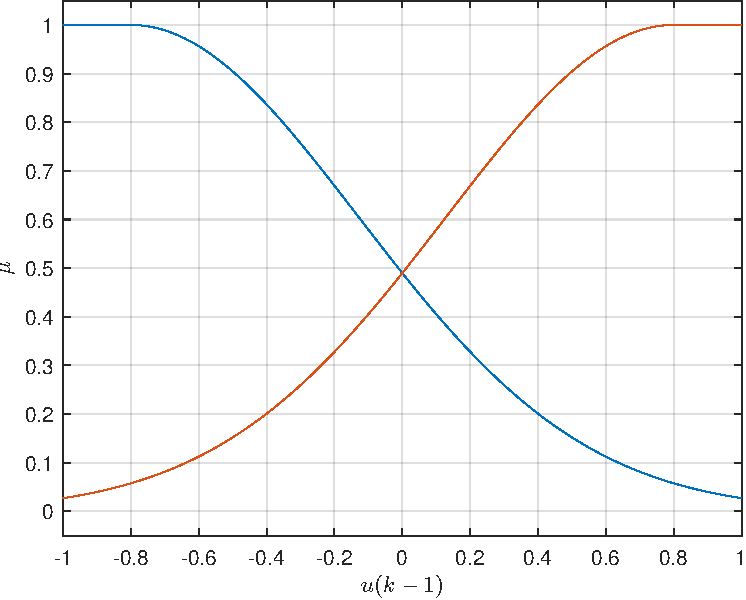
\includegraphics[scale=1]{rysunki/zad5_funkcje_przyn_nr_2_mf_gaussmf}
	\caption{Zastosowane funkcje przynale�no�ci dla $n_\mathrm{r}=2$}
	\label{funkcje_przyn_nr_2_mf_gaussmf_pid}
\end{figure}

\begin{figure}[tb]
	\centering
	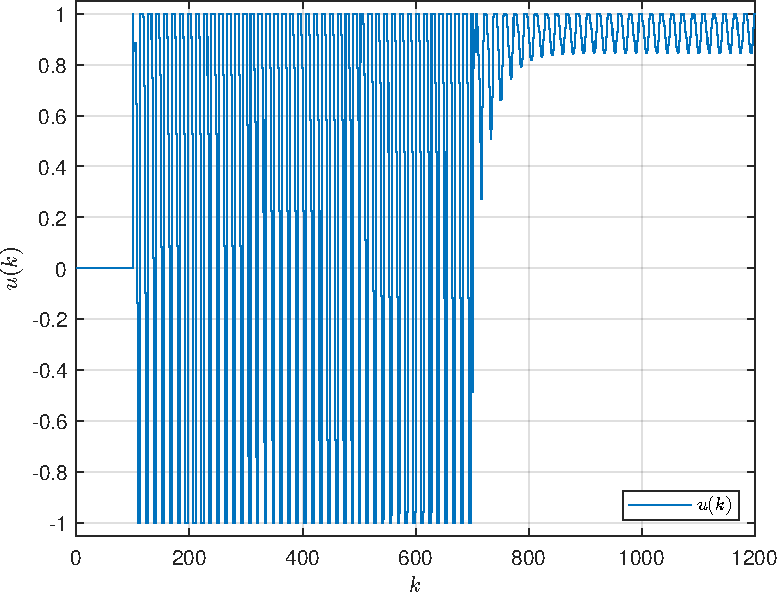
\includegraphics[scale=1]{rysunki/zad5_syg_we_pid_nr_2_mf_gaussmf}
	\caption{Regulator rozmyty PID dla $n_\mathrm{r}=2$ - sygna� steruj�cy}
	\label{syg_we_pid_nr_2_mf_gaussmf}
\end{figure}

\begin{figure}[tb]
	\centering
	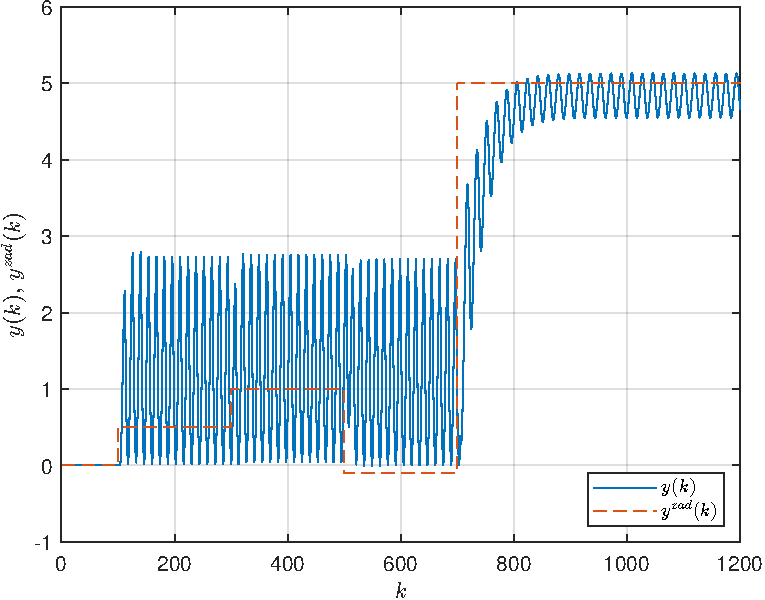
\includegraphics[scale=1]{rysunki/zad5_syg_wy_pid_nr_2_mf_gaussmf}
	\caption{Regulator rozmyty PID dla $n_\mathrm{r}=2$ - sygna� wyj�ciowy i zadany}
	\label{syg_wy_pid_nr_2_mf_gaussmf}
\end{figure}

W kolejnym kroku zwi�kszyli�my liczb� regulator�w lokalnych do $n_\mathrm{r}=3$. Funkcje przynale�no�ci s� widoczne na rys.~\ref{funkcje_przyn_nr_3_mf_gaussmf_pid}. Wyniki symulacji s� przedstawione na rysunkach ~\ref{syg_we_pid_nr_3_mf_gaussmf} oraz \ref{syg_wy_pid_nr_3_mf_gaussmf}. Otrzymana warto�� wska�nika jako�ci regulacji wynosi $E = \num{354.5834}$.


\begin{figure}[tb]
	\centering
	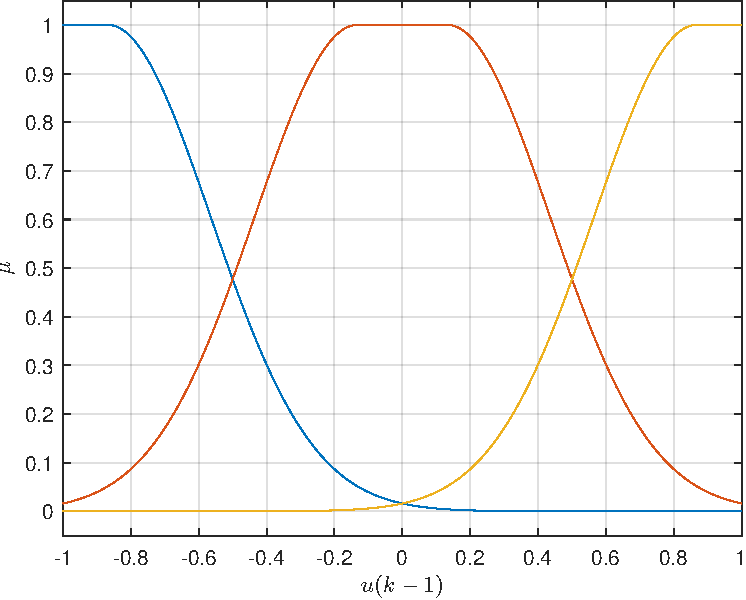
\includegraphics[scale=1]{rysunki/zad5_funkcje_przyn_nr_3_mf_gaussmf}
	\caption{Zastosowane funkcje przynale�no�ci dla $n_\mathrm{r}=3$}
	\label{funkcje_przyn_nr_3_mf_gaussmf_pid}
\end{figure}

\begin{figure}[tb]
	\centering
	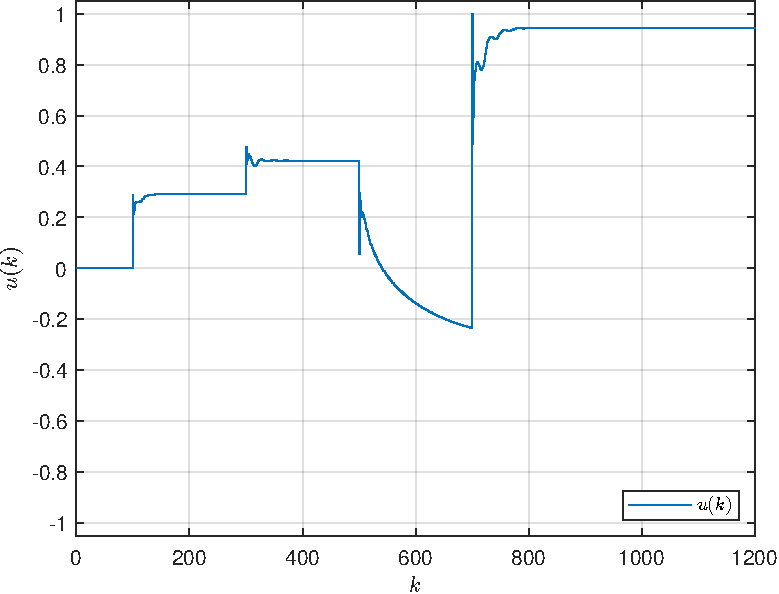
\includegraphics[scale=1]{rysunki/zad5_syg_we_pid_nr_3_mf_gaussmf}
	\caption{Regulator rozmyty PID dla $n_\mathrm{r}=3$ - sygna� steruj�cy}
	\label{syg_we_pid_nr_3_mf_gaussmf}
\end{figure}

\begin{figure}[tb]
	\centering
	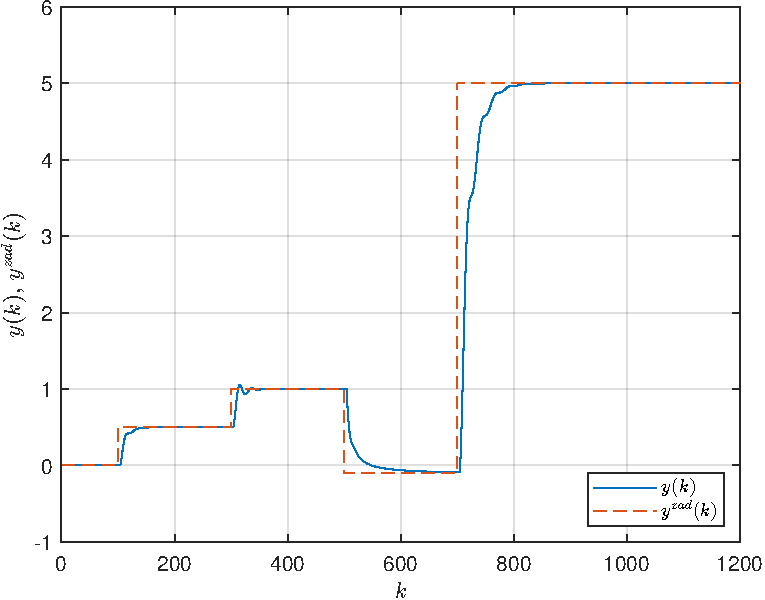
\includegraphics[scale=1]{rysunki/zad5_syg_wy_pid_nr_3_mf_gaussmf}
	\caption{Regulator rozmyty PID dla $n_\mathrm{r}=3$ - sygna� wyj�ciowy i zadany}
	\label{syg_wy_pid_nr_3_mf_gaussmf}
\end{figure}

Nast�pnie sprawdzili�my dzia�anie uk�adu dla $n_\mathrm{r}=4$. Funkcje przynale�no�ci s� widoczne na rys.~\ref{funkcje_przyn_nr_4_mf_gaussmf_pid}. Wyniki symulacji s� przedstawione na rysunkach ~\ref{syg_we_pid_nr_4_mf_gaussmf} oraz \ref{syg_wy_pid_nr_4_mf_gaussmf}. Otrzymana warto�� wska�nika jako�ci regulacji wynosi $E = \num{355.1969}$. Por�wnuj�c warto�ci wska�nika $E$ mo�na zauwa�y�, �e zwi�kszenie liczby regulator�w lokalnych z $n_\mathrm{r}=3$ na $n_\mathrm{r}=4$ nie wp�yn�o w istotny spos�b na jako�� regulacji. W obu przypadkach warto�� zadana jest osi�gana dla r�nych punkt�w pracy. Zwi�kszenie $n_\mathrm{r}$ do warto�ci $4$ pozwoli�o na ca�kowit� eliminacj� przeregulowania, ale nawet dla mniejszej warto�ci $n_\mathrm{r}$ by�o ono bardzo niewielkie.

\begin{figure}[tb]
	\centering
	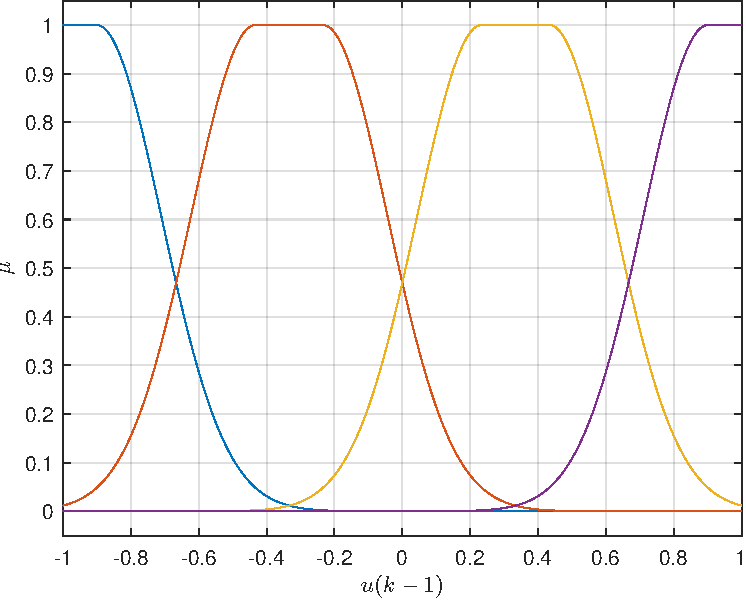
\includegraphics[scale=1]{rysunki/zad5_funkcje_przyn_nr_4_mf_gaussmf}
	\caption{Zastosowane funkcje przynale�no�ci dla $n_\mathrm{r}=4$}
	\label{funkcje_przyn_nr_4_mf_gaussmf_pid}
\end{figure}

\begin{figure}[tb]
	\centering
	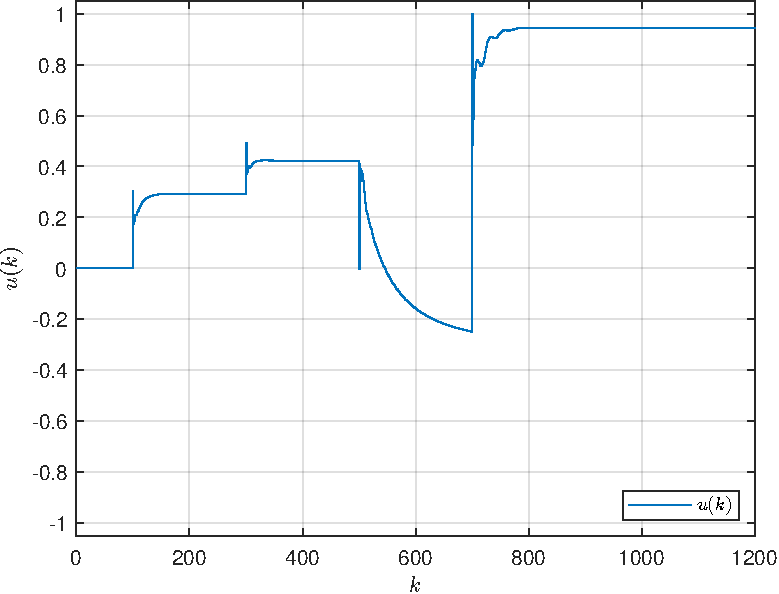
\includegraphics[scale=1]{rysunki/zad5_syg_we_pid_nr_4_mf_gaussmf}
	\caption{Regulator rozmyty PID dla $n_\mathrm{r}=4$ - sygna� steruj�cy}
	\label{syg_we_pid_nr_4_mf_gaussmf}
\end{figure}

\begin{figure}[tb]
	\centering
	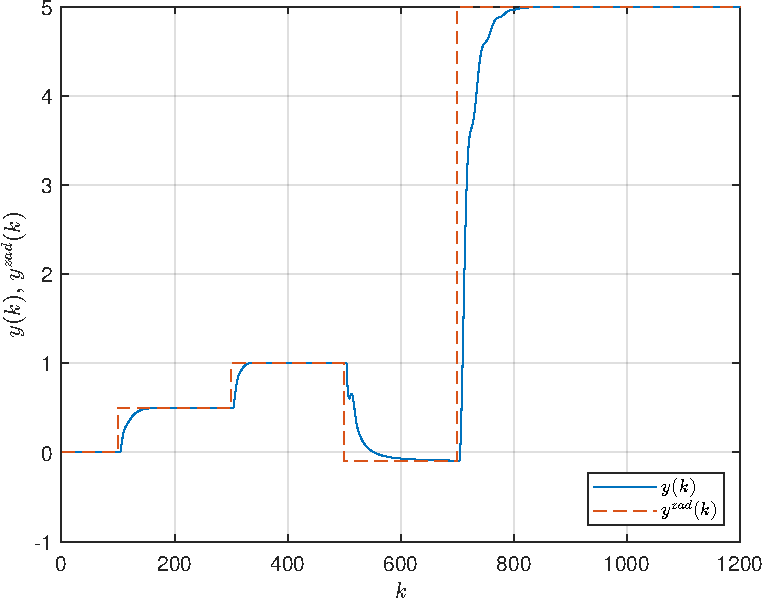
\includegraphics[scale=1]{rysunki/zad5_syg_wy_pid_nr_4_mf_gaussmf}
	\caption{Regulator rozmyty PID dla $n_\mathrm{r}=4$ - sygna� wyj�ciowy i zadany}
	\label{syg_wy_pid_nr_4_mf_gaussmf}
\end{figure}





\section{Funkcje przynale�no�ci tr�jk�tne} 

Na pocz�tku sprawdzili�my dzia�anie uk�adu dla $n_\mathrm{r}=2$. Odpowiadaj�ce tej sytuacji funkcje przynale�no�ci przedstawiono na rys.~\ref{funkcje_przyn_nr_2_mf_trimf_pid}. Wyniki symulacji s� przedstawione na rysunkach ~\ref{syg_we_pid_nr_2_mf_trimf} oraz \ref{syg_wy_pid_nr_2_mf_trimf}. Otrzymana warto�� wska�nika jako�ci regulacji wynosi $E = \num{6.2368e+033}$.

\begin{figure}[tb]
	\centering
	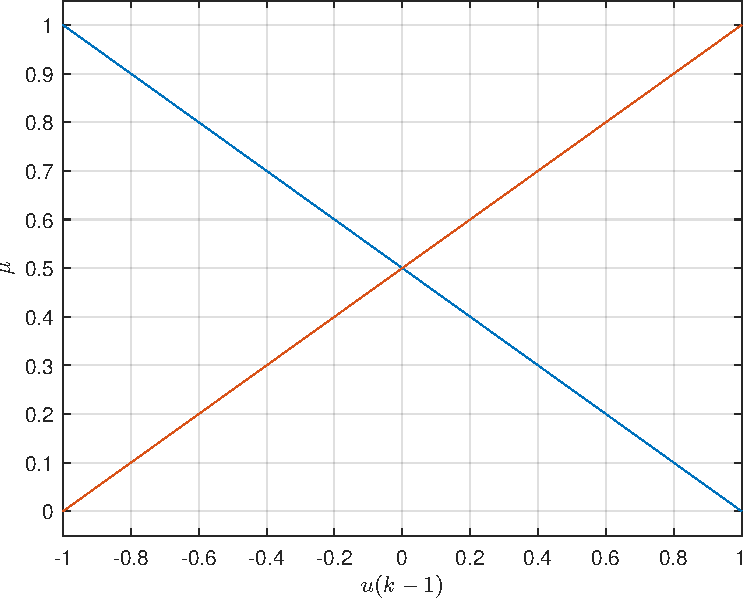
\includegraphics[scale=1]{rysunki/zad5_funkcje_przyn_nr_2_mf_trimf}
	\caption{Zastosowane funkcje przynale�no�ci dla $n_\mathrm{r}=2$}
	\label{funkcje_przyn_nr_2_mf_trimf_pid}
\end{figure}

\begin{figure}[tb]
	\centering
	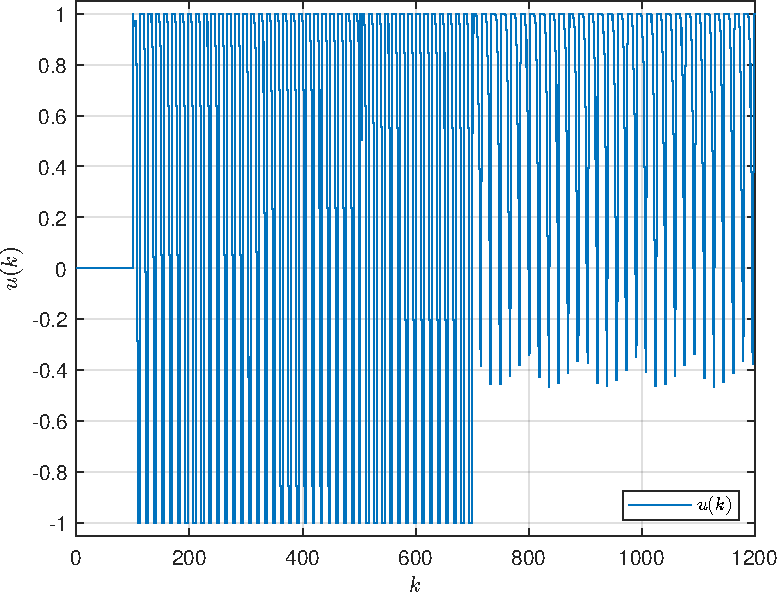
\includegraphics[scale=1]{rysunki/zad5_syg_we_pid_nr_2_mf_trimf}
	\caption{Regulator rozmyty PID dla $n_\mathrm{r}=2$ - sygna� steruj�cy}
	\label{syg_we_pid_nr_2_mf_trimf}
\end{figure}

\begin{figure}[tb]
	\centering
	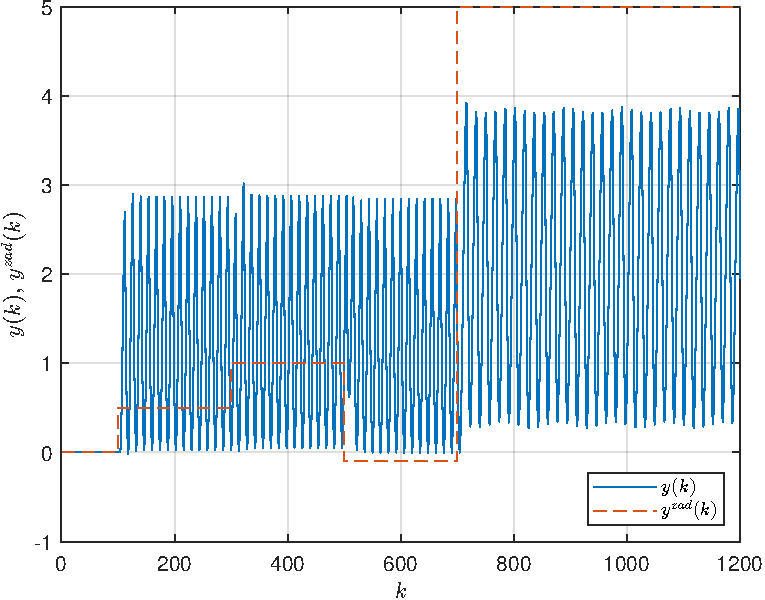
\includegraphics[scale=1]{rysunki/zad5_syg_wy_pid_nr_2_mf_trimf}
	\caption{Regulator rozmyty PID dla $n_\mathrm{r}=2$ - sygna� wyj�ciowy i zadany}
	\label{syg_wy_pid_nr_2_mf_trimf}
\end{figure}

W kolejnym kroku zwi�kszyli�my liczb� regulator�w lokalnych do $n_\mathrm{r}=3$. Funkcje przynale�no�ci s� widoczne na rys.~\ref{funkcje_przyn_nr_3_mf_trimf_pid}. Wyniki symulacji s� przedstawione na rysunkach ~\ref{syg_we_pid_nr_3_mf_trimf} oraz \ref{syg_wy_pid_nr_3_mf_trimf}. Otrzymana warto�� wska�nika jako�ci regulacji wynosi $E = \num{330.9839}$.

\begin{figure}[tb]
	\centering
	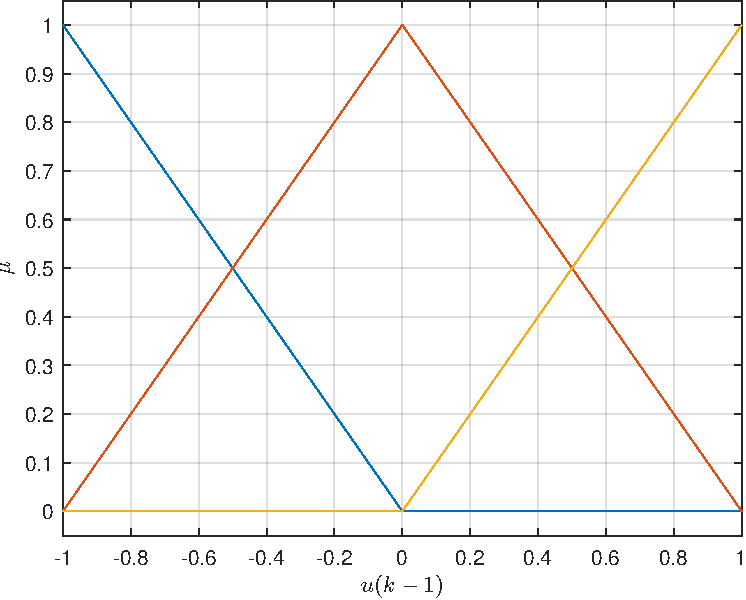
\includegraphics[scale=1]{rysunki/zad5_funkcje_przyn_nr_3_mf_trimf}
	\caption{Zastosowane funkcje przynale�no�ci dla $n_\mathrm{r}=3$}
	\label{funkcje_przyn_nr_3_mf_trimf_pid}
\end{figure}

\begin{figure}[tb]
	\centering
	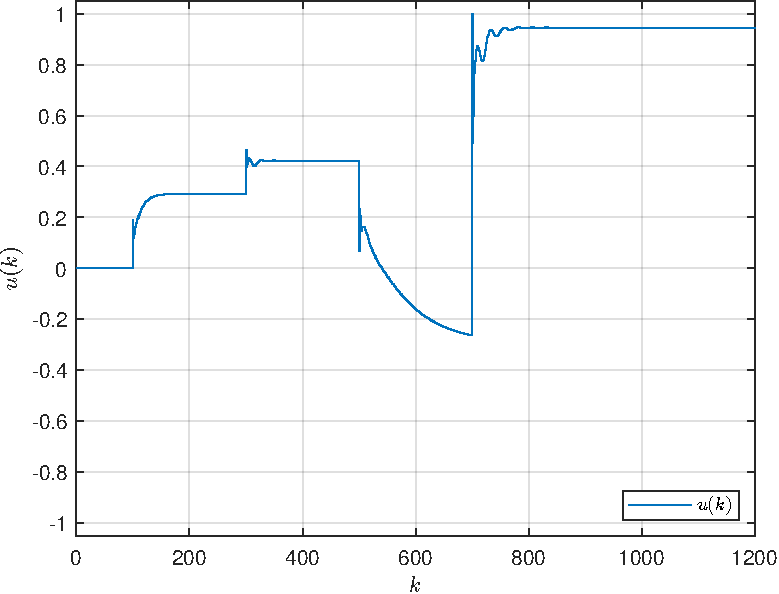
\includegraphics[scale=1]{rysunki/zad5_syg_we_pid_nr_3_mf_trimf}
	\caption{Regulator rozmyty PID dla $n_\mathrm{r}=3$ - sygna� steruj�cy}
	\label{syg_we_pid_nr_3_mf_trimf}
\end{figure}

\begin{figure}[tb]
	\centering
	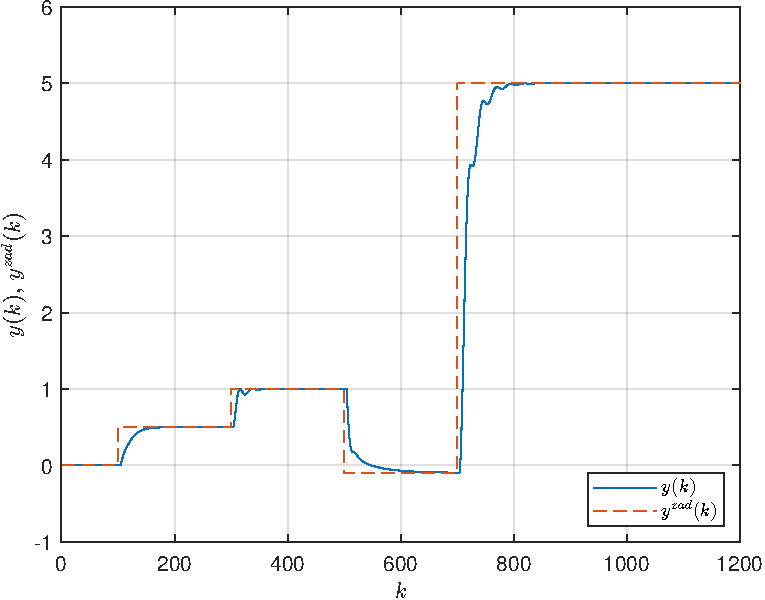
\includegraphics[scale=1]{rysunki/zad5_syg_wy_pid_nr_3_mf_trimf}
	\caption{Regulator rozmyty PID dla $n_\mathrm{r}=3$ - sygna� wyj�ciowy i zadany}
	\label{syg_wy_pid_nr_3_mf_trimf}
\end{figure}

Nast�pnie sprawdzili�my dzia�anie uk�adu dla $n_\mathrm{r}=4$. Funkcje przynale�no�ci s� widoczne na rys.~\ref{funkcje_przyn_nr_4_mf_trimf_pid}. Wyniki symulacji s� przedstawione na rysunkach ~\ref{syg_we_pid_nr_4_mf_trimf} oraz \ref{syg_wy_pid_nr_4_mf_trimf}. Otrzymana warto�� wska�nika jako�ci regulacji wynosi $E = \num{339.2637}$. Por�wnuj�c warto�ci wska�nika $E$ mo�na zauwa�y�, �e zwi�kszenie liczby regulator�w lokalnych z $n_\mathrm{r}=3$ na $n_\mathrm{r}=4$ wp�yn�o na nieznaczne pogorszenie jako�ci regulacji. W obu przypadkach warto�� zadana jest osi�gana dla r�nych punkt�w pracy i nie wyst�puje przeregulowanie. Mo�na tak�e zaobserwowa�, �e wi�ksza warto�� $n_\mathrm{r}$ powoduje szybsze dzia�anie ca�ego systemu.

\begin{figure}[tb]
	\centering
	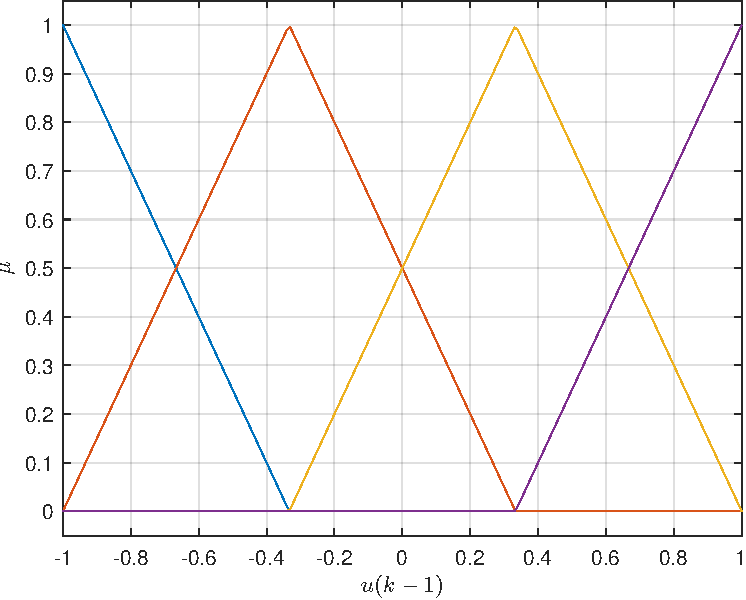
\includegraphics[scale=1]{rysunki/zad5_funkcje_przyn_nr_4_mf_trimf}
	\caption{Zastosowane funkcje przynale�no�ci dla $n_\mathrm{r}=4$}
	\label{funkcje_przyn_nr_4_mf_trimf_pid}
\end{figure}

\begin{figure}[tb]
	\centering
	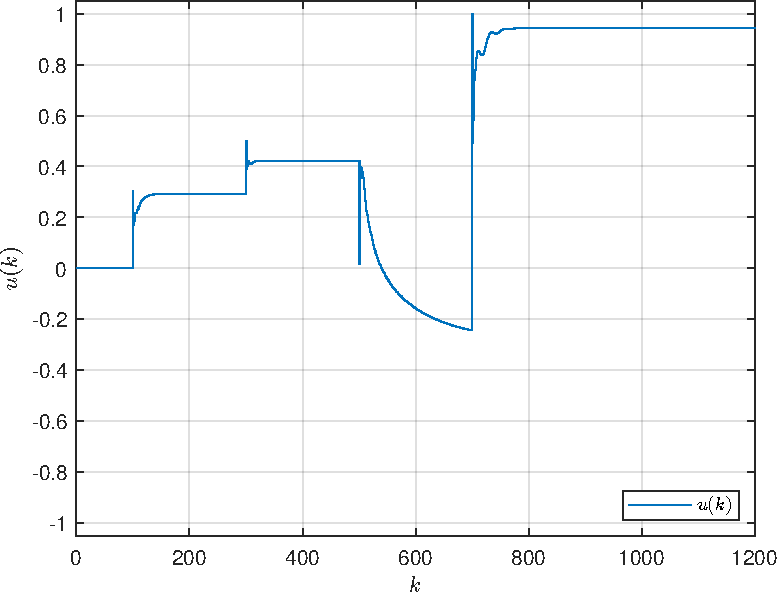
\includegraphics[scale=1]{rysunki/zad5_syg_we_pid_nr_4_mf_trimf}
	\caption{Regulator rozmyty PID dla $n_\mathrm{r}=4$ - sygna� steruj�cy}
	\label{syg_we_pid_nr_4_mf_trimf}
\end{figure}

\begin{figure}[tb]
	\centering
	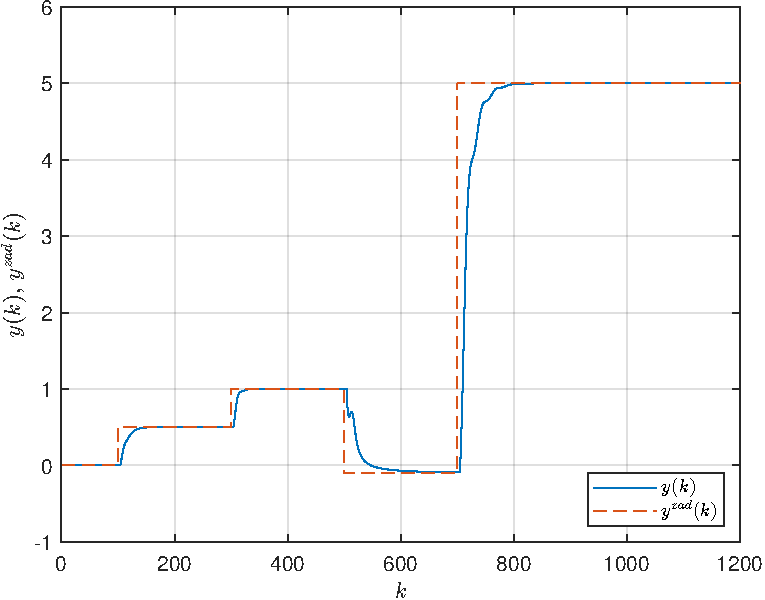
\includegraphics[scale=1]{rysunki/zad5_syg_wy_pid_nr_4_mf_trimf}
	\caption{Regulator rozmyty PID dla $n_\mathrm{r}=4$ - sygna� wyj�ciowy i zadany}
	\label{syg_wy_pid_nr_4_mf_trimf}
\end{figure}



\section{Funkcje przynale�no�ci trapezoidalne}

Na pocz�tku sprawdzili�my dzia�anie uk�adu dla $n_\mathrm{r}=2$. Odpowiadaj�ce tej sytuacji funkcje przynale�no�ci przedstawiono na rys.~\ref{funkcje_przyn_nr_2_mf_trapmf_pid}. Wyniki symulacji s� przedstawione na rysunkach ~\ref{syg_we_pid_nr_2_mf_trapmf} oraz \ref{syg_wy_pid_nr_2_mf_trapmf}. Otrzymana warto�� wska�nika jako�ci regulacji wynosi $E = \num{2.0152e+03}$.

\begin{figure}[tb]
	\centering
	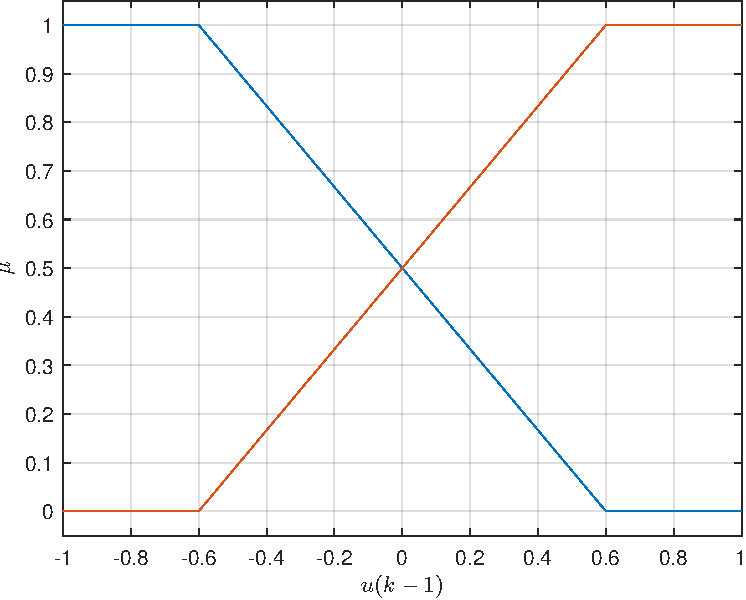
\includegraphics[scale=1]{rysunki/zad5_funkcje_przyn_nr_2_mf_trapmf}
	\caption{Zastosowane funkcje przynale�no�ci dla $n_\mathrm{r}=2$}
	\label{funkcje_przyn_nr_2_mf_trapmf_pid}
\end{figure}

\begin{figure}[tb]
	\centering
	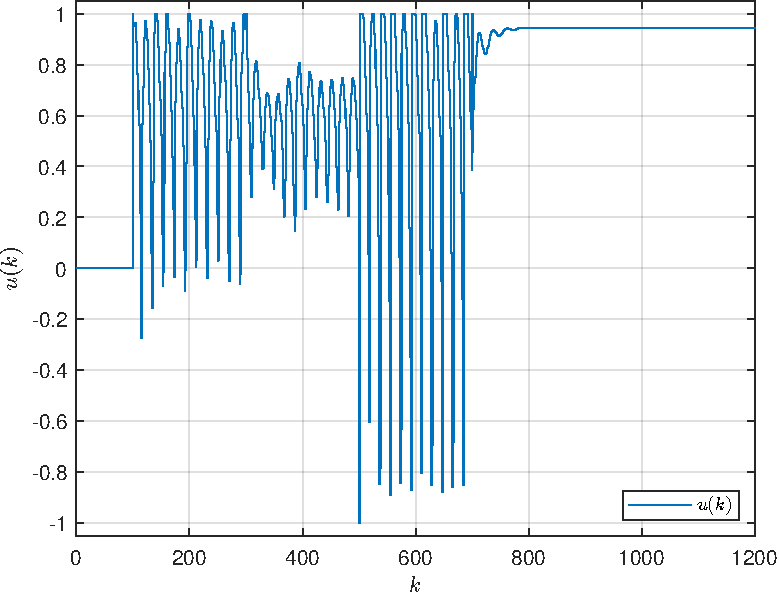
\includegraphics[scale=1]{rysunki/zad5_syg_we_pid_nr_2_mf_trapmf}
	\caption{Regulator rozmyty PID dla $n_\mathrm{r}=2$ - sygna� steruj�cy}
	\label{syg_we_pid_nr_2_mf_trapmf}
\end{figure}

\begin{figure}[tb]
	\centering
	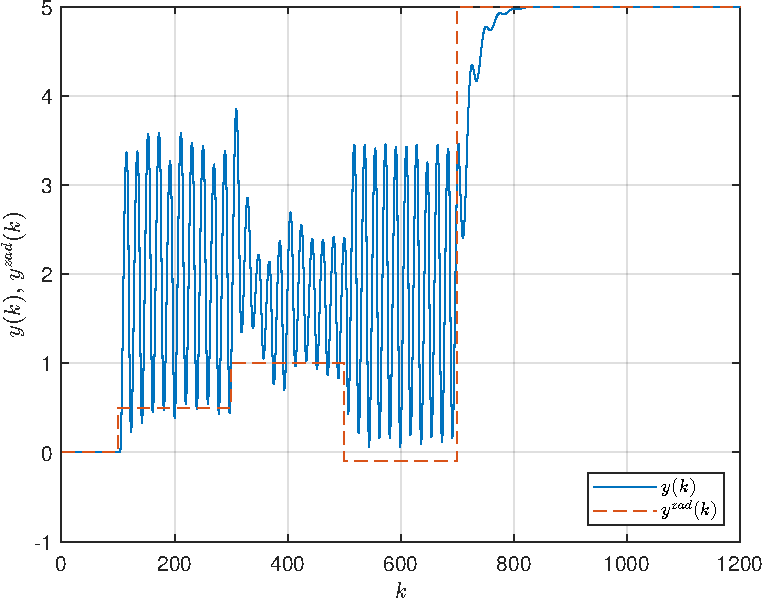
\includegraphics[scale=1]{rysunki/zad5_syg_wy_pid_nr_2_mf_trapmf}
	\caption{Regulator rozmyty PID dla $n_\mathrm{r}=2$ - sygna� wyj�ciowy i zadany}
	\label{syg_wy_pid_nr_2_mf_trapmf}
\end{figure}

W kolejnym kroku zwi�kszyli�my liczb� regulator�w lokalnych do $n_\mathrm{r}=3$. Funkcje przynale�no�ci s� widoczne na rys.~\ref{funkcje_przyn_nr_3_mf_trapmf_pid}. Wyniki symulacji s� przedstawione na rysunkach ~\ref{syg_we_pid_nr_3_mf_trapmf} oraz \ref{syg_wy_pid_nr_3_mf_trapmf}. Otrzymana warto�� wska�nika jako�ci regulacji wynosi $E = \num{385.6358}$.

\begin{figure}[tb]
	\centering
	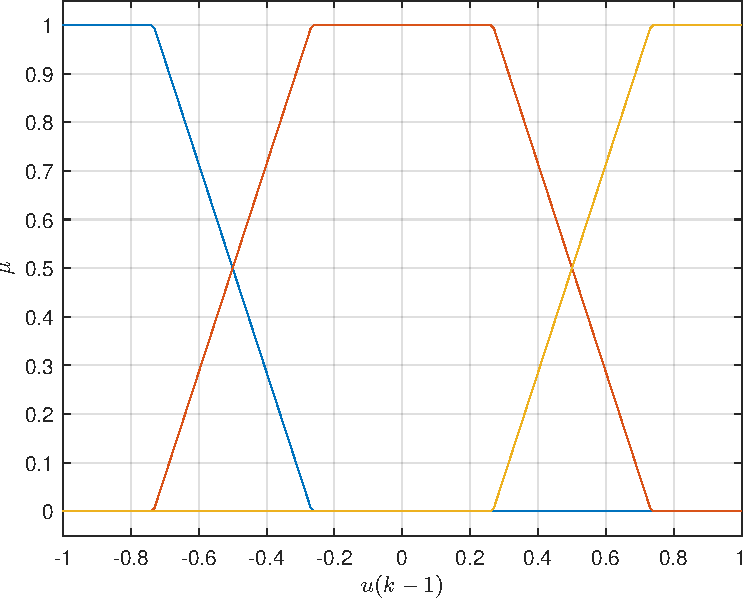
\includegraphics[scale=1]{rysunki/zad5_funkcje_przyn_nr_3_mf_trapmf}
	\caption{Zastosowane funkcje przynale�no�ci dla $n_\mathrm{r}=3$}
	\label{funkcje_przyn_nr_3_mf_trapmf_pid}
\end{figure}

\begin{figure}[tb]
	\centering
	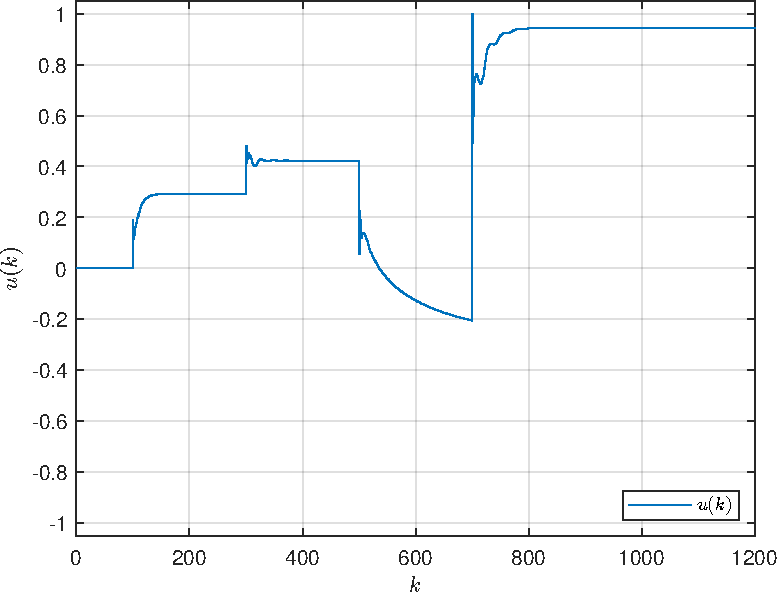
\includegraphics[scale=1]{rysunki/zad5_syg_we_pid_nr_3_mf_trapmf}
	\caption{Regulator rozmyty PID dla $n_\mathrm{r}=3$ - sygna� steruj�cy}
	\label{syg_we_pid_nr_3_mf_trapmf}
\end{figure}

\begin{figure}[tb]
	\centering
	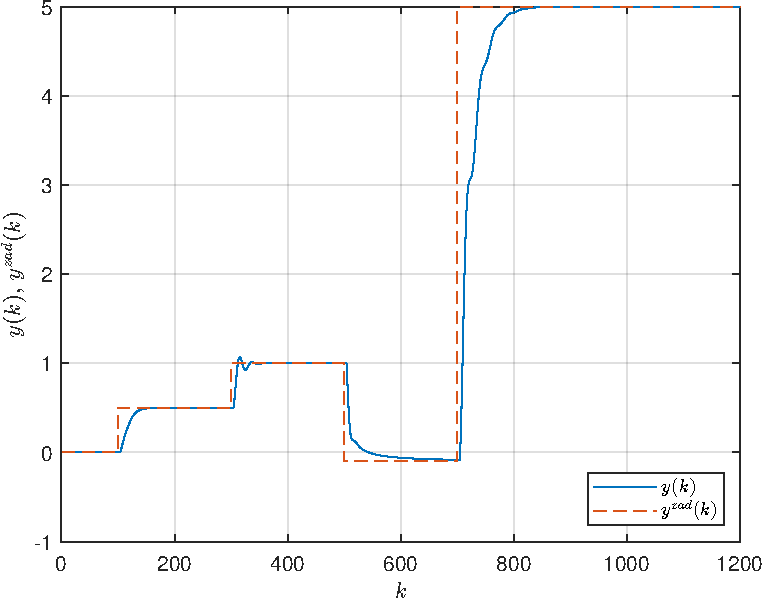
\includegraphics[scale=1]{rysunki/zad5_syg_wy_pid_nr_3_mf_trapmf}
	\caption{Regulator rozmyty PID dla $n_\mathrm{r}=3$ - sygna� wyj�ciowy i zadany}
	\label{syg_wy_pid_nr_3_mf_trapmf}
\end{figure}

Nast�pnie sprawdzili�my dzia�anie uk�adu dla $n_\mathrm{r}=4$. Funkcje przynale�no�ci s� widoczne na rys.~\ref{funkcje_przyn_nr_4_mf_trapmf_pid}. Wyniki symulacji s� przedstawione na rysunkach ~\ref{syg_we_pid_nr_4_mf_trapmf} oraz \ref{syg_wy_pid_nr_4_mf_trapmf}. Otrzymana warto�� wska�nika jako�ci regulacji wynosi $E = \num{368.7729}$. Por�wnuj�c warto�ci wska�nika $E$ mo�na zauwa�y�, �e zwi�kszenie liczby regulator�w lokalnych z $n_\mathrm{r}=3$ na $n_\mathrm{r}=4$ wp�yn�o na popraw� jako�ci regulacji. W obu przypadkach warto�� zadana jest osi�gana dla r�nych punkt�w pracy. Zwi�kszenie $n_\mathrm{r}$ do warto�ci $4$ pozwoli�o na ca�kowit� eliminacj� przeregulowania, ale nawet dla mniejszej warto�ci by�o ono bardzo niewielkie. Mo�na tak�e zaobserwowa�, �e wi�ksza warto�� $n_\mathrm{r}$ powoduje szybsze dzia�anie ca�ego systemu.

\begin{figure}[tb]
	\centering
	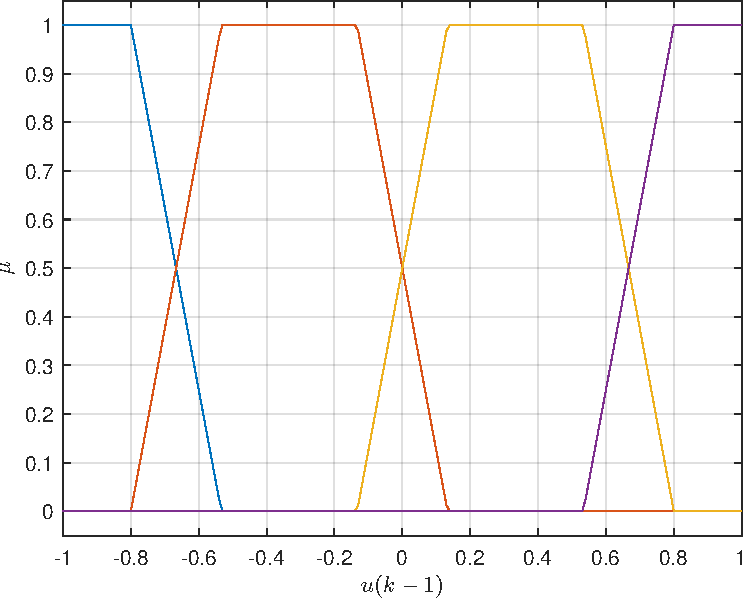
\includegraphics[scale=1]{rysunki/zad5_funkcje_przyn_nr_4_mf_trapmf}
	\caption{Zastosowane funkcje przynale�no�ci dla $n_\mathrm{r}=4$}
	\label{funkcje_przyn_nr_4_mf_trapmf_pid}
\end{figure}

\begin{figure}[tb]
	\centering
	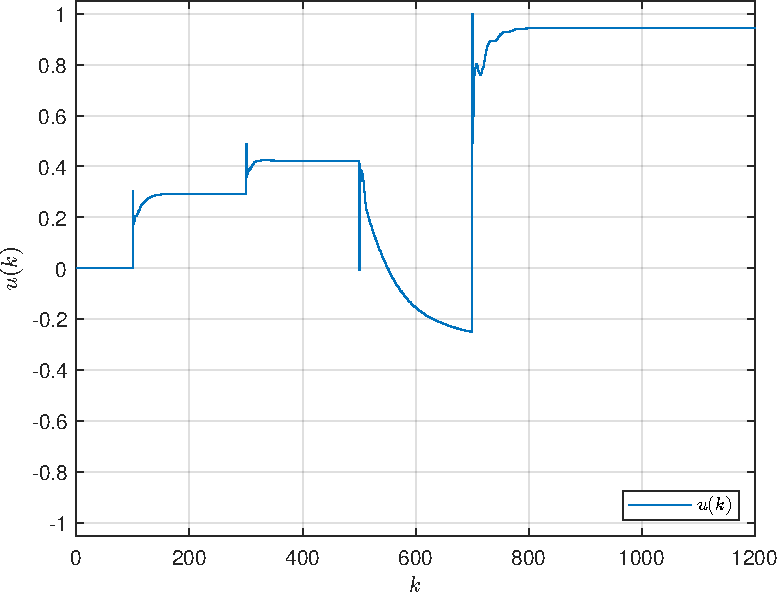
\includegraphics[scale=1]{rysunki/zad5_syg_we_pid_nr_4_mf_trapmf}
	\caption{Regulator rozmyty PID dla $n_\mathrm{r}=4$ - sygna� steruj�cy}
	\label{syg_we_pid_nr_4_mf_trapmf}
\end{figure}

\begin{figure}[tb]
	\centering
	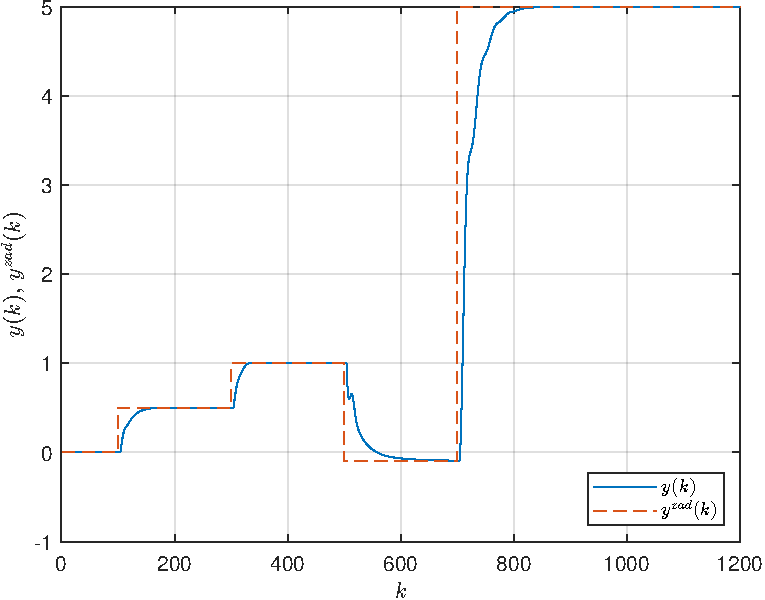
\includegraphics[scale=1]{rysunki/zad5_syg_wy_pid_nr_4_mf_trapmf}
	\caption{Regulator rozmyty PID dla $n_\mathrm{r}=4$ - sygna� wyj�ciowy i zadany}
	\label{syg_wy_pid_nr_4_mf_trapmf}
\end{figure}



\section{Wnioski}
Pod wzgl�dem wska�nika jako�ci najlepsz� regulacj� zapewni�y regulatory, dla kt�rych funkcje przynale�no�ci mia�y kszta�ty tr�jk�tne. Por�wnuj�c regulatory na podstawie samych tylko przebieg�w sygna�u sterujacego oraz wyj�ciowego, ci�ko by�o by jednoznacznie wskaza�, kt�re rozwi�zanie jest najlepsze. Po odpowiednim dostrojeniu regulator�w lokalnych wszystkie uk�ady dzia�a�y satysfakcjonuj�co - warto�ci zadane by�y osi�gane, przeregulowanie, je�li wyst�powa�o, by�o niewielkie i uk�ad dzia�a� szybko. Liczba regulator�w r�wna $n_\mathrm{r}=4$ b�dzie najlepszym kompromisem mi�dzy z�o�ono�ci� algorytmu a uzyskiwan� dok�adno�ci� dzia�ania.

Najwi�kszym problemem przy implementacji rozmytych regulator�w PID jest konieczno�� dostrojenia ka�dego regulatora lokalnego. Wraz ze wzrostem liczby u�ywanych funkcji przynale�no�ci, wzrasta r�wnie� liczba regulator�w PID, kt�re trzeba skalibrowa�. Dlatego cz�sto stosuje si� rozmyte regulatory DMC, kt�rych w zasadzie nie trzeba stroi�, a jedynie wystarczy zebra� lokalne odpowiedzi skokowe.


\end{document}

